 % **************************************************************************************************************
% A Classic Thesis Style
% An Homage to The Elements of Typographic Style
%
% Copyright (C) 2015 André Miede http://www.miede.de
%
% If you like the style then I would appreciate a postcard. My address 
% can be found in the file ClassicThesis.pdf. A collection of the 
% postcards I received so far is available online at 
% http://postcards.miede.de
%
% License:
% This program is free software; you can redistribute it and/or modify
% it under the terms of the GNU General Public License as published by
% the Free Software Foundation; either version 2 of the License, or
% (at your option) any later version.
%
% This program is distributed in the hope that it will be useful,
% but WITHOUT ANY WARRANTY; without even the implied warranty of
% mERCHANTABILITY or FITNESS FOR A PARTICULAR PURPOSE.  See the
% gNU General Public License for more details.
%
% You should have received a copy of the GNU General Public License
% along with this program; see the file COPYING.  If not, write to
% the Free Software Foundation, Inc., 59 Temple Place - Suite 330,
% Boston, MA 02111-1307, USA.
%
% **************************************************************************************************************
\RequirePackage{fix-cm} % fix some latex issues see: http://texdoc.net/texmf-dist/doc/latex/base/fixltx2e.pdf
\documentclass[ twoside,openright,titlepage,numbers=noenddot,headinclude,%1headlines,% letterpaper a4paper
                footinclude=true,cleardoublepage=empty,abstractoff,% <--- obsolete, remove (todo)
                BCOR=5mm,paper=a4,fontsize=11pt,a4paper,%11pt
                frenchb,american%
                ]{scrreprt}

%********************************************************************
% Note: Make all your adjustments in here
%*******************************************************
% ****************************************************************************************************\lstset
% classicthesis-config.tex 
% formerly known as loadpackages.sty, classicthesis-ldpkg.sty, and classicthesis-preamble.sty 
% Use it at the beginning of your ClassicThesis.tex, or as a LaTeX Preamble 
% in your ClassicThesis.{tex,lyx} with % ****************************************************************************************************\lstset
% classicthesis-config.tex 
% formerly known as loadpackages.sty, classicthesis-ldpkg.sty, and classicthesis-preamble.sty 
% Use it at the beginning of your ClassicThesis.tex, or as a LaTeX Preamble 
% in your ClassicThesis.{tex,lyx} with % ****************************************************************************************************\lstset
% classicthesis-config.tex 
% formerly known as loadpackages.sty, classicthesis-ldpkg.sty, and classicthesis-preamble.sty 
% Use it at the beginning of your ClassicThesis.tex, or as a LaTeX Preamble 
% in your ClassicThesis.{tex,lyx} with \input{classicthesis-config}
% ****************************************************************************************************  
% If you like the classicthesis, then I would appreciate a postcard. 
% My address can be found in the file ClassicThesis.pdf. A collection 
% of the postcards I received so far is available online at 
% http://postcards.miede.de
% ****************************************************************************************************


% ****************************************************************************************************
% 0. Set the encoding of your files. UTF-8 is the only sensible encoding nowadays. If you can't read
% äöüßáéçèê∂åëæƒÏ€ then change the encoding setting in your editor, not the line below. If your editor
% does not support utf8 use another editor!
% ****************************************************************************************************
\PassOptionsToPackage{utf8}{inputenc}
	\usepackage{inputenc}
	
%\usepackage{lmodern}
%\usepackage{ae,aecompl}										% Utilisation des fontes vectorielles modernes
% ****************************************************************************************************
% 1. Configure classicthesis for your needs here, e.g., remove "drafting" below 
% in order to deactivate the time-stamp on the pages
% ****************************************************************************************************
\PassOptionsToPackage{eulerchapternumbers,listings,%
					 pdfspacing,%floatperchapter,,%
					 subfig,beramono,eulermath,parts, dottedtoc, linedheaders}{classicthesis}                                        
% ********************************************************************
% Available options for classicthesis.sty 
% (see ClassicThesis.pdf for more information):
% drafting
% parts nochapters linedheaders
% eulerchapternumbers beramono eulermath pdfspacing minionprospacing
% tocaligned dottedtoc manychapters
% listings floatperchapter subfig
% ********************************************************************



% ****************************************************************************************************
% 2. Personal data and user ad-hoc commands
% ****************************************************************************************************
\newcommand{\myTitle}{Résolution de problèmes multi-contacts: méthodes et applications\xspace}
\newcommand{\mySubtitle}{\xspace}
\newcommand{\myDegree}{Doctorat en Informatique\xspace}
\newcommand{\myName}{Mohammed Islam NAAS\xspace}
\newcommand{\myProf}{Jalil Boukhobza\xspace}
\newcommand{\mySupervisor}{Philippe Raipin\xspace}
\newcommand{\myOtherProf}{Laurent Lemarchand\xspace}
\newcommand{\myInstitute}{Orange\xspace}
\newcommand{\myFaculty}{Faculté des Sciences et Techniques\xspace}
\newcommand{\myDepartment}{Lab-STICC UMR 6285\xspace}
\newcommand{\myUni}{Universit\'e de Bretagne Occidentale\xspace}
\newcommand{\myLocation}{Brest, France\xspace}
\newcommand{\myTime}{Décembre 2018}
%\newcommand{\myVersion}{version 0.2\xspace}

% ********************************************************************
% Setup, finetuning, and useful commands
% ********************************************************************
\newcounter{dummy} % necessary for correct hyperlinks (to index, bib, etc.)
\newlength{\abcd} % for ab..z string length calculation
\providecommand{\mLyX}{L\kern-.1667em\lower.25em\hbox{Y}\kern-.125emX\@}
\newcommand{\ie}{i.\,e.}
\newcommand{\Ie}{I.\,e.}
\newcommand{\eg}{e.\,g.}
\newcommand{\Eg}{E.\,g.} 
% ****************************************************************************************************


% ****************************************************************************************************
% 3. Loading some handy packages
% ****************************************************************************************************
% ******************************************************************** 
% Packages with options that might require adjustments
% ******************************************************************** 
%\PassOptionsToPackage{ngerman,american}{babel}   % change this to your language(s)
% Spanish languages need extra options in order to work with this template
\PassOptionsToPackage{spanish,es-lcroman}{babel}
	\usepackage[frenchb,english]{babel}               
	
	\PassOptionsToPackage{numbers,square,sort&compress,sectionbib}{natbib}
		 \usepackage{natbib}	

	\PassOptionsToPackage{fleqn}{amsmath}       % math environments and more by the AMS 
	    \usepackage{amsmath}
	    
	  %  \usepackage{chapterbib}
	\renewcommand{\bibsection}{\section*{Références}}		% Met les références biblio dans un \section (au lieu de \section*)

% ******************************************************************** 
% General useful packages
% ******************************************************************** 
\PassOptionsToPackage{T1}{fontenc} % T2A for cyrillics
    \usepackage{fontenc}     
\usepackage{textcomp} % fix warning with missing font shapes
\usepackage{scrhack} % fix warnings when using KOMA with listings package          
\usepackage{xspace} % to get the spacing after macros right  
\usepackage{mparhack} % get marginpar right
\usepackage{fixltx2e} % fixes some LaTeX stuff --> since 2015 in the LaTeX kernel (see below)
%\usepackage[latest]{latexrelease} % will be used once available in more distributions (ISSUE #107)
\usepackage{eurosym}

\usepackage{multirow}
\usepackage{cellspace}
\usepackage{slashbox}
\usepackage{tabularx}
\usepackage{lscape}

\PassOptionsToPackage{printonlyused,smaller}{acronym} 
    \usepackage{acronym} % nice macros for handling all acronyms in the thesis
    %\renewcommand{\bflabel}[1]{{#1}\hfill} % fix the list of acronyms --> no longer working
   %\renewcommand*{\acsfont}[1]{\textbf{#1}} 
    %\renewcommand*{\aclabelfont}[1]{\acsfont{#1}}
    
% ****************************************************************************************************

\DeclareMathOperator*{\argmin}{\arg\!\min}
\DeclareMathOperator*{\argmax}{\arg\!\max}

% ****************************************************************************************************
% 4. Setup floats: tables, (sub)figures, and captions
% ****************************************************************************************************
\usepackage{tabularx} % better tables
    \setlength{\extrarowheight}{3pt} % increase table row height
\newcommand{\tableheadline}[1]{\multicolumn{1}{c}{\spacedlowsmallcaps{#1}}}
\newcommand{\myfloatalign}{\centering} % to be used with each float for alignment
\usepackage{caption}
% Thanks to cgnieder and Claus Lahiri
% http://tex.stackexchange.com/questions/69349/spacedlowsmallcaps-in-caption-label
% [REMOVED DUE TO OTHER PROBLEMS, SEE ISSUE #82]    
%\DeclareCaptionLabelFormat{smallcaps}{\bothIfFirst{#1}{~}\MakeTextLowercase{\textsc{#2}}}
%\captionsetup{font=small,labelformat=smallcaps} % format=hang,
\captionsetup{font=small} % format=hang,
\usepackage{subfig}  
%%%%%%%% For landscape format an rotation
\usepackage{lscape}
\usepackage{rotating}
% ****************************************************************************************************


% ****************************************************************************************************
% 5. Setup code listings
% ****************************************************************************************************
\usepackage{listings} 
%\lstset{emph={trueIndex,root},emphstyle=\color{BlueViolet}}%\underbar} % for special keywords
\lstset{
	inputencoding=latin1,
	language=[LaTeX]Tex,%C++,
    morekeywords={PassOptionsToPackage,selectlanguage},
    keywordstyle=\color{RoyalBlue},%\bfseries,
    basicstyle=\ttfamily,
    %identifierstyle=\color{NavyBlue},
    commentstyle=\color{Green}\ttfamily,
    stringstyle=\rmfamily,
    numbers=left,%left,%
    numberstyle=\scriptsize,%\tiny
    %stepnumber=5,
    numbersep=8pt,
    showstringspaces=false,
    breaklines=true,
    %frameround=ftff,
    %frame=single,
    columns=fixed,
    belowcaptionskip=.75\baselineskip,
    literate={á}{{\'a}}1 {ã}{{\~a}}1 {é}{{\'e}}1,
    %frame=L
} 
% ****************************************************************************************************             


% ****************************************************************************************************
% 6. PDFLaTeX, hyperreferences and citation backreferences
% ****************************************************************************************************
% ********************************************************************
% Using PDFLaTeX
% ********************************************************************
\PassOptionsToPackage{pdftex,hyperfootnotes=false,pdfpagelabels}{hyperref}
    \usepackage{hyperref}  % backref linktocpage pagebackref
\pdfcompresslevel=9
\pdfadjustspacing=1 
\PassOptionsToPackage{pdftex}{graphicx}
    \usepackage{graphicx} 
 

% ********************************************************************
% Hyperreferences
% ********************************************************************
\hypersetup{%
    %draft, % = no hyperlinking at all (useful in b/w printouts)
    colorlinks=true, linktocpage=true, pdfstartpage=3, pdfstartview=FitV,%
    % uncomment the following line if you want to have black links (e.g., for printing)
    %colorlinks=false, linktocpage=false, pdfstartpage=3, pdfstartview=FitV, pdfborder={0 0 0},%
    breaklinks=true, pdfpagemode=UseNone, pageanchor=true, pdfpagemode=UseOutlines,%
    plainpages=false, bookmarksnumbered, bookmarksopen=true, bookmarksopenlevel=1,%
    hypertexnames=true, pdfhighlight=/O,%nesting=true,%frenchlinks,%
    urlcolor=webbrown, linkcolor=blue, citecolor=webgreen, %pagecolor=RoyalBlue,%
    %urlcolor=Black, linkcolor=Black, citecolor=Black, %pagecolor=Black,%
    pdftitle={\myTitle},%
    pdfauthor={\textcopyright\ \myName, \myUni, \myFaculty},%
    pdfsubject={},%
    pdfkeywords={},%
    pdfcreator={pdfLaTeX},%
    pdfproducer={LaTeX with hyperref and classicthesis}%
}   

% ********************************************************************
% Setup autoreferences
% ********************************************************************
% There are some issues regarding autorefnames
% http://www.ureader.de/msg/136221647.aspx
% http://www.tex.ac.uk/cgi-bin/texfaq2html?label=latexwords
% you have to redefine the makros for the 
% language you use, e.g., american, ngerman
% (as chosen when loading babel/AtBeginDocument)
% ********************************************************************
\makeatletter
\@ifpackageloaded{babel}%
    {%
       \addto\extrasamerican{%
			\renewcommand*{\figureautorefname}{Figure}%
			\renewcommand*{\tableautorefname}{Table}%
			\renewcommand*{\partautorefname}{Part}%
			\renewcommand*{\chapterautorefname}{Chapter}%
			\renewcommand*{\sectionautorefname}{Section}%
			\renewcommand*{\subsectionautorefname}{Section}%
			\renewcommand*{\subsubsectionautorefname}{Section}%     
                }%
       \addto\extrasngerman{% 
			\renewcommand*{\paragraphautorefname}{Absatz}%
			\renewcommand*{\subparagraphautorefname}{Unterabsatz}%
			\renewcommand*{\footnoteautorefname}{Fu\"snote}%
			\renewcommand*{\FancyVerbLineautorefname}{Zeile}%
			\renewcommand*{\theoremautorefname}{Theorem}%
			\renewcommand*{\appendixautorefname}{Anhang}%
			\renewcommand*{\equationautorefname}{Gleichung}%        
			\renewcommand*{\itemautorefname}{Punkt}%
                }%  
            % Fix to getting autorefs for subfigures right (thanks to Belinda Vogt for changing the definition)
            \providecommand{\subfigureautorefname}{\figureautorefname}%             
    }{\relax}
\makeatother


% ****************************************************************************************************
% 7. Last calls before the bar closes
% ****************************************************************************************************
% ********************************************************************
% Development Stuff
% ********************************************************************
\listfiles
%\PassOptionsToPackage{l2tabu,orthodox,abort}{nag}
%   \usepackage{nag}
%\PassOptionsToPackage{warning, all}{onlyamsmath}
%   \usepackage{onlyamsmath}

% ********************************************************************
% Last, but not least...
% ********************************************************************
\usepackage{classicthesis} 
% ****************************************************************************************************


% ****************************************************************************************************
% 8. Further adjustments (experimental)
% ****************************************************************************************************
% ********************************************************************
% Changing the text area
% ********************************************************************
\linespread{1.2} % a bit more for Palatino
%\areaset[current]{312pt}{761pt} % 686 (factor 2.2) + 33 head + 42 head \the\footskip
%\setlength{\marginparwidth}{7em}%
%\setlength{\marginparsep}{2em}%

\areaset[current]{390pt}{761pt} % 686 (factor 2.2) + 33 head + 42 head \the\footskip
%Default: 312pt x 761pt
%Readibility: 390pt x 761pt
%Big: 440pt x 761pt
\setlength{\marginparwidth}{7em}%
\setlength{\marginparsep}{2em}%


% ********************************************************************
% Using different fonts
% ********************************************************************
%\usepackage[oldstylenums]{kpfonts} % oldstyle notextcomp
%\usepackage[osf]{libertine}
%\usepackage[light,condensed,math]{iwona}
%\renewcommand{\sfdefault}{iwona}
%\usepackage{lmodern} % <-- no osf support :-(
%\usepackage{cfr-lm} % 
%\usepackage[urw-garamond]{mathdesign} <-- no osf support :-(
%\usepackage[default,osfigures]{opensans} % scale=0.95 
%\usepackage[sfdefault]{FiraSans}
% ****************************************************************************************************

% ********************************************************************
% Personal Config
% ********************************************************************
\usepackage{epstopdf}
\usepackage{fancyvrb}
\usepackage{caption}
\usepackage{fixltx2e}
\usepackage{url}
\usepackage{amssymb}
\usepackage{listings}
\usepackage{listingsutf8}
%\usepackage{algorithm}
\usepackage{amsthm}
\usepackage{multirow}
\usepackage{array}
\usepackage{minitoc}
\usepackage{breakcites}

%%%% Added by Hamza

\usepackage[final]{pdfpages}
\usepackage[normalem]{ulem}
\mtcselectlanguage{french}
\usepackage{cases}
\usepackage{pifont}
\newcommand{\cmark}{\ding{51}}%
\newcommand{\xmark}{\ding{55}}%
\newcommand{\highlight}[1]{\colorbox{yellow}{$\displaystyle #1$}}
\usepackage{epstopdf}
\usepackage{color, colortbl}
\usepackage[french,onelanguage,vlined, ruled, boxed,linesnumbered]{algorithm2e} % Pour les algorithmes
\definecolor{lightgray}{rgb}{0.83, 0.83, 0.83}
\lstset{%
language=c++,
basicstyle=\small\ttfamily,
backgroundcolor=\color{lightgray},
mathescape=true,
numbers=none}
\SetKwProg{Fn}{Fonction}{}{}
\renewcommand\vdots{%
  \vbox{\baselineskip3pt\lineskiplimit0pt\kern1pt\hbox{.}\hbox{.}\hbox{.}\kern-1pt}}
  %\usepackage{sectsty}
  %\chapterfont{\color{blue}{}\fontfamily{pnc}\selectfont}
%%%%%%%%%%%%%%%%%%%%

\newtheorem{mydef}{Définition}[chapter]

\setcounter{minitocdepth}{1} 
\newcommand\addtotoc[1]{
  \refstepcounter{dummy}
  \addcontentsline{toc}{chapter}{#1}}

\newcolumntype{A}{>{\raggedright\arraybackslash}m{4cm}}
\newcolumntype{L}{>{\raggedright\arraybackslash}m{6cm}}

\newcolumntype{L}[1]{>{\raggedright\let\newline\\\arraybackslash\hspace{0pt}}m{#1}}
\newcolumntype{C}[1]{>{\centering\let\newline\\\arraybackslash\hspace{0pt}}m{#1}}
\newcolumntype{R}[1]{>{\raggedleft\let\newline\\\arraybackslash\hspace{0pt}}m{#1}}

\newtheorem{definition}{Definition}
\newtheorem{theorem}{Theorem}
\newtheorem{lemma}{Lemma}

\lstset{ 
	showspaces=false,              
	showstringspaces=true,        
	showtabs=false,  
	frame=top, 
	frame=bottom,
	numbersep= -5pt,
	numberstyle=\tiny,
	tabsize=2,          
	captionpos=b,          
	breaklines=true,       
	breakatwhitespace=false,    
	escapeinside={\%*}{*)}, 
}

% ****************************************************************************************************  
% If you like the classicthesis, then I would appreciate a postcard. 
% My address can be found in the file ClassicThesis.pdf. A collection 
% of the postcards I received so far is available online at 
% http://postcards.miede.de
% ****************************************************************************************************


% ****************************************************************************************************
% 0. Set the encoding of your files. UTF-8 is the only sensible encoding nowadays. If you can't read
% äöüßáéçèê∂åëæƒÏ€ then change the encoding setting in your editor, not the line below. If your editor
% does not support utf8 use another editor!
% ****************************************************************************************************
\PassOptionsToPackage{utf8}{inputenc}
	\usepackage{inputenc}
	
%\usepackage{lmodern}
%\usepackage{ae,aecompl}										% Utilisation des fontes vectorielles modernes
% ****************************************************************************************************
% 1. Configure classicthesis for your needs here, e.g., remove "drafting" below 
% in order to deactivate the time-stamp on the pages
% ****************************************************************************************************
\PassOptionsToPackage{eulerchapternumbers,listings,%
					 pdfspacing,%floatperchapter,,%
					 subfig,beramono,eulermath,parts, dottedtoc, linedheaders}{classicthesis}                                        
% ********************************************************************
% Available options for classicthesis.sty 
% (see ClassicThesis.pdf for more information):
% drafting
% parts nochapters linedheaders
% eulerchapternumbers beramono eulermath pdfspacing minionprospacing
% tocaligned dottedtoc manychapters
% listings floatperchapter subfig
% ********************************************************************



% ****************************************************************************************************
% 2. Personal data and user ad-hoc commands
% ****************************************************************************************************
\newcommand{\myTitle}{Résolution de problèmes multi-contacts: méthodes et applications\xspace}
\newcommand{\mySubtitle}{\xspace}
\newcommand{\myDegree}{Doctorat en Informatique\xspace}
\newcommand{\myName}{Mohammed Islam NAAS\xspace}
\newcommand{\myProf}{Jalil Boukhobza\xspace}
\newcommand{\mySupervisor}{Philippe Raipin\xspace}
\newcommand{\myOtherProf}{Laurent Lemarchand\xspace}
\newcommand{\myInstitute}{Orange\xspace}
\newcommand{\myFaculty}{Faculté des Sciences et Techniques\xspace}
\newcommand{\myDepartment}{Lab-STICC UMR 6285\xspace}
\newcommand{\myUni}{Universit\'e de Bretagne Occidentale\xspace}
\newcommand{\myLocation}{Brest, France\xspace}
\newcommand{\myTime}{Décembre 2018}
%\newcommand{\myVersion}{version 0.2\xspace}

% ********************************************************************
% Setup, finetuning, and useful commands
% ********************************************************************
\newcounter{dummy} % necessary for correct hyperlinks (to index, bib, etc.)
\newlength{\abcd} % for ab..z string length calculation
\providecommand{\mLyX}{L\kern-.1667em\lower.25em\hbox{Y}\kern-.125emX\@}
\newcommand{\ie}{i.\,e.}
\newcommand{\Ie}{I.\,e.}
\newcommand{\eg}{e.\,g.}
\newcommand{\Eg}{E.\,g.} 
% ****************************************************************************************************


% ****************************************************************************************************
% 3. Loading some handy packages
% ****************************************************************************************************
% ******************************************************************** 
% Packages with options that might require adjustments
% ******************************************************************** 
%\PassOptionsToPackage{ngerman,american}{babel}   % change this to your language(s)
% Spanish languages need extra options in order to work with this template
\PassOptionsToPackage{spanish,es-lcroman}{babel}
	\usepackage[frenchb,english]{babel}               
	
	\PassOptionsToPackage{numbers,square,sort&compress,sectionbib}{natbib}
		 \usepackage{natbib}	

	\PassOptionsToPackage{fleqn}{amsmath}       % math environments and more by the AMS 
	    \usepackage{amsmath}
	    
	  %  \usepackage{chapterbib}
	\renewcommand{\bibsection}{\section*{Références}}		% Met les références biblio dans un \section (au lieu de \section*)

% ******************************************************************** 
% General useful packages
% ******************************************************************** 
\PassOptionsToPackage{T1}{fontenc} % T2A for cyrillics
    \usepackage{fontenc}     
\usepackage{textcomp} % fix warning with missing font shapes
\usepackage{scrhack} % fix warnings when using KOMA with listings package          
\usepackage{xspace} % to get the spacing after macros right  
\usepackage{mparhack} % get marginpar right
\usepackage{fixltx2e} % fixes some LaTeX stuff --> since 2015 in the LaTeX kernel (see below)
%\usepackage[latest]{latexrelease} % will be used once available in more distributions (ISSUE #107)
\usepackage{eurosym}

\usepackage{multirow}
\usepackage{cellspace}
\usepackage{slashbox}
\usepackage{tabularx}
\usepackage{lscape}

\PassOptionsToPackage{printonlyused,smaller}{acronym} 
    \usepackage{acronym} % nice macros for handling all acronyms in the thesis
    %\renewcommand{\bflabel}[1]{{#1}\hfill} % fix the list of acronyms --> no longer working
   %\renewcommand*{\acsfont}[1]{\textbf{#1}} 
    %\renewcommand*{\aclabelfont}[1]{\acsfont{#1}}
    
% ****************************************************************************************************

\DeclareMathOperator*{\argmin}{\arg\!\min}
\DeclareMathOperator*{\argmax}{\arg\!\max}

% ****************************************************************************************************
% 4. Setup floats: tables, (sub)figures, and captions
% ****************************************************************************************************
\usepackage{tabularx} % better tables
    \setlength{\extrarowheight}{3pt} % increase table row height
\newcommand{\tableheadline}[1]{\multicolumn{1}{c}{\spacedlowsmallcaps{#1}}}
\newcommand{\myfloatalign}{\centering} % to be used with each float for alignment
\usepackage{caption}
% Thanks to cgnieder and Claus Lahiri
% http://tex.stackexchange.com/questions/69349/spacedlowsmallcaps-in-caption-label
% [REMOVED DUE TO OTHER PROBLEMS, SEE ISSUE #82]    
%\DeclareCaptionLabelFormat{smallcaps}{\bothIfFirst{#1}{~}\MakeTextLowercase{\textsc{#2}}}
%\captionsetup{font=small,labelformat=smallcaps} % format=hang,
\captionsetup{font=small} % format=hang,
\usepackage{subfig}  
%%%%%%%% For landscape format an rotation
\usepackage{lscape}
\usepackage{rotating}
% ****************************************************************************************************


% ****************************************************************************************************
% 5. Setup code listings
% ****************************************************************************************************
\usepackage{listings} 
%\lstset{emph={trueIndex,root},emphstyle=\color{BlueViolet}}%\underbar} % for special keywords
\lstset{
	inputencoding=latin1,
	language=[LaTeX]Tex,%C++,
    morekeywords={PassOptionsToPackage,selectlanguage},
    keywordstyle=\color{RoyalBlue},%\bfseries,
    basicstyle=\ttfamily,
    %identifierstyle=\color{NavyBlue},
    commentstyle=\color{Green}\ttfamily,
    stringstyle=\rmfamily,
    numbers=left,%left,%
    numberstyle=\scriptsize,%\tiny
    %stepnumber=5,
    numbersep=8pt,
    showstringspaces=false,
    breaklines=true,
    %frameround=ftff,
    %frame=single,
    columns=fixed,
    belowcaptionskip=.75\baselineskip,
    literate={á}{{\'a}}1 {ã}{{\~a}}1 {é}{{\'e}}1,
    %frame=L
} 
% ****************************************************************************************************             


% ****************************************************************************************************
% 6. PDFLaTeX, hyperreferences and citation backreferences
% ****************************************************************************************************
% ********************************************************************
% Using PDFLaTeX
% ********************************************************************
\PassOptionsToPackage{pdftex,hyperfootnotes=false,pdfpagelabels}{hyperref}
    \usepackage{hyperref}  % backref linktocpage pagebackref
\pdfcompresslevel=9
\pdfadjustspacing=1 
\PassOptionsToPackage{pdftex}{graphicx}
    \usepackage{graphicx} 
 

% ********************************************************************
% Hyperreferences
% ********************************************************************
\hypersetup{%
    %draft, % = no hyperlinking at all (useful in b/w printouts)
    colorlinks=true, linktocpage=true, pdfstartpage=3, pdfstartview=FitV,%
    % uncomment the following line if you want to have black links (e.g., for printing)
    %colorlinks=false, linktocpage=false, pdfstartpage=3, pdfstartview=FitV, pdfborder={0 0 0},%
    breaklinks=true, pdfpagemode=UseNone, pageanchor=true, pdfpagemode=UseOutlines,%
    plainpages=false, bookmarksnumbered, bookmarksopen=true, bookmarksopenlevel=1,%
    hypertexnames=true, pdfhighlight=/O,%nesting=true,%frenchlinks,%
    urlcolor=webbrown, linkcolor=blue, citecolor=webgreen, %pagecolor=RoyalBlue,%
    %urlcolor=Black, linkcolor=Black, citecolor=Black, %pagecolor=Black,%
    pdftitle={\myTitle},%
    pdfauthor={\textcopyright\ \myName, \myUni, \myFaculty},%
    pdfsubject={},%
    pdfkeywords={},%
    pdfcreator={pdfLaTeX},%
    pdfproducer={LaTeX with hyperref and classicthesis}%
}   

% ********************************************************************
% Setup autoreferences
% ********************************************************************
% There are some issues regarding autorefnames
% http://www.ureader.de/msg/136221647.aspx
% http://www.tex.ac.uk/cgi-bin/texfaq2html?label=latexwords
% you have to redefine the makros for the 
% language you use, e.g., american, ngerman
% (as chosen when loading babel/AtBeginDocument)
% ********************************************************************
\makeatletter
\@ifpackageloaded{babel}%
    {%
       \addto\extrasamerican{%
			\renewcommand*{\figureautorefname}{Figure}%
			\renewcommand*{\tableautorefname}{Table}%
			\renewcommand*{\partautorefname}{Part}%
			\renewcommand*{\chapterautorefname}{Chapter}%
			\renewcommand*{\sectionautorefname}{Section}%
			\renewcommand*{\subsectionautorefname}{Section}%
			\renewcommand*{\subsubsectionautorefname}{Section}%     
                }%
       \addto\extrasngerman{% 
			\renewcommand*{\paragraphautorefname}{Absatz}%
			\renewcommand*{\subparagraphautorefname}{Unterabsatz}%
			\renewcommand*{\footnoteautorefname}{Fu\"snote}%
			\renewcommand*{\FancyVerbLineautorefname}{Zeile}%
			\renewcommand*{\theoremautorefname}{Theorem}%
			\renewcommand*{\appendixautorefname}{Anhang}%
			\renewcommand*{\equationautorefname}{Gleichung}%        
			\renewcommand*{\itemautorefname}{Punkt}%
                }%  
            % Fix to getting autorefs for subfigures right (thanks to Belinda Vogt for changing the definition)
            \providecommand{\subfigureautorefname}{\figureautorefname}%             
    }{\relax}
\makeatother


% ****************************************************************************************************
% 7. Last calls before the bar closes
% ****************************************************************************************************
% ********************************************************************
% Development Stuff
% ********************************************************************
\listfiles
%\PassOptionsToPackage{l2tabu,orthodox,abort}{nag}
%   \usepackage{nag}
%\PassOptionsToPackage{warning, all}{onlyamsmath}
%   \usepackage{onlyamsmath}

% ********************************************************************
% Last, but not least...
% ********************************************************************
\usepackage{classicthesis} 
% ****************************************************************************************************


% ****************************************************************************************************
% 8. Further adjustments (experimental)
% ****************************************************************************************************
% ********************************************************************
% Changing the text area
% ********************************************************************
\linespread{1.2} % a bit more for Palatino
%\areaset[current]{312pt}{761pt} % 686 (factor 2.2) + 33 head + 42 head \the\footskip
%\setlength{\marginparwidth}{7em}%
%\setlength{\marginparsep}{2em}%

\areaset[current]{390pt}{761pt} % 686 (factor 2.2) + 33 head + 42 head \the\footskip
%Default: 312pt x 761pt
%Readibility: 390pt x 761pt
%Big: 440pt x 761pt
\setlength{\marginparwidth}{7em}%
\setlength{\marginparsep}{2em}%


% ********************************************************************
% Using different fonts
% ********************************************************************
%\usepackage[oldstylenums]{kpfonts} % oldstyle notextcomp
%\usepackage[osf]{libertine}
%\usepackage[light,condensed,math]{iwona}
%\renewcommand{\sfdefault}{iwona}
%\usepackage{lmodern} % <-- no osf support :-(
%\usepackage{cfr-lm} % 
%\usepackage[urw-garamond]{mathdesign} <-- no osf support :-(
%\usepackage[default,osfigures]{opensans} % scale=0.95 
%\usepackage[sfdefault]{FiraSans}
% ****************************************************************************************************

% ********************************************************************
% Personal Config
% ********************************************************************
\usepackage{epstopdf}
\usepackage{fancyvrb}
\usepackage{caption}
\usepackage{fixltx2e}
\usepackage{url}
\usepackage{amssymb}
\usepackage{listings}
\usepackage{listingsutf8}
%\usepackage{algorithm}
\usepackage{amsthm}
\usepackage{multirow}
\usepackage{array}
\usepackage{minitoc}
\usepackage{breakcites}

%%%% Added by Hamza

\usepackage[final]{pdfpages}
\usepackage[normalem]{ulem}
\mtcselectlanguage{french}
\usepackage{cases}
\usepackage{pifont}
\newcommand{\cmark}{\ding{51}}%
\newcommand{\xmark}{\ding{55}}%
\newcommand{\highlight}[1]{\colorbox{yellow}{$\displaystyle #1$}}
\usepackage{epstopdf}
\usepackage{color, colortbl}
\usepackage[french,onelanguage,vlined, ruled, boxed,linesnumbered]{algorithm2e} % Pour les algorithmes
\definecolor{lightgray}{rgb}{0.83, 0.83, 0.83}
\lstset{%
language=c++,
basicstyle=\small\ttfamily,
backgroundcolor=\color{lightgray},
mathescape=true,
numbers=none}
\SetKwProg{Fn}{Fonction}{}{}
\renewcommand\vdots{%
  \vbox{\baselineskip3pt\lineskiplimit0pt\kern1pt\hbox{.}\hbox{.}\hbox{.}\kern-1pt}}
  %\usepackage{sectsty}
  %\chapterfont{\color{blue}{}\fontfamily{pnc}\selectfont}
%%%%%%%%%%%%%%%%%%%%

\newtheorem{mydef}{Définition}[chapter]

\setcounter{minitocdepth}{1} 
\newcommand\addtotoc[1]{
  \refstepcounter{dummy}
  \addcontentsline{toc}{chapter}{#1}}

\newcolumntype{A}{>{\raggedright\arraybackslash}m{4cm}}
\newcolumntype{L}{>{\raggedright\arraybackslash}m{6cm}}

\newcolumntype{L}[1]{>{\raggedright\let\newline\\\arraybackslash\hspace{0pt}}m{#1}}
\newcolumntype{C}[1]{>{\centering\let\newline\\\arraybackslash\hspace{0pt}}m{#1}}
\newcolumntype{R}[1]{>{\raggedleft\let\newline\\\arraybackslash\hspace{0pt}}m{#1}}

\newtheorem{definition}{Definition}
\newtheorem{theorem}{Theorem}
\newtheorem{lemma}{Lemma}

\lstset{ 
	showspaces=false,              
	showstringspaces=true,        
	showtabs=false,  
	frame=top, 
	frame=bottom,
	numbersep= -5pt,
	numberstyle=\tiny,
	tabsize=2,          
	captionpos=b,          
	breaklines=true,       
	breakatwhitespace=false,    
	escapeinside={\%*}{*)}, 
}

% ****************************************************************************************************  
% If you like the classicthesis, then I would appreciate a postcard. 
% My address can be found in the file ClassicThesis.pdf. A collection 
% of the postcards I received so far is available online at 
% http://postcards.miede.de
% ****************************************************************************************************


% ****************************************************************************************************
% 0. Set the encoding of your files. UTF-8 is the only sensible encoding nowadays. If you can't read
% äöüßáéçèê∂åëæƒÏ€ then change the encoding setting in your editor, not the line below. If your editor
% does not support utf8 use another editor!
% ****************************************************************************************************
\PassOptionsToPackage{utf8}{inputenc}
	\usepackage{inputenc}
	
%\usepackage{lmodern}
%\usepackage{ae,aecompl}										% Utilisation des fontes vectorielles modernes
% ****************************************************************************************************
% 1. Configure classicthesis for your needs here, e.g., remove "drafting" below 
% in order to deactivate the time-stamp on the pages
% ****************************************************************************************************
\PassOptionsToPackage{eulerchapternumbers,listings,%
					 pdfspacing,%floatperchapter,,%
					 subfig,beramono,eulermath,parts, dottedtoc, linedheaders}{classicthesis}                                        
% ********************************************************************
% Available options for classicthesis.sty 
% (see ClassicThesis.pdf for more information):
% drafting
% parts nochapters linedheaders
% eulerchapternumbers beramono eulermath pdfspacing minionprospacing
% tocaligned dottedtoc manychapters
% listings floatperchapter subfig
% ********************************************************************



% ****************************************************************************************************
% 2. Personal data and user ad-hoc commands
% ****************************************************************************************************
\newcommand{\myTitle}{Résolution de problèmes multi-contacts: méthodes et applications\xspace}
\newcommand{\mySubtitle}{\xspace}
\newcommand{\myDegree}{Doctorat en Informatique\xspace}
\newcommand{\myName}{Mohammed Islam NAAS\xspace}
\newcommand{\myProf}{Jalil Boukhobza\xspace}
\newcommand{\mySupervisor}{Philippe Raipin\xspace}
\newcommand{\myOtherProf}{Laurent Lemarchand\xspace}
\newcommand{\myInstitute}{Orange\xspace}
\newcommand{\myFaculty}{Faculté des Sciences et Techniques\xspace}
\newcommand{\myDepartment}{Lab-STICC UMR 6285\xspace}
\newcommand{\myUni}{Universit\'e de Bretagne Occidentale\xspace}
\newcommand{\myLocation}{Brest, France\xspace}
\newcommand{\myTime}{Décembre 2018}
%\newcommand{\myVersion}{version 0.2\xspace}

% ********************************************************************
% Setup, finetuning, and useful commands
% ********************************************************************
\newcounter{dummy} % necessary for correct hyperlinks (to index, bib, etc.)
\newlength{\abcd} % for ab..z string length calculation
\providecommand{\mLyX}{L\kern-.1667em\lower.25em\hbox{Y}\kern-.125emX\@}
\newcommand{\ie}{i.\,e.}
\newcommand{\Ie}{I.\,e.}
\newcommand{\eg}{e.\,g.}
\newcommand{\Eg}{E.\,g.} 
% ****************************************************************************************************


% ****************************************************************************************************
% 3. Loading some handy packages
% ****************************************************************************************************
% ******************************************************************** 
% Packages with options that might require adjustments
% ******************************************************************** 
%\PassOptionsToPackage{ngerman,american}{babel}   % change this to your language(s)
% Spanish languages need extra options in order to work with this template
\PassOptionsToPackage{spanish,es-lcroman}{babel}
	\usepackage[frenchb,english]{babel}               
	
	\PassOptionsToPackage{numbers,square,sort&compress,sectionbib}{natbib}
		 \usepackage{natbib}	

	\PassOptionsToPackage{fleqn}{amsmath}       % math environments and more by the AMS 
	    \usepackage{amsmath}
	    
	  %  \usepackage{chapterbib}
	\renewcommand{\bibsection}{\section*{Références}}		% Met les références biblio dans un \section (au lieu de \section*)

% ******************************************************************** 
% General useful packages
% ******************************************************************** 
\PassOptionsToPackage{T1}{fontenc} % T2A for cyrillics
    \usepackage{fontenc}     
\usepackage{textcomp} % fix warning with missing font shapes
\usepackage{scrhack} % fix warnings when using KOMA with listings package          
\usepackage{xspace} % to get the spacing after macros right  
\usepackage{mparhack} % get marginpar right
\usepackage{fixltx2e} % fixes some LaTeX stuff --> since 2015 in the LaTeX kernel (see below)
%\usepackage[latest]{latexrelease} % will be used once available in more distributions (ISSUE #107)
\usepackage{eurosym}

\usepackage{multirow}
\usepackage{cellspace}
\usepackage{slashbox}
\usepackage{tabularx}
\usepackage{lscape}

\PassOptionsToPackage{printonlyused,smaller}{acronym} 
    \usepackage{acronym} % nice macros for handling all acronyms in the thesis
    %\renewcommand{\bflabel}[1]{{#1}\hfill} % fix the list of acronyms --> no longer working
   %\renewcommand*{\acsfont}[1]{\textbf{#1}} 
    %\renewcommand*{\aclabelfont}[1]{\acsfont{#1}}
    
% ****************************************************************************************************

\DeclareMathOperator*{\argmin}{\arg\!\min}
\DeclareMathOperator*{\argmax}{\arg\!\max}

% ****************************************************************************************************
% 4. Setup floats: tables, (sub)figures, and captions
% ****************************************************************************************************
\usepackage{tabularx} % better tables
    \setlength{\extrarowheight}{3pt} % increase table row height
\newcommand{\tableheadline}[1]{\multicolumn{1}{c}{\spacedlowsmallcaps{#1}}}
\newcommand{\myfloatalign}{\centering} % to be used with each float for alignment
\usepackage{caption}
% Thanks to cgnieder and Claus Lahiri
% http://tex.stackexchange.com/questions/69349/spacedlowsmallcaps-in-caption-label
% [REMOVED DUE TO OTHER PROBLEMS, SEE ISSUE #82]    
%\DeclareCaptionLabelFormat{smallcaps}{\bothIfFirst{#1}{~}\MakeTextLowercase{\textsc{#2}}}
%\captionsetup{font=small,labelformat=smallcaps} % format=hang,
\captionsetup{font=small} % format=hang,
\usepackage{subfig}  
%%%%%%%% For landscape format an rotation
\usepackage{lscape}
\usepackage{rotating}
% ****************************************************************************************************


% ****************************************************************************************************
% 5. Setup code listings
% ****************************************************************************************************
\usepackage{listings} 
%\lstset{emph={trueIndex,root},emphstyle=\color{BlueViolet}}%\underbar} % for special keywords
\lstset{
	inputencoding=latin1,
	language=[LaTeX]Tex,%C++,
    morekeywords={PassOptionsToPackage,selectlanguage},
    keywordstyle=\color{RoyalBlue},%\bfseries,
    basicstyle=\ttfamily,
    %identifierstyle=\color{NavyBlue},
    commentstyle=\color{Green}\ttfamily,
    stringstyle=\rmfamily,
    numbers=left,%left,%
    numberstyle=\scriptsize,%\tiny
    %stepnumber=5,
    numbersep=8pt,
    showstringspaces=false,
    breaklines=true,
    %frameround=ftff,
    %frame=single,
    columns=fixed,
    belowcaptionskip=.75\baselineskip,
    literate={á}{{\'a}}1 {ã}{{\~a}}1 {é}{{\'e}}1,
    %frame=L
} 
% ****************************************************************************************************             


% ****************************************************************************************************
% 6. PDFLaTeX, hyperreferences and citation backreferences
% ****************************************************************************************************
% ********************************************************************
% Using PDFLaTeX
% ********************************************************************
\PassOptionsToPackage{pdftex,hyperfootnotes=false,pdfpagelabels}{hyperref}
    \usepackage{hyperref}  % backref linktocpage pagebackref
\pdfcompresslevel=9
\pdfadjustspacing=1 
\PassOptionsToPackage{pdftex}{graphicx}
    \usepackage{graphicx} 
 

% ********************************************************************
% Hyperreferences
% ********************************************************************
\hypersetup{%
    %draft, % = no hyperlinking at all (useful in b/w printouts)
    colorlinks=true, linktocpage=true, pdfstartpage=3, pdfstartview=FitV,%
    % uncomment the following line if you want to have black links (e.g., for printing)
    %colorlinks=false, linktocpage=false, pdfstartpage=3, pdfstartview=FitV, pdfborder={0 0 0},%
    breaklinks=true, pdfpagemode=UseNone, pageanchor=true, pdfpagemode=UseOutlines,%
    plainpages=false, bookmarksnumbered, bookmarksopen=true, bookmarksopenlevel=1,%
    hypertexnames=true, pdfhighlight=/O,%nesting=true,%frenchlinks,%
    urlcolor=webbrown, linkcolor=blue, citecolor=webgreen, %pagecolor=RoyalBlue,%
    %urlcolor=Black, linkcolor=Black, citecolor=Black, %pagecolor=Black,%
    pdftitle={\myTitle},%
    pdfauthor={\textcopyright\ \myName, \myUni, \myFaculty},%
    pdfsubject={},%
    pdfkeywords={},%
    pdfcreator={pdfLaTeX},%
    pdfproducer={LaTeX with hyperref and classicthesis}%
}   

% ********************************************************************
% Setup autoreferences
% ********************************************************************
% There are some issues regarding autorefnames
% http://www.ureader.de/msg/136221647.aspx
% http://www.tex.ac.uk/cgi-bin/texfaq2html?label=latexwords
% you have to redefine the makros for the 
% language you use, e.g., american, ngerman
% (as chosen when loading babel/AtBeginDocument)
% ********************************************************************
\makeatletter
\@ifpackageloaded{babel}%
    {%
       \addto\extrasamerican{%
			\renewcommand*{\figureautorefname}{Figure}%
			\renewcommand*{\tableautorefname}{Table}%
			\renewcommand*{\partautorefname}{Part}%
			\renewcommand*{\chapterautorefname}{Chapter}%
			\renewcommand*{\sectionautorefname}{Section}%
			\renewcommand*{\subsectionautorefname}{Section}%
			\renewcommand*{\subsubsectionautorefname}{Section}%     
                }%
       \addto\extrasngerman{% 
			\renewcommand*{\paragraphautorefname}{Absatz}%
			\renewcommand*{\subparagraphautorefname}{Unterabsatz}%
			\renewcommand*{\footnoteautorefname}{Fu\"snote}%
			\renewcommand*{\FancyVerbLineautorefname}{Zeile}%
			\renewcommand*{\theoremautorefname}{Theorem}%
			\renewcommand*{\appendixautorefname}{Anhang}%
			\renewcommand*{\equationautorefname}{Gleichung}%        
			\renewcommand*{\itemautorefname}{Punkt}%
                }%  
            % Fix to getting autorefs for subfigures right (thanks to Belinda Vogt for changing the definition)
            \providecommand{\subfigureautorefname}{\figureautorefname}%             
    }{\relax}
\makeatother


% ****************************************************************************************************
% 7. Last calls before the bar closes
% ****************************************************************************************************
% ********************************************************************
% Development Stuff
% ********************************************************************
\listfiles
%\PassOptionsToPackage{l2tabu,orthodox,abort}{nag}
%   \usepackage{nag}
%\PassOptionsToPackage{warning, all}{onlyamsmath}
%   \usepackage{onlyamsmath}

% ********************************************************************
% Last, but not least...
% ********************************************************************
\usepackage{classicthesis} 
% ****************************************************************************************************


% ****************************************************************************************************
% 8. Further adjustments (experimental)
% ****************************************************************************************************
% ********************************************************************
% Changing the text area
% ********************************************************************
\linespread{1.2} % a bit more for Palatino
%\areaset[current]{312pt}{761pt} % 686 (factor 2.2) + 33 head + 42 head \the\footskip
%\setlength{\marginparwidth}{7em}%
%\setlength{\marginparsep}{2em}%

\areaset[current]{390pt}{761pt} % 686 (factor 2.2) + 33 head + 42 head \the\footskip
%Default: 312pt x 761pt
%Readibility: 390pt x 761pt
%Big: 440pt x 761pt
\setlength{\marginparwidth}{7em}%
\setlength{\marginparsep}{2em}%


% ********************************************************************
% Using different fonts
% ********************************************************************
%\usepackage[oldstylenums]{kpfonts} % oldstyle notextcomp
%\usepackage[osf]{libertine}
%\usepackage[light,condensed,math]{iwona}
%\renewcommand{\sfdefault}{iwona}
%\usepackage{lmodern} % <-- no osf support :-(
%\usepackage{cfr-lm} % 
%\usepackage[urw-garamond]{mathdesign} <-- no osf support :-(
%\usepackage[default,osfigures]{opensans} % scale=0.95 
%\usepackage[sfdefault]{FiraSans}
% ****************************************************************************************************

% ********************************************************************
% Personal Config
% ********************************************************************
\usepackage{epstopdf}
\usepackage{fancyvrb}
\usepackage{caption}
\usepackage{fixltx2e}
\usepackage{url}
\usepackage{amssymb}
\usepackage{listings}
\usepackage{listingsutf8}
%\usepackage{algorithm}
\usepackage{amsthm}
\usepackage{multirow}
\usepackage{array}
\usepackage{minitoc}
\usepackage{breakcites}

%%%% Added by Hamza

\usepackage[final]{pdfpages}
\usepackage[normalem]{ulem}
\mtcselectlanguage{french}
\usepackage{cases}
\usepackage{pifont}
\newcommand{\cmark}{\ding{51}}%
\newcommand{\xmark}{\ding{55}}%
\newcommand{\highlight}[1]{\colorbox{yellow}{$\displaystyle #1$}}
\usepackage{epstopdf}
\usepackage{color, colortbl}
\usepackage[french,onelanguage,vlined, ruled, boxed,linesnumbered]{algorithm2e} % Pour les algorithmes
\definecolor{lightgray}{rgb}{0.83, 0.83, 0.83}
\lstset{%
language=c++,
basicstyle=\small\ttfamily,
backgroundcolor=\color{lightgray},
mathescape=true,
numbers=none}
\SetKwProg{Fn}{Fonction}{}{}
\renewcommand\vdots{%
  \vbox{\baselineskip3pt\lineskiplimit0pt\kern1pt\hbox{.}\hbox{.}\hbox{.}\kern-1pt}}
  %\usepackage{sectsty}
  %\chapterfont{\color{blue}{}\fontfamily{pnc}\selectfont}
%%%%%%%%%%%%%%%%%%%%

\newtheorem{mydef}{Définition}[chapter]

\setcounter{minitocdepth}{1} 
\newcommand\addtotoc[1]{
  \refstepcounter{dummy}
  \addcontentsline{toc}{chapter}{#1}}

\newcolumntype{A}{>{\raggedright\arraybackslash}m{4cm}}
\newcolumntype{L}{>{\raggedright\arraybackslash}m{6cm}}

\newcolumntype{L}[1]{>{\raggedright\let\newline\\\arraybackslash\hspace{0pt}}m{#1}}
\newcolumntype{C}[1]{>{\centering\let\newline\\\arraybackslash\hspace{0pt}}m{#1}}
\newcolumntype{R}[1]{>{\raggedleft\let\newline\\\arraybackslash\hspace{0pt}}m{#1}}

\newtheorem{definition}{Definition}
\newtheorem{theorem}{Theorem}
\newtheorem{lemma}{Lemma}

\lstset{ 
	showspaces=false,              
	showstringspaces=true,        
	showtabs=false,  
	frame=top, 
	frame=bottom,
	numbersep= -5pt,
	numberstyle=\tiny,
	tabsize=2,          
	captionpos=b,          
	breaklines=true,       
	breakatwhitespace=false,    
	escapeinside={\%*}{*)}, 
}



%********************************************************************
% Bibliographies
%*******************************************************


%********************************************************************
% Hyphenation
%*******************************************************
%\hyphenation{put special hyphenation here}

% ********************************************************************
% 
%*******************************************************
\begin{document}
\frenchspacing
\raggedbottom
\selectlanguage{french} % american ngerman
%\renewcommand*{\bibname}{new name}
%\setbibpreamble{}
\pagenumbering{roman}
\pagestyle{plain}
%********************************************************************
% Frontmatter
%*******************************************************
\begingroup 
    \let\clearpage\relax
    \let\cleardoublepage\relax
    \let\cleardoublepage\relax
\includepdf[pages={1}]{FrontBackmatter/Titlepage_bis.pdf}

\clearpage\null\newpage
\cleardoublepage
%*******************************************************
% Dedication
%*******************************************************
%\thispagestyle{empty}
%\phantomsection 
\refstepcounter{dummy}
%\cleardoublepage
\pdfbookmark[1]{Remerciements}{Remerciements}
\chapter*{Remerciements}

Ce manuscrit de thèse est le fruit de trois années de dur labeur passées au Laboratoire de Mathématiques et Physiques (LAMPS) de l'Université de Perpignan Via Domitia au sein de l'équipe Mathématique.\\

Je remercie donc tout naturellement et très chaleureusement l’équipe qui m’a encadré, sans laquelle cette thèse n’aurait jamais vu le jour. En premier lieu mon directeur de thèse, \textbf{Mikaël Barboteu}, pour m'avoir proposé le sujet de thèse, pour sa confiance en moi, pour son travail de suivi, pour ses remarques enrichissantes, tout en soulignant sa gentillesse et sa bienveillance. Je tiens également à remercier \textbf{Stéphane Abide} pour qui je voudrais exprimer mon entière considération, pour le temps qu'il m'a dédié tout au long de ma thèse, pour son travail de suivi et ses précieux conseils. Je tiens enfin à remercier \textbf{Serge Dumont} pour son travail de suivi, pour ses contributions, et sa disponibilité malgré la distance.\\

Je tiens également à remercier les Professeurs Frédéric Lebon et Yves Renard d'avoir accepté la charge de rapporteurs de cette thèse, ainsi que l'ensemble des autres membres du jury pour avoir fait le déplacement à Perpignan à l'occasion de ma soutenance.\\
Le bon déroulement de ma thèse je le dois aussi à l’ensemble des membres de l’équipe du laboratoire LAMPS, avec une mention spéciale à \textbf{Joëlle Sullian}, \textbf{Sylvia Munoz} et \textbf{Michel Cayrol} pour leur soutien infaillible, leurs encouragements et leurs accompagnements précieux durant cette thèse, notamment dans les démarches administratives auprès de l'université et de l'école doctorale.\\

Cette thèse était aussi l’occasion de rencontrer des collègues formidables sans qui le travail au bureau aurait été ennuyant. Un grand merci à \textbf{Farah Benmouhoub} et \textbf{Dorra Benkhalifa} pour leurs anecdotes aussi drôles les unes que les autres, à \textbf{Mohammed Islam Naas} pour ses conseils bienveillants, et une mention spéciale à mon ami \textbf{Rami louati} pour tous les bons moments de détente passés ensemble, sans oublier tous les autres collègues du laboratoire qui ont contribué de près ou de loin à la réussite de ce travail.\\

Sans oublier les plus grands remerciements du monde à mes parents, à ma soeur, à ma fiancée, et à ma belle famille pour leur soutien inconditionnel et infaillible.


%\includepdf[pages={1}]{FrontBackmatter/remerciement.pdf}



\clearpage\null\newpage
\cleardoublepage
\hspace{0pt}
\vfill
\begin{figure}[!h]
  \centering
    \includegraphics[width=0.7\textwidth]{FrontBackmatter/5-Ace-Bismilla-Paper-Wall-SDL205996194-1-f9969.jpg}
\end{figure}
\textit{\centering\LARGEà mes parents, à ma soeur, à ma fiancée et à ma belle famille ...}
\vfill
\hspace{0pt}
\pagebreak


\clearpage\null\newpage
\cleardoublepage
%*******************************************************
% Résumé
%*******************************************************
%\thispagestyle{empty}
%\phantomsection 
\refstepcounter{dummy}
%\cleardoublepage
\pdfbookmark[1]{Résumé}{Résumé}
\chapter*{Résumé}


De nos jours, l'appréhension des milieux granulaires et de leurs comportements devient un enjeu majeur pour les industriels de plusieurs secteurs d'activité. La communauté scientifique qui s'intéresse particulièrement à l'étude de ces milieux se trouve non seulement confrontée au caractère complexe des interactions régissant leur dynamique, mais surtout au besoin récurrent et croissant de les simuler. Face à ces défis, des outils adaptés permettant de modéliser la dynamique granulaire ont vu le jour, principalement regroupés sous le terme de Méthode des Éléments Discrets (DEM). La dynamique granulaire est alors gouvernée par la deuxième loi de mouvement  de Newton combinée à un  modèle  de contact régulier. Plutard, d'autres stratégies de simulations par éléments discrets ont été élaborées, notamment l'approche \textit{Non-Smooth Contact Dynamics} qui consiste à prendre en compte les interactions de contacts avec frottement collectivement au cours d'un pas de temps, sans avoir recours à un processus de régularisation, et dont La gestion des équations de la dynamique non-régulière se fait au travers de l'algorithme de Gauss-Seidel non-linéaire (NLGS). La littérature regorge de méthodes numériques permettant de résoudre ces équations, mais récemment, les méthodes type Primal-Dual Active Set (PDAS) ont émergé comme des méthodes simples à mettre en oeuvre et efficaces pour résoudre ce genre de problèmes. Ces méthodes sont basées sur le principe suivant: les conditions de contact et de frottement sont reformulées sous forme de fonctions de complémentarité non-linéaires dont la solution est fournie par la méthode itérative semi-régulière de Newton. Sur la base de ces prérequis, l'objectif de ce travail de thèse vise à fournir une généralisation de l'approche non-régulière NSCD-PDAS aussi bien pour les problèmes de contacts élastiques et hyperélastiques que pour ceux en dynamique multi-corps rigide. Un soin particulier est attaché à la mise au point d'un algorithme de résolution des lois de contact et de frottement dans le cadre non-régulier de la NSCD en milieu granulaire. Plusieurs simulations numériques sont rapportées à des fins de vérification et de validation, mais également pour évaluer l'efficacité et les performances des méthodes PDAS par rapport à d'autres méthodes numériques. Enfin, dans un soucis d'intégration de l'approche NSCD-PDAS dans un contexte purement applicatif, l'implémentation a été réalisée dans un solveur open source permettant à la fois d'hériter du parallélisme massif, de simuler des écoulements granulaires couplés au fluide, et de comparer les performances par rapport à la DEM propre au solveur.  


\textbf{Mots-clés:} Milieu granulaire, Milieu déformable, Méthode des Éléments Discrets, Dynamique des contacts non-réguliers, Méthode semi-régulière de Newton, Solveur itératif Gauss-Seidel non-linéaire, Méthode Primal-Dual Active Set, Écoulement granulaire, Paradigme de parallélisation, Couplage fluide-particules

\newpage

%*******************************************************
% Abstract
%*******************************************************
%\thispagestyle{empty}
%\phantomsection 
\refstepcounter{dummy}
%\cleardoublepage
\pdfbookmark[1]{Résumé}{Résumé}
\chapter*{Abstract}


Nowadays, the understanding of granular media and their behaviors is becoming a major issue for industries in several sectors. The scientific community that is particularly interested in the study of these media is not only faced with the complex character of the interactions governing their dynamics, but also with the recurrent and growing need to simulate them. In front of these challenges, tools adapted to model granular dynamics have emerged, mainly grouped under the term of Discrete Element Method (DEM). Granular dynamics is then governed by Newton's second law of motion combined with a regular contact model. Later, other discrete element based strategies have been developed, especially the \textit{Non-Smooth Contact Dynamics} (NSCD) approach, which consists of taking into account the frictional contact interactions collectively during a time step, without using a regularization process, and whose management of the non-smoothr dynamics equations is done through the Non-Linear Gauss-Seidel algorithm (NLGS). The literature is full of numerical methods to solve these equations, but recently, Primal-Dual Active Set (PDAS) methods have emerged as simple to implement and efficient methods to solve these kinds of problems. These methods are based on the following principle: the frictional contact conditions are reformulated in terms of non-linear complementary functions, whose solution is provided by Newton's semi-smooth iterative method. On the basis of these prerequisites, the objective of this thesis work is to provide a generalization of the NSCD-PDAS approach for both elastic and hyperelastic contact problems, as well as for rigid multi-body dynamics ones. Particular attention is paid to the development of an algorithm for solving contact and friction laws in the non-smooth framework of NSCD in granular media. Several numerical experiments are reported for verification and validation purposes, and also to evaluate the efficiency and assess the performances of PDAS methods compared to other numerical methods. Finally, in order to integrate the NSCD-PDAS approach in a pure application framework, the implementation has been carried out in an open source solver, allowing to inherit the massive parallelism, to simulate fluid-granular coupled flows, and to compare the performances with the DEM approach specific to the solver.\\

\newpage

\textbf{Keywords:} Granular media, Deformable media, Discrete Element Method, Non-Smooth Contact Dynamics, Newton's semi-smooth method, Non-Linear Gauss-Seidel iterative solver, Primal-Dual Active Set method, Numerical simulations, Granular flow, Parallelization paradigm, Fluid-particles coupling


%%\include{FrontBackmatter/Titlepage}
%\include{FrontBackmatter/Titleback}
%\cleardoublepage
%%*******************************************************
% Dedication
%*******************************************************
%\thispagestyle{empty}
%\phantomsection 
\refstepcounter{dummy}
%\cleardoublepage
\pdfbookmark[1]{Remerciements}{Remerciements}
\chapter*{Remerciements}

Ce manuscrit de thèse est le fruit de trois années de dur labeur passées au Laboratoire de Mathématiques et Physiques (LAMPS) de l'Université de Perpignan Via Domitia au sein de l'équipe Mathématique.\\

Je remercie donc tout naturellement et très chaleureusement l’équipe qui m’a encadré, sans laquelle cette thèse n’aurait jamais vu le jour. En premier lieu mon directeur de thèse, \textbf{Mikaël Barboteu}, pour m'avoir proposé le sujet de thèse, pour sa confiance en moi, pour son travail de suivi, pour ses remarques enrichissantes, tout en soulignant sa gentillesse et sa bienveillance. Je tiens également à remercier \textbf{Stéphane Abide} pour qui je voudrais exprimer mon entière considération, pour le temps qu'il m'a dédié tout au long de ma thèse, pour son travail de suivi et ses précieux conseils. Je tiens enfin à remercier \textbf{Serge Dumont} pour son travail de suivi, pour ses contributions, et sa disponibilité malgré la distance.\\

Je tiens également à remercier les Professeurs Frédéric Lebon et Yves Renard d'avoir accepté la charge de rapporteurs de cette thèse, ainsi que l'ensemble des autres membres du jury pour avoir fait le déplacement à Perpignan à l'occasion de ma soutenance.\\
Le bon déroulement de ma thèse je le dois aussi à l’ensemble des membres de l’équipe du laboratoire LAMPS, avec une mention spéciale à \textbf{Joëlle Sullian}, \textbf{Sylvia Munoz} et \textbf{Michel Cayrol} pour leur soutien infaillible, leurs encouragements et leurs accompagnements précieux durant cette thèse, notamment dans les démarches administratives auprès de l'université et de l'école doctorale.\\

Cette thèse était aussi l’occasion de rencontrer des collègues formidables sans qui le travail au bureau aurait été ennuyant. Un grand merci à \textbf{Farah Benmouhoub} et \textbf{Dorra Benkhalifa} pour leurs anecdotes aussi drôles les unes que les autres, à \textbf{Mohammed Islam Naas} pour ses conseils bienveillants, et une mention spéciale à mon ami \textbf{Rami louati} pour tous les bons moments de détente passés ensemble, sans oublier tous les autres collègues du laboratoire qui ont contribué de près ou de loin à la réussite de ce travail.\\

Sans oublier les plus grands remerciements du monde à mes parents, à ma soeur, à ma fiancée, et à ma belle famille pour leur soutien inconditionnel et infaillible.


%\includepdf[pages={1}]{FrontBackmatter/remerciement.pdf}


%\newpage
%\thispagestyle{empty}
%\mbox{}
%\cleardoublepage\include{FrontBackmatter/Foreword}
%\newpage
%\cleardoublepage
%%%*******************************************************
% Dedication
%*******************************************************
%\thispagestyle{empty}
%\phantomsection 
\refstepcounter{dummy}
%\cleardoublepage
\pdfbookmark[1]{Remerciements}{Remerciements}
\chapter*{Remerciements}

Ce manuscrit de thèse est le fruit de trois années de dur labeur passées au Laboratoire de Mathématiques et Physiques (LAMPS) de l'Université de Perpignan Via Domitia au sein de l'équipe Mathématique.\\

Je remercie donc tout naturellement et très chaleureusement l’équipe qui m’a encadré, sans laquelle cette thèse n’aurait jamais vu le jour. En premier lieu mon directeur de thèse, \textbf{Mikaël Barboteu}, pour m'avoir proposé le sujet de thèse, pour sa confiance en moi, pour son travail de suivi, pour ses remarques enrichissantes, tout en soulignant sa gentillesse et sa bienveillance. Je tiens également à remercier \textbf{Stéphane Abide} pour qui je voudrais exprimer mon entière considération, pour le temps qu'il m'a dédié tout au long de ma thèse, pour son travail de suivi et ses précieux conseils. Je tiens enfin à remercier \textbf{Serge Dumont} pour son travail de suivi, pour ses contributions, et sa disponibilité malgré la distance.\\

Je tiens également à remercier les Professeurs Frédéric Lebon et Yves Renard d'avoir accepté la charge de rapporteurs de cette thèse, ainsi que l'ensemble des autres membres du jury pour avoir fait le déplacement à Perpignan à l'occasion de ma soutenance.\\
Le bon déroulement de ma thèse je le dois aussi à l’ensemble des membres de l’équipe du laboratoire LAMPS, avec une mention spéciale à \textbf{Joëlle Sullian}, \textbf{Sylvia Munoz} et \textbf{Michel Cayrol} pour leur soutien infaillible, leurs encouragements et leurs accompagnements précieux durant cette thèse, notamment dans les démarches administratives auprès de l'université et de l'école doctorale.\\

Cette thèse était aussi l’occasion de rencontrer des collègues formidables sans qui le travail au bureau aurait été ennuyant. Un grand merci à \textbf{Farah Benmouhoub} et \textbf{Dorra Benkhalifa} pour leurs anecdotes aussi drôles les unes que les autres, à \textbf{Mohammed Islam Naas} pour ses conseils bienveillants, et une mention spéciale à mon ami \textbf{Rami louati} pour tous les bons moments de détente passés ensemble, sans oublier tous les autres collègues du laboratoire qui ont contribué de près ou de loin à la réussite de ce travail.\\

Sans oublier les plus grands remerciements du monde à mes parents, à ma soeur, à ma fiancée, et à ma belle famille pour leur soutien inconditionnel et infaillible.


%\includepdf[pages={1}]{FrontBackmatter/remerciement.pdf}


%\newpage
%\cleardoublepage
%%\include{FrontBackmatter/Publications}
%\newpage
\clearpage\null\newpage
\cleardoublepage
\include{FrontBackmatter/Contents}

%\input{couverture}

\clearpage\null\newpage
\cleardoublepage
%*******************************************************
% List of Figures and of the Tables
%*******************************************************
\clearpage

\newpage
    %*******************************************************
    % List of Figures
    %*******************************************************    
    %\phantomsection 
    \refstepcounter{dummy}
    %\addcontentsline{toc}{chapter}{\listfigurename}
    \pdfbookmark[1]{\listfigurename}{lof}
    \listoffigures

    \vspace{8ex}

    %*******************************************************
    % List of Tables
    %*******************************************************
    %\phantomsection 
    \refstepcounter{dummy}
    %\addcontentsline{toc}{chapter}{\listtablename}
    \pdfbookmark[1]{\listtablename}{lot}
	\newpage    
    \listoftables
        
    \vspace{8ex}
%   \newpage
    
    %*******************************************************
    % List of Listings
    %*******************************************************      
      %\phantomsection 
%    \refstepcounter{dummy}
%    %\addcontentsline{toc}{chapter}{\lstlistlistingname}
%    \pdfbookmark[1]{\lstlistlistingname}{lol}
%    \lstlistoflistings 
%
%    \vspace{8ex}
%       
\endgroup


\cleardoublepage
%\cleardoublepage\include{FrontBackmatter/Acknowledgments}

%********************************************************************
% Mainmatter
%*******************************************************
%\newpage
%\cleardoublepage
\pagenumbering{arabic}
%\setcounter{page}{90}
% use \cleardoublepage here to avoid problems with pdfbookmark
%\cleardoublepage

%\newpage
%%*******************************************************
% Abstract
%*******************************************************
%\thispagestyle{empty}
%\phantomsection 
\refstepcounter{dummy}
%\cleardoublepage
\pdfbookmark[1]{Résumé}{Résumé}
\chapter*{Abstract}


Nowadays, the understanding of granular media and their behaviors is becoming a major issue for industries in several sectors. The scientific community that is particularly interested in the study of these media is not only faced with the complex character of the interactions governing their dynamics, but also with the recurrent and growing need to simulate them. In front of these challenges, tools adapted to model granular dynamics have emerged, mainly grouped under the term of Discrete Element Method (DEM). Granular dynamics is then governed by Newton's second law of motion combined with a regular contact model. Later, other discrete element based strategies have been developed, especially the \textit{Non-Smooth Contact Dynamics} (NSCD) approach, which consists of taking into account the frictional contact interactions collectively during a time step, without using a regularization process, and whose management of the non-smoothr dynamics equations is done through the Non-Linear Gauss-Seidel algorithm (NLGS). The literature is full of numerical methods to solve these equations, but recently, Primal-Dual Active Set (PDAS) methods have emerged as simple to implement and efficient methods to solve these kinds of problems. These methods are based on the following principle: the frictional contact conditions are reformulated in terms of non-linear complementary functions, whose solution is provided by Newton's semi-smooth iterative method. On the basis of these prerequisites, the objective of this thesis work is to provide a generalization of the NSCD-PDAS approach for both elastic and hyperelastic contact problems, as well as for rigid multi-body dynamics ones. Particular attention is paid to the development of an algorithm for solving contact and friction laws in the non-smooth framework of NSCD in granular media. Several numerical experiments are reported for verification and validation purposes, and also to evaluate the efficiency and assess the performances of PDAS methods compared to other numerical methods. Finally, in order to integrate the NSCD-PDAS approach in a pure application framework, the implementation has been carried out in an open source solver, allowing to inherit the massive parallelism, to simulate fluid-granular coupled flows, and to compare the performances with the DEM approach specific to the solver.\\

\newpage

\textbf{Keywords:} Granular media, Deformable media, Discrete Element Method, Non-Smooth Contact Dynamics, Newton's semi-smooth method, Non-Linear Gauss-Seidel iterative solver, Primal-Dual Active Set method, Numerical simulations, Granular flow, Parallelization paradigm, Fluid-particles coupling

%%%%%%%%% Liste des chapitres tables et figures 
%\tableofcontents
%\listoffigures
%\listoftables

\cleardoublepage
\part{Introduction générale}

\cleardoublepage
\chapter{Contexte physique et état de l'art}\label{chap:introduction}

\vspace{1cm}

\textit{Dans ce premier chapitre introductif, nous allons décrire le contexte physique des milieux granulaires qui a motivé ce travail de recherche, en passant en revue l'état de l'art des différents modèles issus de la mécanique du contact, ainsi que les méthodes de résolution référencées dans la littérature permettant de résoudre les problèmes de contact en dynamique multi-corps.}

\vspace{1cm}

\minitoc

\newpage

\section{Milieux granulaires et modèles de contact}

Les milieux granulaires sont des matériaux se présentant sous formes de grains distincts de taille assez grande (environ $100$ $\mu m$), et qui interagissent lors de collisions. Ce type de milieu est souvent présent dans notre vie de tous les jours (sable, riz, maïs, sucre, flocons de neige, ...), ce qui en fait un champ d'étude relativement récent, et dont la description peut avoir plusieurs approches. Plusieurs domaines d'études s'intéressent à ces systèmes, très présents dans de nombreux phénomènes naturels (dunes de sable, avalanches de neige, ballast, ...), mais également dans plusieurs applications industrielles telles que l'agro-alimentaire, l'industrie pharmaceutique ou encore le bâtiment, et où ils représentent la seconde matière utilisée en termes de quantité après l'eau. Appréhender ces systèmes à caractère divisé ainsi que leurs propriétés devient donc un enjeu majeur aussi bien pour les industriels, confrontés principalement à des problèmes de stockage et de transport, que pour les géophysiciens qui s'intéressent à ces milieux particulièrement complexes et naturellement difficiles à décrire. Ce qui en fait une problématique de recherche particulièrement pertinente car elle pose de nombreux défis à la communauté scientifique. L'omniprésence de ces milieux dans notre quotidien a incité au recours à la simulation numérique, permettant ainsi de s'affranchir de nombreuses phases de tests grandeur nature, longues et onéreuses. La croissance de la puissance de calcul a rendu possible le traitement d'échantillons réalistes et excessivement complexes de façon rapide, au détriment parfois de la fiabilité des résultats numériques obtenus.\\
Par ailleurs, en l'absence d'un cadre général permettant de décrire les propriétés de ces milieux multi-corps et multi-contact, il est nécessaire de considérer certaines hypothèses sur les états physiques des matériaux granulaires pour étudier leurs comportement. Ainsi, les milieux granulaires peuvent présenter des comportements semblables à ceux d'un solide lorsque ceux-ci s'empilent les uns sur les autres pour former un bloc compact, à ceux d'un liquide dans le cadre d'écoulements granulaires, ou encore à ceux d'un gaz lorsque les grains constituant ces milieux sont agités dans tous les sens (voir Figure \ref{solide_liq_gaz}).

\begin{figure}[!h]
        \centering
        \includegraphics[width=0.55\textwidth]{chapitres/chapitre_0_Introduction/figures/solide_liquide_gaz.png}
        \caption{Représentation des trois états physiques des matériaux granulaires.}
        \label{solide_liq_gaz}    
    \end{figure}

Prédire donc quantitativement un écoulement de tas de sable par exemple, nécessite de bien connaître le modèle étudié, en supposant certaines conditions sur les propriétés mécaniques du milieu et les lois d'interaction de ces systèmes multi-corps. Dans ce sens, plusieurs paramètres physiques et numériques sont à considérer lorsque l'on souhaite simuler numériquement des collections de corps rigides ou déformables, caractérisée par un grand nombre de contacts simultanés.\\

Différentes approches mécaniques permettent de modéliser la dynamique granulaire. Celles-ci sont regroupées sous le terme de \textit{Méthodes des Éléments Discrets} (DEM) dont le développement est initié par les travaux précurseurs de P. A. Cundall [Cundall, \cite{cundall1971measurement}], [Cundall \& Strack, \cite{cundall1979discrete}], qui ont développé la \textit{Méthode des Éléments Distincts} pour des applications liées à la mécanique des roches et à la simulation des matériaux granulaires. Dans ce cadre, on s'intéresse à la fois aux équations du mouvement Eulériennes qui régissent le comportement de chaque grain, décrites par la seconde loi de Newton, et aux efforts de type contact unilatéral et frottement sec qui y sont appliquées, en ayant recours à un processus de régularisation en temps  et en espace. Les non-linéarités dues aux conditions de contact avec frottement sont traitées par la méthode de répulsion-pénalisation et qui consiste à approcher les conditions initiales par des conditions plus simples. L'effort exercé au point de contact lors d'une collision entre deux grains dépend de la contrainte mécanique de non-interpénétrabilité physique, qui tend naturellement à repousser les grains l'un de l'autre. Cette approche régulière reste pour le moins populaire du fait de sa simplicité, de sa faible empreinte mémoire et de son caractère local, qui la rend particulièrement adaptée à des applications industrielles complexes. S'ensuit alors une longue évolution de ces méthodes et un bon nombre de déclinaisons, telle que la méthode \textit{Molecular Dynamics} (MD) \cite{alder1958prigogine,alder1999molecular,alder1960studies} relative aux échelles macroscopiques. La Méthode \textit{Contact Dynamics} (CD) quant à elle, développée par Moreau \cite{jean1992unilaterality, moreau1977application, moreau1988unilateral, moreau1994numerical, moreau1999sweeping} est très vite étendue aux corps déformables par Jean \cite{jean1999non}, et prendra le nom de \textit{Non Smooth Contact Dynamics} (NSCD). Dans le cadre des milieux granulaires denses, généralement sujets au phénomène de frottement, les lois de comportement qui décrivent la dynamique des contacts y sont formulées par des relations de complémentarité non-linéaires et non-régulières à partir de la loi de contact de Signorini en termes de vitesses et d'impulsions, et de la loi de frottement de Coulomb qui relie la force de frottement à la composante tangentielle de la vitesse \cite{desplanques2015amontons}, conduisant à l'approche \textit{Moreau-Jean time-stepping approach} \cite{moreau1994numerical}. Ce schéma numérique est implicite et la propriété de conservation de l'énergie se maintient contrairement à l'approche DEM. Les conditions de contact entre corps rigides sont assurées au moyen d'un solveur itératif de Gauss-Seidel non-linéaire (NLGS), développé par M. Jean et J. J. Moreau \cite{jean1992unilaterality,moreau1994numerical,jean1999non,moreau1999sweeping}, et dont le processus consiste à considérer successivement chaque contact jusqu'à la convergence. Pour plus de détails sur les aspects numériques et certains développements algorithmiques de la NSCD, se référer à \cite{acary2008numerical,dubois2018contact,fortin2005numerical,jean1992unilaterality,jean1999non}. D'autres alternatives au solveur NLGS telles que les solveurs à gradient conjugué ont été proposées dans \cite{renouf2005conjugate}, avec une analyse particulière dans le cadre du calcul parallèle \cite{renouf2004parallel,visseq2013high}.

\section{Méthodes numériques de résolution et logiciels de simulation}

La formulation non-linéaire de l'approche NSCD est coûteuse en temps de calcul par rapport à la DEM, comme le souligne \cite{dubois2018contact}, en particulier pour les matériaux granulaires comprimés, même si la NSCD permet d'envisager des pas de temps plus grand que la DEM, permettant de résoudre plusieurs contacts simultanés. La résolution numérique des conditions de contact avec frottement est ainsi une étape clé dans le processus de simulation numérique. Les temps de calculs relatifs à cette étape varient considérablement selon la méthode numérique choisie pour résoudre ces problèmes. Les techniques habituellement utilisées dans la littérature pour gérer les non-linéarités dues à ces conditions sont basées sur plusieurs types de méthodes parmis lesquelles celle du bi-potentiel \cite{feng2005bi, joli2008uzawa,dumont2013enhanced} ou du quasi-Lagrangien augmenté \cite{de1991new, fortin2005numerical}. L'efficacité de ces méthodes dépend fortement des coefficients de pénalisation \cite{alart1991mixed, fortin2002improved, fortin2005numerical}. Certaines améliorations ont été proposées pour résoudre ce type de problèmes \cite{dumont2013enhanced, joli2008uzawa}, mais elles sont plus coûteuses en temps de calcul.\\

Récemment, les méthodes type Primal-Dual Active Set (PDAS) sont apparues comme des méthodes prometteuses et pertinentes dans la résolution des problèmes de contact avec frottement en milieu déformable \cite{hintermuller2002primal,hueber2008primal,hueber2005primal}, et ce, en raison de leur efficacité et de leur simplicité de mise en œuvre. Dans cette perspective, l'article intitulé \textit{"Inexact primal–dual active set method for solving elastodynamic frictional contact problems"} \cite{abide2021inexact} a été l'occasion pour nous d'analyser ces méthodes type PDAS sur des problèmes continus de contact unilatéral sans frottement, bilatéral avec frottement de Tresca et unilatéral avec frottement de Coulomb en petites et grandes déformations. Celles-ci sont basées sur le principe suivant: les conditions de contact et de frottement sont reformulées en termes de fonctions de complémentarités non-linéaires dont la solution est fournie directement par la méthode itérative semi-régulière de Newton \cite{hintermuller2002primal, hintermuller2003semismooth}, en d'autres termes, les conditions de contact avec frottement peuvent être formulées en un problème de point fixe lié à un problème de quasi-optimisation. Cependant, il existe très peu de travaux qui se sont intéressés à la résolution numérique des problèmes de contacts en dynamique multi-corps par PDAS. Dans la littérature, il existe peu de références sur les méthodes PDAS pour résoudre les problèmes de contact multi-corps rigides. Sur la base d'une hypothèse de corps pseudo-rigides, Koziara et Bicanic \cite{koziara2008semismooth} ont modifié une technique de Newton semi-régulière pour traiter efficacement le problème de contact et de frottement. Dans le cadre de l'optimisation, Sharaf et Mohammad \cite{sharaf2016active} proposent une méthode type Active Set pour la résolution de Problèmes Linéaires Complémentaires (LCP) définis positifs et semi-définis positifs, dont l'efficacité a été testée uniquement sur le problème des sphères rigides verticales statiques en contacts sans frottement. L'utilisation des méthodes type PDAS pour des systèmes multi-corps rigides débutera réellement par les travaux de Barboteu et Dumont \cite{barboteu2018primal}, qui ont développé une méthode type PDAS pour le traitement local des conditions de contact sans frottement dans le cadre de la NSCD, en mettant en évidence l'efficacité de la méthode à travers une série de comparaisons avec les méthodes du bi-potentiel et du quasi-Lagrangien augmenté sur des cas-tests académiques. D'ailleurs, les études menées dans \cite{barboteu2018primal} sur l'efficacité de la méthode type PDAS ont fait l'objet d'une extension aux systèmes dynamiques multi-corps impliquant du frottement dans le cadre de cette thèse, et ce dans une publication acceptée intitulée \textit{"A Semi-Smooth Newton and Primal-Dual Active Set Method for Non-Smooth Contact Dynamics"} \cite{abide2021semismooth}, et tout récemment, dans une seconde publication soumise \textit{"Unified Primal-Dual Active Set Method for dynamic frictional contact problems"} \cite{abide2021unified}, avec entre autres quelques expériences numériques aussi bien sur des problèmes hyper-élastiques que sur des problèmes impliquant des matériaux granulaires rigides.\\

En ce qui concerne la simulation numérique discrète, plusieurs solveurs ont été développé pour modéliser les interactions entre corps rigides ou déformables lors d'écoulements granulaires. On peut citer notamment YADE-OPEN DEM, offre un framework open source extensible pour les modèles numériques discrets, axé sur la DEM (\cite{vsmilauer2010yade, kozicki2009yade}), ou encore le simulateur LIGGGHTS\cite{goniva2010open}, largement utilisé dans le domaine de la dynamique moléculaire. Si la plupart de ces solveurs sont axés sur la DEM, le Laboratoire de Mécanique et Génie Civile (LMGC) s'est doté d'une plateforme de calcul et de développement \textit{LMGC90} \cite{dubois2013lmgc90} adaptée au cadre NSCD pour les milieux granulaires, et qui s'appuie sur le formalisme mathématique de Moreau et Jean. Elle a connu depuis sa création par M. Jean, de nombreux développements, et a été utilisé comme outil numérique dans de nombreux travaux. On peut citer par exemple les travaux G. Saussine \cite{saussine2004contribution} sur le développement d'une code 3D pour coprs polyédriques, ou encore les travaux de Dbouk, Perales \textit{et al.} \cite{dbouk2016df} sur la plateforme numérique Xper, qui repose sur le couplage du code LMGC90 avec une bibliothèque pour le traitement des écoulements fluides-particules, et sur laquelle nous reviendrons en détail un peu plus tard.\\
Pour nos recherches, nous avons choisi d'implémenter le formalisme numérique NSCD-PDAS dans le logiciel open source MFiX-EXA \cite{garg2012documentation}, qui offre d'une part la possibilité d'hériter du parallélisme, et permet d'autre part de traiter des écoulements granulaires dans un cadre applicatif type industriel. De plus, l'approche DEM implémentée dans le logiciel nous permet d'envisager des comparaisons afin d'évaluer la pertinence de l'approche NSCD dans un contexte de calcul parallèle.

\section{Objectifs de la thèse et plan du manuscrit}

Le propos de cette thèse vise donc à fournir en premier lieu une généralisation de l'approche non-régulière NSCD-PDAS aussi bien pour les problèmes de contacts élastiques et hyper-élastiques que pour ceux en dynamique multi-corps rigide et ce, en complétant les travaux de Barboteu et Dumont dans \cite{barboteu2018primal} avec une extension du frottement dans la méthode semi-régulière de Newton, dont la formulation mathématique complexe nécessite de trouver dans un premier temps les fonctions de complémentarité non-linéaires, puis de les dériver afin de déterminer les points fixes correspondants à cette méthode. En second lieu, des études paramétriques seront menées afin d'évaluer les performances, l'efficacité et la validité des méthodes type PDAS dans le cadre de la NSCD en réalisant des comparaisons en termes de temps CPU, d'itérations et de conservation d'énergie avec d'autres méthodes numériques telles que le bi-potentiel ou le quasi-Lagrangien Augmenté. En dernier lieu, nous envisagerons  plusieurs comparaisons applicatives pertinentes aussi bien académiques que concrètes (tambour, lit fluidisé) entre l'approche NSCD-PDAS et l'approche DEM-CUNDALL dans l'environnement MFiX-EXA, tout en palliant aux nombreux  défis qui se posent en termes de modélisation et de temps de calcul, en ayant recours au paradigme de parallélisation proposé.\\

Pour cela, la partie du manuscrit relative aux contributions apportées durant cette thèse se compose de 3 chapitres. Le premier chapitre introduit le formalisme numérique Active Set sur une série de problèmes classiques issus de la mécanique du contact en milieu déformable. Des résultats numériques sont également présentés dans le cas statique et dynamique.\\
Dans le second chapitre, après avoir décrit les lois de contact et de frottement dans le cadre non-régulier de la NSCD, le traitement numérique des conditions de contact avec frottement par Active Set est détaillé. Une batterie de cas-test est également envisagée à des fins de vérification et de validation de l'approche NSCD-PDAS. Des comparaisons numériques avec d'autres méthodes de résolution seront également présentées.\\
L'implémentation de l'approche NSCD-PDAS dans un solveur granulaire conçu pour fonctionner sur des architectures de calcul intensif est proposée dans le dernier chapitre afin de l'étendre dans un contexte applicatif proche de l'industrie. Des comparaisons avec des benchmarks de références sont réalisés sur des configurations complexes pour en évaluer les performances. 

\cleardoublepage
\include{chapitres/chapitre_1/dem_state_of_art}

\cleardoublepage
\include{chapitres/chapitre_1_bis/plan}

\newpage
\part{Contributions}

\cleardoublepage
\chapter{Active Set pour la résolution de problèmes de contact en milieu déformable}\label{chap:active-set-deformable}


\newcommand{\blambda}{\mbox{\boldmath{$\lambda$}}}
\newcommand{\bLambda}{\mbox{\boldmath{$\Lambda$}}}
\newcommand{\bmu}{\mbox{\boldmath{$\mu$}}}
\newcommand{\btheta}{\mbox{\boldmath{$\theta$}}}
\newcommand{\bPi}{\mbox{\boldmath{$\Pi$}}}
\newcommand{\bW}{\mbox{\boldmath{$W$}}}
\newcommand{\bM}{\mbox{\boldmath{$M$}}}
\newcommand{\bN}{\mbox{\boldmath{$N$}}}
\newcommand{\bV}{\mbox{\boldmath{$V$}}}
\newcommand{\bP}{\mbox{\boldmath{$P$}}}
\newcommand{\bS}{\mbox{\boldmath{$S$}}}
\newcommand{\bQ}{\mbox{\boldmath{$Q$}}}
\newcommand{\be}{\mbox{\boldmath{$e$}}}
\newcommand{\bu}{\mbox{\boldmath{$u$}}}
\newcommand{\bU}{\mbox{\boldmath{$U$}}}
\newcommand{\Mb}{\mbox{\boldmath{$M$}}}
\newcommand{\bL}{\mbox{\boldmath{$L$}}}
\newcommand{\bv}{\mbox{\boldmath{$v$}}}
\newcommand{\bn}{\mbox{\boldmath{$n$}}}
\newcommand{\br}{\mbox{\boldmath{$r$}}}
\newcommand{\bw}{\mbox{\boldmath{$w$}}}
\newcommand{\bvs}{\mbox{\boldmath{\footnotesize$v$}}}
\newcommand{\bx}{\mbox{\boldmath{$x$}}}
\newcommand{\bxi}{\mbox{\boldmath{$\xi$}}}
\newcommand{\by}{\mbox{\boldmath{$y$}}}
\newcommand{\bz}{\mbox{\boldmath{$z$}}}
\newcommand{\bF}{\mbox{\boldmath{$F$}}}
\newcommand{\bI}{\mbox{\boldmath{$I$}}}
\newcommand{\bg}{\mbox{\boldmath{$g$}}}
\newcommand{\fb}{\mbox{\boldmath{$f$}}}
\newcommand{\bh}{\mbox{\boldmath{$h$}}}
\newcommand{\bsigma}{\mbox{\boldmath{$\sigma$}}}
\newcommand{\btau}{\mbox{\boldmath{$\tau$}}}
\newcommand{\bvarphi}{\mbox{\boldmath{$\varphi$}}}
\newcommand{\bvarepsilon}{\mbox{\boldmath{$\varepsilon$}}}
\newcommand{\bnu}{\mbox{\boldmath{$\nu$}}}
\newcommand{\beeta}{\mbox{\boldmath{$\eta$}}}
\newcommand{\bzeta}{\mbox{\boldmath{$\zeta$}}}
\newcommand{\bbeta}{\mbox{\boldmath{$\beta$}}}
\newcommand{\bzero}{\mbox{\boldmath{$0$}}}
\newcommand{\bgamma}{\mbox{\boldmath{$\gamma$}}}
\newcommand{\bpsi}{\mbox{\boldmath{$\psi$}}}
\newcommand{\bphi}{\mbox{\boldmath{$\phi$}}}
\newcommand{\T}{\mathcal{T}}
\newcommand{\cG}{\mbox{{${\cal G}$}}}
\newcommand{\RR}{\mathbb{R}}
\newcommand{\PP}{\mathcal{P}}
\newcommand{\btu}{\tilde{\mbox{\boldmath{$u$}}}}
\newcommand{\dual}[2]{\langle #1 \rangle_{#2^*\times#2}}

\newcommand{\cP}{\mbox{{${\cal P}$}}}



%\newtheorem{theorem}{Theorem}[section]
%\newtheorem{lemma}[theorem]{Lemma}
\newtheorem{corollary}[theorem]{Corollary}
%\newtheorem{definition}[theorem]{Definition}
\newtheorem{proposition}[theorem]{Proposition}

\numberwithin{equation}{section}

\vspace{1cm}


\textit{Dans ce deuxième chapitre, plusieurs méthodes de type Active Set basées sur un schéma itératif semi-régulier de Newton sont fournies à travers des problèmes classiques qui se posent en mécanique du contact en milieu déformable, à savoir des problèmes de contact unilatéral sans frottement, bilatéral avec frottement de Tresca et unilatéral avec frottement de Coulomb en petites et grandes déformations. L'objectif ici, au delà de proposer une méthode numérique de résolution de ces problèmes, est de rappeler que ces méthodes ont été introduites initialement en milieu déformable, notamment dans les travaux de Abide, Barboteu et Danan \cite{abide2016analysis}, complétés par ceux de Abide, Barboteu et Cherkaoui \cite{abide2021inexact} pour la résolution de problèmes de contact élastodynamique avec frottement.}

\vspace{1cm}

\minitoc

\newpage

\section*{Introduction}

Les problèmes de contact avec frottement restent encore de nos jours un sujet d'étude important pour l'analyse mathématique et numérique. Dans la littérature, de nombreuses références proposent différentes approches pour les conditions de contact usuelles (cf \cite{alart1991mixed}, \cite{chabrand1998various}, \cite{chouly2017overview}, \cite{khenous2006hybrid}, \cite{lebon2003contact}, \cite{laursen2013computational}, \cite{raous1988numerical}, \cite{sofonea2012mathematical}, \cite{wriggers2004computational}). Pour gérer les non-linéarités dues aux conditions de contact avec frottement, plusieurs méthodes ont été testées avec succès, à savoir la méthode de pénalisation (cf \cite{kikuchi1988contact}, \cite{oden1982interior}) qui consiste à approcher les conditions d'origine par des conditions plus simples, le quasi-Lagrangien augmenté \cite{alart1991mixed}, la méthode bi-potentiel (cf \cite{de1991new}, \cite{dumont2013enhanced}), la méthode du gradient conjugué (cf \cite{laursen2013computational}, \cite{wriggers2004computational}), la méthode Uzawa (cf \cite{raous1988numerical}, \cite{joli2008uzawa}) et plus récemment, la méthode de Nitsche (cf \cite{chouly2014adaptation}, \cite{chouly2015nitsche}, \cite{chouly2017overview}). Exprimées en termes de  conditions de contact unilatéral (conditions de Signorini) et de frottement de Coulomb, celles-ci conduisent à un problème mathématique non-linéaire et non-régulier. Par conséquent, les équations résultant des problèmes de contact avec frottement semblent être difficiles à résoudre aussi bien mathématiquement que numériquement. Dans ce but, Alart et Curnier, ont proposé dans \cite{alart1991mixed}, une formulation de type quasi-Lagrangien augmenté combinée à une méthode de Newton généralisée pour résoudre ces équations non-différenciables et non-linéaires.
De même, De Saxcé et Feng ont proposé dans \cite{de1991new} une énergie dite bi-potentielle pour prendre en compte le contact avec frottement. Le bi-potentiel, qui n'est pas globalement convexe, est basé sur la théorie du matériau standard implicite et il est minimisé généralement en utilisant une méthode de gradient. La méthode de Nitsche consiste à écrire les conditions de contact directement dans la formulation variationnelle, conduisant à une méthode des éléments finis simple et à un problème discrétisé non-linéaire.\\

Les méthodes Primal-Dual Active Set (PDAS) apparaissent comme l'une des méthodes les plus pertinentes pour résoudre les problèmes de contact avec frottement (cf \cite{hintermuller2002primal}, \cite{hueber2008primal},\cite{hueber2005primal}). Ces méthodes sont basées sur le principe suivant: les conditions de contact et de frottement sont reformulées en termes de fonctions de complémentarités non-linéaires dont la solution est fournie par la méthode itérative semi-régulière de Newton \cite{hintermuller2002primal, hintermuller2003semismooth}. En pratique, le contact avec les conditions de frottement de Coulomb peut être formulé sous forme d'un problème de point fixe lié à un problème de quasi-optimisation. D'un point de vue purement algorithmique, le but principal de ces méthodes est de séparer les noeuds potentiellement en contact en deux sous-ensembles (actifs et inactifs) et de trouver le sous-ensemble correct de tous les noeuds effectivement en contact actifs (sous-ensemble $\cal A$), par opposition à ceux qui sont inactifs (sous-ensemble $\cal I$). En pratique, les méthodes PDAS ne nécessitent pas l'utilisation des multiplicateurs de Lagrange. En fait, les conditions aux limites sur les sous-ensembles $\cal A$ et $\cal I$ sont directement imposées grâce à une méthode semi-régulière (semi-smooth) de Newton, et par conséquent, leur mise en oeuvre pourrait être réalisée sans grand effort. Certains travaux ont été consacrés à l'étude de l'efficacité des méthodes PDAS, ainsi qu'à la résolution de problèmes de contact multicorps non-linéaires pour l'élasticité linéaire (cf \cite{hueber2008primal}, \cite{hueber2005primal}), ainsi qu'à la résolution de problèmes d'élasticité linéaire avec des conditions aux limites unilatérales (cf \cite{hintermuller2002primal},\cite{hintermuller2003semismooth}).\\ 

Dans ce chapitre, nous proposons une méthode PDAS innovante, rapide et efficace pour résoudre un problème hyper-élastodynamique avec contact unilatéral et frottement de Coulomb. Dans un premier temps, l'idée principale de ce chapitre est de présenter en détail la méthode PDAS pour différents cas de contact frottant sur une fondation rigide. Après avoir proposé une méthode PDAS pour le contact unilatéral et pour le contact bilatéral avec frottement de Tresca, nous étendons les résultats obtenus au cas unilatéral avec la loi de frottement de Coulomb, en considérant une alternative pour cette dernière basée sur l'approximation de la loi de Coulomb par une succession d'états de frottement de Tresca \cite{hueber2008primal}. Duvaut et Lions ont proposé dans \cite{duvaut1972inequations}, une formulation basée sur la similitude entre les lois de Tresca et Coulomb, appliquée numériquement dans \cite{raous1988numerical} et \cite{hueber2008primal}. Le problème de contact avec frottement de Tresca présente l’avantage de pouvoir être réduit à un problème de minimisation sous contraintes. Ici, plus précisément, l'idée est d'abord de résoudre le problème de frottement avec le seuil de Tresca fixé, ensuite de mettre à jour ce seuil en fonction des résultats obtenus sur la partie normale des efforts de contact, puis d'itérer ce principe jusqu'à ce que ces valeurs seuils soient suffisamment stables et convergentes. La convergence de cette méthode de point fixe a été démontrée dans \cite{licht1991remarks}. De plus, les performances et l'efficacité en termes de coûts de calcul des méthodes PDAS pour les problèmes non-linéaires et non réguliers, prouvées en (\cite{abide2016analysis}, \cite{barboteu2015hyperelastic}, \cite{hueber2008primal}, \cite{hueber2005primal}), sont très significatives.\\

Dans ce chapitre, nous fournissons une comparaison entre les méthodes PDAS et la méthode quasi-Lagrangien augmenté bien connue, en ce qui concerne la précision numérique, la convergence et le gain de temps. Les conditions de contact et de frottement discrètes sont réalisées en appliquant une stratégie Active Set via une fonction de complémentarité non-linéaire basée sur un schéma itératif semi-régulier de Newton. Pour chaque cas de conditions de contact avec frottement, nous présentons en détail les opérateurs et les ensembles actifs et inactifs qui décrivent le système d'équations non-linéaires issues des problèmes discrétisés. Ensuite, nous passons à la description des algorithmes Active Set itératifs pour chaque problème de contact et de frottement. Nous analysons principalement la convergence numérique de ces méthodes par rapport à plusieurs paramètres tels que le nombre de degrés de liberté, le nombre d'itérations et le temps CPU. Par ailleurs, nous illustrons également le comportement de la solution lié aux conditions de contact.\\

Dans la section \ref{mod}, nous présentons à la fois le problème mécanique et la formulation variationnelle dans le cadre de l'hyper-élasticité. La section \ref{approx_var} est consacrée à la discrétisation du problème variationnel. Dans la section \ref{uni_frictionless}, nous rappelons la loi de contact unilatéral sans frottement avant d'appliquer une stratégie Active Set basée sur un schéma itératif semi-régulier de Newton. La section \ref{trescaactive} est consacrée à une condition de contact bilatéral combinée à une loi de frottement de Tresca, tandis qu'une loi de Coulomb de frottement sec est examinée à la section \ref{coulombactive}. La section \ref{fullcoulombactive} est divisée en deux parties. Tout d’abord, une stratégie PDAS exacte pour le contact unilatéral avec frottement de Coulomb est envisagée. Ensuite, une méthode PDAS approchée avec une méthode de point fixe liée aux seuils de frottement de Tresca est introduite pour approcher le problème du contact unilatéral avec frottement de Coulomb. Les sections \ref{simu_stat} et \ref{simu_dynam} sont exclusivement consacrées aux résultats numériques, d'abord dans le cas statique puis dans le cas dynamique. Pour finir, la section \ref{complement_persistant} présente quelques compléments numériques sur les méthodes de type Active Set dans le cadre d'un contact persistant. 

\section{Formulation du problème de contact dynamique}\label{mod}

\subsection{Modèle de contact hyper-élastodynamique}\label{model_hyper-elasto}

Le cadre physique du problème mécanique est le suivant. Un corps hyper-élastique occupe un domaine borné $\Omega \subset\mathbb{R}^d$ $(d=2,3)$ de frontière $\Gamma$ continue  et de régularité Lipschitz, divisée en trois parties mesurables disjointes $\Gamma_1$, $\Gamma_2$ et $\Gamma_3$ tel que
${meas}\,(\Gamma_1)>0$. La notation $\bx=(x_i)$ pour un point dans $\Omega\cup\Gamma$ est utilisée et nous désignons par ${\bn}=(n_i)$ la normale unitaire extérieure à $\Gamma$. Dans ce qui suit, les indices $i$, $j$, $k$, $l$ varient entre $1$ et $d$ ($d$ étant la dimension de l'espace), et, sauf indication contraire, la convention de sommation sur les indices répétés est utilisée. Nous désignons par $\mathbb{M}^d$ l'espace des tenseurs de second ordre sur $\mathbb{R}^d$ ou, de manière équivalente, l'espace des matrices carrées d'ordre $d$. Le produit intérieur et la norme sur $\mathbb{R}^d$ et $\mathbb{M}^d$ sont définis par
\begin{eqnarray*}
&&\bu\cdot \bv=u_i v_i\ ,\qquad
\|\bn\|=(\bn\cdot\bn)^{\frac{1}{2}}\qquad
\forall \,\bu, \bv\in \mathbb{R}^d%,\\[0mm]
%&&\boldsymbol{\Pi}\cdot \btau=\Pi_{ij}\tau_{ij}\ ,\qquad
%\|\btau\|=(\btau\cdot\btau)^{\frac{1}{2}} \qquad \,\forall\,
%\boldsymbol{\Pi},\btau\in\mathbb{M}^d.
\end{eqnarray*}
\noindent Nous utilisons la notation $\bu$ et $\boldsymbol{\Pi}$ pour le champ de déplacement et le premier tenseur de contrainte de Piola-Kirchhoff, respectivement. Aussi, nous désignons par $u_n$ et $\bu_\tau$ les déplacements normal et tangentiel, et les composantes normales et tangentielles de $\bu$ sur $\Gamma$ sont données par $v_n=\bv\cdot\bn$, $\bv_\tau=\bv-v_n\bn$, où $\bn$ est la normale unitaire extérieure à $\Gamma$.
%Enfin, $\Pi_\nu$ et $\boldsymbol{\Pi}_\tau$ représenteront la contrainte normale et tangentielle sur $\Gamma$, définies par $\Pi_{\nu}=(\boldsymbol{\Pi}\bnu)\cdot\bnu$ et $\boldsymbol{\Pi}_{\tau} = \boldsymbol{\Pi}\bnu - \Pi_{\nu}\bnu$. 
De plus, un indice qui suit une virgule représente la dérivée partielle par rapport à la variable spatiale correspondante de $\bx$, e.g.\ $u_{i,j}={\partial u_i}/{\partial x_j}$.  De plus, nous rappelons que l'opérateur de divergence est défini par l'égalité ${\rm
Div}\,\boldsymbol{\Pi}=(\Pi_{ij,j})$.\\
Dans les problèmes étudiés ci-dessous, le comportement du matériau est décrit par une loi de comportement hyper-élastique. On rappelle que les lois de comportement hyper-élastiques sont caractérisées par le premier tenseur de Piola-Kirchhoff $\boldsymbol{\Pi}$, qui dérive d'une densité d'énergie hyper-élastique interne $W: \Omega\times\mathbb{M}^d_+\to\mathbb{R}$, $\boldsymbol{\Pi}=
\frac{\partial}{\partial {\bf F}} W(\bx,{\bf F})=\partial_{\bf F} W(\bx,{\bf F})$, pour tout $\bx\in\Omega$ et ${\bf F}\in\mathbb{M}^d$. Ici ${\bf F}$ est la déformation du gradient définie par ${\bf F} = {\bf I} + \nabla {\bu}$
et $\partial_{\bf F}$ représente le différentiel par rapport à la variable ${\bf F}$, voir \cite{ciarlet1988mathematical, le1994numerical} pour plus de détails sur l'hyper-élasticité. Dans ce qui suit, nous considérons un problème dynamique avec contact et frottement sur lequel le corps hyper-élastique est rentré en contact avec un obstacle parfaitement rigide, la fondation (voir Figure \ref{setting}).

\begin{figure*}[h!]
   \subfloat[\label{setting_1}]{%
      \includegraphics[width=0.4\textwidth]{chapitres/chapitre_2/figures/fig_deformable_1.png}}
\hspace{\fill}
   \subfloat[\label{setting_2} ]{%
      \includegraphics[width=0.4\textwidth]{chapitres/chapitre_2/figures/fig_deformable_2.png}}\\
\caption{Cadre physique (a) de référence et (b) déformée du corps déformable en contact avec une fondation rigide.}
\label{setting}
\end{figure*}
%ffffffffffffffffffffffffffffff


Le corps hyper-élastique est sous l'action des forces volumiques de densité $\fb_0$ et de tractions de surface de densité $\fb_2$
qui agissent sur $\Gamma_2$. Dans le reste du chapitre, nous considérons l'intervalle de temps d'intérêt $[0,T]$ avec $T>0$. On dénote par $t\in [0,T]$ la variable de temps, et, comme mentionné précédemment, $\bx\in \Omega\cup\Gamma$ représentera la variable spatiale. Afin de simplifier la notation, nous n'indiquons pas la dépendance des fonctions par rapport à $\bx$ et $t$. De plus, la notation $\dot\square$ représente la dérivée par rapport au temps de la fonction $\square$. Nous supposons également que le corps est fixé sur $\Gamma_1$ et peut entrer en contact en $\Gamma_3$ avec la fondation. Dans le problème ci-dessous, les conditions de contact avec frottement sont basées sur la combinaison des conditions de contact unilatéral avec une loi de Coulomb de frottement sec sur $\Gamma_3$. Nous désignons par $\bphi:[0,T]\times\overline{\Omega}\to\mathbb{R}^d$ le champ des déformations, en ce sens que $\bphi(t,x)=\bx+\bu(t,x)$ est la position à l'instant $t\in[0,T]$ du point $x\in\overline{\Omega}$. Pour tout point $x\in\Gamma_3$, on définit le point $\overline{y}(x)$ de la fondation, le plus proche de x:

\begin{eqnarray*}
\overline{y}(t,x)=\argmin_{y\in foundation}||\bphi (t,x)-y||_2,
\end{eqnarray*}

De cette façon, on peut définir la distance de contact minimale permise (gap) entre un point de $\Gamma_3$ est sa projection orthogonale sur la fondation rigide comme suit:

\begin{eqnarray*}
d_{\nu}=(\bphi(t,x)-\overline{y}(t,x))\cdot\bnu, \quad \forall x \in \Gamma_3
\end{eqnarray*}

\noindent où $\bnu$ est le vecteur normal unitaire interne à la fondation rigide. La force normale de contact $\Pi_\nu$, supposée négative peut s'écrire dans la direction $\bnu$:

\begin{eqnarray*}
\Pi_\nu=\bnu \cdot \bPi \bn,
\end{eqnarray*}

De la même façon, la force de frottement peut également s'exprimer en fonction du premier tenseur de Piola-Kirchhoff:

\begin{eqnarray*}
\bPi_{\tau}=\bPi-\Pi_{\nu} \bnu,
\end{eqnarray*}

Avec ces définitions mises en places, la vitesse de contact tangentielle $\dot{\bu}_\tau$ d'un point $x\in \Gamma_3$, relative à la surface opposée de la fondation, est donnée de la façon suivante:

\begin{eqnarray*}
\dot{\bu}_\tau=[\bI_d-\bnu \otimes \bnu]\dot{\bu} (t,x),
\end{eqnarray*}

Les conditions de contact unilatéral sur $\Gamma_3$ dépendent du déplacement normal $u_\nu$ et de la contrainte normale $\Pi_\nu$ et sont décrites par les conditions suivantes:

\begin{eqnarray}
d_{\nu}\le 0,\quad \Pi_\nu\le 0, \quad d_{\nu}\Pi_\nu=0,
\end{eqnarray}

Pour plus de détails sur les grands déplacements en contact avec frottement glissants entre les solides déformables, voir \cite{poulios2015unconstrained}.\\

{\bf Remarque:} \textit{Selon le choix du vecteur normal entre $\Gamma_3$ et la fondation rigide au point considéré, on peut écrire la loi de contact unilatéral avec interstice sous la forme  $d_{\nu}\le 0$. Un autre choix de normale amènerait à considérer plutôt  $d_{\nu}\ge 0$. Dans les 2 cas, les démonstrations restent très similaires.}\\

La loi de frottement de Coulomb dépend de la contrainte de frottement tangentielle $\bPi_\tau $, de la pression de contact normale $\Pi_\nu$ et de la vitesse de contact tangentielle $ \dot \bu_{\tau}$ par ces relations:

\begin{eqnarray}
&& \|\bPi_\tau\|\le\mu\,|\Pi_\nu|,\\[2mm]
&& -\bPi_\tau=\mu\,|\Pi_\nu|\,\frac{{\dot\bu}_\tau}{\|{\dot\bu}_\tau\|} \ \ {\rm si}\ \ \dot{\bu}_\tau\ne\bzero,
\end{eqnarray}

\noindent où $\mu$ dénote le coefficient de frottement.

\noindent Avec ces notations, la formulation du problème de contact dynamique dans le cadre de l'hyper-élasticité que nous considérons dans ce travail est la suivante.

\medskip\noindent
{\bf Problème} ${\cal P}$. {\it Trouver le champ de déplacement
$\bu:\Omega\times [0,T]\to\mathbb{R}^d$ et le champ de contrainte
$\boldsymbol{\Pi}:\Omega\times [0,T]\to\mathbb{M}^d$ tel que}
\begin{eqnarray}
\label{1} \boldsymbol{\Pi}=\partial_{\bf F} W({\bf F})\quad&{\rm dans}\
&\Omega\times(0,T),\\[3mm]
\label{2} -\rho\ddot{\bu} + {\rm Div}\,\boldsymbol{\Pi}+\fb_0=\bzero\quad&{\rm
dans}\ &\Omega\times(0,T),\\[3mm]
\label{3} \bu=\bzero\quad &{\rm sur}\ &\Gamma_1\times(0,T),\\[3mm]
\label{4} \boldsymbol{\Pi}\bnu=\fb_2\quad&{\rm sur}\
&\Gamma_2\times(0,T),\\[3mm]
\label{5} d_{\nu}\le 0,\quad
\Pi_\nu\le 0,\quad d_{\nu}\Pi_\nu=0\quad
&{\rm sur}&\ \Gamma_3\times(0,T), \\[3mm]
\label{6}
\left\{\begin{array}{ll}
\|\bPi_\tau\|\le\mu\,|\Pi_\nu|,\\[2mm]
-\bPi_\tau=\mu\,|\Pi_\nu|\,\frac{{\dot\bu}_\tau}{\|{\dot\bu}_\tau\|}
\ \ {\rm si}\ \ \dot{\bu}_\tau\ne\bzero.
\end{array}\right. \quad
&\mbox{sur}&\ \Gamma_3\times(0,T), \\[2mm]
\bu(0)=\bu_0,\ \dot{\bu}(0)=\bu_1 \quad &{\rm dans}&\ \Omega.
\label{p:7}
\end{eqnarray}

Les conditions de compatibilité sur le déplacement initial sont écrites comme suit $\boldsymbol{\Pi}(\bx,0)=\partial_{\bf F} W(\bx,{\bf I} + \nabla {\bu}(\bx,0))$. L'équation (\ref{1}) représente la loi de comportement hyper-élastique du matériau. L'équation (\ref{2}) représente l'équation du mouvement dans laquelle $\rho $ représente la densité du matériau et est supposée constante, par souci de simplicité. Les conditions (\ref{3}), (\ref{4}) représentent respectivement les conditions aux limites de déplacement et de traction.
Enfin, les conditions (\ref{5}) et (\ref{6}) représentent les conditions de contact et de frottement décrites précédemment dans cette section. A noter que les conditions (\ref{5}) sont équivalentes à l'inclusion sous-différentielle suivante (cf \cite{moreau1977application})
\begin{equation}\label{10n}
-\Pi_{\nu} \in \partial \Psi_{\RR^-}(d_{\nu})\quad sur \quad \Gamma_3\times(0,T),
\end{equation}
où $\partial$ représente l'opérateur sous différentiel au sens de l'analyse convexe et $\Psi_A$ désigne la fonction indicatrice de l'ensemble $A \subset \mathbb{R}$.
Une considération similaire pour la contrainte de frottement conduit à
\begin{equation}\label{incluCoul0}
-\bPi_{\tau}\in -\mu\Pi_{\nu}\partial\|{\dot\bu}_{\tau}\|
\quad{\rm sur}\ \Gamma_3\times(0,T),
\end{equation}
ce qui équivaut à (\ref{6}). Enfin, (\ref{p:7}) représente les conditions initiales dans lesquelles $\bu_0$ et $\bu_1$ sont respectivement le déplacement et la vitesse initiaux.

\medskip

\subsection{Formulation variationelle}

Afin d'écrire la formulation variationnelle du problème $ {\cal P} $, des notions préliminaires doivent être précisées. Les notations standard pour les espaces de Sobolev et Lebesgue associées à $\Omega$
et $\Gamma$ sont utilisées. Les espaces suivants considérés ci-dessous
$$
V=\{\bv\in W^{1,s}(\Omega;\mathbb{R}^d)\,\,:\,\,\bv=0\,\,\,\text{sur}\,\,\,\Gamma_1\};\,\,\,\,s > 2.
$$
sont des espaces fonctionnels dotés de leur produits scalaires classiques $(\bu,\bv)_V$ et $(\boldsymbol{\Pi},\btau)_H$ et de leurs normes associées $\|\cdot\|_{V}$ et $\|\cdot\|_{H}$, respectivement. Notons que
$V\subset H\subset V^*$ est un triplet d'évolution, tous les plongements étant continus, compacts et denses. La dualité entre $V^*$ et $V$ sera désigné par
$\langle\bu,\bv\rangle_{{V^*}\times{V}}$. Nous définissons également $W = \{ \bv \in H^{1}(\Omega;\mathbb{R}^d)\, : \, \bv=\bzero\ \ \textrm{sur}\ \ \Gamma_1 \} $. Clairement, $V\subset W \subset H \subset W^*\subset V^*$, tous les plongements étant continus.\\

Notons que, pour plus de commodité, les multiplicateurs de Lagrange $\lambda_{\nu}$ et $\blambda_{\tau}$ sont pris égaux à $-\Pi_{\nu}$ et $-\bPi_{\tau}$, respectivement. À cette effet, nous avons défini par
$X_\nu=\left\{\,v_\nu|_{\Gamma_3} : \ \bv \in V\, \right\}$ et
$X_\tau=\left\{\,\bv_\tau|_{\Gamma_3} : \ \bv \in V\, \right\}$
les traces d'espaces munies de leurs normes habituelles. Nous désignons par $Y_\nu$ et $Y_\tau$ les duals des espaces $X_\nu$ et $X_\tau$, respectivement. De plus, nous désignons par
$\langle\cdot,\cdot\rangle_{Y_{\nu},X_{\nu}}$ et $\langle\cdot,\cdot\rangle_{Y_{\tau},X_{\tau}}$la paire duale correspondante. Ensuite, une fonction $\varphi_\nu :
X_\nu\to[0,+\infty]$ est introduite, définie par
\begin{eqnarray*}
&&\varphi_\nu(v_\nu) = \int_{\Gamma_3} \Psi_{\RR^-}(v_\nu)\,d\Gamma
\quad \forall\, v_\nu \in X_\nu.
\end{eqnarray*}
Par conséquent, le multiplicateur de Lagrange $\lambda_{\nu}$ lié à la contrainte de contact vérifie une inclusion sous différentielle étendue dérivant de l'inclusion sous différentielle ponctuelle définie dans (\ref{10n}).
\begin{equation}
\label{signsub} \lambda_\nu \in
\partial\varphi_\nu(d_{\nu}) \quad {\rm
dans}\quad Y_{\nu}.
\end{equation}
De manière similaire, nous introduisons une fonction $\varphi_\tau:X_{\tau}\to[0,+\infty]$ définie par
\begin{eqnarray*}
&&\varphi_\tau(\bv_\tau) = \int_{\Gamma_3}\|{\dot\bv}_{\tau}\|\,d\Gamma
\quad \forall\, \bv_\tau \in X_\tau,
\end{eqnarray*}
et, par suite, la condition (\ref{incluCoul0}) conduit à l'inclusion sous différentielle étendue suivante
\begin{equation}\label{incluCoul}
\blambda_{\tau}\in \mu\lambda_{\nu}\partial\varphi_\tau({\bu}_{\tau}) \quad {\rm
dans}\quad Y_{\tau}.
\end{equation}
Aussi, pour une fonction de contrainte régulière $\boldsymbol{\Pi}$, la formule de Green suivante est valable:
\begin{equation}
\int_\Omega\,\boldsymbol{\Pi}:\nabla\bv\,dx+\int_\Omega\,{\rm
Div}\,\boldsymbol{\Pi}\cdot\bv\,dx = \int_\Gamma\boldsymbol{\Pi}\bn \cdot\bn\,da
\quad {\rm\ pour\ tout }\ \bv\in H_1. \label{Green}
\end{equation}
\noindent De plus, dans l'étude du problème mécanique (\ref{1})--(\ref{6}), nous supposons que les forces surfaciques et les densités de traction sont régulières
\begin{eqnarray}
\label{f} 
  &&  \fb_0 \in L^2(0,T;L^{p_1}(\Omega)), \qquad \fb_2\in L^2(0,T;L^{p_2}(\Gamma_2)), \\
  &&   \textrm{où} \qquad p_1\begin{cases}
    \in (1,\infty) &\textrm{si}\quad d=2,\\
   =\frac{6}{5}&\textrm{si}\quad d=3,
    \end{cases}\quad\textrm{et}\quad p_2\begin{cases}
         \in (1,\infty) &\textrm{si}\quad d=2,\\
      = \frac{4}{3}&\textrm{si}\quad d=3 .
        \end{cases} \nonumber 
\end{eqnarray}
Nous passons maintenant à la formulation variationnelle hybride du problème ${\mathcal
P}$. À cet effet, nous introduisons l'élément $\fb$ défini par

\begin{eqnarray}
&&\label{ff}(\fb(t),\bv)_V=(\fb_0(t),\bv)_H+(\fb_2(t),\bv)_{L^2(\Gamma_2)},\qquad\forall\bv\in V.
\end{eqnarray}
En utilisant la dualité entre $ V ^ * $ et $ V $, la formule de Green (\ref{Green}) et la définition (\ref{ff}), nous obtenons la relation suivante
\begin{eqnarray}
&& \langle{\rho\ddot{\bu}(t),\bv}\rangle_{{V^*}\times{V}} + \label{x1}\langle{\boldsymbol{\Pi},\nabla\bv}\rangle_{{V^*}\times{V}}=(\fb(t),\bv)_V
+\int_{\Gamma_3}\,\Pi_\nu
v_\nu\,da+\int_{\Gamma_3}\,\boldsymbol{\Pi}_\tau\cdot\bv_\tau\,da.\nonumber
\end{eqnarray}
Ensuite, en utilisant le multiplicateur de Lagrange $\lambda_{\nu}$, lié à la contrainte de contact normale $\Pi_{\nu}$, et le multiplicateur de Lagrange $\blambda_{\tau}$, lié à la contrainte de contact tangentielle $\bPi_{\tau}$, nous obtenons la formulation variationnelle du problème de contact avec frottement ${\cal P}$ en termes de deux champs inconnus.\\

{\textbf{Problème}\ ${\cal P}_V$}
{\it Trouver le champ de déplacement $\bu \in L^\infty(0,T;V)$, avec $\dot\bu \in L^2(0,T;W)$ et $\ddot\bu \in L^2(0,T;V^*)$, le champ de contrainte normal $\lambda_{\nu}: [0,T]\rightarrow Y_\nu$ et le champ de contrainte tangentiel $\blambda_{\tau} : [0,T]\rightarrow  Y_\tau$ tel que $\forall\,\bv\in V$}
\begin{eqnarray}\label{weak0}\label{10}
&\hspace{-5mm} {\footnotesize\langle{\rho\ddot{\bu}(t),\bv}\rangle_{{V^*}\times{V}}+ \langle{\boldsymbol{\Pi},\nabla\bv}\rangle_{{V^*}\times{V}} +\langle \lambda_{\nu}(t),v_{\nu}\rangle_{Y_{\nu},X_{\nu}}+\langle \blambda_{\tau}(t),\bv_{\tau}\rangle_{Y_{\tau},X_{\tau}}=(\fb(t),\bv)_V,}\\
\label{weak}
&\label{10bis}\lambda_{\nu}(t) \in
\partial\varphi_\nu(d_{\nu})\quad {\rm dans}\ Y_\nu,\\
&\label{10ter}\blambda_{\tau}(t) \in \mu\lambda_{\nu}\partial\varphi_\tau({\bu}_{\tau}) \quad {\rm dans}\ Y_{\tau},
\end{eqnarray}{\it pour
	tout} $t\in [0,T]$ {\it et, de plus,}
\begin{equation}\label{BDSxx}
\bu(0)=\bu_0,\qquad\dot\bu(0)=\bu_1.
\end{equation}

Une paire $(\bu,\blambda)$ qui satisfait (\ref{10}), (\ref{10bis}), (\ref{10ter}) avec la loi de comportement hyper-élastique sous la forme $\boldsymbol{\Pi}=\partial_{\bf F} W({\bf F})$ est appelée {\it solution faible} du problème variationnel de contact de frottant ${\cal P}_V$. Voir \cite{ciarlet1988mathematical}, \cite{le1994numerical} et \cite{barboteu2018analysis} pour plus de détails sur l'analyse de la formulation variationnelle des problèmes d'hyper-élasticité.

\section{Approximation variationnelle}\label{approx_var}

Cette section est consacrée à la discrétisation du problème variationnel ${{\mathcal P}}_V$, basée sur des arguments similaires à ceux utilisés dans \cite{ayyad2009formulation,ayyad2009frictionless,barboteu2013analytical,barboteu2015dynamic,barboteu2014analysis,khenous2006hybrid,khenous2006discretization}. Tout d'abord, nous rappelons quelques éléments préliminaires concernant l'étape de discrétisation temporelle. Soit $ N $ un entier, et $\Delta t=\frac{T}{N}$ un pas de temps. Nous considérons une collection discrète de temps: 
\[ t_n=n\,\Delta t,\quad 0\le n\le N. \]
Pour une fonction $f$ continue par rapport au temps, nous utiliserons la notation $f_j=f(t_j)$ pour $0 \leq j \leq N$. Dans ce qui suit, nous considérons une collection de temps discrets $\{t_n\}_{n=0}^{N}$ qui définit une partition uniforme de l'intervalle de temps $[0,T]= \bigcup_{\scriptstyle n=1}^{N}[t_{n-1},t_{n}]$, avec $t_0=0$, $t_{n}=t_{n-1} + \Delta t$ et $t_N=T$. Finalement, pour une suite $\{w_n\}_{n=1}^N$, nous désignons les différences divisées de point milieu par

\begin{equation}\label{midp}
\dot w_{n-\frac{1}{2}}=(w_{n}-w_{n-1})/\Delta t = \frac{1}{2}(\dot w_{n} + \dot w_{n-1}),
\end{equation}

et, de manière équivalente, nous avons $\dot w_{n}=-\dot
w_{n-1}+\frac{2}{\Delta t}(w_{n}-w_{n-1})$. Ensuite, nous utilisons la notation $\Box_{n-\frac{1}{2}} = \frac{1}{2}(\Box_n +
\Box_{n-1})$, où $\Box_n$ représente l'approximation de
$\Box(t_n)$. Notons que le schéma d'intégration en temps que nous utilisons est basé sur un schéma implicite d'ordre 2 que l'on retrouve dans (\ref{midp}).\\
Nous présentons maintenant quelques éléments concernant l'étape de discrétisation spatiale. Soit $\Omega$ un domaine polyédrique. Considérons une partition régulière $\{{\cal T}^h\}$ d'éléments finis triangulaires de $\overline {\Omega}$ qui sont compatibles avec la décomposition des frontières
$\Gamma=\overline{\Gamma_1}\cup\overline{\Gamma_2}\cup\overline{\Gamma_3}$, i.e., si un côté d'un élément $Tr\in{\cal T}^h$ a plus d'un point sur $ \Gamma $, alors le côté repose entièrement sur $\overline{\Gamma_1}$, $\overline{\Gamma_2}$ ou
$\overline{\Gamma_3}$. L'espace $V$ est approché par l'espace de dimension finie $V^h \subset V$ des fonctions continues et affines par morceaux, c'est-à-dire:

\begin{eqnarray}
&& \hspace*{-0.7cm}V^h=\{\,\bv^h\in [C(\overline{\Omega})]^d \; :
\; \bv^h|_{Tr}\in [P_1(Tr)]^d \,
\,\,\,   \forall\,Tr\in {\T}^h, \nonumber\\
 && \qquad \qquad \quad \bv^h=\bzero \,\,\, \hbox{aux noeuds sur}\,\,\, \Gamma_1\,\},\nonumber
\end{eqnarray}

où $P_1(Tr)$ représente l'espace des polynômes de degré inférieur ou égal à 1 dans $Tr$ et $h>0$ désigne le paramètre de discrétisation spatiale. Pour la discrétisation des espaces de multiplicateurs de Lagrange $Y_{\nu}$ et $Y_{\tau}$, nous utilisons des fonctions constantes par morceaux comme cela se fait dans \cite{barboteu2015hyperelastic}.
Les espaces multiplicateurs de Lagrange discrets sont désignés par $Y_{\nu}^h$ et $Y_{\tau}^h$. Plus de détails sur l'étape de discrétisation peuvent être trouvés dans \cite{khenous2006discretization,khenous2006hybrid,wriggers2004computational}.\\

Les éléments $\bu^h_0 \in V^h$ et $\bu^h_1 \in V^h$ sont des éléments discrets issus de l'approximation d'éléments finis de $\bu_0$ et $\bu_1$, respectivement. Ensuite, en utilisant les notations précédentes et le schéma point milieu (\ref{midp}), l'approximation discrète du problème ${{\mathcal P}}_V$ au temps $t_{n-\frac{1}{2}}$ est comme suit. Ici, nous utilisons une différence divisée implicite rétrograde pour la discrétisation de la vitesse tangentielle $\dot\bu_\tau(t)$ donnée par $ \dot{{\bu}_\tau}_{n-\frac{1}{2}} = ({\bu_\tau}_n - {\bu_\tau}_{n-1})/\Delta t$, ce qui conduit au problème discret suivant.

\medskip \noindent{\bf Problème} ${\mathcal P}_V^{h\Delta t}$. {\it
	Trouver un champ de déplacement discret
	$\bu^{h\Delta t}=\{\bu_n^{h\Delta t}\}_{n=0}^N\subset V^h$, un champ de contrainte normale discret $\lambda_{\nu}^{h\Delta t} =\{{\lambda_{\nu}}_{n}^{h\Delta t}\}_{n=0}^N
	\subset Y^h_\nu$ et un champ de contrainte tangentielle discret
	$\bxi_{\tau}^{h\Delta t} =\{{\bxi_{\tau}}_{n}^{h\Delta t}\}_{n=0}^N \subset
	Y^h_\tau$ tel que, pour tout $n=1,\ldots,N$,}
%%%%%%%%%%%%%%%%%%%%%
\begin{eqnarray}
&&   \dual{{\rho}{\ddot{\bu}^{h\Delta t}_{n-\frac{1}{2}}},\bv^h}{V} + \dual{\boldsymbol{\Pi},\nabla\bv^h}{V} +   \langle {\lambda_{\nu}}^{h\Delta t}_{n-\frac{1}{2}},v^h_{\nu}\rangle_{Y^h_\nu,X^h_\nu} + \langle
{\blambda_{\tau}}^{h\Delta t}_{n-\frac{1}{2}},v^h_{\tau}\rangle_{Y^h_\tau,X^h_{\tau}} \nonumber  \\[2mm]
&&
\qquad \qquad \qquad \qquad \qquad \qquad =  \dual{\fb^{h\Delta t}_{n-\frac{1}{2}},\bv^h}{V} \quad
\forall\,\bv\in V^h, \label{LMh} \\[2mm]
&&\label{LMch} -{\lambda_{\nu}}^{h\Delta t}_{n-\frac{1}{2}}\in
\partial\varphi_\nu({d_{\nu}}^{h\Delta t}_{n-\frac{1}{2}}),\\[2mm]
&&\label{LMfh} -{\blambda_{\tau}}^{h\Delta t}_{n-\frac{1}{2}}\in -\mu  {\lambda_\nu}^{h\Delta t}_{n-\frac{1}{2}} \partial\varphi_\tau(\dot{{\bu}_{\tau}}^{h\Delta t}_{n-\frac{1}{2}}),\\[2mm]
&&\label{cih1} \bu^{h\Delta t}_{0}=\bu^{h}_{0}, \quad\quad
\delta\bu^{h\Delta t}_{0}=\bu^{h}_{1}.
\end{eqnarray}
%%%%%%%%%%%%%%%%%%%%%
%*********************************
où $\ddot{\bu}^{h\Delta t}_{n-\frac{1}{2}} = \frac{\dot{\bu}^{h\Delta t}_{n}-\dot{\bu}^{h\Delta t}_{n-1}}{\Delta t}$ est l'approximation de l'accélération ${\ddot\bu}$ au temps $t_{n-\frac{1}{2}}$.\\

En partant du problème ${\mathcal P}_V^{h\Delta t}$ et en utilisant le formalisme introduit dans \cite{pietrzak1999large} et \cite{laursen2013computational} basé sur l'approximation de Galerkin pour l'hyper-élasticité, nous poserons directement le problème élémentaire discret fort comme suit.

\medskip \noindent{\bf Problème} ${\mathcal P}_S^{nodal}$. {\it
	Trouver un vecteur de déplacement global
	$\bu^{\Delta t}=\{\bu_n^{\Delta t}\}_{n=0}^N$, un vecteur de contrainte normal global $\lambda_{\nu}^{\Delta t} =\{{\lambda_{\nu}}_{n}^{\Delta t}\}_{n=0}^N$ et un vecteur de contrainte tangentiel global
	$\blambda_{\tau}^{\Delta t} =\{{\blambda_{\tau}}_{n}^{\Delta t}\}_{n=0}^N$ tel que, pour tout $n=1$}
%%%%%%%%%%%%%%%%%%%%%
\begin{eqnarray}
&&   \rho \ddot{\bu}^{\Delta t}_{n-\frac{1}{2}} + A(\bu^{\Delta t}_{n-\frac{1}{2}}) + {\lambda_{\nu}}^{\Delta t}_{n-\frac{1}{2}}\bnu + {\blambda_{\tau}}^{\Delta t}_{n-\frac{1}{2}}- \fb = \bzero \nonumber  \\[2mm]
&&\label{LMch2} -{\lambda_{\nu}}^{\Delta t}_{n-\frac{1}{2}}\in
\partial\varphi_\nu({d_{\nu}}^{\Delta t}_{n-\frac{1}{2}}),\nonumber\\[2mm]
&&\label{LMfh2} -{\blambda_{\tau}}^{\Delta t}_{n-\frac{1}{2}}\in -\mu  {\lambda_\nu}^{\Delta t}_{n-\frac{1}{2}} \partial\varphi_\tau(\dot{{\bu}_{\tau}}^{\Delta t}_{n-\frac{1}{2}}), \nonumber\\[2mm]
&&\label{cih12} \bu^{\Delta t}_{0}=\bu_{0}, \quad\quad
\delta\bu^{\Delta t}_{0}=\bu_{1}.\nonumber
\end{eqnarray}
%%%%%%%%%%%%%%%%%%%%% 
où $A(.)$ est le vecteur de force interne provenant du premier tenseur de Piola-Kirchhoff ${\Pi}$.\\
Par la suite, pour simplifier la notation et la lisibilité, nous n'indiquons pas la dépendance des variables par rapport aux paramètres de discrétisation $\Delta t$ et
$h$. Par exemple, nous écrirons $\bu$ au lieu de $\bu^{h\Delta t}_{n-\frac{1}{2}}$.\\
	
\textbf{Dans les sections qui suivent, nous allons proposer à la fois la méthode semi-régulière de Newton ainsi que l'algorithme PDAS pour chaque cas de contact, à savoir: la loi de contact unilatéral sans frottement (Section 4), la loi de contact bilatéral avec frottement de Tresca (Section 5) et la loi de contact unilatéral avec frottement de Coulomb (Section 6 et 7).}	

\section{Loi de contact unilatéral sans frottement avec interstice}\label{uni_frictionless}
Dans un premier temps, nous considérons une loi de contact unilatéral sans frottement avec interstice.
Notant par $p$ l'indice des sommets sur $\Gamma_3^h \in \Gamma_3$ et avec ces considérations, les conditions unilatérales discrètes vérifiées sur la frontière de contact $\Gamma_3^h$ sont données par

\begin{eqnarray}
&&\label{nudc}d_{\nu,p}\le 0,\\[2mm]
&&\label{lmbnudc}\lambda_{\nu, p}\ge 0,\\[2mm]
&&\label{unulmbddc}d_{\nu,p}\lambda_{\nu, p}= 0,\\[2mm]
&&\label{lmbddf} \blambda_{\tau, p}= \bzero.
\end{eqnarray}

\subsection{Approche de Newton semi-régulière}\label{Activeset_type}

\subsubsection{Fonction de complémentarité de contact}\label{comp_cont}

\noindent Dans ce paragraphe, nous allons réécrire les conditions de contact unilatéral de Signorini (\ref{nudc})--(\ref{unulmbddc}) à l'aide d'une fonction de complémentarité non-linéaire de contact unilatéral 
\begin{align}\label{phi1c}
{\cal R}_{\nu}^{\blambda}(u_{\nu, p},\lambda_{\nu, p})=\lambda_{\nu, p}-\max(0,\lambda_{\nu, p}+c_{\nu}d_{\nu,p}).
\end{align}

\begin{proposition}\label{prop1}
Soit $c_\nu>0$, les conditions de contact unilatéral de Signorini (\ref{nudc})--(\ref{unulmbddc}) sont équivalentes à la relation ${\cal R}_{\nu}^{\blambda}(u_{\nu, p},\lambda_{\nu, p})=0$
\begin{align*}\label{phi1c}
{\cal R}_{\nu}^{\blambda}(u_{\nu, p},\lambda_{\nu, p})=\lambda_{\nu, p}-\max(0,\lambda_{\nu, p}+c_{\nu}d_{\nu,p}).
\end{align*}
\end{proposition}
\noindent
\textit{Preuve.} Supposons que les conditions de Signorini (\ref{nudc})--(\ref{unulmbddc}) soient vérifiées. Alors, soit $d_{\nu,p} < 0$, soit $d_{\nu,p} = 0$. Si $d_{\nu,p} < 0$, la condition (\ref{unulmbddc}) implique que $\lambda_{\nu, p} = 0$. Alors\\
\begin{equation*}
-\max(0,\lambda_{\nu, p}+c_{\nu}d_{\nu,p}) = -\max(0,c_{\nu}d_{\nu,p}) = 0.\\
\end{equation*}
\noindent
Supposons maintenant que $d_{\nu,p} = 0$, et $\lambda_{\nu, p} > 0$, on a alors\\
\begin{equation*}
-\max(0,\lambda_{\nu, p}+c_{\nu}d_{\nu,p}) = -\max(0,\lambda_{\nu, p}) = -\lambda_{\nu, p}.\\
\end{equation*}
Réciproquement, si (\ref{phi1c}) est vérifiée, cela implique que 
(\ref{lmbnudc}) est également vérifiée. Si $\lambda_{\nu, p} = 0$, nous avons,\\
\begin{equation*}
-\max(0,c_{\nu}d_{\nu,p}) = 0,\\
\end{equation*}
\noindent
Ce qui veut dire que $d_{\nu,p} < 0$, puisque $c_{\nu} > 0$. Finalement, si $\lambda_{\nu, p} > 0$,\\ $\lambda_{\nu, p}+c_{\nu}d_{\nu,p} > 0$ et\\
\begin{equation*}
{\cal R}_{\nu}^{\blambda}(u_{\nu, p},\lambda_{\nu, p})=\lambda_{\nu, p}-\lambda_{\nu, p}+c_{\nu}d_{\nu,p} = c_{\nu}d_{\nu,p} = 0,\\
\end{equation*}
\noindent
et comme $c_{\nu} > 0$, alors $d_{\nu,p} = 0$. Par suite, (\ref{nudc})--(\ref{unulmbddc}) sont vérifiées, ce qui conclut la preuve.

\subsubsection{Dérivée généralisée de la fonction de complémentarité}\label{gen_deriv}

Maintenant, nous allons déterminer la dérivée généralisée de la fonction de complémentarité dans les cas d'interstice et de contact.\\

$\bullet$ \underline{Statut non contact: $\lambda_{\nu, p}+c_{\nu}d_{\nu,p}\le 0$}

\noindent Dans ce cas, la fonction de complémentarité devient:
\begin{align*}
&{\cal R}_{\nu}^{\blambda}(u_{\nu, p},\lambda_{\nu, p})=\lambda_{\nu, p}.
\end{align*}
Ensuite, il est évident de voir que
\begin{align}
&d_{u_{\nu, p}} {\cal R}_{\nu}^{\blambda}=0\label{phi11c},\\
&d_{\lambda_{\nu, p}} {\cal R}_{\nu}^{\blambda}=d{\lambda_{\nu, p}}\label{phi12c}.
\end{align}

$\bullet$ \underline{Statut contact: $\lambda_{\nu, 
p}+c_{\nu}d_{\nu,p}> 0$}\\
\noindent On a:
\begin{align*}
&{\cal R}_{\nu}^{\blambda}(u_{\nu, p},\lambda_{\nu, p})=-c_{\nu}d_{\nu,p}.
\end{align*}
Alors, on peut vérifier que
\begin{align}
&d_{u_{\nu, p}} {\cal R}_{\nu}^{\blambda}=-c_{\nu}d{u_{\nu, p}}\label{phi11stc},\\
&d_{\lambda_{\nu, p}} {\cal R}_{\nu}^{\blambda}=0\label{phi12stc}.
\end{align}
\noindent En combinant (\ref{phi11c}) -- (\ref{phi12stc}) avec ${\cal G}_{{\cal R}_{\nu}^{\blambda}}$ la dérivée généralisée de ${\cal R}_{\nu}^{\blambda}$, nous obtenons
\begin{align}
&{\cal G}_{{\cal R}_{\nu}^{\blambda}}(u_{\nu, p},\lambda_{\nu, p})(\delta u_{\nu, p},\delta\lambda_{\nu, p})= -c_{\nu}(1-{\cal X}_{Gap})\delta u_{\nu, p} + {\cal X}_{Gap} \delta\lambda_{\nu, p},\label{derivgen}
\end{align}
où 
\begin{align*}
&{\cal X}_{Gap} =1, \ {\rm si}\ \lambda_{\nu, p}+c_{\nu}d_{\nu,p}\le 0,\\
&{\cal X}_{Gap} =0,  \ {\rm si}\ \lambda_{\nu, p}+c_{\nu}d_{\nu,p}> 0.
\end{align*}
En utilisant maintenant le formalisme semi-régulier de Newton sur $(u_{\nu, p}^{(k)},\lambda_{\nu, p}^{(k)})$ à partir de la dérivée généralisée (\ref{derivgen}), nous pouvons en déduire le nouveau couple d'itéré $(u_{\nu, p}^{(k+1)},\lambda_{\nu, p}^{(k+1)})$ avec le schéma itératif d'indice $k$ suivant: 
\begin{align}
&{\cal G}_{{\cal R}_{\nu}^{\blambda}}(u_{\nu, p}^{(k)},\lambda_{\nu, p}^{(k)})(\delta u_{\nu, p}^{(k+1)},\delta\lambda_{\nu, p}^{(k+1)})= - {\cal R}_{\nu}^{\blambda} (u_{\nu, p}^{(k)},\lambda_{\nu, p}^{(k)})\label{phi21c},\\
& \mbox{où} \qquad (u_{\nu, p}^{(k+1)},\lambda_{\nu, p}^{(k+1)}) = (u_{\nu, p}^{(k)},\lambda_{\nu, p}^{(k)}) + (\delta u_{\nu, p}^{(k+1)},\delta \lambda_{\nu, p}^{(k+1)})\label{phi22c}
\end{align}

$\bullet$ \underline{Statut non contact: ${\cal X}_{Gap} =1$}

\noindent A partir de (\ref{phi11c}), (\ref{phi12c}), (\ref{phi21c}) et (\ref{phi22c}), il vient
\begin{align}
&\lambda_{\nu, p}^{(k+1)}-\lambda_{\nu, p}^{(k)}=-\lambda_{\nu, p}^{(k)}.
\end{align}
Ensuite,
\begin{align}
&\lambda_{\nu, p}^{(k+1)}=0,\label{lambdanukp1}
\end{align}

$\bullet$ \underline{Statut contact: ${\cal X}_{Gap} =0$}

\noindent En combinant (\ref{phi11stc}),  (\ref{phi12stc}), (\ref{phi21c}) et (\ref{phi22c}), on a
\begin{align}
&-c_\nu \delta u^{(k+1)}_{\nu,p}=c_{\nu}d_{\nu, p}^{(k)}.
\end{align}
Ensuite,
\begin{align}
&\delta u^{(k+1)}_{\nu,p} = -d^{(k)}_{\nu,p}.\label{unukp1}
\end{align}
 
\subsection{Méthode Primal-Dual Active Set (PDAS)}

Les méthodes de type Active Set ou \textit{"Ensemble Actif"} sont des approches mathématiques utilisées afin de résoudre un problème d'optimisation qui décrit une fonction à minimiser ou maximiser, et un ensemble de contraintes qui définissent la recherche de la solution optimale. Cette approche est particulièrement importante dans la théorie de l'optimisation, car elle détermine les contraintes qui influenceront le résultat final de l'optimisation.\\
Dans l'approche standard PDAS, on distingue les méthodes \textit{Primal Active Set} et \textit{Dual Active Set}. A partir d'un point de départ possible, les méthodes Primal Active Set génèrent une séquence d’itérations réalisables jusqu’à ce que la faisabilité duale soit atteinte, ce qui permet d’obtenir une solution optimale. Les méthodes Dual Active Set pour les problèmes quadratiques convexes génèrent une séquence de double itération réalisable jusqu'à ce que la faisabilité primale soit atteinte, ce qui permet d'obtenir une solution optimale. Plus récemment, des méthodes \textit{Primal-Dual Active Set} (PDAS) ont été envisagées pour résoudre des problèmes variationnels à contraintes unilatérales. Ces approches se caractérisent par le fait que l'ensemble actif est défini par une relation décrite à la fois par la faisabilité primale et duale appliquées ensemble lors de chaque itération.\\

Notons ${\cal S}$  l'ensemble de tous les noeuds du maillage d'éléments finis appartenant à $\Gamma_3^h$ et $p$ l'indice d'un noeud appartenant à ${\cal S}$. Dans ce qui suit, nous utilisons les mêmes notations que dans \cite{hueber2008primal}. Les conditions de contact discrètes (\ref{nudc})--(\ref{unulmbddc}) sont réalisées en appliquant une stratégie d'ensemble actif (Active Set) sur la fonction de complémentarité non-linéaire ${\cal R}_{\nu}^{\blambda}$ basée sur un schéma itératif semi-régulier de Newton. Les ensembles actifs et inactifs sont définis respectivement comme suit
\begin{align}
\left\{\begin{array}{ll}
&{\cal A}_{\nu}^{k+1}=\{p\in {\cal S}:\lambda^{(k)}_{\nu,p}+c_{\nu} d^{(k)}_{\nu,p}> 0\},\\
&{\cal I}_{\nu}^{k+1}=\{p\in {\cal S}:\lambda^{(k)}_{\nu,p}+c_{\nu} d^{(k)}_{\nu,p} \le 0\},.
\end{array}\right.
\label{ensactinact}
\end{align}
Le statut d'un noeud donné à l'itération $k$ dépend de l'ensemble auquel il appartient; il peut être soit dans le statut contact inactif (statut non contact), soit dans le statut contact actif (statut contact) (voir preuve page 24 et (\ref{phi1c})). À chaque incrément $n$ pour le temps $t_{n-\frac{1}{2}}$, nous introduisons également l'opérateur ${\cal R}(.,.)=\left({\cal R}^{\bu}(.,.),{\cal R}_{\nu}^{\blambda}(.,.),{\cal R}_{\tau}^{\blambda}(.,.)\right)$ qui décrit le système d'équations non-linéaires résultant du problème discrétisé ${\mathcal P}_S^{nodal}$ dans le cas d'un contact unilatéral sans frottement, et défini par
\begin{equation}
\label{Rsystem1}
{\cal R}(\bu,\blambda)=\left(
\begin{array}{c}
{\cal R}^{\bu}(\bu,\blambda)=\rho\ddot\bu + A(\bu) + \lambda_{\nu}\bnu - \fb\\[3mm]
{\cal R}_{\nu}^{\blambda}(\bu,\blambda)=\lambda_{\nu, p}-\max(0,\lambda_{\nu, p}+c_{\nu}d_{\nu,p})\\[3mm]
{\cal R}_{\tau}^{\blambda}(\bu,\blambda) = \bzero
\end{array}\right) = \bzero.
\end{equation}

A partir de (\ref{lambdanukp1}), (\ref{unukp1}), (\ref{ensactinact}) et (\ref{Rsystem1}), nous pouvons en déduire l'algorithme itératif de l'ensemble actif d'indice $k$.\\
\qquad(i) Choisir $(\bu^{(0)},\blambda^{(0)})$, $c_{\nu}>0$ et initialiser $k=0$.\\[3mm]
\qquad(ii) Définir les ensembles actifs et inactifs:
\begin{align*}
&{\cal A}_{\nu}^{k+1}=\{p\in {\cal S}:\lambda^{(k)}_{\nu,p}+c_{\nu} d^{(k)}_{\nu,p}> 0\},\\
&{\cal I}_{\nu}^{k+1}={\cal S}\setminus {\cal A}_{\nu}^{k+1}.
\end{align*}
(iii) Trouver $(\bu^{(k+1) },\blambda^{(k+1) })$ tels que
\begin{eqnarray}
&\label{sys_cont}\rho \ddot{\bu}^{(k+1)} + A(\bu^{(k+1)}) + \lambda_{\nu}^{(k+1)}\nu = \fb, \\[1mm]
&\label{Anu_frictionless}\delta u^{(k+1)}_{\nu,p} = -d^{(k)}_{\nu,p} \qquad {\rm pour \ tout} \qquad p\in {\cal A}_{\nu}^{k+1},\\[1mm]
&\label{Inu_frictionless}\lambda^{(k+1)}_{\nu,p}=0 \quad {\rm pour \ tout} \quad p\in {\cal I}_{\nu}^{k+1}.
\end{eqnarray}
(iv) Si $\|(\bu^{(k+1) },\blambda^{(k+1)})-(\bu^{(k) },\blambda^{(k)})\|\leq\epsilon$, $\|{\cal R}(\bu^{(k+1) },\blambda^{(k+1)})\|\leq\epsilon$, ${\cal A}_{\nu}^{k+1}={\cal A}_{\nu}^{k}$  stop, sinon retourner à (ii).\\[1mm]
{\bf Remarque 1:} \textit{Le système non-linéaire (\ref{sys_cont}) correspondant à ${\cal R}^{\bu}(\bu^{(k+1)},\blambda^{(k+1)})=\bzero$ doit être résolu par une méthode de Newton à chaque itération Active Set. Les systèmes linéaires (\ref{Anu_frictionless}) et (\ref{Inu_frictionless}) quant à eux reviennent à écrire la méthode de Newton sur le système à résoudre (\ref{Rsystem1}).}\\

\noindent {\bf Remarque 2:} \textit{Un des aspects les plus intéressants des méthodes PDAS réside dans le fait que les systèmes linéaires qui en sont issus ne nécessitent pas l'utilisation des multiplicateurs de Lagrange et, par conséquent, deviennent plus simple à implémenter puisque les conditions de contact initiales non-linéaires sont remplacées à chaque itération par les conditions linéaires (\ref{Anu_frictionless}) et (\ref{Inu_frictionless}) qui sont respectivement des conditions de Dirichlet et de Neumann.}

\section{Loi de contact bilatéral avec frottement de Tresca}
\label{trescaactive}
Dans cette section uniquement, nous considérons une condition de contact bilatéral combinée à la loi de frottement de Tresca.

Notant par $p$ l'indice des sommets sur $\Gamma_3^h\in \Gamma_3$ et avec ces considérations, les conditions discrètes vérifiées sur la frontière de contact sont données par
\begin{eqnarray}
&&\label{1nudt}u_{\nu, p}=0,\\[2mm]
&&\label{fricdt} \left\{\begin{array}{ll}
\|\blambda_{\tau, p}\|\le\,S,\\[2mm]
\|\blambda_{\tau, p}\|<\,S\Longrightarrow \dot\bu_{\tau, p}=0,\\[2mm]
\|\blambda_{\tau, p}\|=\,S\Longrightarrow \exists \beta\ge 0: \blambda_{\tau, p}=\beta \dot{\bu}_{\tau, p},
\end{array}\right.
\end{eqnarray}
où $S>0$ est un seuil de frottement constant positif.

\subsection{Approche de Newton semi-régulière}\label{Activeset_type}

\subsubsection{Fonction de complémentarité de frottement}\label{comp_cont}

Afin de dériver le schéma itératif, nous introduisons une fonction de complémentarité de frottement de Tresca non-linéaire ${\cal R}_{\tau}^{\blambda}(\dot\bu_{\tau, p},\blambda_{\tau, p})=0$ définie par
\begin{equation}\label{ctresca}
{\cal R}_{\tau}^{\blambda}(\dot\bu_{\tau, p},\blambda_{\tau, p})=\max ( S, \|\blambda_{\tau, p}+c_\tau \dot\bu_{\tau, p}\|)\blambda_{\tau, p}- S (\blambda_{\tau, p}+c_\tau \dot\bu_{\tau, p}).
\end{equation}
Nous allons prouver ce résultat.
\begin{proposition}\label{prop1}
Soit $c_\tau>0$, les conditions de Tresca (\ref{fricdt}) sont équivalentes à la relation ${\cal R}_{\tau}^{\blambda}(\dot\bu_{\tau, p},\blambda_{\tau, p})=0$.
\end{proposition}

\noindent \textit{Preuve.} Supposons (\ref{fricdt}). Tout d'abord, si $\|\blambda_{\tau, p}\|<\,S$, cela implique que $\dot\bu_{\tau, p}=0$. Donc
\begin{equation}
{\cal R}_{\tau}^{\blambda}(\dot\bu_{\tau, p},\blambda_{\tau, p})=\max ( S, \|\blambda_{\tau, p}\|)\blambda_{\tau, p}- S (\blambda_{\tau, p})=0.
\end{equation}
Supposons à présent que $\|\blambda_{\tau, p}\|=\,S$ et $\blambda_{\tau, p}=\beta \dot\bu_{\tau, p}$ avec $\beta>0$; alors
\begin{equation}
{\cal R}_{\tau}^{\blambda}(\dot\bu_{\tau, p},\blambda_{\tau, p})=\max ( S, (\beta +c_\tau)\| \dot\bu_{\tau, p}\|)\beta \dot\bu_{\tau, p}-\beta\|\dot\bu_{\tau, p}\| (\beta +c_\tau) \dot\bu_{\tau, p}=0.
\end{equation}
Inversement, supposons maintenant ${\cal R}_{\tau}^{\blambda}(\dot\bu_{\tau, p},\blambda_{\tau, p})=0$; selon la valeur de $\blambda_{\tau, p}$ et $\dot\bu_{\tau, p}$, nous pouvons avoir 
\begin{align}
& S=\max ( S, \|\blambda_{\tau, p}+c_\tau \dot\bu_{\tau, p}\|),\label{proofmax1}\\
&\|\blambda_{\tau, p}+c_\tau \dot\bu_{\tau, p}\|=\max ( S, \|\blambda_{\tau, p}+c_\tau \dot\bu_{\tau, p}\|)\label{proofmax2}.
\end{align}
En combinant (\ref{ctresca}) et (\ref{proofmax1}), nous obtenons
\begin{equation}
 S\blambda_{\tau, p}= S (\blambda_{\tau, p}+c_\tau \dot\bu_{\tau, p}),
\end{equation}
ce qui veut dire que $\dot\bu_{\tau, p}=0$, puisque $c_\tau>0$, et par suite  (à partir de (\ref{proofmax1})), $ S>\|\blambda_{\tau, p}\|$.
Enfin, nous combinons (\ref{ctresca}) et (\ref{proofmax2}) pour obtenir
\begin{equation}
\|\blambda_{\tau, p}+c_\tau \dot\bu_{\tau, p}\|\blambda_{\tau, p}= S (\blambda_{\tau, p}+c_\tau \dot\bu_{\tau, p}).
\end{equation}
Notons que $\|\blambda_{\tau, p}+c_\tau \dot\bu_{\tau, p}\|\ge S>0$. Nous obtenons $\|\blambda_{\tau, p}\|=S$. Aussi, il est trivial de voir que
\begin{equation}
\blambda_{\tau, p}= \frac{Sc_\tau}{\|\blambda_{\tau, p}+c_\tau \dot\bu_{\tau, p}\|-S} \dot\bu_{\tau, p}.
\end{equation}
Soit $\beta=\frac{Sc_\tau}{\|\blambda_{\tau, p}+c_\tau \dot\bu_{\tau, p}\|-S}$. Avec (\ref{proofmax2}), il est clair que $\beta> 0$, ce qui conclut la preuve.

\subsubsection{Dérivée généralisée de la fonction de complémentarité}\label{gen_deriv}

Maintenant, nous calculons la dérivée généralisée de ${\cal R}_{\tau}^{\blambda} (\cdot,\cdot)$ dans les cas avec adhérence \textbf{(Stick case)} et glissement \textbf{(Slip case)}.\\

$\bullet$ \underline{Stick case: $\|\blambda_{\tau, p}+c_\tau \dot\bu_{\tau, p}\|\le S$}

Il vient
\begin{equation*}
{\cal R}_{\tau}^{\blambda}(\dot\bu_{\tau, p},\blambda_{\tau, p})=- S c_\tau\dot\bu_{\tau, p}.\nonumber
\end{equation*}
Par definition
\begin{align*}
d_{\dot\bu_{\tau, p}} {\cal R}_{\tau}^{\blambda}=\frac{\partial {\cal R}_{\tau}^{\blambda}}{\partial\dot\bu_{\tau, p}}d{\dot\bu_{\tau, p}},\\
d_{\blambda_{\tau, p}} {\cal R}_{\tau}^{\blambda}=\frac{\partial {\cal R}_{\tau}^{\blambda}}{\partial\blambda_{\tau, p}}d{\blambda_{\tau, p}}.
\end{align*}
et en utilisant la dérivée de ${\cal R}_{\tau}^{\blambda}$, nous en déduisons
\begin{align}
&d_{\dot\bu_{\tau, p}} {\cal R}_{\tau}^{\blambda}=- S c_\tau d{\dot\bu_{\tau, p}},\label{C1}\\
&d_{\blambda_{\tau, p}} {\cal R}_{\tau}^{\blambda}=0\label{C2}.
\end{align}

$\bullet$ \underline{Slip case: $\|\blambda_{\tau, p}+c_\tau \dot\bu_{\tau, p}\|> S$} 

Il vient
\begin{equation*}
{\cal R}_{\tau}^{\blambda}(\dot\bu_{\tau, p},\blambda_{\tau, p})=\|\blambda_{\tau, p}+c_\tau \dot\bu_{\tau, p}\|\blambda_{\tau, p}- S (\blambda_{\tau, p}+c_\tau \dot\bu_{\tau, p}).
\end{equation*}
A partir de la dérivée de ${\cal R}_{\tau}^{\blambda}$, nous avons
\begin{align}
&d_{\dot\bu_{\tau, p}} {\cal R}_{\tau}^{\blambda}=\Big(c_{\tau}\blambda_{\tau, p}\frac{(\blambda_{\tau, p}+c_\tau \dot\bu_{\tau, p})^T}{\|\blambda_{\tau, p}+c_\tau \dot\bu_{\tau, p}\|}  - S c_\tau \bI_2\Big) d{\dot\bu_{\tau, p}}\label{C3},\\
&d_{\blambda_{\tau, p}} {\cal R}_{\tau}^{\blambda}=\Big(\blambda_{\tau, p}\frac{(\blambda_{\tau, p}+c_\tau \dot\bu_{\tau, p})^T}{\|\blambda_{\tau, p}+c_\tau \dot\bu_{\tau, p}\|} +\|\blambda_{\tau, p}+c_\tau \dot\bu_{\tau, p}\|\bI_2 - S \bI_2\Big) d{\blambda_{\tau, p}}\label{C4}.
\end{align}

\noindent En combinant (\ref{C1}) -- (\ref{C4}), avec ${\cal G}_{{\cal R}_{\tau}^{\blambda}}$ la dérivée généralisée de ${\cal R}_{\tau}^{\blambda}$, nous obtenons
\begin{align}
\label{derivgen2}
&{\cal G}_{{\cal R}_{\tau}^{\blambda}}(\dot\bu_{\tau, p},\blambda_{\tau, p})(\delta\dot\bu_{\tau, p},\delta\blambda_{\tau, p})= {\cal X}_{Slip} \blambda_{\tau, p}\frac{(\blambda_{\tau, p}+c_\tau \dot\bu_{\tau, p})^T}{\|\blambda_{\tau, p}+c_\tau \dot\bu_{\tau, p}\|}(\delta\blambda_{\tau, p}+c_{\tau}\delta\dot{\bu}_{\tau, p})\\
& - S ({\cal X}_{Slip}\delta\blambda_{\tau, p}+c_{\tau}\delta\dot{\bu}_{\tau, p})+{\cal X}_{Slip} \|\blambda_{\tau, p}+c_\tau \dot\bu_{\tau, p}\|\delta\blambda_{\tau, p}
\end{align}
où
\begin{align}
&{\cal X}_{Slip} = 0,\ {\rm si}\ \|\blambda_{\tau, p}+c_\tau \dot\bu_{\tau, p}\|\leq S\\
& {\cal X}_{Slip} = 1,\ {\rm si}\ \|\blambda_{\tau, p}+c_\tau \dot\bu_{\tau, p}\|> S.
\end{align}
En utilisant maintenant le formalisme semi-régulier de Newton sur $(\dot\bu_{\tau, p}^{(k)},\blambda_{\tau, p}^{(k)})$ à partir de la dérivée généralisée (\ref{derivgen2}), nous pouvons en déduire le nouveau couple d'itéré $(\dot\bu_{\tau, p}^{(k+1)},\blambda_{\tau, p}^{(k+1)})$ avec le schéma itératif d'indice $k$ suivant: 
\begin{align}
&{\cal G}_{{\cal R}_{\tau}^{\blambda}}(\dot\bu_{\tau, p}^{(k)},\blambda_{\tau, p}^{(k)})(\delta\bu_{\tau, p}^{(k+1)},\delta\blambda_{\tau, p}^{(k+1)})= - {\cal R}_{\tau}^{\blambda} (\dot\bu_{\tau, p}^{(k)},\blambda_{\tau, p}^{(k)})\\
& (\dot\bu_{\tau, p}^{(k+1)},\blambda_{\tau, p}^{(k+1)}) =(\dot\bu_{\tau, p}^{(k)},\blambda_{\tau, p}^{(k)}) +(\delta\dot\bu_{\tau, p}^{(k+1)},\delta\blambda_{\tau, p}^{(k+1)})
\end{align}\\
En utilisant les status d'adhérence et de glissement, il vient:

$\bullet$ \underline{Stick case: ${\cal X}_{Slip} = 0$}

\begin{align}
&- S c_{\tau}(\dot\bu_{\tau, p}^{(k+1)}-\dot\bu_{\tau, p}^{(k)})= S c_\tau\dot\bu_{\tau, p}^{(k)}
\end{align}
et donc, puisque $S c_\tau>0$
\begin{align}
&\dot\bu_{\tau, p}^{(k+1)}= 0
\end{align}

$\bullet$ \underline{Slip case: ${\cal X}_{Slip} = 1$}

\begin{align*}
&\Big( c_{\tau}\blambda_{\tau, p}^{(k)}\frac{(\blambda_{\tau, p}^{(k)}+c_\tau \dot\bu_{\tau, p}^{(k)})^T}{\|\blambda_{\tau, p}^{(k)}+c_\tau \dot\bu_{\tau, p}^{(k)}\|} -S c_{\tau} \bI_2\Big)(\dot\bu_{\tau, p}^{(k+1)}-\dot\bu_{\tau, p}^{(k)})\\
&+ \Big(\blambda_{\tau, p}^{(k)}\frac{(\blambda_{\tau, p}^{(k)}+c_\tau \dot\bu_{\tau, p}^{(k)})^T}{\|\blambda_{\tau, p}^{(k)}+c_\tau \dot\bu_{\tau, p}^{(k)}\|} - S\bI_2 +\|\blambda_{\tau, p}^{(k)}+c_\tau \dot\bu_{\tau, p}^{(k)}\|\bI_2\Big) (\blambda_{\tau, p}^{(k+1)}-\blambda_{\tau, p}^{(k)})\\
&=-\|\blambda_{\tau, p}^{(k)}+c_\tau \dot\bu_{\tau, p}^{(k)}\|\blambda_{\tau, p}^{(k)}+ S (\blambda_{\tau, p}^{(k)}+c_\tau \dot\bu_{\tau, p}^{(k)}).
\end{align*}
\noindent et donc
\begin{align*}
&\Big( c_{\tau}\blambda_{\tau, p}^{(k)}\frac{(\blambda_{\tau, p}^{(k)}+c_\tau \dot\bu_{\tau, p}^{(k)})^T}{\|\blambda_{\tau, p}^{(k)}+c_\tau \dot\bu_{\tau, p}^{(k)}\|} -S c_{\tau}\bI_2\Big)\dot\bu_{\tau, p}^{(k+1)}- c_{\tau}\blambda_{\tau, p}^{(k)}\frac{(\blambda_{\tau, p}^{(k)}+c_\tau \dot\bu_{\tau, p}^{(k)})^T}{\|\blambda_{\tau, p}^{(k)}+c_\tau \dot\bu_{\tau, p}^{(k)}\|}\dot\bu_{\tau, p}^{(k)}\\
&+ \Big(\blambda_{\tau, p}^{(k)}\frac{(\blambda_{\tau, p}^{(k)}+c_\tau \dot\bu_{\tau, p}^{(k)})^T}{\|\blambda_{\tau, p}^{(k)}+c_\tau \dot\bu_{\tau, p}^{(k)}\|} - S\bI_2 +\|\blambda_{\tau, p}^{(k)}+c_\tau \dot\bu_{\tau, p}^{(k)}\|\bI_2\Big) \blambda_{\tau, p}^{(k+1)}- \blambda_{\tau, p}^{(k)}\frac{(\blambda_{\tau, p}^{(k)}+c_\tau \dot\bu_{\tau, p}^{(k)})^T}{\|\blambda_{\tau, p}^{(k)}+c_\tau \dot\bu_{\tau, p}^{(k)}\|}\blambda_{\tau, p}^{(k)}\\
&=0
\end{align*}

\noindent À ce stade, et afin de faciliter la lisibilité, on pose
\begin{align*}
\bF^{(k)}=\blambda_{\tau, p}^{(k)}\frac{(\blambda_{\tau, p}^{(k)}+c_\tau \dot\bu_{\tau, p}^{(k)})^T}{\|\blambda_{\tau, p}^{(k)}+c_\tau \dot\bu_{\tau, p}^{(k)}\|},\\
E^{(k)}=\frac{1}{\|\blambda_{\tau, p}^{(k)}+c_\tau \dot\bu_{\tau, p}^{(k)}\|}.
\end{align*}
Avec ces notations, nous pouvons écrire
\begin{align*}
&c_{\tau}E^{(k)}\Big( \bF^{(k)} -S\bI_2 \Big)\dot\bu_{\tau, p}^{(k+1)}+ \Big(E^{(k)}(\bF^{(k)} - S\bI_2) +\bI_2\Big) \blambda_{\tau, p}^{(k+1)}= E^{(k)}\bF^{(k)} \Big(\blambda_{\tau, p}^{(k)}+ c_{\tau}\dot\bu_{\tau, p}^{(k)}\Big).
\end{align*}

\noindent Maintenant, soit
\begin{align*}
&\Mb_p^{(k)}=E^{(k)}(\bF^{(k)} - S\bI_2),\\
&\bh_p^{(k)}=E^{(k)}\bF^{(k)} \Big(\blambda_{\tau, p}^{(k)}+ c_{\tau}\dot\bu_{\tau, p}^{(k)}\Big)=\blambda_{\tau, p}^{(k)}.
\end{align*}

\noindent Alors
\begin{align*}
&c_{\tau}\Mb_p^{(k)}\dot\bu_{\tau, p}^{(k+1)}+ \Big(\Mb_p^{(k)} +\bI_2\Big) \blambda_{\tau, p}^{(k+1)}= \bh_p^{(k)}.
\end{align*}

\noindent Afin de simplifier encore plus les notations, nous introduisons les opérateurs suivants:
\begin{align*}
&\bL_p^{(k)}=c_{\tau}(\bI_2+ \Mb_p^{(k)})^{-1}\Mb_p^{(k)},\\
&\br_p^{(k)}=(\bI_2+ \Mb_p^{(k)})^{-1}\bh_p^{(k)}.
\end{align*}

\noindent Et, pour finir
\begin{align}\label{fullfinal}
&\bL_p^{(k)}\dot\bu_{\tau, p}^{(k+1)}+ \blambda_{\tau, p}^{(k+1)}= \br_p^{(k)}.
\end{align}

\subsection{Méthode Primal-Dual Active Set (PDAS)}

Les conditions de contact et de frottement de Tresca (\ref{1nudt})--(\ref{fricdt}) sont réalisées en appliquant une stratégie d'ensemble actif (Active Set) sur les fonctions de complémentarité non-linéaires ${\cal R}_{\nu}^{\blambda}$ et ${\cal R}_{\tau}^{\blambda}$ basée sur un schéma itératif semi-régulier de Newton. Les ensembles actifs et inactifs pour le frottement sont définis respectivement comme suit
\begin{align}
\left\{\begin{array}{ll}
&{\cal A}^{k+1}_\tau=\{p\in {\cal S}:\|\blambda_{\tau, p}^{(k)}+c_\tau \dot\bu_{\tau, p}^{(k)}\|> S\},\\
&{\cal I}^{k+1}_\tau=\{p\in {\cal S}:\|\blambda_{\tau, p}^{(k)}+c_\tau \dot\bu_{\tau, p}^{(k)}\|\leq S\}.
\end{array}\right.
\label{ensactifinactif}
\end{align}
Notons ${\cal S}$ l'ensemble de tous les noeuds du maillage d'éléments finis appartenant à $\Gamma_3^h$ et $p$ l'indice d'un noeud appartenant à ${\cal S}$.
À chaque incrément $n$ pour le temps $t_{n-\frac{1}{2}}$, nous introduisons également l'opérateur ${\cal R}(.,.)=\left({\cal R}^{\bu}(.,.),{\cal R}_{\nu}^{\blambda}(.,.),{\cal R}_{\tau}^{\blambda}(.,.)\right)$ qui décrit le système d'équations non-linéaires résultant du problème discrétisé ${\mathcal P}_S^{nodal}$ dans le cas de contact bilatéral et de frottement de Tresca, et défini par
\begin{equation}
\label{Rsystem2}
{\cal R}(\bu,\blambda)=\left(
\begin{array}{c}
{\cal R}^{\bu}(\bu,\blambda)=\rho\ddot\bu + A(\bu) + \blambda_{\tau}- \fb\\[3mm]
  {\cal R}_{\nu}^{\blambda}(\bu,\blambda) = \bzero \\[3mm]
{\cal R}_{\tau}^{\blambda}(\dot\bu_{\tau, p},\blambda_{\tau, p})=\max ( S, \|\blambda_{\tau, p}+c_\tau \dot\bu_{\tau, p}\|)\blambda_{\tau, p}- S (\blambda_{\tau, p}+c_\tau \dot\bu_{\tau, p})
\end{array}\right) = \bzero.
\end{equation}
Cela conduit à l'algorithme d'indice $k$ suivant \\
\noindent
\qquad(i) Choisir $(\bu^{(0)},\blambda^{(0)})$, initialiser $k=0$.\\[1mm]
\qquad(ii) Définir les ensembles actifs et inactifs:
\begin{align*}
&{\cal A}^{k+1}_\tau=\{p\in {\cal S}:\|\blambda_{\tau, p}^{(k)}+c_\tau \dot\bu_{\tau, p}^{(k)}\|> S\},\\
&{\cal I}^{k+1}_\tau={\cal S}\setminus {\cal A}^{k+1}_\tau.
\end{align*}
\qquad(iii) Trouver $(\bu^{(k+1) },\blambda^{(k+1) })$ tels que
\begin{eqnarray}
&& \label{sys_tres} \rho\ddot\bu^{(k+1)} + A(\bu^{(k+1)}) + \blambda_{\tau}^{(k+1)}= \fb,\\[1mm]
&& u^{(k+1)}_{\nu,p}=0 \qquad {\rm pour \ tout} \qquad p\in {\cal S}\nonumber,\\[1mm]
&&\dot\bu^{(k+1)}_{\tau,p}=0 \qquad {\rm pour \ tout} \qquad p\in {\cal I}^{k+1}_\tau,\nonumber\\[1mm]
&&\bL_p^{(k)}\dot\bu_{\tau, p}^{(k+1)}+ \blambda_{\tau, p}^{(k+1)}= \br_p^{(k)} \qquad {\rm pour \ tout} \qquad p\in {\cal A}^{k+1}_\tau.\nonumber
\end{eqnarray}
\noindent
\qquad(iv) Si $\|(\bu^{(k+1) },\blambda^{(k+1)})-(\bu^{(k) },\blambda^{(k)})\|\leq\epsilon$, $\|{\cal R}(\bu^{(k+1) },\blambda^{(k+1)})\|\leq\epsilon$ et ${\cal A}^{k+1}_\tau={\cal A}^{k}_\tau$ alors stop, sinon retourner à (ii).\\

{\bf Remarque:} \textit{Le système non-linéaire (\ref{sys_tres}) correspondant à ${\cal R}^{\bu}(\bu^{(k+1)},\blambda^{(k+1)})=\bzero$ doit être résolu par une méthode de Newton à chaque itération Active Set.}\\

%-----------------------------------2D-------------------------------------------
\noindent \fbox{Cas d'un problème 2D}\\

Dans ce problème spécifique, et pour un cas bidimensionnel, nous pouvons obtenir une version équivalente simplifiée de l'algorithme. Soit ${\cal G}_{{\cal R}_{\tau}^{\blambda}}^{slip}$ la dérivée généralisée de ${\cal R}_{\tau}^{\blambda}$ dans le cas avec glissement
\begin{align}\label{simple}
&{\cal G}_{{\cal R}_{\tau}^{\blambda}}^{slip}(\dot\bu_{\tau, p},\blambda_{\tau, p})(\delta\dot\bu_{\tau, p},\delta\blambda_{\tau, p})=  \blambda_{\tau, p}\frac{(\blambda_{\tau, p}+c_\tau \dot\bu_{\tau, p})^T}{\|\blambda_{\tau, p}+c_\tau \dot\bu_{\tau, p}\|}(\delta\blambda_{\tau, p}+c_{\tau}\delta\dot\bu_{\tau, p})\\
& - S (\delta\blambda_{\tau, p}+c_{\tau}\delta\dot\bu_{\tau, p})+\|\blambda_{\tau, p}+c_\tau \dot\bu_{\tau, p}\|\delta\blambda_{\tau, p}\nonumber.
\end{align}
Notons $\tau$, le vecteur tangentiel unitaire de glissement; puisque le problème est bilatéral, nous avons sur la frontière de contact
\begin{align}
&\blambda_{\tau, p}=S\tau,\label{simple1}\\
&\frac{\blambda_{\tau, p}+c_\tau \dot\bu_{\tau, p}}{\|\blambda_{\tau, p}+c_\tau \dot\bu_{\tau, p}\|}=\tau,\label{simple2}\\
&\delta\blambda_{\tau, p}+c_{\tau}\delta\dot\bu_{\tau, p}=\alpha \tau.\label{simple3}
\end{align}
En combinant (\ref{simple}) -- (\ref{simple3}), nous obtenons
\begin{align}
&{\cal G}_{{\cal R}_{\tau}^{\blambda}}^{slip}(\dot\bu_{\tau, p},\blambda_{\tau, p})(\delta\dot\bu_{\tau, p},\delta\blambda_{\tau, p})=  S\alpha(\tau\tau^T- I_2)\tau+\|\blambda_{\tau, p}+c_\tau \dot\bu_{\tau, p}\|\delta\blambda_{\tau, p}.\nonumber
\end{align}

\noindent Nous définissons $\tau$ par
\begin{equation*}
\tau=\left(
\begin{array}{c}
a\\
b
\end{array}\right)
\end{equation*}
avec $a^2+b^2=1$ puisque $\tau$ est un vecteur unitaire, il s'ensuit que ($\tau\tau^T+\nu\nu^T = I_2 $ dans le cas 2D)
\begin{equation*}
(\tau\tau^T- I_2)\tau=\left(
\begin{array}{c}
a^3-a+ab^2\\
a^2b+b^3-b
\end{array}\right)
=\left(
\begin{array}{c}
0\\
0
\end{array}\right)
.
\end{equation*}

\noindent Ainsi, (\ref{fullfinal}) devient 
\begin{align}
&\blambda_{\tau, p}^{(k+1)}=  S\frac{\blambda_{\tau, p}^{(k)}+c_\tau \dot\bu_{\tau, p}^{(k)}}{\|\blambda_{\tau, p}^{(k)}+c_\tau \dot\bu_{\tau, p}^{(k)}\|} =S\tau^{(k)} = \blambda^{(k)}_{\tau, p}.\nonumber
\end{align}
L'algorithme simplifié prend alors la forme suivante\\
\noindent
\qquad(i) Choisir $(\bu^{(0)},\blambda^{(0)})$, initialiser $k=0$.\\[1mm]
\qquad(ii) Etablir ${\cal A}^{k+1}_\tau=\{p\in {\cal S}:\|\blambda_{\tau, p}^{(k)}+c_\tau \dot\bu_{\tau, p}^{(k)}\|> S\}$,\quad  ${\cal I}^{k+1}_\tau={\cal S}\setminus {\cal A}^{k+1}_\tau$.\\[1mm]
\qquad(iii) Trouver $(\bu^{(k+1) },\blambda^{(k+1) })$ tels que
\begin{eqnarray}
&&A(\bu^{(k+1)}) + \blambda_{\tau}^{(k+1)}= \fb,\nonumber\\[1mm]
&& u^{(k+1)}_{\nu,p}=0 \qquad {\rm pour \ tout} \qquad p\in {\cal S}\nonumber,\\[1mm]
&&\dot\bu^{(k+1)}_{\tau,p}=0 \qquad {\rm pour \ tout} \qquad p\in {\cal I}_{k+1},\nonumber\\[1mm]
&&\blambda_{\tau, p}^{(k+1)}=  S\frac{\blambda_{\tau, p}^{(k)}+c_\tau \dot\bu_{\tau, p}^{(k)}}{\|\blambda_{\tau, p}^{(k)}+c_\tau \dot\bu_{\tau, p}^{(k)}\|} \qquad {\rm pour \ tout} \qquad p\in {\cal A}^{k+1}_\tau.\nonumber
\end{eqnarray}
\noindent
\qquad(iv) Si $\|(\bu^{(k+1) },\blambda^{(k+1)})-(\bu^{(k) },\blambda^{(k)})\|\leq\epsilon$, $\|{\cal R}(\bu^{(k+1) },\blambda^{(k+1)})\|\leq\epsilon$ et ${\cal A}^{k+1}_\tau={\cal A}^{k}_\tau$ stop, sinon retourner à (ii).

\section{Loi de contact unilatéral avec frottement de Coulomb}
\label{coulombactive}
Nous considérons maintenant une loi de contact unilatéral avec interstice associée à une loi de frottement sec de Coulomb.
Notant par $p$ l'indice des sommets sur $\Gamma_3^h\in \Gamma_3$ et avec ces considérations, les conditions discrètes vérifiées sur la frontière de contact sont données par
\begin{eqnarray}
&&\label{1nudc}d_{\nu,p}\le 0,\\[2mm]
&&\label{1lmbnudc}\lambda_{\nu, p}\ge 0,\\[2mm]
&&\label{1unulmbddc}d_{\nu,p}\lambda_{\nu, p}= 0,\\[2mm]
&&\label{fricdc} \left\{\begin{array}{ll}
\|\blambda_{\tau, p}\|\le\,\mu |\lambda_{\nu, p}|,\\[2mm]
\|\blambda_{\tau, p}\|<\,\mu |\lambda_{\nu, p}|\Longrightarrow \dot\bu_{\tau, p}=0,\\[2mm]
\|\blambda_{\tau, p}\|=\,\mu |\lambda_{\nu, p}|\Longrightarrow \exists \beta\ge 0: \blambda_{\tau, p}=\beta \dot\bu_{\tau, p},
\end{array}\right.
\end{eqnarray}

\subsection{Approche de Newton semi-régulière}\label{Activeset_type}

\subsubsection{Fonction de complémentarité de contact}\label{comp_cont}

Les conditions discrètes de Signorini (\ref{1nudc}) -- (\ref{1unulmbddc}) sont représentées par la fonction de complémentarité non-linéaire suivante ${\cal R}_{\nu}^{\blambda}(u_{\nu, p},\lambda_{\nu, p})=0$ avec
\begin{align}\label{phi1}
{\cal R}_{\nu}^{\blambda}(u_{\nu, p},\lambda_{\nu, p})=\lambda_{\nu, p}-\max(0,\lambda_{\nu, p}+c_{\nu}d_{\nu,p}).
\end{align}
Un tel résultat a déjà été prouvé dans la partie relative à la loi de contact unilatéral sans frottement avec interstice (voir Section \ref{uni_frictionless}).

\subsubsection{Fonction de complémentarité de frottement}\label{comp_cont}

 Pour introduire la deuxième fonction de complémentarité non-linéaire associée aux conditions de frottement, c'est-à-dire aux relations équivalentes à (\ref{fricdc}), nous pouvons considérer la relation (\ref{ctresca}) où $\mu \lambda_{\nu,p}$ est utilisé à la place de $S$, seuil fixe du frottement de Tresca:
\begin{align}\label{ccoulomb}
&\hspace{-8mm}{\cal R}_{\tau}^{\blambda}(u_{\nu, p},\dot\bu_{\tau, p},\lambda_{\nu, p},\blambda_{\tau, p})=\max ( \mu \lambda_{\nu, p}, \|\blambda_{\tau, p}+c_\tau \dot\bu_{\tau, p}\|)\blambda_{\tau, p}- \mu \lambda_{\nu, p}(\blambda_{\tau, p}+c_\tau \dot\bu_{\tau, p}).
\end{align}
La preuve de ce résultat est assez similaire à celle fournie dans la section précédente.

\subsection{Dérivée généralisée des fonctions de complémentarité}

Maintenant, nous fournissons la dérivée généralisée des fonctions de complémentarité pour les cas avec espacement \textbf{(Gap case)}, avec adhérence \textbf{(Stick case)} et avec glissement \textbf{(Slip case)}.\\

$\bullet$ \underline{Gap case: $\lambda_{\nu, p}+c_{\nu}d_{\nu,p}\le 0$}

\noindent Suivant les relations (\ref{phi1}) et (\ref{ccoulomb}), il vient

\begin{align*}
&{\cal R}_{\nu}^{\blambda}(u_{\nu, p},\lambda_{\nu, p})=\lambda_{\nu, p},\\
&{\cal R}_{\tau}^{\blambda}(u_{\nu, p},\dot\bu_{\tau, p},\lambda_{\nu, p},\blambda_{\tau, p})=\|\blambda_{\tau, p}+c_\tau \dot\bu_{\tau, p}\|\blambda_{\tau, p}.
\end{align*}

\noindent Il en découle les dérivées suivantes
\begin{align}
&d_{u_{\nu, p}} {\cal R}_{\nu}^{\blambda}=0\label{phi11},\\
&d_{\lambda_{\nu, p}} {\cal R}_{\nu}^{\blambda}=d{\lambda_{\nu, p}}\label{phi12},\\
&d_{u_{\nu, p}} {\cal R}_{\tau}^{\blambda}=0,\label{phi21}\\
&d_{\dot\bu_{\tau, p}} {\cal R}_{\tau}^{\blambda}=c_\tau \blambda_{\tau, p}\frac{(\blambda_{\tau, p}+c_\tau \dot\bu_{\tau, p})^T}{\|\blambda_{\tau, p}+c_\tau \dot\bu_{\tau, p}\|}d{\dot\bu_{\tau, p}}=0,\label{phi22}\\
&d_{\lambda_{\nu, p}} {\cal R}_{\tau}^{\blambda}=0,\label{phi23}\\
&d_{\blambda_{\tau, p}} {\cal R}_{\tau}^{\blambda}=\Big(\blambda_{\tau, p}\frac{(\blambda_{\tau, p}+c_\tau \dot\bu_{\tau, p})^T}{\|\blambda_{\tau, p}+c_\tau \dot\bu_{\tau, p}\|}+\|\blambda_{\tau, p}+c_\tau \dot\bu_{\tau, p}\|\bI_2 \Big)d{\blambda_{\tau, p}}
%\\
%&\hspace{10mm}=\|\blambda_{\tau, p}+c_\tau \dot\bu_{\tau, p}\|d{\blambda_{\tau, p}}\label{phi24}.
\end{align}

$\bullet$ \underline{Stick case: $\mu \lambda_{\nu, p}\ge \|\blambda_{\tau, p}+c_\tau \dot\bu_{\tau, p}\|\ge 0$}

\noindent Nous obtenons à présent, dans ce cas
\begin{align*}
&{\cal R}_{\nu}^{\blambda}(u_{\nu, p},\lambda_{\nu, p})=-c_{\nu}d_{\nu,p},\\
&{\cal R}_{\tau}^{\blambda}(u_{\nu, p},\dot\bu_{\tau, p},\lambda_{\nu, p},\blambda_{\tau, p})=-\mu c_\tau \lambda_{\nu, p}\dot\bu_{\tau, p}.
\end{align*}

\noindent Par suite, il vient
\begin{align}
&d_{u_{\nu, p}} {\cal R}_{\nu}^{\blambda}=-c_{\nu}d{u_{\nu, p}}\label{phi11st},\\
&d_{\lambda_{\nu, p}} {\cal R}_{\nu}^{\blambda}=0\label{phi12st},\\
&d_{u_{\nu, p}} {\cal R}_{\tau}^{\blambda}=0,\label{phi21st}\\
&d_{\dot\bu_{\tau, p}} {\cal R}_{\tau}^{\blambda}=-\mu c_\tau \lambda_{\nu, p}d\dot\bu_{\tau, p},\label{phi22st}\\
&d_{\lambda_{\nu, p}} {\cal R}_{\tau}^{\blambda}=-\mu c_\tau \dot\bu_{\tau, p}d{\lambda_{\nu, p}},\label{phi23st}\\
&d_{\blambda_{\tau, p}} {\cal R}_{\tau}^{\blambda}=0\label{phi24st}.
\end{align}

$\bullet$ \underline{Slip case: $\|\blambda_{\tau, p}+c_\tau \dot\bu_{\tau, p}\|> \mu \lambda_{\nu, p}> 0$}

\noindent Pour finir, les relations (\ref{phi1}) et (\ref{ccoulomb}) donnent

\begin{align*}
&{\cal R}_{\nu}^{\blambda}(u_{\nu, p},\lambda_{\nu, p})=-c_{\nu}d_{\nu,p},\\
&{\cal R}_{\tau}^{\blambda}(u_{\nu, p},\dot\bu_{\tau, p},\lambda_{\nu, p},\blambda_{\tau, p})=\|\blambda_{\tau, p}+c_\tau \dot\bu_{\tau, p}\|\blambda_{\tau, p}- \mu\lambda_{\nu, p} (\blambda_{\tau, p}+c_\tau \dot\bu_{\tau, p}).
\end{align*}

\noindent Nous aboutissons aux dérivées suivantes
\begin{align}
&d_{u_{\nu, p}} {\cal R}_{\nu}^{\blambda}=-c_{\nu}d{u_{\nu, p}}\label{phi11sl},\\
&d_{\lambda_{\nu, p}} {\cal R}_{\nu}^{\blambda}=0\label{phi12sl},\\
&d_{u_{\nu, p}} {\cal R}_{\tau}^{\blambda}=0,\label{phi21sl}\\
&d_{\dot\bu_{\tau, p}} {\cal R}_{\tau}^{\blambda}=\Big(c_\tau \blambda_{\tau, p}\frac{(\blambda_{\tau, p}+c_\tau \dot\bu_{\tau, p})^T}{\|\blambda_{\tau, p}+c_\tau \dot\bu_{\tau, p}\|}-\mu c_\tau \lambda_{\nu, p}\bI_2\Big)d{\dot\bu_{\tau, p}},\label{phi22sl}\\
&d_{\lambda_{\nu, p}} {\cal R}_{\tau}^{\blambda}=- \mu (\blambda_{\tau, p}+c_\tau \dot\bu_{\tau, p})d\lambda_{\nu, p},\label{phi23sl}\\
&d_{\blambda_{\tau, p}} {\cal R}_{\tau}^{\blambda}=\Big( \blambda_{\tau, p}\frac{(\blambda_{\tau, p}+c_\tau \dot\bu_{\tau, p})^T}{\|\blambda_{\tau, p}+c_\tau \dot\bu_{\tau, p}\|} +\|\blambda_{\tau, p}+c_\tau \dot\bu_{\tau, p}\|\bI_2 - \mu\lambda_{\nu, p}\bI_2  \Big)d{\blambda_{\tau, p}}\label{phi24sl}.
\end{align}

\noindent En combinant (\ref{phi11}) -- (\ref{phi24sl}), avec ${\cal G}_{{\cal R}_{\nu}^{\blambda}}$ et ${\cal G}_{{\cal R}_{\tau}^{\blambda}}$ les dérivées généralisées de ${\cal R}_{\nu}^{\blambda}$ et ${\cal R}_{\tau}^{\blambda}$, nous obtenons respectivement
\begin{align}
&{\cal G}_{{\cal R}_{\nu}^{\blambda}}(u_{\nu, p},\lambda_{\nu, p})(\delta u_{\nu, p},\delta\lambda_{\nu, p})= -c_{\nu}({\cal X}_{Stick}+ {\cal X}_{Slip})\delta u_{\nu, p} + {\cal X}_{Gap} \delta\lambda_{\nu, p},\label{derivgenRnu}\\
&{\cal G}_{{\cal R}_{\tau}^{\blambda}}(u_{\nu, p},\dot\bu_{\tau, p},\lambda_{\nu, p},\blambda_{\tau, p})(\delta u_{\nu, p},\delta\dot\bu_{\tau, p},\delta\lambda_{\nu, p},\delta\blambda_{\tau, p})= {\cal X}_{Gap}\|\blambda_{\tau, p}+c_\tau \dot\bu_{\tau, p}\| \delta\blambda_{\tau, p}\\
&+ {\cal X}_{Stick} \Big( -\mu c_\tau \lambda_{\nu, p}\delta\dot\bu_{\tau, p} -\mu c_\tau \dot\bu_{\tau, p}\delta{\lambda_{\nu, p}} \Big)\nonumber\\
&+ {\cal X}_{Slip} \Big( \Big(c_\tau \blambda_{\tau, p}\frac{(\blambda_{\tau, p}+c_\tau \dot\bu_{\tau, p})^T}{\|\blambda_{\tau, p}+c_\tau \dot\bu_{\tau, p}\|}-\mu c_\tau \lambda_{\nu, p}\bI_2\Big)\delta{\dot\bu_{\tau, p}}  - \mu (\blambda_{\tau, p}+c_\tau \dot\bu_{\tau, p})\delta\lambda_{\nu, p}\nonumber\\
& +\Big( \blambda_{\tau, p}\frac{(\blambda_{\tau, p}+c_\tau \dot\bu_{\tau, p})^T}{\|\blambda_{\tau, p}+c_\tau \dot\bu_{\tau, p}\|} +\|\blambda_{\tau, p}+c_\tau \dot\bu_{\tau, p}\|\bI_2 - \mu\lambda_{\nu, p}\bI_2  \Big)\delta{\blambda_{\tau, p}} \Big )\nonumber.\label{derivgenRtau}
\end{align}
où 
\begin{align*}
&{\cal X}_{Gap} =1, {\cal X}_{Stick} = 0, {\cal X}_{Slip} = 0\ {\rm si}\ \lambda_{\nu, p}+c_{\nu}d_{\nu,p}\le 0,\\
&{\cal X}_{Gap} =0, {\cal X}_{Stick} = 1, {\cal X}_{Slip} = 0\ {\rm si}\ \mu \lambda_{\nu, p}\ge \|\blambda_{\tau, p}+c_\tau \dot\bu_{\tau, p}\|> 0,\\
&{\cal X}_{Gap} =0, {\cal X}_{Stick} = 0,  {\cal X}_{Slip} = 1\ {\rm si}\ \|\blambda_{\tau, p}+c_\tau \dot\bu_{\tau, p}\|\ge \mu \lambda_{\nu, p}> 0.
\end{align*}
En utilisant maintenant le formalisme semi-régulier de Newton sur $(u_{\nu, p}^{(k)},\dot\bu_{\tau, p}^{(k)},\lambda_{\nu, p}^{(k)},\blambda_{\tau, p}^{(k)})$ à partir des dérivées généralisées (\ref{derivgenRnu}) et (\ref{derivgenRtau}), nous pouvons en déduire le nouveau couple d'itéré $(u_{\nu, p}^{(k+1)},\dot\bu_{\tau, p}^{(k+1)},\lambda_{\nu, p}^{(k+1)},\blambda_{\tau, p}^{(k+1)})$ avec le schéma itératif d'indice $k$ suivant:

\begin{align}
&{\cal G}_{{\cal R}_{\nu}^{\blambda}}(u_{\nu, p}^{(k)},\lambda_{\nu, p}^{(k)})(\delta u_{\nu, p}^{(k+1)},\delta\lambda_{\nu, p}^{(k+1)})= - {\cal R}_{\nu}^{\blambda} (u_{\nu, p}^{(k)},\lambda_{\nu, p}^{(k)}),\\[2mm]
&{\cal G}_{{\cal R}_{\tau}^{\blambda}}(u_{\nu, p}^{(k)},\dot\bu_{\tau, p}^{(k)},\lambda_{\nu, p}^{(k)},\blambda_{\tau, p}^{(k)})(\delta u_{\nu, p}^{(k+1)},\delta\dot\bu_{\tau, p}^{(k+1)},\delta\lambda_{\nu, p}^{(k+1)},\delta\blambda_{\tau, p}^{(k+1)})\\
&= - {\cal R}_{\tau}^{\blambda} (u_{\nu, p}^{(k)},\dot\bu_{\tau, p}^{(k)},\lambda_{\nu, p}^{(k)},\blambda_{\tau, p}^{(k)})\nonumber,\\[2mm]
& (u_{\nu, p}^{(k+1)},\dot\bu_{\tau, p}^{(k+1)},\lambda_{\nu, p}^{(k+1)},\blambda_{\tau, p}^{(k+1)})\\
& =(u_{\nu, p}^{(k)},\dot\bu_{\tau, p}^{(k)},\lambda_{\nu, p}^{(k)},\blambda_{\tau, p}^{(k)}) +(\delta u_{\nu, p}^{(k+1)},\delta\dot\bu_{\tau, p}^{(k+1)},\delta\lambda_{\nu, p}^{(k+1)},\delta\blambda_{\tau, p}^{(k+1)})\nonumber.
\end{align}

\noindent Suivant, les différents cas de status de contact (non contact, adhérence, glissement), et en appliquant les dérivées précédentes dans le formalisme semi-régulier de Newton, nous obtenons:\\

$\bullet$ \underline{Gap case: ${\cal X}_{Gap} =1, {\cal X}_{Stick} = 0, {\cal X}_{Slip} = 0$}

\noindent Nous avons
\begin{align}
&\lambda_{\nu, p}^{(k+1)}-\lambda_{\nu, p}^{(k)}=-\lambda_{\nu, p}^{(k)}, \\
& \|\blambda_{\tau, p}^{(k)}+c_\tau \dot\bu_{\tau, p}^{(k)}\| (\blambda_{\tau, p}^{(k+1)}-\blambda_{\tau, p}^{(k)}) = -\|\blambda_{\tau, p}^{(k)}+c_\tau \dot\bu_{\tau, p}^{(k)}\|\blambda_{\tau, p}^{(k)}.
\end{align}
Il s'ensuit
\begin{align}
&\lambda_{\nu, p}^{(k+1)}=0, \\
&\blambda_{\tau, p}^{(k+1)}=0,
\end{align}
puisque $\|\blambda_{\tau, p}^{(k)}+c_\tau \dot\bu_{\tau, p}^{(k)}\|>0$.\\

$\bullet$ \underline{Stick case: ${\cal X}_{Gap} =0, {\cal X}_{Stick} = 1, {\cal X}_{Slip} = 0$}

\noindent Nous avons
\begin{align}
&-c_{\nu}(u_{\nu, p}^{(k+1)}-u_{\nu, p}^{(k)})=c_{\nu}d_{\nu, p}^{(k)}, \\
& -\mu c_\tau \lambda_{\nu, p}^{(k)}(\dot\bu_{\tau, p}^{(k+1)}-\dot\bu_{\tau, p}^{(k)})-\mu c_\tau \dot\bu_{\tau, p}^{(k)}(\lambda_{\nu, p}^{(k+1)}-\lambda_{\nu, p}^{(k)}) = \mu c_\tau \lambda_{\nu, p}^{(k)}\dot\bu_{\tau, p}^{(k)}.
\end{align}
Nous en déduisons,
\begin{align}
&\delta u^{(k+1)}_{\nu,p} = -d^{(k)}_{\nu,p}, \\
& \dot\bu_{\tau, p}^{(k+1)}+\frac{\dot\bu_{\tau, p}^{(k)}}{\lambda_{\nu, p}^{(k)}}\lambda_{\nu, p}^{(k+1)} =\dot\bu_{\tau, p}^{(k)}.
\end{align}

$\bullet$ \underline{Slip case: ${\cal X}_{Gap} =0, {\cal X}_{Stick} = 0, {\cal X}_{Slip} = 1$}

\noindent Pour ${\cal R}_{\nu}^{\blambda}$, nous obtenons encore une fois 
\begin{align}
&\delta u^{(k+1)}_{\nu,p} = -d^{(k)}_{\nu,p}.
\end{align}
Pour ${\cal R}_{\tau}^{\blambda}$, nous obtenons

\begin{align}
&\Big(c_\tau \blambda_{\tau, p}^{(k)}\frac{(\blambda_{\tau, p}^{(k)}+c_\tau \dot\bu_{\tau, p}^{(k)})^T}{\|\blambda_{\tau, p}^{(k)}+c_\tau \dot\bu_{\tau, p}^{(k)}\|}-\mu c_\tau \lambda_{\nu, p}^{(k)}\bI_2\Big)(\dot\bu_{\tau, p}^{(k+1)}-\dot\bu_{\tau, p}^{(k)}) \label{phi2c}\\
&  - \mu (\blambda_{\tau, p}^{(k)}+c_\tau \dot\bu_{\tau, p}^{(k)})(\lambda_{\nu, p}^{(k+1)}-\lambda_{\nu, p}^{(k)})\nonumber\\
& +\Big( \blambda_{\tau, p}^{(k)}\frac{(\blambda_{\tau, p}^{(k)}+c_\tau \dot\bu_{\tau, p}^{(k)})^T}{\|\blambda_{\tau, p}^{(k)}+c_\tau \dot\bu_{\tau, p}^{(k)}\|} +\|\blambda_{\tau, p}^{(k)}+c_\tau \dot\bu_{\tau, p}^{(k)}\|\bI_2 - \mu\lambda_{\nu, p}^{(k)}\bI_2  \Big)(\blambda_{\tau, p}^{(k+1)}-\blambda_{\tau, p}^{(k)})\nonumber\\
&= -\|\blambda_{\tau, p}^{(k)}+c_\tau \dot\bu_{\tau, p}^{(k)}\|\blambda_{\tau, p}^{(k)}+ \mu\lambda_{\nu, p}^{(k)} (\blambda_{\tau, p}^{(k)}+c_\tau \dot\bu_{\tau, p}^{(k)})\nonumber.
\end{align}

\noindent Pour rappel,
\begin{align*}
\bF^{(k)}=\blambda_{\tau, p}^{(k)}\frac{(\blambda_{\tau, p}^{(k)}+c_\tau \dot\bu_{\tau, p}^{(k)})^T}{\|\blambda_{\tau, p}^{(k)}+c_\tau \dot\bu_{\tau, p}^{(k)}\|},\\
E^{(k)}=\frac{1}{\|\blambda_{\tau, p}^{(k)}+c_\tau \dot\bu_{\tau, p}^{(k)}\|}.
\end{align*}

\noindent Par conséquent, après un calcul élémentaire, nous avons
\begin{align*}
&c_\tau E^{(k)}\Big( \bF^{(k)}-\mu  \lambda_{\nu, p}^{(k)}\bI_2\Big)(\dot\bu_{\tau, p}^{(k+1)}-\dot\bu_{\tau, p}^{(k)}) - \mu E^{(k)} (\blambda_{\tau, p}^{(k)}+c_\tau \dot\bu_{\tau, p}^{(k)})\lambda_{\nu, p}^{(k+1)}\\
& +\Big( E^{(k)}(\bF^{(k)}- \mu\lambda_{\nu, p}^{(k)}\bI_2 )+\bI_2  \Big)\blambda_{\tau, p}^{(k+1)} -E^{(k)}\Big( \bF^{(k)} - \mu\lambda_{\nu, p}^{(k)}\bI_2  \Big)\blambda_{\tau, p}^{(k)}= 0\nonumber.
\end{align*}

\noindent Soit en considérant
\begin{align*}
&\Mb_p^{*(k)}=E^{(k)}(\bF^{(k)} - \mu  \lambda_{\nu, p}^{(k)}\bI_2),\\
&\bh_p^{(k)}=E^{(k)}\bF^{(k)} \Big(\blambda_{\tau, p}^{(k)}+ c_{\tau}\dot\bu_{\tau, p}^{(k)}\Big)=\blambda_{\tau, p}^{(k)}.
\end{align*}
Il vient
\begin{align*}
&c_\tau \Mb_p^{*(k)}\dot\bu_{\tau, p}^{(k+1)} - \mu E^{(k)} (\blambda_{\tau, p}^{(k)}+c_\tau \dot\bu_{\tau, p}^{(k)})\lambda_{\nu, p}^{(k+1)}+\Big(\bI_2+\Mb_p^{*(k)}  \Big)\blambda_{\tau, p}^{(k+1)}\\
& =\bh_p^{(k)} - \mu E^{(k)} (\blambda_{\tau, p}^{(k)}+c_\tau\dot\bu_{\tau, p}^{(k)})\lambda_{\nu, p}^{(k)} \nonumber.
\end{align*}

\noindent Afin de simplifier encore plus les notations, nous introduisons les opérateurs suivants:
\begin{align*}
&\bL_p^{*(k)}=c_{\tau}(\bI_2+ \Mb_p^{*(k)})^{-1}\Mb_p^{*(k)},\\
&\br_p^{*(k)}=(\bI_2+ \Mb_p^{*(k)})^{-1}\bh_p^{(k)},\\
&\bv_p^{(k)}=\mu(\bI_2+ \Mb_p^{*(k)})^{-1}E^{(k)} (\blambda_{\tau, p}^{(k)}+c_\tau\dot\bu_{\tau, p}^{(k)}).
\end{align*}

\noindent Et, pour finir, nous obtenons le résultat suivant
\begin{align*}
&\bL_p^{*(k)}\dot\bu_{\tau, p}^{(k+1)}- \bv_p^{(k)}\lambda_{\nu, p}^{(k+1)}+ \blambda_{\tau, p}^{(k+1)}= \br_p^{*(k)} - \bv_p^{(k)}\lambda_{\nu, p}^{(k)}.
\end{align*}
Comme dans la partie précédente, nous proposons une méthode simplifiée pour le cas d'un problème 2D.\\

%-----------------------------------2D-------------------------------------------
\noindent \fbox{Cas d'un problème 2D}\\

$\bullet$ \underline{Gap case: ${\cal X}_{Gap} =1, {\cal X}_{Stick} = 0, {\cal X}_{Slip} = 0$}

\begin{align}
&\lambda_{\nu, p}^{(k+1)}=0, \\
&\blambda_{\tau, p}^{(k+1)}=0,
\end{align}

$\bullet$ \underline{Stick case: ${\cal X}_{Gap} =0, {\cal X}_{Stick} = 1, {\cal X}_{Slip} = 0$}

\begin{align}
&\delta u^{(k+1)}_{\nu,p} = -d^{(k)}_{\nu,p}, \\
& \dot\bu_{\tau, p}^{(k+1)}+\frac{\dot\bu_{\tau, p}^{(k)}}{\lambda_{\nu, p}^{(k)}}\lambda_{\nu, p}^{(k+1)} =\dot\bu_{\tau, p}^{(k)}.
\end{align}

$\bullet$ \underline{Slip case: ${\cal X}_{Gap} =0, {\cal X}_{Stick} = 0, {\cal X}_{Slip} = 1$}

\begin{align}
&\delta u^{(k+1)}_{\nu,p} = -d^{(k)}_{\nu,p}.
\end{align}

En utilisant (\ref{simple1}) -- (\ref{simple3}), $\tau\tau^T+\nu\nu^T = I_2$ et en supposant $\lambda^{(k)}_\tau = \mu \lambda^{(k)}_\nu \tau^{(k)}$, nous déduisons de (\ref{phi2c}) l'expression suivante
\begin{align}
  &- \mu (\blambda_{\tau, p}^{(k)}+c_\tau \dot\bu_{\tau, p}^{(k)})(\lambda_{\nu, p}^{(k+1)}-\lambda_{\nu, p}^{(k)}) + \|\blambda_{\tau, p}^{(k)}+c_\tau \dot\bu_{\tau, p}^{(k)}\|(\lambda_{\tau, p}^{(k+1)}-\lambda_{\tau, p}^{(k)})\\
  &= -\|\blambda_{\tau, p}^{(k)}+c_\tau \dot\bu_{\tau, p}^{(k)}\|\blambda_{\tau, p}^{(k)}+ \mu\lambda_{\nu, p}^{(k)} (\blambda_{\tau, p}^{(k)}+c_\tau \dot\bu_{\tau, p}^{(k)})\nonumber.
\end{align}
Par conséquent, après un calcul élémentaire, nous obtenons
\begin{align*}
  \blambda_{\tau, p}^{(k+1)} = \mu \lambda_{\nu, p}^{(k+1)} \frac{\blambda_{\tau, p}^{(k)}+c_\tau \dot\bu_{\tau, p}^{(k)}}{\|\blambda_{\tau, p}^{(k)}+c_\tau \dot\bu_{\tau, p}^{(k)}\|} = \mu \lambda_{\nu, p}^{(k+1)} \tau^{(k)}\nonumber.
\end{align*}


\section{Schémas itératifs de la loi de contact unilatéral avec frottement de Coulomb}
\label{fullcoulombactive}

\subsection{Méthode "Primal-Dual Active Set Exacte"}
La condition discrète de contact avec frottement (\ref{1nudc})--(\ref{fricdc}) est réalisée en appliquant une stratégie Active Set sur les fonctions de complémentarité non-linéaires ${\cal R}_{\nu}^{\blambda}$ et ${\cal R}_{\tau}^{\blambda}$ basée sur un formalisme itératif de Newton semi-régulier. Les ensembles actifs et inactifs pour le contact et le frottement sont définis comme suit

\begin{align*}
&{\cal A}_{\nu}^{k+1}=\{p\in {\cal S}:\lambda^{(k)}_{\nu,p}+c_{\nu} d^{(k)}_{\nu,p}> 0\},\\
&{\cal I}_{\nu}^{k+1}=\{p\in {\cal S}:\lambda^{(k)}_{\nu,p}+c_{\nu} d^{(k)}_{\nu,p}\le 0\},\\
&{\cal A}_{\tau}^{k+1}=\{p\in {\cal S}:\|\blambda_{\tau, p}^{(k)}+c_\tau \dot\bu_{\tau, p}^{(k)}\|-\mu \lambda_{\nu, p}^{(k)}> 0\},\\
&{\cal I}_{\tau}^{k+1}=\{p\in {\cal S}:\|\blambda_{\tau, p}^{(k)}+c_\tau \dot\bu_{\tau, p}^{(k)}\|-\mu \lambda_{\nu, p}^{(k)}\le 0 \}.
\end{align*}
Le statut d'un noeud donné à l'itération $k$ dépend de l'ensemble auquel il appartient; sur la base des parties précédentes, il peut être à l'état sans contact, avec contact glissant ou avec contact adhérant. À chaque incrément pas de temps $t_{n-\frac{1}{2}}$, nous introduisons également ${\cal R}(.,.)=\left({\cal R}^{\bu}(.,.),{\cal R}_{\nu}^{\blambda}(.,.),{\cal R}_{\tau}^{\blambda}(.,.)\right)$ qui décrit le système d'équations non-linéaires résultant du problème discrétisé ${\mathcal P}_S^{nodal}$ dans le cas de contact unilatéral avec frottement de Coulomb, défini par
\begin{equation}
\label{Rsystem3}
{\cal R}(\bu,\blambda)=\left(
\begin{array}{c}
{\cal R}^{\bu}(\bu,\blambda)=\rho \ddot{\bu} + A(\bu) + \lambda_{\nu}\bnu + \blambda_{\tau}- \fb\\[3mm]
{\cal R}_{\nu}^{\blambda}(\bu,\blambda)=\lambda_{\nu, p}-\max(0,\lambda_{\nu, p}+c_{\nu}d_{\nu,p})\\[3mm]
{\cal R}_{\tau}^{\blambda}(\bu,\blambda)=\max ( \mu \lambda_{\nu, p}, \|\blambda_{\tau, p}+c_\tau \dot\bu_{\tau, p}\|)\blambda_{\tau, p}
- \mu \lambda_{\nu, p} (\blambda_{\tau, p}+c_\tau \dot\bu_{\tau, p})
\end{array}\right) = \bzero.
\end{equation}

Maintenant, nous passons à la description de l'algorithme itératif Active Set d'indice $k$.\\
\qquad(i) Choisir $(\bu^{(0)},\blambda^{(0)})$, $c_{\nu}>0$, $c_\tau>0$ et initialiser $k=0$.\\[3mm]
\qquad(ii) Etablir les ensembles actifs et inactifs:
\begin{align*}
&{\cal A}_{\nu}^{k+1}=\{p\in {\cal S}:\lambda^{(k)}_{\nu,p}+c_{\nu} d^{(k)}_{\nu,p}> 0\},\\
&{\cal I}_{\nu}^{k+1}={\cal S}\setminus {\cal A}_{\nu}^{k+1},\\
&{\cal A}_{\tau}^{k+1}=\{p\in {\cal S}:\|\blambda_{\tau, p}^{(k)}+c_\tau \dot\bu_{\tau, p}^{(k)}\|-\mu \lambda_{\nu, p}^{(k)}> 0\},\\
&{\cal I}_{\tau}^{k+1}={\cal S}\setminus {\cal A}_{\tau}^{k+1}.
\end{align*}
(iii) Trouver $(\bu^{(k+1) },\blambda^{(k+1) })$ tels que
\begin{eqnarray}
& \label{sys_cont_frot} \rho\ddot{\bu}^{(k+1)} + A(\bu^{(k+1)}) + \lambda_{\nu}^{(k+1)}\nu + \blambda_{\tau}^{(k+1)}= \fb, \\[1mm]
&\label{Anu}\delta u^{(k+1)}_{\nu,p} = -d^{(k)}_{\nu,p} \quad {\rm pour \ tout} \qquad p\in {\cal A}_{\nu}^{k+1},\\[1mm]
&\label{Inu}\lambda^{(k+1)}_{\nu,p}=0, \quad \blambda^{(k+1)}_{\tau,p}=0 \quad {\rm pour \ tout} \quad p\in {\cal I}_{\nu}^{k+1},\\[1mm]
&\hspace{-1.0cm}\label{Atau}\bL_p^{*(k)}\dot\bu_{\tau, p}^{(k+1)}-\bv_p^{(k)}\lambda_{\nu, p}^{(k+1)}+\blambda_{\tau, p}^{(k+1)}=\br_p^{*(k)}-\bv_p^{(k)}\lambda_{\nu, p}^{(k)} \ \forall \ p\in {\cal A}_{\tau}^{k+1}\cap {\cal A}_{\nu}^{k+1},\\[1mm]
&\label{Itau}\dot\bu_{\tau, p}^{(k+1)}+\frac{\dot\bu_{\tau, p}^{(k)}}{\lambda_{\nu, p}^{(k)}}\lambda_{\nu, p}^{(k+1)} =\dot\bu_{\tau, p}^{(k)} \quad {\rm pour \ tout} \quad p\in {\cal I}_{\tau}^{k+1}\cap {\cal A}_{\nu}^{k+1}.
\end{eqnarray}
(iv) Si $\|(\bu^{(k+1) },\blambda^{(k+1)})-(\bu^{(k) },\blambda^{(k)})\|\leq\epsilon$, $\|{\cal R}(\bu^{(k+1) },\blambda^{(k+1)})\|\leq\epsilon$, ${\cal A}_{\nu}^{k+1}={\cal A}_{\nu}^{k}$ et ${\cal A}_{\tau}^{k+1}={\cal A}_{\tau}^{k}$ alors stop, sinon retourner à (ii).\\[1mm]
{\bf Remarque:} \textit{Le système non-linéaire (\ref{sys_cont_frot}) correspondant à ${\cal R}^{\bu}(\bu^{(k+1)},\blambda^{(k+1)})=\bzero$ doit être résolu par la méthode itérative de Newton à chaque itération Active Set.}\\

%-----------------------------------2D-------------------------------------------
\noindent \fbox{Cas d'un problème 2D}\\

Pour le cas 2D, nous utilisons l'algorithme itératif Active Set d'indice $k$ suivant.\\
\qquad(i) Choisir $(\bu^{(0)},\blambda^{(0)})$, $c_{\nu}>0$, $c_\tau>0$ et initialiser $k=0$.\\[3mm]
\qquad(ii) Etablir les ensembles actifs et inactifs:
\begin{align*}
&{\cal A}_{\nu}^{k+1}=\{p\in {\cal S}:\lambda^{(k)}_{\nu,p}+c_{\nu} d^{(k)}_{\nu,p}> 0\},\\
&{\cal I}_{\nu}^{k+1}={\cal S}\setminus {\cal A}_{\nu}^{k+1},\\
&{\cal A}_{\tau}^{k+1}=\{p\in {\cal S}:\|\blambda_{\tau, p}^{(k)}+c_\tau \dot\bu_{\tau, p}^{(k)}\|-\mu \lambda_{\nu, p}^{(k)}> 0\},\\
&{\cal I}_{\tau}^{k+1}={\cal S}\setminus {\cal A}_{\tau}^{k+1}.
\end{align*}
(iii) Trouver $(\bu^{(k+1) },\blambda^{(k+1) })$ tels que
\begin{eqnarray}
& \rho \ddot{\bu}^{(k+1)}+ A(\bu^{(k+1)}) + \lambda_{\nu}^{(k+1)}\nu + \blambda_{\tau}^{(k+1)}= \fb, \\[1mm]
&\label{Anu}\delta u^{(k+1)}_{\nu,p} = -d^{(k)}_{\nu,p} \quad {\rm pour \ tout} \ p\in {\cal A}_{\nu}^{k+1},\\[1mm]
&\label{Inu}\lambda^{(k+1)}_{\nu,p}=0, \quad \blambda^{(k+1)}_{\tau,p}=\bzero \quad {\rm pour \ tout} \quad p\in {\cal I}_{\nu}^{k+1},\\[1mm]
&\label{Atau}\blambda_{\tau, p}^{(k+1)} = \mu \lambda_{\nu, p}^{(k+1)} \frac{\blambda_{\tau, p}^{(k)}+c_\tau \dot\bu_{\tau, p}^{(k)}}{\|\blambda_{\tau, p}^{(k)}+c_\tau \dot\bu_{\tau, p}^{(k)}\|} \quad {\rm pour \ tout} \ p\in {\cal A}_{\tau}^{k+1}\cap {\cal A}_{\nu}^{k+1},\\[1mm]
&\label{Itau1}\dot\bu_{\tau, p}^{(k+1)}+\frac{\dot\bu_{\tau, p}^{(k)}}{\lambda_{\nu, p}^{(k)}}\lambda_{\nu, p}^{(k+1)} =\dot\bu_{\tau, p}^{(k)} \quad {\rm pour \ tout} \quad p\in {\cal I}_{\tau}^{k+1}\cap {\cal A}_{\nu}^{k+1}.
\end{eqnarray}
(iv) Si $\|(\bu^{(k+1) },\blambda^{(k+1)})-(\bu^{(k) },\blambda^{(k)})\|\leq\epsilon$, $\|{\cal R}(\bu^{(k+1) },\blambda^{(k+1)})\|\leq\epsilon$, ${\cal A}_{\nu}^{k+1}={\cal A}_{\nu}^{k}$ et ${\cal A}_{\tau}^{k+1}={\cal A}_{\tau}^{k}$ alors stop, sinon retourner à (ii).\\[1mm]


\subsection{Méthode "Primal-Dual Active Set Approchée" avec point fixe}

Dans cette section, nous proposons une méthode de point fixe liée au seuil de frottement. En effet, dans le cas où $\lambda_{\nu, p}^{(k)}$ est nul, (\ref{Itau1}) n'est pas bien défini. Nous pouvons approcher le frottement de Coulomb par une succession d'états de frottement de Tresca dans lesquels le seuil de frottement est fixé à chaque itération de point fixe d'indice $i$. De cette façon, nous devons introduire le couple $(\bu^{(i,k)},\blambda^{(i,k)})$ qui représente la valeur de $(\bu,\blambda)$ à l'itération $i^{\grave{e}me}$ de point fixe et l'itération $ k^{\grave{e}me}$ Active Set. De plus, $(\bu^{(i-1,.)},\blambda^{(i-1,.)})$ représente la valeur de $(\bu,\blambda)$ obtenue à la convergence de la méthode Active Set pour l'itération de point fixe $i-1$. Par conséquent, pour chaque itération Active Set, nous fixons la limite de frottement $\lambda_{\nu, p}^{(i,k+1)}$ à la valeur $\lambda_{\nu, p}^{(i-1,.)}$ obtenue à l'itération de point fixe précédente. Ensuite, la condition (\ref{Itau1}) conduit à $\dot\bu_{\tau, p}^{(k+1)}=0$.\\

%-----------------------------------2D-------------------------------------------
\noindent \fbox{Cas d'un problème 2D}\\

Pour le cas 2D, nous pouvons considérer l'algorithme Active Set suivant d'indice $k$ couplé à une méthode de point fixe d'indice $i$:

\noindent (i) Choisir $(\bu^{(0,.)},\blambda^{(0,.)})$ et initialiser $i=1$.\\[3mm]
\qquad(ii) Etablir $(\bu^{(i,0)},\blambda^{(i,0)}) = (\bu^{(i-1,.)},\blambda^{(i-1,.)})$, $c_{\nu}>0$, $c_\tau>0$ et initialiser $k=0$.\\[3mm]
\qquad(iii) Etablir les ensembles actifs et inactifs:
\begin{align*}
&{\cal A}_{\nu}^{k+1}=\{p\in {\cal S}:\lambda^{(i,k)}_{\nu,p}+c_{\nu} d^{(i,k)}_{\nu,p}> 0\},\\
&{\cal I}_{\nu}^{k+1}={\cal S}\setminus {\cal A}_{\nu}^{k+1},\\
&{\cal A}_{\tau}^{k+1}=\{p\in {\cal S}:\|\blambda_{\tau, p}^{(i,k)}+c_\tau \dot\bu_{\tau, p}^{(i,k)}\|-\mu \lambda_{\nu, p}^{(i,k)}> 0\},\\
&{\cal I}_{\tau}^{k+1}={\cal S}\setminus {\cal A}_{\tau}^{k+1}.
\end{align*}
(iv) Trouver $(\bu^{(i,k+1) },\blambda^{(i,k+1) })$ tels que
\begin{eqnarray}
& \rho \ddot{\bu}^{(k+1)} + A(\bu^{(i,k+1)}) + \lambda_{\nu}^{(i,k+1)}\nu + \blambda_{\tau}^{(i,k+1)}= \fb, \\[1mm]
&\label{Anu}\delta u^{(i,k+1)}_{\nu,p} = -d^{(i,k)}_{\nu,p} \qquad {\rm pour \ tout} \qquad p\in {\cal A}_{\nu}^{k+1},\\[1mm]
&\label{Inu}\lambda^{(i,k+1)}_{\nu,p}=0, \quad \blambda^{(i,k+1)}_{\tau,p}=\bzero \quad {\rm pour \ tout} \quad p\in {\cal I}_{\nu}^{k+1},\\[1mm]
&\label{Atau}\blambda_{\tau, p}^{(i,k+1)} = \mu \lambda_{\nu, p}^{(i-1,.)} \frac{\blambda_{\tau, p}^{(i,k)}+c_\tau \dot\bu_{\tau, p}^{(i,k)}}{\|\blambda_{\tau, p}^{(i,k)}+c_\tau \dot\bu_{\tau, p}^{(i,k)}\|} \quad {\rm pour \ tout} \  p\in {\cal A}_{\tau}^{k+1}\cap {\cal A}_{\nu}^{k+1},\\[1mm]
&\label{Itau}\dot\bu_{\tau, p}^{(i,k+1)} =\bzero \qquad {\rm pour \ tout} \quad p\in {\cal I}_{\tau}^{k+1}\cap {\cal A}_{\nu}^{k+1}.
\end{eqnarray}
(v) Si $\|(\bu^{(i,k+1) },\blambda^{(i,k+1)})-(\bu^{(i,k) },\blambda^{(i,k)})\|\leq\epsilon$, $\|{\cal R}(\bu^{(i,k+1) },\blambda^{(i,k+1)})\|\leq\epsilon$, ${\cal A}_{\nu}^{k+1}={\cal A}_{\nu}^{k}$ et ${\cal A}_{\tau}^{k+1}={\cal A}_{\tau}^{k}$ alors stop et établir $(\bu^{(i,.) },\blambda^{(i,.)}) = (\bu^{(i,k+1) },\blambda^{(i,k+1)})$, sinon retourner à (iii) avec $k=k+1$.\\[1mm]
(vi) Si $\|(\bu^{(i,.) },\blambda^{(i,.)})-(\bu^{(i-1,.) },\blambda^{(i-1,.)})\|\leq\epsilon$, $\|{\cal R}(\bu^{(i,.) },\blambda^{(i,.)})\|\leq\epsilon$, alors stop, sinon retourner à (ii) avec $i=i+1$.\\[1mm]

Avant de passer aux sections suivantes relatives aux résultats numériques (cas statique et cas dynamique), nous devons souligner une caractéristique importante de la méthode "Primal-Dual Active Set Approchée" que nous allons démontrer dans les sections suivantes. Il s'avère qu'une telle méthode a la particularité de générer des systèmes linéarisés symétriques, contrairement aux systèmes linéarisés issus de la méthode du quasi-Lagrangien augmenté pour les problèmes de frottement bidimensionnels. La symétrie provient du fait qu'on a remplacé les conditions aux limites non-linéaires de contact frottant par des conditions aux limites linéaires et standard de type Dirichlet (dans le cas adhésif), de type Neumann homogène (dans le cas non contact) et de type Robin (dans le cas contact glissant). Cette caractéristique permet de contrebalancer la lenteur bien connue de la méthode de point fixe. Celle-ci est fortement dépendante du coefficient de frottement, contrairement à la méthode du quasi-Lagrangien augmenté. Pour plus de détails voir \cite{chabrand1998various} et \cite{lebon2003contact}.


\section{Simulations numériques dans le cas statique}\label{simu_stat}

Le but de cette section est de présenter plusieurs simulations numériques sur des cas statiques académiques qui illustrent, entre autres, le comportement de la solution numérique du problème de contact ${\cal P}$. Nous avons effectué ces simulations à partir de deux configurations de contact statique: le contact bilatéral avec la loi de frottement de Tresca d'une poutre élastique linéaire sur une fondation rigide, puis le contact unilatéral associé à la loi de frottement de Coulomb avec un interstice entre la poutre élastique linéaire et la fondation rigide. La solution numérique du problème ${\cal P}$ est calculée à la fois avec la méthode Active Set, décrite dans les sections \ref{trescaactive} et \ref{fullcoulombactive}, et la méthode du quasi-Lagrangien augmenté afin de mettre en évidence les performances et la précision de la première par rapport à la seconde. Pour la méthode quasi-Lagrangien augmenté (voir \cite{alart1991mixed}),
nous rappelons la nécessité de considérer des noeuds fictifs supplémentaires pour le multiplicateur de Lagrange dans le maillage initial.
La construction de ces noeuds dépend de l'élément de contact utilisé pour la discrétisation géométrique de l'interface $\Gamma_3$. Dans les cas présentés ci-dessous, la discrétisation est basée sur l'élément de contact "noeud-rigide", qui est composé d'un noeud de $\Gamma_3$ et d'un noeud multiplicateur de Lagrange. Pour plus de détails sur la mécanique des contacts numérique, nous nous référons à \cite{alart1991mixed, khenous2006discretization, khenous2006hybrid, laursen2013computational, wriggers2004computational}.

Dans cette section, le domaine $\Omega $ représente la section transversale d'un corps déformable tridimensionnel soumis à l'action de traction de telle sorte qu'une hypothèse de déformation plane est supposée. les détails sur la configuration physique du problème sont donnés ci-après. La fondation est définie par\\ $\left\{(x_1,x_2) \in \mathbb{R}^2:  \ x_2 \leq 0 \right\}$ dans le cas d'un contact bilatéral avec frottement de Tresca (voir Figure \ref{poutre_conf1}), et par $\left\{(x_1,x_2)\in \mathbb{R}^2:  \ x_2 \leq -1 \right\}$ dans le cas d'un contact unilatéral (voir Figure \ref{poutre_conf2}). Le domaine est défini par

\begin{align*}
\Omega&=\left\{(x_1,x_2)\in \mathbb{R}^2:  \ x_1 \in ]0,10[
\ ;  \ x_2 \in ]0,1[ \right\},\\
\Gamma_1&=  \left\{(x_1,x_2)\in \mathbb{R}^2: \ x_1=0 \ ; \ x_2 \in [0,1] \right\},\\
\Gamma_2&=  \left\{(x_1,x_2)\in \mathbb{R}^2: \ x_1 \in ]0,10[ \ ; \ x_2 = 1 \right\} \cup  \\ 
& \left\{(x_1,x_2)\in \mathbb{R}^2: \ x_1=10 \ ; \ x_2 \in [0,1] \right\},\\
\Gamma_3&=\left\{(x_1,x_2)\in \mathbb{R}^2: \ x_1 \in ]0,10[ \ ; \  x_2 = 0 \right\}.
\end{align*}

Le champ de déplacement est bloqué sur $\Gamma_1$. La traction verticale de densité $\fb_2$ agit sur la frontière horizontale de $\Gamma_2$. Le corps est en contact avec le frottement avec un obstacle sur la partie $\Gamma_3$ de sa frontière. Pour la discrétisation, nous définissons un paramètre $nbc$ qui décrit le nombre de noeuds de contacts sur la surface de contact $\Gamma_3$. Nous modélisons le comportement du matériau avec une loi de comportement linéaire élastique dans laquelle le tenseur d'élasticité ${\cal E}$ satisfait
\begin{equation*}
({\cal E}\bvarepsilon)_{\alpha
	\beta}=\frac{E\kappa}{(1+\kappa)(1-2\kappa)}(\bvarepsilon_{11}+\bvarepsilon_{22})\delta_{\alpha
	\beta}+\frac{E}{1+\kappa}\bvarepsilon_{\alpha \beta}, \qquad 1\leq
\alpha,\beta\leq 2.
\end{equation*}

Ici $E$ est le module de Young, $\kappa$ le coefficient de Poisson du matériau et $\delta_ {\alpha \beta}$ désigne le symbole de Kronecker.

\subsection{Exemple de contact bilatéral et frottement de Tresca}
Dans la configuration $ nbc = 128 $ représentée sur la Figure \ref{poutre_conf1}, 9728 éléments finis élastiques ont été utilisés et le nombre total de degrés de liberté est égal à 10024. Dans ce chapitre, nous allons utiliser des éléments finis triangulaires linéaires de type $P1$. Ce genre d'éléments fournissent de faibles approximations dans la limite incompressible. Bien entendu, les éléments finis quadratiques pourraient être utilisés dans les cas de "Locking" (voir \cite{belgacem2005mixed}). Notre objectif dans ces simulations est de démontrer l'efficacité des méthodes type Active Set. En outre, dans nos simulations, nous n'avons pas trouvé de verrouillage excessif. Concernant la discrétisation du contact, nous avons utilisé des éléments "Noeuds-rigide" sur la frontière $\Gamma_3$ (voir \cite{alart1991mixed}, \cite{laursen2013computational}, \cite{wriggers2004computational}). Le comportement de l'interaction entre le corps déformable et la fondation est décrit par une loi de contact bilinéaire avec la loi de frottement de Tresca.

Pour le calcul ci-dessous, les données suivantes ont été utilisées:
\begin{eqnarray*}
	\begin{array}{l}
		E= 100 N/m^2,\quad \kappa=0.3,\nonumber \\[2mm]
		\fb_0=(0, 0) N/m^2, \quad \fb_2= (0, -0.1)\, N/m    \quad \mbox{ on }
		\Gamma_2, \nonumber\\[2mm]
		c_\nu=10, \quad c_\tau=10,\quad r_{ lagrangien}=0.1\nonumber\\[2mm]
		{\rm crit\acute{e}re \quad d'arr\hat{e}t}: \epsilon=10^{-6}.
	\end{array}
\end{eqnarray*}

Sur la Figure \ref{poutre_def1} nous représentons la configuration déformée, les flèches correspondent aux contraintes normales et tangentielles de contact avec frottement sur la frontière $\Gamma_3$.\\
%ffffffffffffffffffffffffffffff
\begin{figure}[ht!]
	\begin{center}
				\resizebox{10cm}{!}{\includegraphics{chapitres/chapitre_2/figures/poutre_conf1.eps}}
	\end{center}
		\caption{Configuration initiale de la poutre contre une fondation.}
		\label{poutre_conf1}
\end{figure}
%ffffffffffffffffffffffffffffff

%ffffffffffffffffffffffffffffff
\begin{figure}[ht!]
	\begin{center}
		 		\resizebox{10cm}{!}{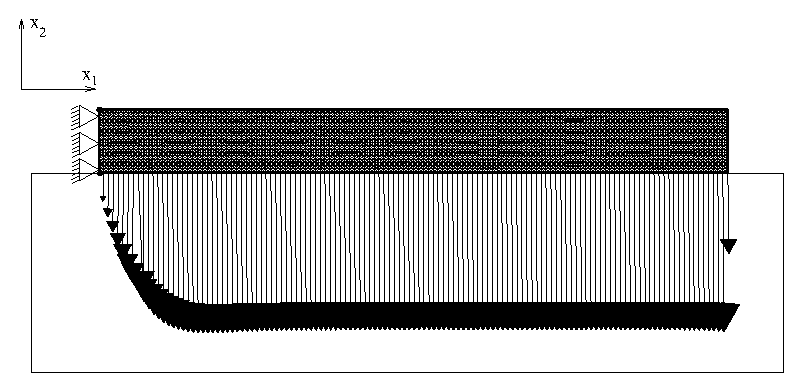
\includegraphics{chapitres/chapitre_2/figures/poutre_def1.eps}}
	\end{center}
		\caption{Configuration déformée de la poutre contre une fondation.}
		\label{poutre_def1}
\end{figure}
%ffffffffffffffffffffffffffffff.
%ffffffffffffffffffffffffffffff
\begin{figure}[ht!]
	\begin{center}
		\resizebox{10cm}{!}{\includegraphics{chapitres/chapitre_2/figures/cont_uniB.eps}}
	\end{center}
	\caption{Contraintes de contact normales sur la zone de contact.}
	\label{cont_uniB}
\end{figure}
%ffffffffffffffffffffffffffffff
%ffffffffffffffffffffffffffffff
\begin{figure}[ht!]
	\begin{center}
		\resizebox{10cm}{!}{\includegraphics{chapitres/chapitre_2/figures/cont_froB.eps}}
	\end{center}
	\caption{Contraintes de frottement tangentielles sur la zone de contact.}
	\label{cont_frotB}
\end{figure}
%ffffffffffffffffffffffffffffff

\noindent\textbf{Précision de la méthode Active Set par rapport à la méthode du quasi-Lagrangien augmenté.}\\

Tout d'abord, nous analysons la précision des contraintes normales et tangentielles de contact avec frottement de la méthode Active Set en la comparant au quasi-Lagrangien augmenté (cf \cite{alart1991mixed}). La frontière $\Gamma_3$ est divisée en 128 parts égales; la contrainte de contact normale $\sigma_{\nu}$ et la contrainte de frottement tangentielle $\|\bsigma_{\tau}\|$ par rapport à l'abscisse sont représentées dans les Figures \ref{cont_uniB} et \ref{cont_frotB} pour chacune des méthodes. Nous noterons que pour $\sigma_{\nu}$ et $\|\bsigma_{\tau}\|$, il n'y a pas de différence visible ($\approx 1\times10^{-7}$), confirmant ainsi la précision sur ce cas de test.\\
Maintenant, nous pouvons comparer l'efficacité des algorithmes mis en oeuvre.\\

\noindent\textbf{Performances des algorithmes}.
Dans la Table \ref{tab1_def}, nous étudions la convergence de la méthode Active Set pour le contact bilatéral associé à la loi de frottement de Tresca en fournissant le nombre de degrés de liberté (ddl), le nombre d'itérations de Newton (Nit) et le temps CPU total en seconde requis pour atteindre la convergence, et ce pour plusieurs valeurs du nombre de noeuds de contact sur la frontière $\Gamma_3$ (nbc). Nous menons la même étude pour la méthode du quasi-Lagrangien augmenté (Table \ref{tab2_def}).
%#######################################################
\begin{table}[htbp!]
\begin{tabular}{ |p{1.25cm}|p{1.25cm}|p{1.25cm}|p{1.25cm}|p{1.25cm}|p{1.25cm}|p{1.25cm}|p{1.25cm}| }
 \hline \rowcolor{lightgray}
 nbc & 8 & 16 & 32 & 64 & 128 & 256 & 512 \\
			\hline
			ddl & 76 & 166 & 586 & 2414 & 10024 & 40528 & 162976 \\
			Nit &  7 & 9 & 9 & 11 & 12 & 13 & 13 \\
			CPU &  $<$1 & $<$1 & $<$1 & 2 & 11 & 70 & 454  \\
 \hline
\end{tabular}
\caption{Résultats de la méthode Active Set pour le contact bilatéral associé à la loi de             frottement de Tresca
	    %(symetric linear systems)
	    en comparaison avec le nombre de degrés de liberté (ddl), le nombre de noeuds de contact (nbc), les itérations de Newton (Nit) et le temps CPU total (CPU) en secondes.}\label{tab1_def}
\end{table}
%#######################################################

%#######################################################
\begin{table}[htbp!]
\begin{tabular}{ |p{1.25cm}|p{1.25cm}|p{1.25cm}|p{1.25cm}|p{1.25cm}|p{1.25cm}|p{1.25cm}|p{1.25cm}| }
 \hline \rowcolor{lightgray}
			nbc & 8 & 16 & 32 & 64 & 128 & 256 & 512 \\
			\hline
			ddl & 92 & 198 & 650 & 2580 & 10280 & 41040 & 164000 \\
			Nit &  5 & 9 & 9 & 11 & 10 & 11 & 9 \\
			CPU &  $<$1 & $<$1 & $<$1 & 5 & 23 & 145 & 807  \\
\hline
\end{tabular}
\caption{Résultats de la méthode du quasi-Lagrangien augmenté pour les lois de contact bilatéral et         de frottement de Tresca
	        %(nonsymetric linear systems)
		     en comparaison avec le nombre de degrés de liberté (ddl), le nombre de noeuds de contact (nbc), les itérations de Newton (Nit) et le temps CPU total (CPU) en secondes.}\label{tab2_def}
\end{table}
%#######################################################
Lorsque $ nbc>64$, la méthode du quasi-Lagrangien augmenté est légèrement plus efficace que la méthode Active Set. Cependant, la méthode Active Set est beaucoup plus rapide en termes de temps CPU que le quasi-Lagrangien, presque deux fois plus rapide. Cela est dû non seulement au fait que la méthode Active Set ne nécessite pas l'utilisation des multiplicateurs de Lagrange mais aussi au fait que la méthode utilise des systèmes linéarisés symétriques, contrairement à la méthode du quasi-Lagrangien augmenté qui présente des sytèmes non-linéarisés symétriques dû au frottement. Cela implique que le système linéaire résultant du problème non-linéaire est plus petit pour la méthode Active Set, comme le confirme la comparaison entre le nombre de degrés de liberté $ddl$ dans les deux cas, et peut être mieux conditionné que le système issu de la méthode du quasi-Lagrangien augmenté, une caractéristique bien connue des problèmes de contact avec frottement.


\subsection{Exemple de contact unilatéral avec frottement de Coulomb}
\label{substatcoulomb}
Dans la configuration $nbc=128$ représentée sur la Figure \ref{poutre_conf2}, 9728 éléments finis élastiques ont été utilisés et le nombre total de degrés de liberté est égal à 10024. Le comportement de l'interaction entre le corps déformable et la fondation est décrit par une loi de contact unilatéral avec la loi de frottement de Coulomb.

Pour le calcul ci-dessous, les données suivantes ont été utilisées:
\begin{eqnarray*}
	\begin{array}{l}
		E= 100N/m^2,\quad \kappa=0.3,\nonumber \\[2mm]
		\fb_0=(0,0) N/m^2, \quad \fb_2= (0,-0.1)\, N/m    \quad \mbox{ sur } 
		\Gamma_2, \nonumber\\[2mm]
		c_\nu=10, \quad c_\tau=10,\quad r_{ lagrangien}=0.1,\quad \mu=0.2, \nonumber\\[2mm]
		{\rm crit\acute{e}re \quad d'arr\hat{e}t}: \epsilon=10^{-6}
	\end{array}
\end{eqnarray*}

Dans la Figure \ref{poutre_def2}, la configuration déformée ainsi que les contraintes de contact normales sur la frontière $\Gamma_3$ sont tracées.\\

%ffffffffffffffffffffffffffffff
\begin{figure}[ht!]
	\begin{center}
		\resizebox{10cm}{!}{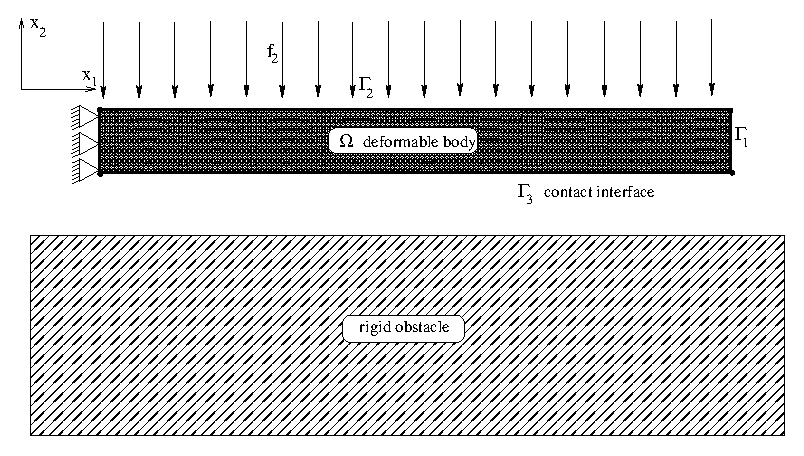
\includegraphics{chapitres/chapitre_2/figures/poutre_conf2.eps}}
	\end{center}
	\caption{Fixation physique de la poutre unilatérale contre une fondation.}
	\label{poutre_conf2}
\end{figure}
%ffffffffffffffffffffffffffffff.

%ffffffffffffffffffffffffffffff
\begin{figure}[ht!]
	\begin{center}
		\resizebox{10cm}{!}{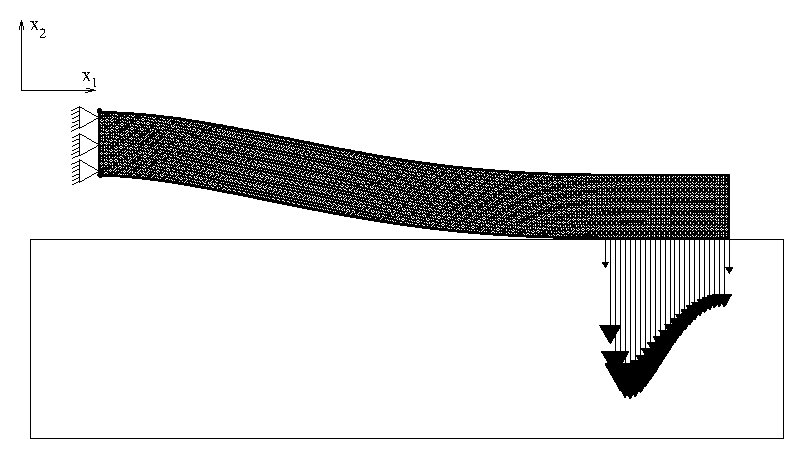
\includegraphics{chapitres/chapitre_2/figures/poutre_def2.eps}}
	 \caption{Configuration déformée de la poutre unilatérale contre une fondation.}
		\label{poutre_def2}
	\end{center}
	
\end{figure}
%ffffffffffffffffffffffffffffff.
\noindent\textbf{Précision de la méthode Active Set par rapport à la méthode du quasi-Lagrangien augmenté.}\\
%ffffffffffffffffffffffffffffff
\begin{figure}[ht!]
	\begin{center}
		\resizebox{10cm}{!}{\includegraphics{chapitres/chapitre_2/figures/cont_uniS.eps}}
	\end{center}
	\caption{Contraintes de contact normales sur la zone de contact.}
	\label{cont_uniS}
\end{figure}
%ffffffffffffffffffffffffffffff
%ffffffffffffffffffffffffffffff
\begin{figure}[ht!]
	\begin{center}
		\resizebox{10cm}{!}{\includegraphics{chapitres/chapitre_2/figures/cont_froS.eps}}
	\end{center}
	\caption{Contraintes de frottement tangentielles sur la zone de contact.}
	\label{cont_frotS}
\end{figure}
%ffffffffffffffffffffffffffffff
Là encore, nous évaluons la précision de la méthode Active Set en la comparant au quasi-Lagrangien augmenté. La frontière $\Gamma_3$ est divisée en 128 parts égales; la contrainte de contact normale $\sigma_{\nu}$ et la contrainte de frottement tangentiel $\|\bsigma_{\tau}\|$ par rapport à l'abscisse sont représentées dans les figures \ref{cont_uniS} et \ref{cont_frotS} pour chacune des méthodes. Encore une fois, il s'avère que pour la contrainte de contact calculée par les deux méthodes, que ce soit $\sigma_{\nu}$ ou $\|\bsigma_{\tau}\|$, il n'y a pas de différence visible ($\approx 1\times10^{-7}$), confirmant ainsi la précision sur ce cas de test.\\

\noindent\textbf{Performances des algorithmes.}\\
Dans la Table \ref{tab3_def}, nous étudions la convergence de la méthode Active Set en fournissant pour le contact unilatéral et la loi de frottement de Coulomb le nombre de degrés de liberté (ddl), le nombre d'itérations de Newton (Nit), le nombre d'itérations de point fixe (fpit) pour approcher la loi de frottement de Coulomb et le temps CPU total (CPU) en seconde requis pour atteindre la convergence, et ce pour plusieurs valeurs du nombre de noeuds de contact sur la frontière $\Gamma_3$ (nbc). Nous menons la même étude pour la méthode du quasi-Lagrangien augmenté pour la loi de contact unilatéral et de frottement de Coulomb (Table \ref{tab4_def}).\\
Dans ce cas, contrairement à la configuration avec contact bilatéral, le nombre d'itérations de Newton n'est plus approprié pour comparer les deux méthodes, car la méthode Active Set approche le frottement de Coulomb avec une boucle interne supplémentaire impliquant une succession d'états de frottement de Tresca tandis que la méthode du quasi-Lagrangien augmenté ne fait pas d'approximation. Par conséquent, le seul critère fiable disponible est le temps CPU. Malgré cette boucle supplémentaire, sur les deux méthodes, la méthode Active Set reste la plus rapide. Lorsque $ nbc = 512 $, l'écart entre les deux méthodes augmente avec le nombre de degrés de liberté. Une telle hypothèse doit être confirmée pour des problèmes plus complexes.\\
%#######################################################
\begin{table}[htbp!]
\begin{tabular}{ |p{1.25cm}|p{1.25cm}|p{1.25cm}|p{1.25cm}|p{1.25cm}|p{1.25cm}|p{1.25cm}|p{1.25cm}| }
 \hline \rowcolor{lightgray}
			nbc & 8 & 16 & 32 & 64 & 128 & 256 & 512 \\
			\hline
			ddl & 76 & 166 & 586 & 2414 & 10024 & 40528 & 162976 \\
			Nit &  15 & 25 & 37 & 45 & 44 & 46 & 39 \\
            fpit &  5 & 5 & 5 & 5 & 5 & 5 & 7 \\
			CPU &  $<$1 & $<$1 & 1 & 9 & 61 & 364 & 1448  \\
\hline
\end{tabular}
\caption{Résultats de la méthode Active Set pour les lois de contact unilatéral et de               frottement de Tresca %(fixed point method - symetric linear systems)
		   en comparaison avec le nombre de degrés de liberté (ddl), le nombre de noeuds de contact (nbc), les itérations de Newton (Nit), les itérations de point fixe (fpit) et le temps CPU total (CPU) en secondes.}\label{tab3_def}
\end{table}
%#######################################################

%#######################################################
\begin{table}[htbp!]
\begin{tabular}{ |p{1.25cm}|p{1.25cm}|p{1.25cm}|p{1.25cm}|p{1.25cm}|p{1.25cm}|p{1.25cm}|p{1.25cm}| }
 \hline \rowcolor{lightgray}
			nbc & 8 & 16 & 32 & 64 & 128 & 256 & 512 \\
			\hline
			ddl & 92 & 198 & 650 & 2580 & 10280 & 41040 & 164000 \\
			Nit &  4 & 17 & 20 & 23 & 26 & 27 & 28 \\
			CPU &  $<$1 & $<$1 & 1 & 9 & 62 & 405 & 2972  \\
\hline
\end{tabular}
	\caption{Résultats de la méthode du quasi-Lagrangien augmenté pour les lois de contact unilatéral et de frottement de Coulomb en comparaison avec le nombre de degrés de liberté (ddl), le nombre de nœuds de contact (nbc), les itérations de Newton (Nit) et le temps CPU total (CPU) en secondes.} \label{tab4_def}
\end{table}
%#######################################################

\section{Simulations numériques dans le cas dynamique}\label{simu_dynam}

Après avoir évalué les performances et la précision des méthodes Active Set implémentées sur des cas statiques simples, notre objectif désormais est d'évaluer la robustesse de ces méthodes sur des problèmes plus complexes. Les simulations dans cette partie sont réalisées à partir de deux configurations de contact dynamique: le contact unilatéral avec la loi de frottement de Coulomb d'une poutre élastique linéaire sur une fondation rigide, puis le rebond d'un anneau hyper-élastique contre une fondation rigide. La solution numérique du problème ${\cal P}$ est calculée par les méthodes Active Set et quasi-Lagrangien augmenté afin de mettre en évidence les performances de la première méthode par rapport à la seconde.
Comme pour les exemples numériques de la section précédente, le domaine $\Omega$ représente la section transversale d'un corps déformable tridimensionnel soumis à l'action de la vitesse initiale de telle sorte qu'une hypothèse de contrainte plane est supposée.


\subsection{Exemple académique: compression d'une poutre contre une fondation rigide}

La configuration de référence est la même que celle introduite dans la sous-section \ref{substatcoulomb}.

Pour le calcul ci-dessous, les données suivantes ont été utilisées:
\begin{eqnarray*}
	\begin{array}{l}
		\rho = 1000kg/m^3, \quad T=0.5s,  \quad k=\frac{1}{10}, \nonumber \\[2mm]
		E= 10N/m^2,\quad \kappa=0.3,\nonumber \\[2mm]
		\fb_0=(0,0) N/m^2, \quad \fb_2= (0,-0.1)\, N/m    \quad \mbox{ sur }
		\Gamma_2, \nonumber\\[2mm]
		c_\nu=10, \quad c_\tau=10,\quad r_{lagrangien}=0.1\nonumber, \quad \mu = 0.2\\[2mm]
		{\rm crit\acute{e}re \quad d'arr\hat{e}t}: \epsilon=10^{-6}.
	\end{array}
\end{eqnarray*}

\noindent\textbf{Précision de la méthode Active Set par rapport à la méthode du quasi-Lagrangien augmenté dans le cas dynamique.}\\
Nous allons à présent évaluer la précision de la méthode Active Set en la comparant au quasi-Lagrangien augmenté dans le cas dynamique. La frontière  $\Gamma_3$ est divisée en $128$ parts égales; la contrainte de contact normale $\sigma_{\nu}$ et la contrainte de frottement tangentiel $\|\bsigma_{\tau}\|$ par rapport à l'abscisse sont représentées dans les Figures \ref{cont_uniD} et \ref{cont_froD} pour chacune des méthodes. Nous constatons ainsi qu'il n'y a aucune différence entre la contrainte de contact calculée par les deux méthodes.\\

%%ffffffffffffffffffffffffffffff

\begin{figure}[ht!]
            \begin{center}
                   \resizebox{10cm}{!}{\includegraphics{chapitres/chapitre_2/figures/cont_uniD.eps}}
            \end{center}
            \caption{Contraintes de contact normales sur la zone de contact.}
            \label{cont_uniD}
\end{figure}

%%ffffffffffffffffffffffffffffff
%%ffffffffffffffffffffffffffffff

\begin{figure}[ht!]
            \begin{center}
                      \resizebox{10cm}{!}{\includegraphics{chapitres/chapitre_2/figures/cont_froD.eps}}
            \end{center}
            \caption{Contraintes de frottement tangentielles sur la zone de contact.}
            \label{cont_froD}
\end{figure}
%%ffffffffffffffffffffffffffffff

\noindent\textbf{Performances des algorithmes.}\\
Pour cet exemple, la méthode Active Set fonctionne mieux que la méthode du quasi-Lagrangien augmenté uniquement lorsque $ nbc> 512 $ (voir Table \ref{tab5_def} et \ref{tab6_def}). Cependant, d'après la Figure \ref{dynaelas_CPU}, plus le nombre de noeuds de contact est grand, plus l'écart de temps CPU entre les méthodes croît, rendant ainsi la méthode Active Set plus pertinente.

%#######################################################
\begin{table}[htbp!]
\begin{tabular}{ |p{1.25cm}|p{1.25cm}|p{1.25cm}|p{1.25cm}|p{1.25cm}|p{1.25cm}|p{1.25cm}|p{1.25cm}| }
 \hline \rowcolor{lightgray}
			nbc & 8 & 16 & 32 & 64 & 128 & 256 & 512 \\
			\hline
			ddl & 76 & 166 & 586 & 2414 & 10024 & 40528 & 162976 \\
			Ntit &  119 & 153 & 191 & 254 & 258 & 240 & 216 \\
			afpit &  4 & 4 & 4 & 4 & 5 & 4 & 5 \\
			CPU &  0.07 & 0.33 & 2.52 & 25.57 & 162.28 & 861.92 & 3295.57  \\
\hline
\end{tabular}
	\caption{Résultats de la méthode Active Set pour le contact unilatéral et frottement de Coulomb en comparaison avec le nombre de degrés de liberté (ddl), le nombre de noeuds de contact (nbc), le nombre total d'itérations de Newton (Ntit), de point fixe moyen (afpit) et le temps CPU total (CPU) en secondes.} \label{tab5_def}
\end{table}
%#######################################################

%#######################################################
\begin{table}[htbp!]
\begin{tabular}{ |p{1.25cm}|p{1.25cm}|p{1.25cm}|p{1.25cm}|p{1.25cm}|p{1.25cm}|p{1.25cm}|p{1.25cm}| }
 \hline \rowcolor{lightgray}
			nbc & 8 & 16 & 32 & 64 & 128 & 256 & 512 \\
			\hline
			ddl & 92 & 198 & 650 & 2580 & 10280 & 41040 & 164000 \\
			Ntit &  37 & 58 & 80 & 87 & 98 & 112 & 119 \\
			CPU &  0.04 & 0.28 & 2.25 & 20.05 & 113.78 & 769.38 & 5773.57  \\
\hline
\end{tabular}
	\caption{Résultats de la méthode du quasi-Lagrangien augmenté pour le contact unilatéral et frottement de Coulomb en comparaison avec le nombre de degrés de liberté (ddl), le nombre de nœuds de contact (nbc), le nombre total d'itérations de Newton (Ntit) et le temps CPU total (CPU) en secondes.} \label{tab6_def}
\end{table}
%#######################################################

\begin{figure}[ht!]
	\begin{center}
		\resizebox{10cm}{!}{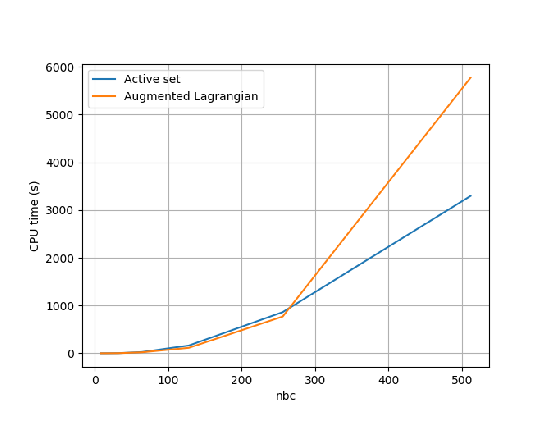
\includegraphics{chapitres/chapitre_2/figures/dynaelas}}
	\end{center}
	\caption{Temps CPU pour les méthodes Active Set et quasi-Lagrangien augmenté en fonction de $ nbc $.}
	\label{dynaelas_CPU}
\end{figure}
%ffffffffffffffffffffffffffffff

\subsection{Exemple pertinent: rebond d'un anneau hyper-élastique contre une fondation rigide}
%ffffffffffffffffffffffffffffff
\begin{figure}[!h]
	\begin{center}
			\resizebox{10cm}{!}{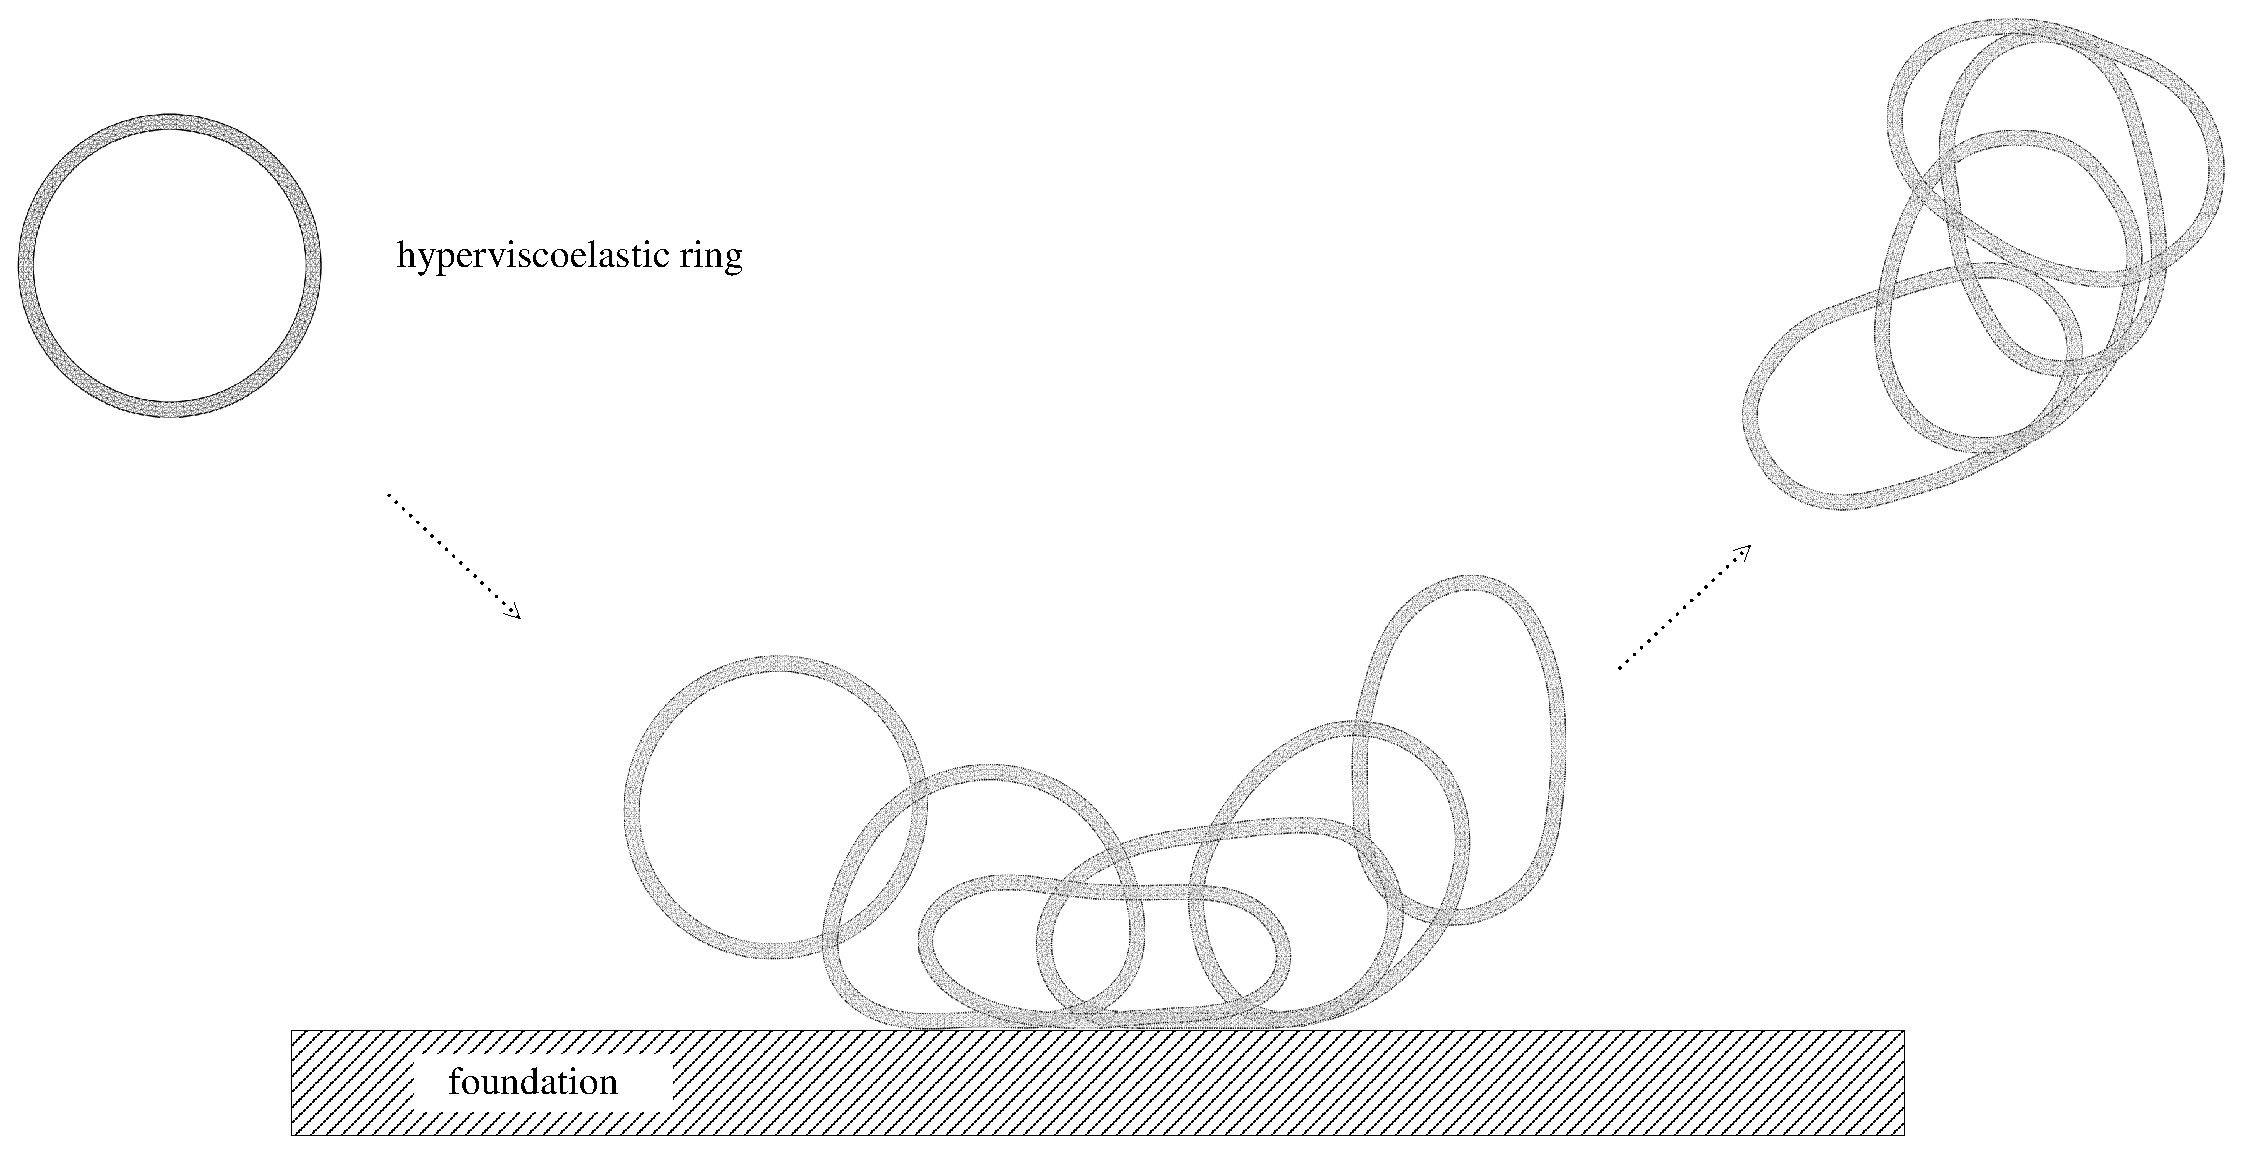
\includegraphics{chapitres/chapitre_2/figures/ring_sequence}}
	\end{center}
	\caption{Séquence de l'anneau hyper-élastique déformé avant, pendant et après l'impact.}
	\label{ring_test}
\end{figure}
%ffffffffffffffffffffffffffffff
Nous considérons maintenant une deuxième application représentative afin d'évaluer les performances des méthodes types Active Set dans le cas d'un cadre en grandes déformations. Il s'agit d'un exemple plus pertinent que les exemples précédents de problème de contact avec frottement.\\
Pour la discrétisation, nous choisissons un paramètre $ nbc $ décrivant le nombre de nœuds de contact sur $ \Gamma $ (le nombre de noeuds sur le contour extérieur de l'anneau est donc pris afin d'obtenir des éléments suffisamment réguliers) . Dans la configuration $ nbc = 128 $ représentée sur la Figure \ref{ring_test}, la frontière $\Gamma_3$ est divisée en 128 parts égales, 1664 éléments finis hyper-élastiques ont été utilisés pour un nombre total de degrés de liberté égal à 2048.
La réponse du matériau compressible, considérée ici, est régie par une variante de la loi de comportement d'Ogden (cf \cite{ciarlet1982lois}) définie par la densité d'énergie suivante


%
%%%%%%%%%%%%%%%%%%%%%%%%%
\begin{equation}\nonumber
W({\bf C}) = c_1 (I_1 - 3) + c_2 (I_2 - 3) + a (I_3 - 1) - (c_1 + 2 c_2 + a) \ln
I_3.
\end{equation}
%%%%%%%%%%%%%%%%%%%%%%%%%%%%%
\noindent Ici $I_1, I_2$ et $I_3 $ représentent les trois invariants
du tenseur de Cauchy ${\bf C}$, avec ${\bf C} = {\bf F}^{\bf T} {\bf F}$. 

Les détails sur la configuration physique du problème sont donnés ci-dessous. Le domaine $ \Omega $ est défini par:
\begin{align*}
\Omega\, &=\left\{(x_1,x_2)\in \mathbb{R}^2:  \ 81 <(x_1-100)^2
+ (x_2-100)^2 \leq 100 \right\},\\
\Gamma_1&=  \varnothing, \qquad \Gamma_2=  \varnothing,\\
\Gamma_3&=\left\{(x_1,x_2)\in \mathbb{R}^2: \ (x_1-100)^2
+ (x_2-100)^2 = 100 \right\}.
\end{align*}

Le domaine $ \Omega $ représente la section d'un corps déformable tridimensionnel sous l'hypothèse de contrainte plane. L'anneau est projeté avec une vitesse initiale à un angle de $45^o$ vers une fondation comme le montre la Figure \ref{ring_test}. La fondation est donnée par $\left\{(x_1,x_2)\in \mathbb{R}^2:  \ x_2 \leq 0  \right\}$. Pour la discrétisation, nous utilisons 1664 noeuds élastiques et 128 noeuds de contact. Pour les expériences numériques, les données sont:
\begin{eqnarray}
\begin{array}{l}
\rho = 1000 kg/m^3, \quad T=5s,  \quad k=\frac{1}{500}, \nonumber \\[2mm]
\bu_0=(0,0) m,  \quad \bu_1=(10,-10) m/s, \nonumber \\[2mm]
c_1 = 0.5 MPa, \quad c_2 = 0.05 MPa, \quad a = 0.5x10^{-4} MPa,  \nonumber \\[2mm]
c_\nu=10, \quad c_\tau=10,\quad r_{lagrangien}=0.1\nonumber\\[2mm]
g=50\,m,  \quad \mu = 0.2, \nonumber \\[2mm]
{\rm crit\acute{e}re \quad d'arr\hat{e}t}: \epsilon=10^{-6}.
\end{array}
\end{eqnarray}

Comme dans la section précédente, nous comparons les résultats obtenus par la méthode Active Set et la méthode du quasi-Lagrangien augmenté en ce qui concerne la convergence et les performances des méthodes (voir Tables \ref{tab7_def} et \ref{tab8_def}). 
%#######################################################
\begin{table}[htbp!]
\begin{tabular}{ |p{1.8cm}|p{1.8cm}|p{1.8cm}|p{1.8cm}|p{1.8cm}|p{1.8cm}| }
 \hline \rowcolor{lightgray}
			nbc  & 32 & 64 & 128 & 256 & 512 \\
			\hline
			ddl & 192 & 384 & 1792 & 4608 & 15360  \\
			Ntit &  1876 & 1904 & 1944 & 1961 & 2022  \\
			afpit &  4 & 4 & 4 & 4 & 4  \\
			CPU &  6.32 & 12.39 & 99.22 & 304.62 & 1841.23   \\
\hline
\end{tabular}
	\caption{Résultats de la méthode Active Set pour les lois de contact unilatéral et de frottement de Coulomb en comparaison avec le nombre de degrés de liberté (ddl), le nombre de noeuds de contact (nbc), le nombre total d'itérations de Newton (Ntit), de point fixe moyen (afpit) et le temps CPU total (CPU) en secondes.} \label{tab7_def}
\end{table}
%#######################################################

%#######################################################
\begin{table}[htbp!]
\begin{tabular}{ |p{1.8cm}|p{1.8cm}|p{1.8cm}|p{1.8cm}|p{1.8cm}|p{1.8cm}| }
 \hline \rowcolor{lightgray}
			nbc  & 32 & 64 & 128 & 256 & 512 \\
			\hline
			ddl & 256 & 512 & 2048 & 5120 & 16384  \\
			Ntit &  1462 & 1568 & 1705 & 1782 & 1866  \\
			CPU &  8.59 & 18.03 & 139.69 & 428.80 & 2693.86   \\
\hline
\end{tabular}
	\caption{Résultats de la méthode du quasi-Lagrangien augmenté pour les lois de contact unilatéral et de frottement de Coulomb en comparaison avec le nombre de degrés de liberté (ddl), le nombre de nœuds de contact (nbc), le nombre total d'itérations de Newton (Ntit) et le temps CPU total (CPU) en quelques secondes.} \label{tab8_def}
\end{table}
%#######################################################

Bien que ce cas soit assez complexe, les performances de la méthode Active Set s'améliorent. D'après la Figure \ref{dynahyper_CPU}, plus le nombre de noeuds de contact est grand, plus l'écart de temps CPU entre les méthodes s'élargit, ce qui est cohérent avec notre hypothèse de la partie précédente, et confirme la robustesse de ces méthodes sur des configurations complexes. Cependant, cela ne suffit pas pour expliquer le gain en temps CPU de la méthode Active Set approchée par rapport à la méthode du quasi-Lagrangien augmenté. Comme mentionné à la fin de la section \ref{fullcoulombactive}, les systèmes linéarisés sont symétriques, même en cas de frottement, alors qu'ils ne le sont pas pour le quasi-Lagrangien. Ainsi, la symétrie des systèmes linéarisés et l'absence des multiplicateurs de Lagrange sont des arguments pertinents et solides en faveur des méthodes types Active Set. 

\begin{figure}[h!]
	\begin{center}
		\resizebox{10cm}{!}{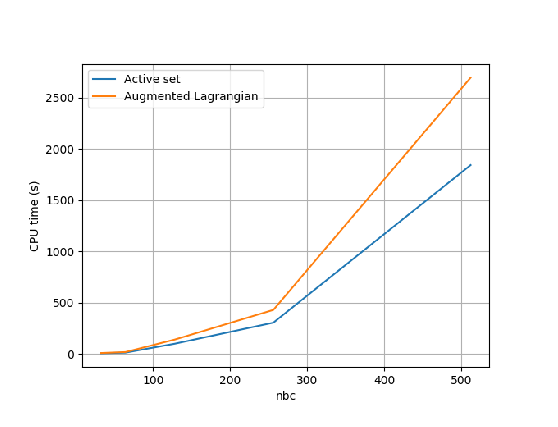
\includegraphics{chapitres/chapitre_2/figures/dynahyper.eps}}
	\end{center}
	\caption{Temps CPU pour la méthode Active Set et le quasi-Lagrangien augmenté en fonction de $nbc$.}
	\label{dynahyper_CPU}
\end{figure}
%ffffffffffffffffffffffffffffff

Cet exemple montre clairement la robustesse de la méthode Active Set dans une configuration complexe. Il semble que l'absence des multiplicateurs de Lagrange reste un argument solide pour choisir la méthode Active Set plutôt que la méthode du quasi-Lagrangien augmenté pour la résolution numérique de ce genre de problèmes de contact.




 
\section{Compléments des méthodes de type Active Set sur les conditions de contact persistant}\label{complement_persistant}

Nous présentons dans cette section quelques compléments numériques sur les méthodes de type Active Set dans le cadre d'un contact persistant. D'ailleurs, cette partie servira de transition avec le chapitre suivant car une telle loi permet de conserver l'énergie durant le contact. Pour illustrer cela, nous considérons le cas d'une balle élastique linéaire qui rebondit sur une fondation rigide pour laquelle nous étudions la séquence de déformation au cours du temps ainsi que les forces de contacts qui s'y exercent dessus avant, pendant et après l'impact.  

\subsection{Conditions de contact persistants}\label{cont_cond}

Lorsqu'un contact ponctuel a lieu entre une balle élastique linéaire (solide déformable) et une fondation rigide, une force de répulsion normale qui vérifie les conditions de Signorini est exercée au point de contact. L'énergie fournie par cette force est alors conservée (voir \cite{laursen2013computational}, \cite{laursen1997design}) sous réserve qu'une condition de persistence (\ref{pers_not_gap_2}) s'ajoute aux conditions de contact unilatéral (\ref{pers_gap})--(\ref{pers_not_gap_1}). Cette condition signifie qu'il ne peut y avoir d'impulsion normale de contact que lorsque celle-ci est persistente. Par ailleurs, si un frottement sec est pris en compte, il introduit une relation entre l'impulsion de contact et la vitesse relative locale de la balle élastique. Les conditions de contact et de frottement sont alors basées sur la combinaison des conditions de contact unilatéral  exprimées en vitesse avec une loi de Coulomb de frottement sec. L'ajout de la condition de persistence aux conditions de contact unilatéral (voir preuve dans \cite{laursen2013computational}, \cite{moreau1994numerical} et \cite{moreau1999sweeping}) permet d'écrire:

\begin{eqnarray}  
&\mbox{si} \ \ d_{\nu} > 0  \quad & \lambda_{\nu} = 0 \ ;\ \blambda_{\tau} =0  \label{pers_gap} \\
&\mbox{si} \ \ d_{\nu} = 0  \quad & \\ 
&&\dot u_{\nu} \ge 0 \label{pers_not_gap},\\
&&\lambda_{\nu}\ge 0 \label{pers_not_gap_1},\\
&&\dot u_{\nu}\lambda_{\nu}= 0 \label{pers_not_gap_2},\\
&& \left\{\begin{array}{ll} \label{pers_not_gap_coulomb}
\|\blambda_{\tau}\|\le\,\mu |\lambda_{\nu}|,\\[2mm]
\|\blambda_{\tau}\|<\,\mu |\lambda_{\nu}|\Longrightarrow \dot\bu_{\tau}=0,\\[2mm]
\|\blambda_{\tau}\|=\,\mu |\lambda_{\nu}|\Longrightarrow \exists \beta\ge 0: \blambda_{\tau}=\beta \dot\bu_{\tau}, \end{array}\right .
 \end{eqnarray}
 
$g$ étant la distance minimale autorisée (interstice) entre un point de la surface de contact et sa projection sur la fondation rigide. La loi de frottement de Coulomb (\ref{pers_not_gap_coulomb}) dépend de la contrainte de  frottement  tangentielle $\blambda_{\tau}$,  de  la  pression  de  contact  normale  $\lambda_{\nu}$ et de la  vitesse  de  contact tangentielle $\dot\bu_{\tau}$.

\subsection{Méthode de type "Primal-dual Active Set"}\label{Activeset_type}

Les conditions de contact unilatéral avec frottement dans le cadre d'un contact persistant (\ref{pers_gap})--(\ref{pers_not_gap_coulomb}) sont réalisées en appliquant une stratégie Active Set sur les fonctions de complémentarité non-linéaires ${\cal R}_{\nu}^{\blambda}$ et ${\cal R}_{\tau}^{\blambda}$ basées sur un formalisme itératif de Newton semi-régulier. Les ensembles actifs et inactifs sont définis selon un schéma de point milieu "\textit{leapfrog}" défini comme suit:

\begin{align*}
&d_{\nu}^{leapfrog} = d_{\nu,p} + \frac{\Delta{t}}{2} \dot u_{\nu,p},
\end{align*}

\noindent avec $\dot u_{\nu,p} = \frac{u_{\nu,p}-u_{\nu,p-1}}{\Delta{t}}$. Le statut d'un noeud donné à l'itération $k$ dépend de l'ensemble auquel il appartient; sur la base des parties précédentes, il peut être à l'état sans contact, avec contact glissant ou avec contact adhérant.\\

\noindent La description de l'algorithme itératif Active Set d'indice $k$ dans le cadre d'un contact persistant est la suivante:\\

\noindent (i) \quad Choisir $(\bu^{(0)},\blambda^{(0)})$, $c_{\nu}>0$, $c_\tau>0$ et initialiser $k=0$.\\[3mm]
\qquad(ii) \quad si \ $d_{\nu}^{leapfrog} > 0$ \qquad  $\lambda^{(k)}_{\nu,p} = 0$ \ ;\ $\blambda_{\tau, p}^{(k)} =0$ \\[3mm]
\qquad(iii) \quad si \ $d_{\nu}^{leapfrog} \le 0$  \qquad les ensembles actifs et inactifs:
\begin{align*}
&{\cal A}_{\nu}^{k+1}=\{p\in {\cal S}:\lambda^{(k)}_{\nu,p}+c_{\nu} \dot u^{(k)}_{\nu,p}> 0\},\\
&{\cal I}_{\nu}^{k+1}={\cal S}\setminus {\cal A}_{\nu}^{k+1},\\
&{\cal A}_{\tau}^{k+1}=\{p\in {\cal S}:\|\blambda_{\tau, p}^{(k)}+c_\tau \dot\bu_{\tau, p}^{(k)}\|-\mu \lambda_{\nu, p}^{(k)}> 0\},\\
&{\cal I}_{\tau}^{k+1}={\cal S}\setminus {\cal A}_{\tau}^{k+1}.
\end{align*}
(iv) Trouver $(\bu^{(k+1) },\blambda^{(k+1) })$ tel que
\begin{eqnarray}
& \rho \ddot{\bu}^{(k+1)}+ A(\bu^{(k+1)}) + \lambda_{\nu}^{(k+1)}\nu + \blambda_{\tau}^{(k+1)}= \fb, \\[1mm]
&\label{Anu}\dot u^{(k+1)}_{\nu,p}=0 \quad {\rm pour \ tout} \quad p\in {\cal A}_{\nu}^{k+1},\\[1mm]
&\label{Inu}\lambda^{(k+1)}_{\nu,p}=0, \quad \blambda^{(k+1)}_{\tau,p}=\bzero \quad {\rm pour \ tout} \quad p\in {\cal I}_{\nu}^{k+1},\\[1mm]
&\label{Atau}\blambda_{\tau, p}^{(k+1)} = \mu \lambda_{\nu, p}^{(k+1)} \frac{\blambda_{\tau, p}^{(k)}+c_\tau \dot\bu_{\tau, p}^{(k)}}{\|\blambda_{\tau, p}^{(k)}+c_\tau \dot\bu_{\tau, p}^{(k)}\|} \quad {\rm pour \ tout} \ p\in {\cal A}_{\tau}^{k+1}\cap {\cal A}_{\nu}^{k+1},\\[1mm]
&\label{Itau}\dot\bu_{\tau, p}^{(k+1)}+\frac{\dot\bu_{\tau, p}^{(k)}}{\lambda_{\nu, p}^{(k)}}\lambda_{\nu, p}^{(k+1)} =\dot\bu_{\tau, p}^{(k)} \quad {\rm pour \ tout} \ p\in {\cal I}_{\tau}^{k+1}\cap {\cal A}_{\nu}^{k+1}.
\end{eqnarray}
(v) Si $\|(\bu^{(k+1) },\blambda^{(k+1)})-(\bu^{(k) },\blambda^{(k)})\|\leq\epsilon$, $\|{\cal R}(\bu^{(k+1) },\blambda^{(k+1)})\|\leq\epsilon$, ${\cal A}_{\nu}^{k+1}={\cal A}_{\nu}^{k}$ et ${\cal A}_{\tau}^{k+1}={\cal A}_{\tau}^{k}$ alors stop, sinon retourner à (ii).\\[1mm]

\subsection{Impact d'une balle élastique linéaire contre une fondation} \label{num_ex1}
Ce problème de référence représentatif décrit l'impact sans frottement d'une balle élastique linéaire contre une fondation (voir \cite{khenous2006discretization}). 
La balle élastique est lancée avec une vitesse initiale ($\bu_1=(0,-10) m/s$) vers la fondation\\
$\left\{(x_1,x_2)\in \mathbb{R}^2:  \ x_2 \leq 0 \right\}$. Le comportement du matériau est décrit par une loi de comportement linéaire élastique définie par la densité d'énergie:

\begin{equation}
	W^e(\bvarepsilon)=\frac{E\kappa}{2(1+\kappa)(1-2\kappa)} (tr
	\bvarepsilon)^2 +\frac{E}{2(1+\kappa)} tr(\bvarepsilon^2), \quad \forall
	\epsilon \in \mathbb{M}^n.
\end{equation}

Ici, $E$ et $\kappa$ sont le module de Young et le rapport de Poisson du matériau et $tr(\cdot)$ désigne la fonction trace, respectivement. Notez que $\bvarepsilon = \frac{1}{2} ({\nabla \bu}^T + \nabla \bu)$ représente le tenseur de déformation linéarisé dans le cadre de la théorie des petites déformations ($\|\bu\|<< 1$ et $\|\nabla \bu\| << 1$ dans $\Omega$).

%%%%%%%%%%%%%%%%%%%%%%%%%%%%%%%%%%%%%%%%%%%%%%%%%%%%%%%%%%%%%%%%%%%%%%%%%%%%%%
\begin{figure}[!h]
	\begin{center}
		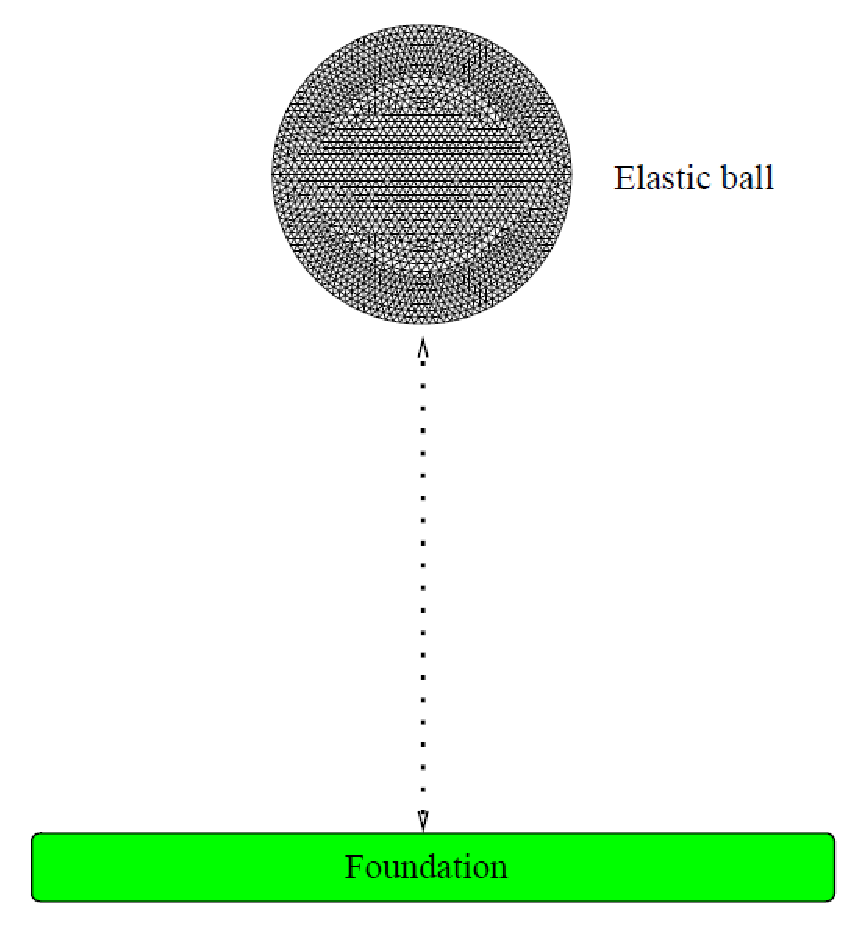
\includegraphics[width=6cm]{chapitres/chapitre_2/figures/ex_num.eps}
	\end{center}
	\caption{Discrétisation de la balle élastique au contact d'une fondation.}
	\label{fig_num1}
\end{figure}
%%%%%%%%%%%%%%%%%%%%%%%%%%%%%%%%%%%%%%%%%%%%%%%%%%%%%%%%%%%%%%%%%%%%%%%%%%%%%%
Le cadre physique est illustré dans la Figure \ref{fig_num1}.
\begin{align*}
\Omega\, &=\left\{(x_1,x_2)\in \mathbb{R}^2:  \ (x_1-100)^2
+ (x_2-100)^2 \leq 100 \right\},\\
\Gamma_1&=  \varnothing, \qquad \Gamma_2=  \varnothing,\\
\Gamma_3&=\left\{(x_1,x_2)\in \mathbb{R}^2: \ (x_1-100)^2
+ (x_2-100)^2 = 100 \right\}.
\end{align*}
Le domaine $\Omega$ représente la section transversale de la balle, sous l'hypothèse de la contrainte plane. Aucune force volumique n'est supposée agir sur le corps pendant le processus. Pour la discrétisation du problème de contact représenté, nous utilisons 7820 noeuds élastiques et 128 noeuds multiplicateurs de Lagrange. Pour les expériences numériques, nous utilisons les données suivantes:
\begin{eqnarray}
\begin{array}{l}
\rho = 1000 kg/m^3, \quad T=2s,  \quad k=0.001, \nonumber \\[2mm]
\bu_0=(0,0) m,  \quad \bu_1=(0,-10) m/s, \nonumber \\[2mm]
E= 100 GPa,\quad \kappa=0.35, \quad \fb_0=(0,0) Pa,  \nonumber \\[2mm]
g=50\,m, \quad c_{\nu} = c_{\tau} = 10, \quad \mu = 0. \nonumber
\end{array}
\end{eqnarray}
%%%%%%%%%%%%%%%%%%%%%%%%%%%%%%%%%%%%%%%%%%%%%%%%%%%%%%%%%%%%%%%%%%%%%%%%%%%%%%

Dans la Figure \ref{defcont}, la séquence de la balle déformée
ainsi que les forces de contact sont présentées avant, pendant et
après l'impact.\\
%%%%%%%%%%%%%%%%%%%%%%%%%%%%%%%%%%%%%%%%%%%%%%%%%%%%%%%%%%%%%%%%%%%%%%%%%%%%%%
\begin{figure}[!h]
	\begin{center}
		\includegraphics[width=11.5cm]{chapitres/chapitre_2/figures/def.eps}
	\end{center}
	\caption{Séquence de la balle déformée et des forces de contact avant, pendant et après l'impact.}\label{defcont}
\end{figure}
%%%%%%%%%%%%%%%%%%%%%%%%%%%%%%%%%%%%%%%%%%%%%%%%%%%%%%%%%%%%%%%%%%%%%%%%%%%%%%
L'intérêt de cet exemple représentatif est de comparer les résultats numériques de la méthode Active-Set obtenus en utilisant certaines méthodes classiques. À cette fin, nous considérons cinq méthodes existantes: 
\begin{itemize}
    \item La méthode quasi-Lagrangien augmenté classique avec condition de contact de Signorini ($r_{lagrangien} = 0.1$).
    \item La méthode de pénalisation avec une condition de compliance normale ${\xi_{{\boldsymbol \nu}}}_{n} = - r _p({u}_{{\boldsymbol \nu}_{n}})_+$ ($r_{p\acute{e}nalisation} = 10^5$).
    \item La méthode de pénalisation spécifique développée par Hauret, Le Tallec {\it et. al} (\cite{ayyad2009formulation}, \cite{hauret2006energy}).
    \item La méthode EMM (Equivalent Mass Matrix) proposée par Khenous {\it et. al} \cite{khenous2006discretization}, qui représente une distribution spécifique de la matrice des masses sans inertie des noeuds de contact. Cette méthode est caractérisée par des propriétés de stabilité pertinentes de la contrainte de contact.
    \item La méthode de continuation de Newton spécifique développée par Ayyad et Barboteu (\cite{ayyad2009formulation}, \cite{barboteu2015hyperelastic}), qui se caractérise par l'application suivant deux étapes de la loi de contact unilatéral et la condition de persistance à chaque incrément de temps.
\end{itemize} 

\vspace*{0.5cm}
%ffffffffffffffffffffffffffffff
\begin{figure}[!h]
	\begin{center}
		\includegraphics[width=15cm]{chapitres/chapitre_2/figures/ene_fr_po_2020.eps}
	\end{center}
	\caption{Comportement énergétique discret de schémas d'intégration temporelle sélectionnés pendant l'impact.}
	\label{ene_ball}
\end{figure}
%ffffffffffffffffffffffffffffff
Dans ce qui suit, nous analysons les méthodes en termes d'évolution d'énergie discrète. À cette fin, l'énergie discrète totale à l'instant $t_{n}$ est définie par la formule suivante:
$$
E_{n} =   \frac{1}{2} \int_{\Omega} \rho \dot{\bu}^{2}_{n} d\bx +
\int_{\Omega} {\boldsymbol \sigma}^e_{n} :
\bvarepsilon(\bu_{n}) d\bx,
$$
où ${\boldsymbol \sigma}^e= \frac{\partial W^e(w)}{\partial \bvarepsilon}$ désigne le tenseur de contrainte pour les déformations infinitésimales.\\
La Figure  \ref{ene_ball} représente l'évolution de l'énergie discrète totale du système dynamique. On note qu'après l'impact (i.e. pour $t \ge 1.52 $) et pour le pas de temps considéré $ k = 0.001 $, la méthode classique avec la loi de Signorini (courbe ( $\circleddash $)) ainsi que la méthode avec condition de compliance normale standard (courbe ($\boxminus$)) se caractérisent par une non conservation de l'énergie, ce qui n'est pas réaliste du point de vue physique. On remarque également que la méthode EMM (courbe $\blacktriangledown$) réduit fortement la dissipation de l'énergie, sans obtenir la conservation exacte. De plus, les schémas développés par Ayyad et Barboteu \cite{ayyad2009formulation}
(courbe ({\Large\textbullet})) et la méthode spécifique pénalisée (courbe ($\blacksquare$)) conservent l'énergie après l'impact. Cependant, pour la méthode pénalisée, nous trouvons des fluctuations d'énergie qui disparaissent après l'impact. De plus, tant pour cette méthode que pour la méthode utilisée dans \cite{ayyad2009formulation}
, le contact unilatéral n'est pas exactement satisfait. En effet, la méthode spécifique pénalisée génère une erreur maximale sur le déplacement de contact normal de $0,0034m$, et $0,0051m$ pour la méthode d'Ayyad et Barboteu \cite{ayyad2009formulation}. La méthode Active Set pour le contact persistant (illustrée par la courbe ($\blacklozenge$)) permet de conserver exactement l'énergie sans aucune fluctuation. En raison du prédicteur du pas de temps "leapfrog", cette méthode Active Set génère une erreur maximale sur le déplacement de contact normal de $0,01540 m$.\\

\vspace{1.5cm}

\section*{Conclusion}

Ce chapitre fournit l'analyse de plusieurs méthodes Active Set à travers les problèmes classiques qui se posent en mécanique des contacts, c'est-à-dire les contacts unilatéraux / bilatéraux associés à la loi de frottement de Tresca / Coulomb en petite et grande déformation. Premièrement, nous avons dérivé une formulation variationnelle du problème mécanique avec une approximation numérique du problème. Après cela, nous avons présenté plusieurs méthodes de type Active Set, rappelant celle introduite dans \cite{abide2016analysis} dans le cas sans frottement et en l'étendant au cas du contact bilatéral avec la loi de frottement de Tresca puis au cas unilatéral avec la loi de frottement de Coulomb avec leur algorithmes. Nous considérons également une alternative pour ce dernier basée sur l'approximation de la loi de Coulomb par une succession d'états de frottement de Tresca dans laquelle le seuil de frottement est fixé à chaque itération de point fixe. Après cela, nous avons présenté plusieurs simulations numériques afin de comparer le comportement des méthodes de type Active Set. Nous les avons réalisés sur quatre cas-tests, deux en statique et deux en dynamique, avec la méthode du quasi-Lagrangien augmenté prise comme référence: trois en petites déformations en considérant une poutre et un en grandes déformations avec le rebond d'un anneau hyper-élastique contre une fondation rigide.\\

Comme premier résultat, les méthodes Active Set requièrent plus d'itérations que le quasi-Lagrangien augmenté pour converger. Ensuite, les performances de ces méthodes sont très prometteuses car elles sont moins coûteuses en temps de calcul que le quasi-Lagrangien augmenté. Cela s'explique en grande partie par le fait que les systèmes linéaires résultant du problème non-linéaire sont plus petits pour les méthodes de type Active, symétrique même dans un cas de frottement 2D, et mieux conditionnés. Néanmoins, le fait que les méthodes de type Active Set ne nécessitent pas l'utilisation des multiplicateurs de Lagrange ne peut être négligé dans ce cas de figure. Par conséquent, et pour toutes ces raisons, il semble cohérent d'envisager une des méthodes de type Active Set plutôt que la méthode du quasi-Lagrangien augmenté, même dans un cas avec frottement. Nous allons introduire dans le chapitre suivant les méthodes type Active Set pour la résolution de problèmes de contact multi-corps rigides et évaluer leur performances.


\cleardoublepage
\chapter{Active set pour la résolution de problèmes multi-contacts en milieu granulaire}\label{chap:active-set-granulaire}



\newcommand{\longrightharpoonup}{\,\,-\!\!\!\rightharpoonup}
\def\BBox{\hbox{\vrule height 8pt depth 0pt width 8pt}}
\newtheorem{remark}{Remark}
%\newtheorem{theorem}{Theorem}
\newtheorem{problem}{Problem}
%\newtheorem{lemma}{Lemma}
%\newtheorem{corollary}{Corollary}
\newtheorem{assumption}{Assumption}
\newcommand{\R}{{\if mm {\rm I}\mkern -3mu{\rm R}\else \leavevmode
		\hbox{I}\kern -.17em\hbox{R} \fi}}

\newcommand{\bR}{\mbox{\boldmath{$R$}}}


\def\fl{\overrightarrow}
\newcommand{\qp}{\dot{\bf{q}}}

\newcommand{\un}{\tilde{{{u}}}_n}
\newcommand{\vp}{\tilde{{{\bf v}}}}
\newcommand{\vn}{\tilde{{{v}}}_n}
%\newcommand{\vp}{{\bf v}}
%\newcommand{\vn}{v_n}

\newcommand{\st}{\textbf r}
\newcommand{\sn}{r_n}
\newcommand{\ta}{{\mathbf \tau}}
\newcommand{\Db}{{\bf D}^{c,i}}
\newcommand{\Dn}{{D}^{c,i}_n}
\newcommand{\Dt}{{\bf D}^{c,i}_t}
\newcommand{\Ab}{{\bf A}^{c,i}}
\newcommand{\An}{{A}^{c,i}_n}
\newcommand{\At}{{\bf A}^{c,i}_t}
\newcommand{\Xp}{\dot{\bf X}}
\newcommand{\Zt}{{\bf Z}}
\newcommand{\WW}{\ensuremath{\mathbb W}}

\numberwithin{equation}{section}

\newcommand{\vect}[1]{\boldsymbol{#1}}


\newenvironment{pruf}[1][Preuve]{\textit{#1. }}{\ \rule{0.5em}{0.5em}}

\newenvironment{remarque1}{\textbf{Remarque 1:}}{}
\newenvironment{remarque2}{\textbf{Remarque 2:}}{}

\vspace{1cm}


\textit{Dans ce troisième chapitre, nous fournissons dans un premier temps une description des lois de contact et de frottement dans le cadre de la NSCD, puis nous détaillons le traitement numérique des conditions de contact avec frottement pour la résolution des problèmes de contact multi-corps rigides par Active Set en étendant le frottement à la formulation mathématique complexe de la méthode semi-régulière de Newton et en explicitant les fonctions de complémentarité non-linéaires correspondantes. Enfin, une évaluation des performances et de la validité des méthodes type PDAS ainsi que des comparaisons avec d'autres méthodes numériques sont mises en avant à travers une série de cas-tests académiques sans, puis avec frottement.}

\vspace{1cm}

\minitoc

\newpage

\section*{Introduction}

Afin de décrire le comportement des milieux granulaires, il est nécessaire de considérer certaines hypothèses non restrictives sur ces milieux et de formuler la loi de comportement adéquate pour ce genre de problèmes. Le caractère complexe des interactions régissant ces milieux est d'autant plus contraignant qu'il nécessite l'utilisation de la simulation numérique. Dans ce sens, les stratégies de simulation issues des \textit{Méthodes par Éléments Discrets} (DEM) permettent de surmonter les difficultés liées au caractère divisé de ces milieux. Cependant, l'essentiel de notre travail s'articulera autour de la Méthode \textit{Contact Dynamics} (CD) développée par J. J. Moreau \cite{jean1992unilaterality, moreau1977application, moreau1988unilateral, moreau1994numerical, moreau1999sweeping}, dont l'une des principales caractéristiques consiste à traiter de manière implicite les interactions mises en jeu. Les conditions de contact locales entre corps rigides sont assurées au moyen du solveur itératif de Gauss-Seidel Non-Linéaire (NLGS). Aussi, les aspects numériques et certains développements algorithmiques pour la dynamique des contacts non-réguliers ont été proposés dans \cite{acary2008numerical}. D'un point de vue modélisation, et contrairement aux autres méthodes DEM, l'approche NSCD évite d'avoir recours à un processus de régularisation, et se veut particulièrement adaptée à la dynamique multi-corps rigides présentant de nombreux contacts simultanés, caractéristiques des milieux granulaires.\\

Ceci étant dit, il s'agit pour nous dans ce chapitre, d'une part, de voir comment est gérée la non-régularité des équations de la dynamique des contacts en milieu granulaire, et, d'autre part, de proposer une technique de résolution de ces lois de contact. Dans cette perspective, la stratégie de résolution retenue consiste à faire des itérations de Gauss-Seidel non-linéaires et à résoudre localement chaque contact en utilisant le formalisme numérique PDAS. Comme nous l'avons vu dans le chapitre précédent, les méthodes de type PDAS, initiées dans un premier temps en milieu déformable, sont largement utilisées en raison de leur efficacité et de la simplicité de leur mise en œuvre. Elles sont particulièrement importantes dans la théorie de l'optimisation, car elles déterminent les contraintes qui influenceront le résultat final de l'optimisation (voir \cite{hintermuller2002primal, hintermuller2003semismooth, hueber2005primal, hueber2008primal}). Barboteu et Dumont ont développé dans leurs travaux précurseurs \cite{barboteu2018primal} une méthode de type PDAS pour le traitement local des conditions de contact en utilisant le formalisme NSCD. Ce chapitre, qui s'appuie sur les travaux menés dans \cite{abide2021semismooth}, a pour objectif d'étendre la méthode NSCD-PDAS au cas du frottement et de montrer ainsi son efficacité en termes de précision numérique, de convergence numérique et de gain de temps de calcul.\\

Le chapitre est organisé comme suit. Dans la section \ref{DEM_approach}, nous présentons l'approche par éléments discrets DEM qui permet d'une part, d'établir le cadre physique adéquat à la modélisation d'une collection de corps rigides avec un grand nombre de contacts simultanés, et d'autre part, de décrire la loi de contact qui régit le comportement de ces milieux. La section \ref{PDAS_4_NSCD} est consacrée à la présentation de la méthode PDAS en milieu granulaire et au traitement numérique des conditions de contact avec frottement par le formalisme de la méthode semi-régulière de Newton. Les fonctions de complémentarité pour le contact et le frottement sont formulées, puis l'algorithme général de résolution NSCD-PDAS est décrit dans la section \ref{activ_nscd}. Enfin, les sections \ref{frictionless_test_cases} et \ref{friction_test_cases} porteront exclusivement sur les résultats numériques de certains cas-tests de vérification et validation, sans frottement, puis avec frottement, afin d'évaluer l'efficacité et les performances de la méthode PDAS par rapport au Lagrangien augmenté stndard et au bi-potentiel amélioré.

\section{Approche par Éléments Discrets DEM}\label{DEM_approach}

\subsection{Cadre Physique et modélisation}

La résolution des problèmes multi-contacts dépend en grande partie du comportement mécanique (déformable ou rigide) des corps impliqués. Dans le cadre d’une modélisation granulaire basée sur une collection de corps rigides, deux repères sont nécessaires, l’un commun à tous les corps, dit global, pour décrire la dynamique et résoudre les équations de mouvement, l’autre lié au contact, dit local, pour exprimer les interactions de contact par traitement explicite de l'évolution du réseau de contacts entre corps rigides (voir Figure \ref{fig31}), la résolution numérique étant réalisée
essentiellement au niveau local contrairement au cas déformable où elle est réalisée
au niveau global. L'étude du comportement mécanique global de ces milieux par le biais des équations de la dynamique permet de résoudre numériquement les interactions locales mises en jeu, et ainsi traiter un grand nombre de contacts simultanés, caractéristiques des milieux granulaires \cite{alart2015dynamique}.

\begin{figure}[!h]
  \centering
    \includegraphics[width=0.9\textwidth]{chapitres/chapitre_3/figures/global_local_schema.png}
    \caption{\centering Schématisation du passage de l'espace global des particules à l'espace local des contact.}\label{fig31}
\end{figure}

Dans un modèle à corps rigides, la dynamique des contacts, qui donnera lieu à la méthode \textit{Contact Dynamics} (CD), aussi connue sous le nom de \textit{Non-Smooth Contact Dynamics} (NSCD), est basée sur la DEM, initialement développée pour la simulation de matériaux granulaires, et issue d'une formulation mathématique de la dynamique non-régulière et des développements algorithmiques réalisés par J. J. Moreau et M. Jean \cite{jean1992unilaterality, moreau1977application, moreau1988unilateral, moreau1994numerical, moreau1999sweeping}. À la différence de la méthode \textit{Molecular Dynamics} (MD) où les les contacts entre corps rigides sont conformes et obéissent à un comportement visco-élastique, les contacts induisent des forces non-régulières dans la méthode NSCD. Nous pouvons nous référer à \cite{radjai2009contact} pour plus de détails. 

\subsection{Lois de contacts non-régulières}

\subsubsection{Conditions de contacts}

Dans ce qui suit, nous allons considérer une collection dynamique de corps rigides impliqués dans plusieurs contacts simultanés. Le cadre décrit précédemment, constitué des deux repères global et local, nous sert de point de départ pour la modélisation de ces milieux. Nous nous focaliserons exclusivement sur les interactions de type contact unilatéral et frottement sec. Sous ces hypothèses, les conditions de contact sont formulées en termes de vitesse pour ne pas avoir de dissipation dû au schéma, reliant ainsi les impulsions aux vitesses. Il s'agit alors de prédire les vitesses des corps et les impulsions agissant sur les différents points de contact.\\

Partant de là, l'interaction mécanique résultant d'une collision potentielle entre une particule rigide $i$ et sa voisine $j$, consiste en un contact ponctuel $\alpha$ ($\alpha$ étant un contact de l'ensemble des noeuds de contact $\cal S$). La description mécanique du contact potentiel $\alpha$ mettant en jeu les deux particules rigides $P_i$ (de masse $m_i$, de centre de masse $G_i$) et $P_j$ (de masse $m_j$, de centre de masse $G_j$), nommés par convention candidat et antagoniste, laisse supposer l'existence d'un plan de contact unique en 3D (droite en 2D) tangent aux deux particules au point de contact $\alpha$, et peut être géométriquement défini de sorte que le contact puisse être doté d'un repère local défini par un vecteur unitaire normal $\vect{n}$ et deux vecteurs unitaires tangentiels orthogonaux $\vect{t_1}$ et $\vect{t_2}$ (un vecteur unitaire tangentiel $\vect{t}$ en 2D). L'orientation des axes est une question de commodité (voir Figure \ref{fig32}). Nous utilisons la notation $\vect{u}$ et $\vect{p}$ pour le déplacement local et le tenseur d'impulsion local au point de contact $\alpha$ respectivement (un point en exposant représente la dérivée par rapport au temps $t$, e.g.\ $\dot{u} ={\partial u}/{\partial t}$). On note également $\dot{u}_n$ et $\vect{\dot{u}}_t$ les composantes normale et tangentielle de la vitesse $\vect{\dot{u}}$ définie par $\dot{u}_n=\vect{\dot{u}}\cdot\vect{n}$, $\vect{\dot{u}}_t=\vect{\dot{u}}-u_n\vect{n}$. Enfin, $p_n$ et $\vect{p}_t$ représentent les impulsions de contact normale et tangentielle sur le point de contact, définies par $p_n=(\vect{p}\vect{n})\cdot\vect{n}$ et $\vect{p}_t =
\vect{p}\vect{n} - p_n \vect{n}$.
 
\begin{figure}[!h]
  \centering
    \includegraphics[width=0.8\textwidth]{chapitres/chapitre_3/figures/contact_Pi_Pj.png}
    \caption{Modélisation d'un problème de contact multi-corps rigides.}\label{fig32}
\end{figure}

Lorsque la distance $u_n$ entre une particule $P_i$ et sa projection sur une autre particule $P_j$ (appelée gap $g^{\alpha}$) reste positive (contact potentiel non abouti), aucune contrainte n'est exercée et par conséquent, l'impulsion de contact normale $p_n$ est nulle. Mais dès que le gap $u_n$ devient nul (contact potentiel abouti), une impulsion de contact normale $p_n$ répulsive se crée au point de contact $\alpha$, sa valeur dépend des forces qui agissent sur les deux particules (voir Figure \ref{fig32}). Ces conditions définissent une première relation complémentarité, appelée loi de Signorini en vitesse \cite{signorini1933sopra}, reliant la vitesse normale $\dot{u}_n$ à l'impulsion de contact normale $p_n$. Ces conditions de contact peuvent être écrites comme suit:


\begin{eqnarray}
&&\label{undc0} \mbox{Si} \quad g^{\alpha} > 0 \quad \mbox{alors} \quad p^{\alpha}_n = 0,\\[2mm]
&&\nonumber \mbox{Si} \quad g^{\alpha} \leq 0 \quad \mbox{alors} \\[2mm]
&&\label{undc1} \qquad \qquad \qquad \qquad\dot{u}^{\alpha}_n \ge 0,\\[2mm]
&&\label{undc2} \qquad \qquad \qquad  \qquad p^{\alpha}_n \ge 0,\\[2mm]
&&\label{perstce} \qquad \qquad \qquad  \qquad\dot{u}^{\alpha}_n p^{\alpha}_n = 0,
\end{eqnarray}

Les relations (\ref{undc0}) -- (\ref{perstce}) conduisent aux conditions d'une loi de contact complète formulée par Moreau. La dernière condition (\ref{perstce}), est une relation de complémentarité qui assure la conservation de l'énergie (voir \cite{dubois2018contact} pour plus de détails). Cette condition, également appelée condition de persistance, signifie qu'une impulsion de contact normale $p_n$ n'apparaît que lors d'un contact persistant, et doit être ajoutée afin de faire disparaître le travail des impulsions de contact normales au temps $t$ et préserver la quantité d'énergie avant et après le choc. J.-J. Moreau a prouvé que ces conditions assurent la non-interpénétrabilité entre les corps; voir le Lemme de viabilité de Moreau (cf \cite{moreau1994numerical, moreau1999sweeping}).

\begin{figure}[!h]
  \centering
    \includegraphics[width=0.6\textwidth]{chapitres/chapitre_3/figures/signorini_complementarity_relation.png}
    \caption{Relation de complémentarité de Signorini.}\label{fig3}
\end{figure}

D'autre part, du fait de la non-régularité du mouvement, la vitesse $\dot{u}_n(t)$ n'est pas unique. En effet, nous distinguons la vitesse par limite inférieure $\dot{u}_n^{-}$ et la vitesse par limite supérieure $\dot{u}_n^{+}$ qui, dans un schéma d'intégration pas à pas (\textit{time stepping scheme}), doivent être considérées comme les vitesses de contact aux instants $t$ et $t + \delta{t}$, respectivement. La vitesse réelle est alors sans importance puisque seules les vitesses $\dot{u}_n^{-}$ et $\dot{u}_n^{+}$ (et les sauts de vitesse) sont prises en compte dans la dynamique. Par analogie avec une collision binaire impliquant 2 particules rigides, la principale inconnue du problème est $\dot{u}_n^{+}$ connaissant la vitesse d'approche juste avant le contact $\dot{u}_n^{-}$ attribuée au début du pas de temps dans un schéma d'intégration pas à pas. Le contact dépend donc du choix de la vitesse $\dot{u}_n$ et de la nature de la contrainte $p_n$ impliquée dans les relations de complémentarité (\ref{undc0}) -- (\ref{perstce}) de la loi de contact unilatérale en vitesse sans frottement.

Le calcul de cette vitesse $\dot{u}_n$ est physiquement motivé par un choix simple qui consiste à supposer que c'est une moyenne pondérée entre $\dot{u}_n^{-}$ et $\dot{u}_n^{+}$:\\
$\dot{u}_n = \eta \dot{u}_n^{-} + (1 - \eta) \dot{u}_n^{+}$, où $\eta$ est un paramètre du matériau caractérisant le contact. Pour plus de détails sur ce choix, voir \cite{radjai2009contact}. Ainsi, Pour $\eta \ne 0$, un choc binaire entre deux particules rigides implique $\frac{-\dot{u}_n^{+}}{\dot{u}_n^{-}} = \frac{\eta}{(1-\eta)}$. En identifiant ce rapport avec le coefficient de restitution normal du matériau $e_n$, nous obtenons $\eta = \frac{e_n}{(1+e_n)}$. Par conséquent, nous définissons:

\begin{equation}
\dot{u}_n = \frac{\dot{u}_n^{+} + e_n \dot{u}_n^{-}}{(1+e_n)}
\label{velocity_after}
\end{equation}

Par ailleurs, une condition géométrique de non-interpénétrabilité s'ajoute à la loi de contact unilatérale sans frottement du fait de la rigidité des particules, et implique une non-régularité temporelle à cause des sauts de vitesse (discontinuité).

\subsubsection{Loi de frottement de Coulomb}

Outre les relations de complémentarité et conditions de persistance et de non-interpénétrabilité dues à la non-régularité du mouvement de choc entre deux particules rigides, la loi de frottement de Coulomb \cite{desplanques2015amontons} s'ajoute à la liste de comportements aux contacts complexes. Par définition, cette relation relie la composante tangentielle de contact (ou force de frottement) $\vect{p}_t$ à la composante tangentielle de vitesse $\vect{\dot{u}_t}$ au point de contact $\alpha$. La loi de frottement de Coulomb peut être énoncée en utilisant la forme algorithmique suivante (voir la Figure 4 pour une représentation graphique):

\begin{eqnarray}
&&\label{fricon} \vect{p}^{\alpha}_t \neq \bzero.\\[2mm]
&&\label{fricdc_gran} \left\{\begin{array}{ll}
p^{\alpha}_n = 0 \Longrightarrow \dot{u}^{\alpha}_n \ge 0, \quad (Non\ contact)\\[2mm]
p^{\alpha}_n > 0 \quad et \quad ||\vect{p}^{\alpha}_t|| < \mu p^{\alpha}_n \Longrightarrow \vect{\dot{u}^{\alpha}_t} = 0,  \quad (Adhérence)\\[2mm]
p^{\alpha}_n > 0 \quad et \quad ||\vect{p}^{\alpha}_t|| = \mu p^{\alpha}_n \Longrightarrow \exists \beta \ge 0, \vect{\dot{u}^{\alpha}_t} = \beta \frac{\vect{p}^{\alpha}_t}{||\vect{p}^{\alpha}_t||}  \quad (Glissement).
\end{array}\right.
\end{eqnarray}

\begin{figure}[!h]
  \centering
    \includegraphics[width=0.55\textwidth]{chapitres/chapitre_3/figures/loi_frottement_coulomb.png}
    \caption{\centering Conditions de Coulomb.}\label{fig4}
\end{figure}

\noindent où $\mu$ le coefficient de frottement dynamique. On notera que lorsqu'il y a adhérence, le frottement est dit statique, tandis que lorsqu'il y a glissement, le frottement est dynamique.

Comme cela a été vu pour la loi de Signorini dans le paragraphe précédent, le calcul de la vitesse tangentielle $\vect{\dot{u}_t}$ à partir des conditions de frottement suit le même principe. La force de frottement tangentielle $\vect{p}_t$ représente l'effet moyen des forces statiques et répulsives relatives au contact pendant un laps de temps $\delta_t$. La vitesse tangentielle $\vect{\dot{u}_t}$ est alors une vitesse moyenne (voir \cite{radjai2009contact}). Dans le même esprit que pour les réactions de contact normales, un modèle simple cohérent avec la coefficient de restitution tangentiel consiste à définir $\vect{\dot{u}_t}$ de la façon suivante:

\begin{equation}
\vect{\dot{u}_t} = \frac{\vect{\dot{u}_t}^{+} + e_t \vect{\dot{u}_t}^{-}}{(1+e_t)}
\label{8}
\end{equation}

Dans ce qui suit, deux couples $(\dot{u}_{n}^{\alpha},p_{n}^{\alpha})$ et $(\vect{\tilde{\dot{u}}}^{\alpha},\vect{p}^{\alpha})$ vérifiant ces ensembles de conditions pour un noeud de contact potentiel $\alpha$ sont notés comme suit:

\begin{eqnarray}
&& \left\{\begin{array}{lll}
contact\_law(\dot{u}_{n}^{\alpha},p_{n}^{\alpha}) = .true.\\[2mm]
friction\_law(\vect{\tilde{\dot{u}}}^{\alpha},\vect{p}^{\alpha}) = .true.\\[2mm]
\end{array}\right.
\label{unifriclaw}
\end{eqnarray}

\noindent où $contact\_law(\dot{u}_{n}^{\alpha},p_{n}^{\alpha})$ décrit les conditions de contact unilatérales ((\ref{undc0}) -- (\ref{perstce})), tandis que $friction\_law(\vect{\tilde{\dot{u}}}^{\alpha},\vect{p}^{\alpha})$ décrit la loi de frottement de Coulomb ((\ref{fricon}) -- (\ref{fricdc_gran})).

\subsection{Gestion des interactions non-régulières NSCD}

Comme nous l'avons vu précédemment, le contact entre corps rigides entraîne une non-régularité en loi entre la force de contact et la vitesse relative locale du choc à cause du frottement, et une non régularité temporelle à cause des sauts de vitesse avant et après le choc. La formulation NSCD permet alors de simuler le comportement complexe de ces corps rigides. Il est alors possible de résoudre, sur un pas de temps, de
nombreux contacts simultanés. Pour cela, deux tâches principales de calcul sont prévues:

\begin{itemize}
    \item \textbf{Au niveau global}, une intégration temporelle implicite des équations de mouvement;
    \item \textbf{Au niveau local}, un traitement explicite qui gère l’évolution du réseau de contact entre les corps rigides.
\end{itemize}

Dans cette partie, qui reprend et complète les travaux de Barboteu et Dumont \cite{barboteu2018primal}, nous présentons d'abord les équations de mouvement régissant la dynamique multi-contacts des corps rigides, ensuite, nous décrivons les différentes tâches de calcul relatives à la formulation NSCD afin de proposer un algorithme général dans lequel les conditions de contact unilatéral et de frottement de Coulomb vues dans (\ref{undc0}) -- (\ref{fricdc_gran}) sont traitées numériquement.

\subsubsection{Équations de mouvement}

Pour décrire le mouvement d'un système multi-contact entre corps rigides, on introduit des notations spécifiques. Partant du principe qu'une particule $P$ parmi $N_p$ particules est décrite par la position de son centre de gravité et par sa rotation, nous noterons $\vect{q}$ la coordonnée généralisée décrivant sa position dans l'espace, ($q \in \mathbb{R}^{\Bar{d} \times N_p}$, où $\Bar{d} = 6$ pour un problème 3D et $\Bar{d} = 3$ pour un problème 2D), $\vect{\dot{q}}$ sa vitesse généralisée et $d\vect{\dot{q}}$ sa différentielle associée. D'après le principe fondamental de la dynamique, les équations de mouvement formulées en terme de mesures différentielles peuvent s'écrire comme suit:

\begin{equation}
\mathbb{M} d\vect{\dot{q}} + \bF^{int}(t,\vect{q},\vect{\dot{q}})dt = \bF^{ext}(t,\vect{q},\vect{\dot{q}})dt + d\bR
\label{eqmotion}
\end{equation}

\noindent où
\begin{itemize}
    \item $\mathbb{M}$ représente la matrice des masses généralisée,
    \item $\bF^{int}$ et $\bF^{ext}$ représentent les forces intérieures et extérieures s'exerçant sur le système,
    \item $d\bR$ une mesure réelle non négative représentant les impulsions de contact entre particules 
\end{itemize}

Pour des raisons de simplicité, seules les forces extérieures seront considérées pour la suite.

\subsubsection{Schéma de discrétisation temporelle}

Dans une approche de discrétisation temporelle (\textit{time stepping scheme}), nous considérons un intervalle de temps pris entre $[0,T]$ que nous discrétisons en introduisant:
$t_{k+1} = t_k + \Delta{t}\ pour\ k = 0,...,N_T - 1$ où,

\begin{itemize}
    \item $\Delta{t} = T / N_T$: le pas de temps
    \item $N_T$: le nombre de pas de temps
\end{itemize}

Ensuite, l'équation (\ref{eqmotion}) est intégrée sur chaque intervalle de temps $[t_k,t_{k+1}]$, et approchée en utilisant un $\theta$-schéma avec $\theta \in [\frac{1}{2},1]$ pour des raisons de stabilité (voir \cite{moreau1999sweeping, renouf2005conjugate}). Par conséquent, la discrétisation temporelle de l'équation (\ref{eqmotion}) donne:


\begin{eqnarray}
&& \left\{\begin{array}{lll}
\mathbb{M} (\vect{\dot{q}}_{k+1} - \vect{\dot{q}}_{k}) =  
\Delta{t}(\theta \bF_{k+1} + (1 - \theta)\bF_k) + \bP_{k+1},\\[2mm]
\vect{q}_{k+1} = \vect{q}_{k} + \Delta{t} \theta \vect{\dot{q}}_{k+1} + \Delta{t} (1 - \theta) \vect{\dot{q}}_{k}.\\[2mm]
\end{array}\right.
\label{eqmotiondiscr}
\end{eqnarray}

où $\bP_{k+1}$ représente la valeur de l'impulsion totale sur le pas de temps, et $\bF_k$ (respectivement $\bF_{k+1}$) est la force extérieure calculée au temps $t_k$ (respectivement $t_{k+1}$).\\
Nous noterons $\vect{\dot{q}}_{k}^{free} = \vect{\dot{q}}_{k} + \mathbb{M}^{-1} \Delta{t}(\theta \bF_{k+1} + (1 - \theta) \bF_{k})$ la vitesse libre (vitesse sans impulsions de contact). Par suite, la première équation de (\ref{eqmotiondiscr}) s'écrit:

\begin{equation}
\vect{\dot{q}}_{k+1} = \vect{\dot{q}}_{k}^{free} + \mathbb{M}^{-1} \bP_{k+1}
\label{freevel}
\end{equation}

\subsubsection{Passage de l'espace des particules à l'espace des contacts}

En dynamique des contacts non réguliers NSCD, les impulsions de contact ne sont pas des fonctions explicites qui définissent l'état d'équilibre du système étudié. Par conséquent, les impulsions et les vitesses doivent être déterminées en même temps. Comme les lois de contact et de frottement \ref{unifriclaw} sont exprimées à l'aide des variables de contact, nous devons exprimer les équations de mouvement à l'aide de ces mêmes variables.\\
Un simple passage du repère global au repère local à chaque contact, désigné par $\alpha \in [1,N_{\alpha}]$ (où $N_{\alpha}$ est le nombre total de contacts) relatif à un noeud de contact $x_{\alpha}$ ($1 \leq \alpha \leq N_{\alpha}$) nous permet d'écrire la loi de contact qui lui est relative. Comme les vitesses des particules, les vitesses de contact $u^{\alpha}_n$ et $u^{\alpha}_t$ peuvent être collectées dans un vecteur colonne $u \in \mathbb{R}^{d \times N_c}$ (où $d = 3$ pour un problème 3D et $d = 2$ pour un problème 2D). De la même manière, les impulsions de contact $p^{\alpha}_n$ et $\vect{p}^{\alpha}_t$ sont représentées par un vecteur $\vect{p} \in \mathbb{R}^{d \times N_c}$. Nous aimerions donc transformer les équations de la dynamique vues en (\ref{eqmotiondiscr}) de $\vect{P}$ et $\vect{\dot{q}}$ en $\vect{p}$ et $\vect{\dot{u}}$.\\
%Pour alléger les notations et dans un soucis de simplification, les équations de la dynamique (\ref{eqmotiondiscr}) sont converties en une seule équation matricielle dont voici l'expression:

%\begin{equation}
%\mathbb{M} (\vect{\dot{q}}^{+} - \vect{\dot{q}}^{-}) =  
%\Delta{t}(\bF + \bF_{ext})
%\label{13}
%\end{equation}
Puisque les vitesses de contact $\vect{\dot{u}}$ sont linéaires en vitesses de particules $\vect{\dot{q}}$, la transformation des vitesses est une application affine:

\begin{equation}
\vect{\dot{u}}^{\alpha} = H^{*}(\vect{q},\alpha) \vect{\dot{q}}
\label{14}
\end{equation}

où $\vect{\dot{u}}^{\alpha}$ est la vitesse relative locale entre les deux particules en contact $P_i$ et $P_j$, $H^{*}(\vect{q},\alpha)$ la matrice $d N_c \times \Bar{d} N_p$ contenant essentiellement des informations sur la géométrie du réseau de contacts. Une application linéaire similaire relie $\vect{p}$ à $\vect{P}$:

\begin{equation}
\vect{P} = H(\vect{q},\alpha) \vect{p}^{\alpha}
\label{15}
\end{equation}

où $\vect{p}^{\alpha}$ représente les impulsions au contact $\alpha$, $H(\vect{q},\alpha)$ la matrice $\Bar{d} N_p \times d N_c$ de passage entre les deux repères qui permet de déterminer les variables $\vect{\dot{u}}^{\alpha}$ et $\vect{p}^{\alpha}$ dans le repère local relatif au noeud de contact $x_{\alpha}$ à partir des variables globales $\vect{\dot{q}}$ et $\vect{P}^{\alpha}$.\\ 
La matrice $H$, que nous appellerons plus communément matrice locale-globale de contact, contient les mêmes informations que $H^*$ dans un contexte de dualité ou de symétrie:
 
 \begin{equation}
H = H^{*T}
\label{16}
\end{equation}

\noindent où $H^{*T}$ est la transposée de $H^*$.\\
On rappelle que $\vect{p}^{\alpha}$ peut être décomposé en la somme d'une composante normale $p^{\alpha}_n$ et d'une composante tangentielle $\vect{p}^{\alpha}_t$ comme suit:
$\vect{p}^{\alpha} = p^{\alpha}_n \vect{n} + \vect{p}^{\alpha}_t$. Puisque le changement de repère local-global est calculé pour chaque noeud de contact $\alpha$, le passage local-global total permet de calculer toutes les vitesses et impulsions de contact. On note alors $\mathbb{H}(q)$ la matrice de passage locale-globale totale ou généralisée, pour $\vect{\dot{u}}^{\alpha}$ et $\vect{p}^{\alpha}$ dans $\mathbb{R}^{d \times N_c}$ (vecteurs composés respectivement de toutes les vitesses relatives et impulsions de contact):

\begin{eqnarray}
&& \left\{\begin{array}{lll}
\vect{\dot{u}} = \mathbb{H}^{*}(\vect{q}) \vect{\dot{q}},\\[2mm]
\vect{P} = \mathbb{H}(\vect{q}) \vect{p}.\\[2mm]
\end{array}\right.
\label{17}
\end{eqnarray}

Le schéma récapitulatif de cette transformation des équations de la dynamique des particules aux équations de transfert est présenté dans la Figure \ref{passage_loc_glob}.

\begin{figure}[!h]
  \centering
    \includegraphics[width=0.9\textwidth]{chapitres/chapitre_3/figures/matrice_passage_glob-loc.png}
    \caption{Schéma du passage de la dynamique globale des particules à la dynamique locale relative aux contacts.}\label{passage_loc_glob}
\end{figure}

En combinant les équations (\ref{freevel}) et (\ref{17}), la discrétisation du mouvement d'un système multi-contacts entre corps rigides peut s'écrire comme suit:

\begin{eqnarray}
&& \left\{\begin{array}{lll}
\vect{\tilde{\dot{u}}}_{k+1} = \vect{\tilde{\dot{u}}}_{k}^{free} + \mathbb{W} \vect{p}_{k+1},\\[2mm]
contact\_law(\tilde{\dot{u}}_{n,k+1}^{\alpha},p_{n,k+1}^{\alpha}) = .true. \quad \forall \alpha \in [1,...,N_{\alpha}],\\[2mm]
friction\_law(\vect{\tilde{\dot{u}}}_{k+1}^{\alpha},\vect{p}_{k+1}^{\alpha}) = .true. \quad \forall \alpha \in [1,...,N_{\alpha}].\\[2mm]
\end{array}\right.
\label{contact_friction_laws}
\end{eqnarray}

où $\mathbb{W} = \mathbb{H}^{*} \mathbb{M}^{-1} \mathbb{H}$ est l'opérateur de Delassus, et $\vect{\tilde{\dot{u}}}_{k}^{free} = \mathbb{H}^{*} \vect{\dot{q}}_{k}^{free}$ est la vitesse libre relative sans contact. On notera que la loi de choc de Newton est également considérée dans la première équation de (\ref{contact_friction_laws}) (voir \cite{moreau1988unilateral}), qui modifie $\vect{\dot{u}}_{k}$ et $\vect{\dot{u}}_{k}^{free}$ en $\vect{\tilde{\dot{u}}}_{k}$ et $\vect{\tilde{\dot{u}}}_{k}^{free}$ respectivement. Les deux dernières équations de (\ref{contact_friction_laws}) représentent les lois de contact et de frottement implicite exprimées à l'aide des variables locales  relatives au contact $\alpha$ et qui sont dans notre cas les conditions classiques des lois de Signorini et de Coulomb avec $\vect{p}^{\alpha}_t \neq 0$.

\subsection{Algorithme général de résolution NSCD: Méthode de Gauss-Seidel non-linéaire (NLGS)}\label{NLGS}

\subsubsection{Description de l'algorithme}\label{NSCD_algo}

Ce paragraphe est consacré à la description détaillée de l'algorithme utilisé au niveau global pour résoudre les problèmes de contact dynamique multi-corps rigides. Selon Jean et Moreau (voir \cite{jean1999non, jourdan1998gauss, moreau1988unilateral}), nous utilisons l'algorithme NLGS qui consiste à considérer successivement chaque contact jusqu'à la convergence. Le schéma temporel pas à pas combiné à l'algorithme NLGS prend la forme suivante:

\begin{itemize}
\item Boucle sur le pas de temps $k$
\begin{itemize}
\item Prédiction d'une position intermédiaire (pour le changement de repère local-global): \\
\begin{equation}\label{globalmapapp1}
{\bf q}_{k+\frac12}={\bf q}_k+\frac{\Delta t}{2}\qp_k;
\end{equation}
\item Initialisation du mouvement: $\qp^{0}_{k+1}=\qp_{k}^{free}$%+{\mathbb M}^{-1}{\bf F}\Delta t$ 
(initialisation des impulsions de contact avec ${\bf P}=0$).
\item  Boucle sur $j\geq 0$ (NLGS), jusqu'à convergence
\begin{itemize}
\item Boucle sur les contacts $\alpha$:
\begin{itemize}
\item Calcul du changement de repère local-global
\begin{equation}\label{globalmapapp2}
\dot{\bf  u}^-=H^*({\bf q}_{k+\frac12},\alpha)\dot{\bf{q}}_k\ ;
\end{equation}
\begin{equation}
\dot{\bf u }^{\alpha,j,+}=H^{*}({\bf q}_{k+\frac12},\alpha)\dot{\bf{q}}^{j}_{k+1}
\end{equation}
\item Loi de choc de Newton (Formalisme de Moreau exprimé en vitesse)
\begin{equation}\label{newtonlawen}
\tilde{\dot{u}}_n^{\alpha,j+1}=\frac{\dot{u}_n^{\alpha,j,+}+e_n \dot{u}_n^-}{1+e_n};
\end{equation}
\begin{equation}\label{newtonlawet}
\vect{\tilde{{\dot{u}}}}_t^{\alpha,j+1}=\frac{\vect{\dot{\bf u}}_t^{\alpha,j,+}+e_t{\vect{\dot{\bf u}}}_t^{-}}{1+e_t}
\end{equation}
\item Calcul de la loi de contact et frottement:
\begin{eqnarray}
&& \left\{\begin{array}{lll}
contact\_law(\tilde{\dot{u}}_{n}^{\alpha,j+1},p_{n}^{\alpha,j+1}) = .true. \\[2mm]
friction\_law(\vect{\tilde{\dot{u}}}^{\alpha,j+1},\vect{p}^{\alpha,j+1}) = .true. \\[2mm]
\end{array}\right.
\label{18}
\end{eqnarray}
\item Actualisation des vitesses globales:
\begin{equation}\label{new_vel}
\qp^{j+1}_{k+1}=\qp_{k+1}^{j}+{\mathbb M}^{-1}P({\bf q}_{k+\frac12},\alpha) \vect{p}^{\alpha,j+1}
\end{equation}
\end{itemize}
\item Fin de la boucle sur les contacts $\alpha$.
\end{itemize}
\item Fin de la boucle sur $j$ (NLGS). Lorsque la convergence est atteinte, actualisation des vitesses: $\qp_{k+1}=\qp_{k+1}^{j+1}$
\item Actualisation des déplacements généralisés: ${\bf q}_{k+1}={\bf q}_{k+\frac12}+\frac{\Delta t}{2}\qp_{k+1}$
\end{itemize}
\item Fin de la boucle en temps $k$.
\end{itemize}

\subsection{Résolution numérique des problèmes multi-contacts}

Nous avons vu dans le paragraphe précédent que la formulation d'un problème en dynamique des contacts non-réguliers est décrite en terme:

\begin{itemize}
    \item d'équations discrétisées de la dynamique pour chaque corps rigides au niveau global (\ref{freevel}),
    \item de lois de contact exprimées au niveau local pour chaque contact $\alpha$ (\ref{contact_friction_laws}),
    \item de changement de repère local-global à l'aide des matrices de contact $\mathbb{H}$ et $\mathbb{H}^{*}$.
\end{itemize}

Par une suite de transformations algébriques, on condense de manière explicite les équations discrétisées de la dynamique (\ref{freevel}) pour ainsi obtenir un système local à résoudre pour chaque contact $\alpha$ (voir système \ref{contact_friction_laws}).\\
Une fois le problème formulé, il s'agit de le résoudre numériquement par une méthode adéquate.

\subsubsection{Problème global}

Comme cela a été évoqué précédemment, la formulation NSCD repose sur une première tâche de calcul au niveau global qui consiste à intégrer de manière implicite sur chaque pas de temps les équations de mouvement, et ce, afin de résoudre les contacts de manière simultanée. Suivant les idées de Jean et Moreau (voir \cite{jean1999non, jourdan1998gauss, moreau1988unilateral}), l'approche NSCD classique repose sur un algorithme de Gauss-Seidel non-linéaire (NLGS). La méthode de résolution est comparable à un algorithme de Gauss-Seidel:

\begin{itemize}
    \item pour chaque contact $\alpha$ on résout en fixant les contributions des autres contacts ($\beta \neq \alpha$),
    \item la résolution du problème (lois de contact et de frottement) fait l'objet d'un traitement local explicite non-linéaire qui gère l'évolution du réseau de contacts entre les corps rigides,
    \item On effectue le nombre d’itérations NLGS, où on passe en revue tous les contacts jusqu'à la convergence.
\end{itemize}

\subsubsection{Problème local}

Le problème local, consacré à la résolution de la loi de contact et frottement en tenant compte de la loi de Newton au niveau local, consiste à déterminer numériquement les impulsions de contacts locales (voir système (\ref{contact_friction_laws}). Dans le cas des systèmes multi-corps rigides, les conditions de contact formulées en vitesse (\ref{undc0}) -- (\ref{perstce}) sont toujours utilisées et relient les impulsions de contacts aux vitesses. Dans cette perspective, il s'agit de prédire les vitesses des corps et les impulsions de contact agissant sur les contacts simultanés. En d'autres termes, il s'agit de trouver les couples $(\tilde{\dot{u}}_{n}^{\alpha},p_{n}^{\alpha})$ et 
$(\vect{\tilde{\dot{u}}}_{t}^{\alpha},\vect{p}_{t}^{\alpha})$ pour lesquels la loi de contact et frottement sont vraies.\\
Dans la littérature, deux méthodes numériques classiques ont été développées afin de résoudre les problèmes de contacts NSCD avec frottement, la méthode du Lagrangien augmenté standard (voir \cite{alart1991mixed}), combinée à une méthode de Newton généralisée pour résoudre des équations non différentiables résultant de problèmes de contact avec frottements, et la méthode du bi-potentiel amélioré, introduite par Saxcé et Feng dans \cite{de1991new} et \cite{fortin2002improved}. En ce qui nous concerne, l'approche Active Set  pour la résolution de problèmes multi-contacts, initiée en milieu déformable, et introduite dans le chapitre précédent fera l'objet d'une étude détaillée en milieu multi-corps rigides dans la suite de ce manuscrit.

\subsubsection{Stratégie de résolution}

La formulation NSCD décrite par l'algorithme vu en \ref{NSCD_algo}, couplée au solveur itératif NLGS, permet d'examiner successivement tous les contacts jusqu'à convergence, chaque contact étant traité séparément en utilisant le formalisme numérique PDAS pour calculer les impulsions de contact locales sur chaque ensemble de contacts dit "Actif". La Figure \ref{schema_nscd} est une schématisation de la stratégie de résolution d'un problème de contact dynamique multi-corps rigides:

\begin{figure}[!h]
  \centering
    \includegraphics[width=0.9\textwidth]{chapitres/chapitre_3/figures/nscd_resolution.png}
    \caption{\centering Stratégie de résolution d'un problème de contact dynamique multi-corps rigides.}\label{schema_nscd}
\end{figure}

\section{Méthode Primal-Dual Active Set pour la NSCD}\label{PDAS_4_NSCD}

\subsection{Active Set et dynamique non-régulière}

Dans le cadre de la résolution des contacts dynamiques non-réguliers NSCD entre corps rigides, nous avons vu précédemment tout l'intérêt de la formulation NSCD pour la simulation du comportement dynamique d'une collection de corps rigides telle que les milieux granulaires. Basée essentiellement sur deux tâches principales de calcul, le niveau global permet de résoudre les équations de mouvement, tandis que le niveau local est consacré à la résolution de contact. Et c'est à ce niveau de calcul qu'interviennent les méthodes PDAS qui, par un traitement numérique de chaque condition de contact, permettent de résoudre les lois de contact et de frottement décrivant la dynamique de ces milieux discrets. Ce paragraphe est donc consacré au traitement numérique des conditions de contact par une méthode PDAS dans le cadre d'un problème de contact dynamique multi-corps rigides.

\subsection{Approche de Newton semi-régulière}\label{semi-smooth_newton}

\subsubsection{Fonction de complémentarité de contact}\label{func_comp_cont}

\noindent Les conditions de contacts de Signorini en vitesse (\ref{undc1})--(\ref{perstce}) sont représentées par la fonction de complémentarité non-linéaire suivante 
\begin{align}\label{fcomp1}
{\cal C}_{n}^{\vect{p}}(\dot{u}^{\alpha}_n,p^{\alpha}_n)=p^{\alpha}_n - [p^{\alpha}_n - \gamma_n \dot{u}^{\alpha}_n]_+ \quad \forall \alpha \in {\cal S}.
\end{align}
\noindent où ${\cal S}$ est l'ensemble de tous les noeuds de contact potentiels et $ \gamma_n $ le paramètre normal de l'ensemble actif. Nous allons à présent prouver ce résultat.

\begin{proposition}\label{propos1}
Soit $\gamma_n>0$, les conditions de contact unilatéral exprimées en vitesse (\ref{undc1})--(\ref{perstce}) pour chaque contact $\alpha$  de l'ensemble des noeuds  ${\cal S}$ sont équivalentes à ${\cal C}_{n}^{\vect{p}}(\dot{u}^{\alpha}_n,p^{\alpha}_n)=0$,
où $p^{\alpha}_n$ représente l'impulsion de contact normale entre deux corps rigides.
\end{proposition}

\begin{pruf}
Supposons que (\ref{undc1})--(\ref{perstce}) soient vraies. Nous considérons successivement les cas $\dot{u}^{\alpha}_n > 0$  et $\dot{u}^{\alpha}_n = 0$. Premièrement, si $\dot{u}^{\alpha}_n > 0$, la condition $\dot{u}^{\alpha}_n p^{\alpha}_n = 0$ implique que $p^{\alpha}_n = 0$. Par suite,
\begin{equation*}
{\cal C}_{n}^{\vect{p}}(\dot{u}^{\alpha}_n,p^{\alpha}_n)=-[- \gamma_n \dot{u}^{\alpha}_n]_+=0,
\end{equation*}
\noindent puisque $\gamma_n>0$.  Nous supposons maintenant que $\dot{u}^{\alpha}_n = 0$ et $p^{\alpha}_n > 0$; par conséquent
\begin{equation*}
{\cal C}_{n}^{\vect{p}}(\dot{u}^{\alpha}_n,p^{\alpha}_n)=p^{\alpha}_n -[p^{\alpha}_n]_+=0.
\end{equation*}
\noindent Inversement, nous supposons maintenant que ${\cal C}_{n}^{\vect{p}}(\dot{u}^{\alpha}_n,p^{\alpha}_n)=0$ est vraie; cela implique que $p^{\alpha}_n \geq 0$. Donc, si $p^{\alpha}_n = 0$, nous avons
\begin{equation*}
{\cal C}_{n}^{\vect{p}}(\dot{u}^{\alpha}_n,p^{\alpha}_n)=-[- \gamma_n \dot{u}^{\alpha}_n]_+=0,
\end{equation*}
\noindent qui conduit à $\dot{u}^{\alpha}_n \geq 0$, puisque $\gamma_n>0$. Finalement, si $p^{\alpha}_n > 0$, nous pouvons écrire
\begin{equation*}
{\cal C}_{n}^{\vect{p}}(\dot{u}^{\alpha}_n,p^{\alpha}_n)=p^{\alpha}_n - [p^{\alpha}_n - \gamma_n \dot{u}^{\alpha}_n]_+=0 \implies p^{\alpha}_n = p^{\alpha}_n - \gamma_n \dot{u}^{\alpha}_n
\end{equation*}
\noindent et puisque $\gamma_n > 0$, cela implique que $\dot{u}^{\alpha}_n = 0$, ce qui conclut la preuve. Une preuve similaire est disponible dans \cite{barboteu2018primal}.
\end{pruf}

\subsubsection{Fonction de complémentarité de frottement}\label{comp_fric}
\noindent Les conditions de frottement de Coulomb (\ref{fricdc_gran}) sont représentées par la fonction complémentarité non-linéaire suivante (pour tout $\alpha \in {\cal S}$)

\begin{align}
{\cal C}_{t}^{\vect{p}}(\dot{u}^{\alpha}_n,\vect{\dot{u}}^{\alpha}_t,p^{\alpha}_n,\vect{p}^{\alpha}_t)=\max{(\mu p^{\alpha}_n, ||\vect{p}^{\alpha}_t - \gamma_t \vect{\dot{u}}^{\alpha}_t||)}\vect{p}^{\alpha}_t - \mu p^{\alpha}_n(\vect{p}^{\alpha}_t - \gamma_t \vect{\dot{u}}^{\alpha}_t).\label{complementary_t}
\end{align}
\noindent où ${\cal S}$ est l'ensemble de tous les noeuds de contact potentiels, et $ \gamma_t $ le paramètre tangentiel Active Set. Nous allons, comme pour la fonction de complémentarité de contact vu précédemment, prouver ce résultat.

\begin{proposition}\label{prop2}
Soit $\gamma_t>0$, les conditions de frottement de Coulomb (\ref{fricdc_gran}) pour chaque contact $\alpha $ de l'ensemble des noeuds $ {\cal S} $ sont équivalentes à ${\cal C}_{t}^{\vect{p}}(\dot{u}^{\alpha}_n,\vect{\dot{u}}^{\alpha}_t,p^{\alpha}_n,\vect{p}^{\alpha}_t)=0$,
où $p^{\alpha}_t$ est l'impulsion de contact tangentiel entre deux corps rigides.
\end{proposition}

\begin{pruf}
Nous allons supposer que (\ref{fricdc_gran}) est vrai. Nous considérons successivement les cas $p^{\alpha}_n = 0$ et $p^{\alpha}_n > 0$. Premièrement, si $p^{\alpha}_n = 0$, cela implique que $\dot{u}^{\alpha}_n \geq 0$, et par suite,
\begin{equation*}
{\cal C}_{t}^{\vect{p}}(\dot{u}^{\alpha}_n,\vect{\dot{u}}^{\alpha}_t,p^{\alpha}_n,\vect{p}^{\alpha}_t)=||\vect{p}^{\alpha}_t - \gamma_t \vect{\dot{u}}^{\alpha}_t|| \vect{p}^{\alpha}_t,
\end{equation*}
\noindent Puisqu'il n'y a pas de contact, $\vect{p}^{\alpha}_t=0$. Finalement, ${\cal C}_{t}^{\vect{p}}(\dot{u}^{\alpha}_n,\vect{\dot{u}}^{\alpha}_t,p^{\alpha}_n,\vect{p}^{\alpha}_t)=0$.

\noindent Nous supposons à présent que $p^{\alpha}_n > 0$ et $||\vect{p}^{\alpha}_t|| < \mu p^{\alpha}_n$; cela implique que $\vect{\dot{u}}^{\alpha}_t=0$. Puisque $\gamma_t>0$, nous avons
\begin{equation*}
{\cal C}_{t}^{\vect{p}}(\dot{u}^{\alpha}_n,\vect{\dot{u}}^{\alpha}_t,p^{\alpha}_n,\vect{p}^{\alpha}_t)=\max{(\mu p^{\alpha}_n, ||\vect{p}^{\alpha}_t||)}\vect{p}^{\alpha}_t - \mu p^{\alpha}_n\vect{p}^{\alpha}_t,
\end{equation*}
\noindent Alors,
\begin{equation*}
{\cal C}_{t}^{\vect{p}}(\dot{u}^{\alpha}_n,\vect{\dot{u}}^{\alpha}_t,p^{\alpha}_n,\vect{p}^{\alpha}_t)=\mu p^{\alpha}_n\vect{p}^{\alpha}_t - \mu p^{\alpha}_n\vect{p}^{\alpha}_t = 0.
\end{equation*}
\noindent Nous supposons maintenant que $p^{\alpha}_n > 0$, $||\vect{p}^{\alpha}_t|| = \mu p^{\alpha}_n$ et $\vect{\dot{u}^{\alpha}_t} = \beta \frac{\vect{p}^{\alpha}_t}{||\vect{p}^{\alpha}_t||}$ avec $\beta\geq0$; par conséquent
\begin{equation*}
{\cal C}_{t}^{\vect{p}}(\dot{u}^{\alpha}_n,\vect{\dot{u}}^{\alpha}_t,p^{\alpha}_n,\vect{p}^{\alpha}_t)= \max{(\mu p^{\alpha}_n, ||\vect{p}^{\alpha}_t - \gamma_t \beta \frac{\vect{p}^{\alpha}_t}{||\mu p^{\alpha}_n||}||)}\vect{p}^{\alpha}_t - \mu p^{\alpha}_n(\vect{p}^{\alpha}_t - \gamma_t \beta \frac{\vect{p}^{\alpha}_t}{||\mu p^{\alpha}_n||}) = 0.
\end{equation*}

\noindent Inversement, nous supposons maintenant que ${\cal C}_{t}^{\vect{p}}(\dot{u}^{\alpha}_n,\vect{\dot{u}}^{\alpha}_t,p^{\alpha}_n,\vect{p}^{\alpha}_t)=0$ est vraie; selon la valeur de $\vect{p}^{\alpha}_t$ et $\vect{\dot{u}}^{\alpha}_t$, nous obtenons
\begin{eqnarray}
&&\mu p^{\alpha}_n = \max{(\mu p^{\alpha}_n, ||\vect{p}^{\alpha}_t - \gamma_t \vect{\dot{u}}^{\alpha}_t||)},\\[2mm]\label{fcomp2case1}
&&||\vect{p}^{\alpha}_t - \gamma_t \vect{\dot{u}}^{\alpha}_t|| = \max{(\mu p^{\alpha}_n, ||\vect{p}^{\alpha}_t - \gamma_t \vect{\dot{u}}^{\alpha}_t||)},\label{fcomp2case2}
\end{eqnarray}
\noindent En combinant (\ref{complementary_t}) et ($3.2.3$), nous obtenons
\begin{equation*}
\mu p^{\alpha}_n \vect{p}^{\alpha}_t - \mu p^{\alpha}_n \vect{p}^{\alpha}_t + \mu \gamma_t p^{\alpha}_n \vect{\dot{u}}^{\alpha}_t = 0,
\end{equation*}
\noindent ce qui signifie que $p^{\alpha}_n \vect{\dot{u}}^{\alpha}_t = 0$, puisque $\gamma_n>0$ et $\mu > 0$. Si $p^{\alpha}_n = 0$, la condition (\ref{perstce}) implique que $\dot{u}^{\alpha}_n \geq 0$. Sinon, $p^{\alpha}_n > 0$, $\vect{\dot{u}}^{\alpha}_t = 0$ et à partir de ($3.2.3$), $\mu p^{\alpha}_n > ||\vect{p}^{\alpha}_t||$.\\
\noindent Enfin, en combinant (\ref{complementary_t}) et (\ref{fcomp2case2}) nous obtenons
\begin{equation*}
||\vect{p}^{\alpha}_t - \gamma_t \vect{\dot{u}}^{\alpha}_t|| \vect{p}^{\alpha}_t - \mu p^{\alpha}_n \vect{p}^{\alpha}_t + \mu \gamma_t p^{\alpha}_n \vect{\dot{u}}^{\alpha}_t = 0.
\end{equation*}
\noindent Il est évident que
\begin{equation*}
\vect{p}^{\alpha}_t = \frac{\mu \gamma_t p^{\alpha}_n}{\mu p^{\alpha}_n - ||\vect{p}^{\alpha}_t - \gamma_t \vect{\dot{u}}^{\alpha}_t||} \vect{\dot{u}}^{\alpha}_t,
\end{equation*}
\noindent soit $\beta = \frac{\mu \gamma_t p^{\alpha}_n}{\mu p^{\alpha}_n - ||\vect{p}^{\alpha}_t - \gamma_t \vect{\dot{u}}^{\alpha}_t||}$. Si $p^{\alpha}_n > 0$ et $||\vect{p}^{\alpha}_t|| = \mu p^{\alpha}_n$,  cela implique que $\dot{u}^{\alpha}_n > 0$, puisque $\gamma_n>0$, ce qui conclut cette preuve.
\end{pruf}

\subsubsection{Dérivée généralisée des fonctions de complémentarité}\label{general_deriv}

A présent, nous allons fournir la dérivée généralisée des fonctions de complémentarité dans les cas sans contact \textbf{(Gap case)}, adhérence \textbf{(Stick case)} et glissement \textbf{(Slip case)}.

 \underline{$\bullet$ Gap case : $p^{\alpha}_n - \gamma_n \dot{u}^{\alpha}_n\le 0$}
 
\noindent D'après les fonctions de complémentarité\\ ${\cal C}_{n}^{\vect{p}}(\dot{u}^{\alpha}_n,p^{\alpha}_n)=p^{\alpha}_n$ et ${\cal C}_{t}^{\vect{p}}(\dot{u}^{\alpha}_n,\vect{\dot{u}}^{\alpha}_t,p^{\alpha}_n,\vect{p}^{\alpha}_t)=\|\vect{p}^{\alpha}_t - \gamma_t \vect{\dot{u}}^{\alpha}_t\|\vect{p}^{\alpha}_t$, nous avons les différentielles suivantes
\begin{align}
&d_{\dot{u}^{\alpha}_n} {\cal C}_{n}^{\vect{p}}=0\label{phi11_gran},\\
&d_{p^{\alpha}_n} {\cal C}_{n}^{\vect{p}}=d{p^{\alpha}_n}\label{phi12_gran},\\
&d_{\dot{u}^{\alpha}_n} {\cal C}_{t}^{\vect{p}}=0,\label{phi21_gran}\\
&d_{\vect{\dot{u}}^{\alpha}_t} {\cal C}_{t}^{\vect{p}}=-\gamma_t \vect{p}^{\alpha}_t\frac{(\vect{p}^{\alpha}_t - \gamma_t \vect{\dot{u}}^{\alpha}_t)^T}{\|\vect{p}^{\alpha}_t - \gamma_t \vect{\dot{u}}^{\alpha}_t\|}d{\vect{\dot{u}}^{\alpha}_t}=0,\label{phi22_gran}\\
&d_{p^{\alpha}_n} {\cal C}_{t}^{\vect{p}}=0,\label{phi23_gran}\\
&d_{\vect{p}^{\alpha}_t} {\cal C}_{t}^{\vect{p}}=\Big(\vect{p}^{\alpha}_t\frac{(\vect{p}^{\alpha}_t - \gamma_t \vect{\dot{u}}^{\alpha}_t)^T}{\|\vect{p}^{\alpha}_t - \gamma_t \vect{\dot{u}}^{\alpha}_t\|}+\|\vect{p}^{\alpha}_t - \gamma_t \vect{\dot{u}}^{\alpha}_t\|\bI_2 \Big)d{\vect{p}^{\alpha}_t}.
%\\
%&\hspace{10mm}=\|\blambda_{\tau, p}+c_\tau \dot\bu_{\tau, p}\|d{\blambda_{\tau, p}}\label{phi24}.
\end{align}

$\bullet$ \underline{Stick case : $\mu p^{\alpha}_n\ge \|\vect{p}^{\alpha}_t - \gamma_t \vect{\dot{u}}^{\alpha}_t\|> 0$}

\noindent Compte tenu des fonctions de complémentarité\\ ${\cal C}_{n}^{\vect{p}}(\dot{u}^{\alpha}_n,p^{\alpha}_n)=\gamma_n \dot{u}^{\alpha}_n$ et ${\cal C}_{t}^{\vect{p}}(\dot{u}^{\alpha}_n,\vect{\dot{u}}^{\alpha}_t,p^{\alpha}_n,\vect{p}^{\alpha}_t)=\mu \gamma_t p^{\alpha}_n\vect{\dot{u}}^{\alpha}_t$, nous avons
\begin{align}
&d_{\dot{u}^{\alpha}_n} {\cal C}_{n}^{\vect{p}}=\gamma_n d{\dot{u}^{\alpha}_n}\label{phi11st_gran},\\
&d_{p^{\alpha}_n} {\cal C}_{n}^{\vect{p}}=0\label{phi12st_gran},\\
&d_{\dot{u}^{\alpha}_n} {\cal C}_{t}^{\vect{p}}=0,\label{phi21st_gran}\\
&d_{\vect{\dot{u}}^{\alpha}_t} {\cal C}_{t}^{\vect{p}}=\mu \gamma_t p^{\alpha}_n d{\vect{\dot{u}}^{\alpha}_t},\label{phi22st_gran}\\
&d_{p^{\alpha}_n} {\cal C}_{t}^{\vect{p}}=\mu \gamma_t \vect{\dot{u}}^{\alpha}_t d{p^{\alpha}_n},\label{phi23st_gran}\\
&d_{\vect{p}^{\alpha}_t} {\cal C}_{t}^{\vect{p}}=0\label{phi24st_gran}.
\end{align}

$\bullet$ \underline{Slip case : $\|\vect{p}^{\alpha}_t - \gamma_t \vect{\dot{u}}^{\alpha}_t\|> \mu p^{\alpha}_n> 0$}

\noindent A partir de\\ ${\cal C}_{n}^{\vect{p}}(\dot{u}^{\alpha}_n,p^{\alpha}_n)=\gamma_n \dot{u}^{\alpha}_n$ et ${\cal C}_{t}^{\vect{p}}(\dot{u}^{\alpha}_n,\vect{\dot{u}}^{\alpha}_t,p^{\alpha}_n,\vect{p}^{\alpha}_t)=\|\vect{p}^{\alpha}_t - \gamma_t \vect{\dot{u}}^{\alpha}_t\|\vect{p}^{\alpha}_t- \mu p^{\alpha}_n (\vect{p}^{\alpha}_t - \gamma_t \vect{\dot{u}}^{\alpha}_t)$, nous avons \begin{align}
&d_{\dot{u}^{\alpha}_n} {\cal C}_{n}^{\vect{p}}=\gamma_n d{\dot{u}^{\alpha}_n}\label{phi11sl_gran},\\
&d_{p^{\alpha}_n} {\cal C}_{n}^{\vect{p}}=0\label{phi12sl_gran},\\
&d_{\dot{u}^{\alpha}_n} {\cal C}_{t}^{\vect{p}}=0,\label{phi21sl_gran}\\
&d_{\vect{\dot{u}}^{\alpha}_t} {\cal C}_{t}^{\vect{p}}=\Big(- \gamma_t \vect{p}^{\alpha}_t\frac{(\vect{p}^{\alpha}_t - \gamma_t \vect{\dot{u}}^{\alpha}_t)^T}{\|\vect{p}^{\alpha}_t - \gamma_t \vect{\dot{u}}^{\alpha}_t\|}+\mu \gamma_t p^{\alpha}_n\bI_2\Big)d{\vect{\dot{u}}^{\alpha}_t},\label{phi22sl_gran}\\
&d_{p^{\alpha}_n} {\cal C}_{t}^{\vect{p}}=- \mu (\vect{p}^{\alpha}_t - \gamma_t \vect{\dot{u}}^{\alpha}_t)dp^{\alpha}_n,\label{phi23sl_gran}\\
&d_{\vect{p}^{\alpha}_t} {\cal C}_{t}^{\vect{p}}=\Big( \vect{p}^{\alpha}_t\frac{(\vect{p}^{\alpha}_t - \gamma_t \vect{\dot{u}}^{\alpha}_t)^T}{\|\vect{p}^{\alpha}_t - \gamma_t \vect{\dot{u}}^{\alpha}_t\|} +\|\vect{p}^{\alpha}_t - \gamma_t \vect{\dot{u}}^{\alpha}_t\|\bI_2 - \mu p^{\alpha}_n\bI_2  \Big)d{\vect{p}^{\alpha}_t}\label{phi24sl_gran}.
\end{align}

\noindent En combinant (\ref{phi11_gran})--(\ref{phi24sl_gran}), avec ${\cal D}_{{\cal C}_{n}^{\vect{p}}}$ et ${\cal D}_{{\cal C}_{t}^{\vect{p}}}$ la dérivée généralisée de  ${\cal C}_{n}^{\vect{p}}$ et ${\cal C}_{t}^{\vect{p}}$, respectivement, nous obtenons
\begin{align}
&{\cal D}_{{\cal C}_{n}^{\vect{p}}}(\dot{u}^{\alpha}_n,p^{\alpha}_n)(\delta \dot{u}^{\alpha}_n,\delta p^{\alpha}_n)= \gamma_n({1}_{Stick}+ {1}_{Slip})\delta \dot{u}^{\alpha}_n + {1}_{Gap} \delta p^{\alpha}_n,\\
&{\cal D}_{{\cal C}_{t}^{\vect{p}}}(\dot{u}^{\alpha}_n,\vect{\dot{u}}^{\alpha}_t,p^{\alpha}_n,\vect{p}^{\alpha}_t)(\delta \dot{u}^{\alpha}_n,\delta\vect{\dot{u}}^{\alpha}_t,\delta p^{\alpha}_n,\delta\vect{p}^{\alpha}_t)= {1}_{Gap}\|\vect{p}^{\alpha}_t - \gamma_t \vect{\dot{u}}^{\alpha}_t\| \delta\vect{p}^{\alpha}_t\\
&+ {1}_{Stick} \Big( \mu \gamma_t p^{\alpha}_n \delta{\vect{\dot{u}}^{\alpha}_t} + \mu \gamma_t \vect{\dot{u}}^{\alpha}_t\delta p^{\alpha}_n \Big)\nonumber\\
&+ {1}_{Slip} \Big( \Big(- \gamma_t \vect{p}^{\alpha}_t\frac{(\vect{p}^{\alpha}_t - \gamma_t \vect{\dot{u}}^{\alpha}_t)^T}{\|\vect{p}^{\alpha}_t - \gamma_t \vect{\dot{u}}^{\alpha}_t\|}+\mu \gamma_t p^{\alpha}_n\bI_2\Big)\delta{\vect{\dot{u}}^{\alpha}_t}  - \mu (\vect{p}^{\alpha}_t - \gamma_t \vect{\dot{u}}^{\alpha}_t)\delta p^{\alpha}_n\nonumber\\
& +\Big( \vect{p}^{\alpha}_t\frac{(\vect{p}^{\alpha}_t - \gamma_t \vect{\dot{u}}^{\alpha}_t)^T}{\|\vect{p}^{\alpha}_t - \gamma_t \vect{\dot{u}}^{\alpha}_t\|} +\|\vect{p}^{\alpha}_t - \gamma_t \vect{\dot{u}}^{\alpha}_t\|\bI_2 - \mu p^{\alpha}_n\bI_2  \Big)\delta{\vect{p}^{\alpha}_t} \Big )\nonumber
\end{align}
où 
\begin{align*}
&{1}_{Gap} =1, {1}_{Stick} = 0, {1}_{Slip} = 0\ {\rm if}\ p^{\alpha}_n - \gamma_n \dot{u}^{\alpha}_n\le 0,\\
&{1}_{Gap} =0, {1}_{Stick} = 1, {1}_{Slip} = 0\ {\rm if}\ \mu p^{\alpha}_n\ge \|\vect{p}^{\alpha}_t - \gamma_t \vect{\dot{u}}^{\alpha}_t\|> 0,\\
&{1}_{Gap} =0, {1}_{Stick} = 0,  {1}_{Slip} = 1\ {\rm if}\ \|\vect{p}^{\alpha}_t - \gamma_t \vect{\dot{u}}^{\alpha}_t\|> \mu p^{\alpha}_n> 0.
\end{align*}

\subsubsection{Conditions de points fixes issues de l'approche semi-régulière de Newton}\label{cond_point_fix}

En utilisant maintenant le formalisme de Newton semi-régulier à l'itération non-linéaire courante $(\dot{u}^{\alpha,(k)}_n,\vect{\dot{u}}^{\alpha,(k)}_t,p^{\alpha,(k)}_n,\vect{p}^{\alpha,(k)}_t)$, nous pouvons en déduire les expressions des itérées à l'itération non-linéaire suivante\\ $(\dot{u}^{\alpha,(k+1)}_n,\vect{\dot{u}}^{\alpha,(k+1)}_t,p^{\alpha,(k+1)}_n,\vect{p}^{\alpha,(k+1)}_t)$\\

\begin{align}
&{\cal D}_{{\cal C}_{n}^{\vect{p}}}(\dot{u}^{\alpha,(k)}_n,p^{\alpha,(k)}_n)(\delta \dot{u}^{\alpha,(k+1)}_n,\delta p^{\alpha,(k+1)}_n)= - {\cal C}_{n}^{\vect{p}} (\dot{u}^{\alpha,(k)}_n,p^{\alpha,(k)}_n),\label{G_R_np}\\[2mm]
&{\cal D}_{{\cal C}_{t}^{\vect{p}}}(\dot{u}^{\alpha,(k)}_n,\vect{\dot{u}}^{\alpha,(k)}_t,p^{\alpha,(k)}_n,\vect{p}^{\alpha,(k)}_t)(\delta \dot{u}^{\alpha,(k+1)}_n,\delta \vect{\dot{u}}^{\alpha,(k+1)}_t,\delta p^{\alpha,(k+1)}_n,\delta \vect{p}^{\alpha,(k+1)}_t)\label{G_R_tp}\\
&= - {\cal C}_{t}^{\vect{p}} (\dot{u}^{\alpha,(k)}_n,\vect{\dot{u}}^{\alpha,(k)}_t,p^{\alpha,(k)}_n,\vect{p}^{\alpha,(k)}_t)\nonumber,\\[2mm]
& (\dot{u}^{\alpha,(k+1)}_n,\vect{\dot{u}}^{\alpha,(k+1)}_t,p^{\alpha,(k+1)}_n,\vect{p}^{\alpha,(k+1)}_t)\label{3_2_27}\\
& =(\dot{u}^{\alpha,(k)}_n,\vect{\dot{u}}^{\alpha,(k)}_t,p^{\alpha,(k)}_n,\vect{p}^{\alpha,(k)}_t) +(\delta \dot{u}^{\alpha,(k+1)}_n,\delta \vect{\dot{u}}^{\alpha,(k+1)}_t,\delta p^{\alpha,(k+1)}_n,\delta \vect{p}^{\alpha,(k+1)}_t)\nonumber.
\end{align}

 $\bullet$ \underline{Gap case: ${1}_{Gap} =1, {1}_{Stick} = 0, {1}_{Slip} = 0$}

\noindent A partir des équations (\ref{G_R_np}) et (\ref{G_R_tp}) nous avons
\begin{align}
&p^{\alpha,(k+1)}_n-p^{\alpha,(k)}_n=-p^{\alpha,(k)}_n, \\
& \|\vect{p}^{\alpha,(k)}_t- \gamma_t \vect{\dot{u}}^{\alpha,(k)}_t\| (\vect{p}^{\alpha,(k+1)}_t-\vect{p}^{\alpha,(k)}_t) = -\|\vect{p}^{\alpha,(k)}_t- \gamma_t \vect{\dot{u}}^{\alpha,(k)}_t\|\vect{p}^{\alpha,(k)}_t.
\end{align}
Par suite, les conditions de contact du formalisme de Newton semi-régulier à imposer dans le cas sans contact (Gap case) sont comme suit
\begin{align}
&p^{\alpha,(k+1)}_n=0, \\
&\vect{p}^{\alpha,(k+1)}_t=\bzero,
\end{align}
puisque $\|\vect{p}^{\alpha,(k)}_t- \gamma_t \vect{\dot{u}}^{\alpha,(k)}_t\|>0$.\\

 $\bullet$ \underline{Stick case : ${1}_{Gap} =0, {1}_{Stick} = 1, {1}_{Slip} = 0$}

\noindent A partir des équations (\ref{G_R_np}) and (\ref{G_R_tp}) nous avons
\begin{align}
&\gamma_n(\dot{u}^{\alpha,(k+1)}_n-\dot{u}^{\alpha,(k)}_n)=-\gamma_n\dot{u}^{\alpha,(k)}_n,\\
& \mu \gamma_t p^{\alpha,(k)}_n(\vect{\dot{u}}^{\alpha,(k+1)}_t-\vect{\dot{u}}^{\alpha,(k)}_t)+\mu \gamma_t \vect{\dot{u}}^{\alpha,(k)}_t(p^{\alpha,(k+1)}_n-p^{\alpha,(k)}_n)\\
& = -\mu  \gamma_t p^{\alpha,(k)}_n\vect{\dot{u}}^{\alpha,(k)}_t.\nonumber
\end{align}
Ensuite, 
\begin{align}
&\dot{u}^{\alpha,(k+1)}_n=0, \\
& \vect{\dot{u}}^{\alpha,(k+1)}_t - \vect{\dot{u}}^{\alpha,(k)}_t = - \vect{\dot{u}}^{\alpha,(k)}_t \frac{p^{\alpha,(k+1)}_n}{p^{\alpha,(k)}_n}.\label{stick_2}
\end{align}
\noindent Pour un noeud de contact donné $ \alpha $, comme on ne peut pas imposer un déplacement au niveau local, on transforme le déplacement imposé en une impulsion imposée via le principe fondamental de la dynamique comme suit:
\begin{align}
&\vect{\dot{u}}^{\alpha} = \vect{\dot{u}}^{\alpha,free} + {\cal W}^{\alpha \alpha} \vect{p}^{\alpha} + \sum_{\beta \neq \alpha} {\cal W}^{\beta \alpha} \vect{p}^{\beta},\label{pfd}
\end{align}
\noindent à partir de (\ref{3_2_27}), nous avons
\begin{eqnarray}
&& \left\{\begin{array}{lll}
\delta \vect{\dot{u}}^{\alpha,(k+1)} = \vect{\dot{u}}^{\alpha,(k+1)} - \vect{\dot{u}}^{\alpha,(k)},\\[2mm]
\delta \vect{p}^{\alpha,(k+1)} = \vect{p}^{\alpha,(k+1)} - \vect{p}^{\alpha,(k)},\\[2mm]
\end{array}\right.
\label{iterate}
\end{eqnarray}
\noindent en utilisant (\ref{pfd}), nous pouvons écrire
\begin{align}
&\delta \vect{\dot{u}}^{\alpha,(k+1)} = {\cal W}^{\alpha \alpha} \delta \vect{p}^{\alpha,(k+1)},
\end{align}
\noindent et plus particulièrement,
\begin{align}
&\delta \vect{\dot{u}}_t^{\alpha,(k+1)} = {\cal W}^{\alpha \alpha}_{tt} \delta \vect{p}_t^{\alpha,(k+1)},
\end{align}
\noindent par suite, 
\begin{align}
&\vect{\dot{u}}^{\alpha,(k+1)}_t - \vect{\dot{u}}^{\alpha,(k)}_t = {\cal W}^{\alpha \alpha}_{tt} (\vect{p}^{\alpha,(k+1)}_t - \vect{p}^{\alpha,(k)}_t).\label{dot_u_t_p_t}
\end{align}
\noindent En combinant (\ref{stick_2}) et (\ref{dot_u_t_p_t}), nous obtenons
\begin{align}
&- \vect{\dot{u}}^{\alpha,(k)}_t \frac{p^{\alpha,(k+1)}_n}{p^{\alpha,(k)}_n} = {\cal W}^{\alpha \alpha}_{tt} (\vect{p}^{\alpha,(k+1)}_t - \vect{p}^{\alpha,(k)}_t).
\end{align}
\noindent Finalement, les conditions de contact et frottement du formalisme de Newton semi-régulier à imposer dans le cas où le contact est adhérent (Stick case) s'écrivent de la façon suivante

\begin{align}
&\dot{u}^{\alpha,(k+1)}_n=0, \\
&\vect{p}_{t}^{\alpha,(k+1)} + \frac{\frac{p^{\alpha,(k+1)}_n}{p^{\alpha,(k)}_n}\vect{\dot{u}}^{\alpha,(k)}_t}{{\cal W}^{\alpha \alpha}_{tt}} = \vect{p}_{t}^{\alpha,(k)}.
\end{align}

 $\bullet$ \underline{Slip case: ${1}_{Gap} =0, {1}_{Stick} = 0, {1}_{Slip} = 1$}

\noindent Pour ${\cal C}_{n}^{\vect{p}}$, nous obtenons cette fois-ci 
\begin{align}
&\dot{u}^{\alpha,(k+1)}_n=0.
\end{align}
Pour ${\cal C}_{t}^{\vect{p}}$, nous avons
\begin{align}
&\Big(- \gamma_t \vect{p}^{\alpha,(k)}_t\frac{(\vect{p}^{\alpha,(k)}_t - \gamma_t \vect{\dot{u}}^{\alpha,(k)}_t)^T}{\|\vect{p}^{\alpha,(k)}_t - \gamma_t \vect{\dot{u}}^{\alpha,(k)}_t\|}+\mu \gamma_t p^{\alpha,(k)}_n\bI_2\Big)(\vect{\dot{u}}^{\alpha,(k+1)}_t-\vect{\dot{u}}^{\alpha,(k)}_t) \label{phi2c_gran}\\
&  - \mu (\vect{p}^{\alpha,(k)}_t - \gamma_t \vect{\dot{u}}^{\alpha,(k)}_t)(p^{\alpha,(k+1)}_n-p^{\alpha,(k)}_n)\nonumber\\
& +\Big( \vect{p}^{\alpha,(k)}_t\frac{(\vect{p}^{\alpha,(k)}_t - \gamma_t \vect{\dot{u}}^{\alpha,(k)}_t)^T}{\|\vect{p}^{\alpha,(k)}_t - \gamma_t \vect{\dot{u}}^{\alpha,(k)}_t\|} +\|\vect{p}^{\alpha,(k)}_t - \gamma_t \vect{\dot{u}}^{\alpha,(k)}_t\|\bI_2\Big) - \mu p^{\alpha,(k)}_n\bI_2\nonumber\\
& (\vect{p}^{\alpha,(k+1)}_t-\vect{p}^{\alpha,(k)}_t) = - \|\vect{p}^{\alpha,(k)}_t - \gamma_t \vect{\dot{u}}^{\alpha,(k)}_t\|\vect{p}^{\alpha,(k)}_t\nonumber\\
& + \mu p^{\alpha,(k)}_n (\vect{p}^{\alpha,(k)}_t - \gamma_t \vect{\dot{u}}^{\alpha,(k)}_t)\nonumber.
\end{align}
\noindent Pour rappel,
\begin{align*}
\bF^{(k)}= \vect{p}^{\alpha,(k)}_t\frac{(\vect{p}^{\alpha,(k)}_t - \gamma_t \vect{\dot{u}}^{\alpha,(k)}_t)^T}{\|\vect{p}^{\alpha,(k)}_t - \gamma_t \vect{\dot{u}}^{\alpha,(k)}_t\|},\\
E^{(k)}=\frac{1}{\|\vect{p}^{\alpha,(k)}_t - \gamma_t \vect{\dot{u}}^{\alpha,(k)}_t\|}.
\end{align*}
\noindent Par suite, après un calcul élémentaire
\begin{align*}
&- \gamma_t E^{(k)}\Big( \bF^{(k)}-\mu  p^{\alpha,(k)}_n\bI_2\Big)(\vect{\dot{u}}^{\alpha,(k+1)}_t-\vect{\dot{u}}^{\alpha,(k)}_t)\\
& - \mu E^{(k)} (\vect{p}^{\alpha,(k)}_t - \gamma_t \vect{\dot{u}}^{\alpha,(k)}_t)p^{\alpha,(k+1)}_n\\
& +\Big( E^{(k)}(\bF^{(k)}- \mu p^{\alpha,(k)}_n\bI_2 )+\bI_2  \Big)\vect{p}^{\alpha,(k+1)}_t -E^{(k)}\Big( \bF^{(k)} - \mu p^{\alpha,(k)}_n\bI_2  \Big)\vect{p}^{\alpha,(k)}_t\\
& = 0\nonumber.
\end{align*}
\noindent Maintenant, soit
\begin{align*}
&\Mb_{\alpha}^{*(k)}=E^{(k)}(\bF^{(k)} - \mu  p^{\alpha,(k)}_n\bI_2),\\
&\bh_{\alpha}^{(k)}=E^{(k)}\bF^{(k)} \Big(\vect{p}^{\alpha,(k)}_t - \gamma_t \vect{\dot{u}}^{\alpha,(k)}_t\Big)=\vect{p}^{\alpha,(k)}_t .
\end{align*}
Alors
\begin{align*}
&- \gamma_t \Mb_{\alpha}^{*(k)}\vect{\dot{u}}^{\alpha,(k+1)}_t - \mu E^{(k)} (\vect{p}^{\alpha,(k)}_t - \gamma_t \vect{\dot{u}}^{\alpha,(k)}_t)p^{\alpha,(k+1)}_n\\
& +\Big(\bI_2+\Mb_{\alpha}^{*(k)}  \Big)\vect{p}^{\alpha,(k+1)}_t\\
& =\bh_{\alpha}^{(k)} - \mu E^{(k)} (\vect{p}^{\alpha,(k)}_t - \gamma_t \vect{\dot{u}}^{\alpha,(k)}_t)p^{\alpha,(k)}_n \nonumber.
\end{align*}
\noindent Afin de simplifier encore plus les notations, nous introduisons les opérateurs suivants:
\begin{align*}
&\bL_{\alpha}^{*(k)}=- \gamma_t(\bI_2+ \Mb_{\alpha}^{*(k)})^{-1}\Mb_{\alpha}^{*(k)},\\
&\br_{\alpha}^{*(k)}=(\bI_2+ \Mb_{\alpha}^{*(k)})^{-1}\bh_{\alpha}^{(k)},\\
&\bv_{\alpha}^{(k)}=\mu(\bI_2+ \Mb_{\alpha}^{*(k)})^{-1}E^{(k)} (\vect{p}^{\alpha,(k)}_t - \gamma_t \vect{\dot{u}}^{\alpha,(k)}_t).
\end{align*}
\noindent Et, enfin
\begin{align*}
&\bL_{\alpha}^{*(k)}\vect{\dot{u}}^{\alpha,(k+1)}_t- \bv_{\alpha}^{(k)}p^{\alpha,(k+1)}_n+ \vect{p}^{\alpha,(k+1)}_t= \br_{\alpha}^{*(k)} - \bv_{\alpha}^{(k)}p^{\alpha,(k)}_n.
\end{align*}

\noindent Pour ce problème spécifique, et dans le cas bidimensionnel, nous pouvons obtenir une version équivalente simplifiée de l'algorithme. Soit ${\cal D}_{{\cal C}_{t}^{\vect{p}}}^{slip}$ la dérivée généralisée de ${\cal C}_{t}^{\vect{p}}$ dans le cas où le contact est glissant
\begin{align}\label{simple_gran}
&{\cal D}_{{\cal C}_{t}^{\vect{p}}}^{slip}(\vect{\dot{u}}^{\alpha}_t,\vect{p}^{\alpha}_t)(\delta\vect{\dot{u}}^{\alpha}_t,\delta\vect{p}^{\alpha}_t)=  \vect{p}^{\alpha}_t\frac{(\vect{p}^{\alpha}_t - \gamma_t \vect{\dot{u}}^{\alpha}_t)^T}{\|\vect{p}^{\alpha}_t - \gamma_t \vect{\dot{u}}^{\alpha}_t\|}(\delta\vect{p}^{\alpha}_t - \delta\vect{\dot{u}}^{\alpha}_t)\\
& - \mu p^{\alpha}_n (\delta\vect{p}^{\alpha}_t - \gamma_t \vect{\dot{u}}^{\alpha}_t)+\|\vect{p}^{\alpha}_t - \gamma_t \vect{\dot{u}}^{\alpha}_t\|\delta\vect{p}^{\alpha}_t\nonumber.
\end{align}
En notant $\bf{t}$, le vecteur de glissement unitaire, nous avons
\begin{align}
&\vect{p}^{\alpha}_t=\mu p^{\alpha}_n\tau,\label{simple1_gran}\\
&\frac{(\vect{p}^{\alpha}_t - \gamma_t \vect{\dot{u}}^{\alpha}_t)}{\|\vect{p}^{\alpha}_t - \gamma_t \vect{\dot{u}}^{\alpha}_t\|}=\bf{t},\label{simple2_gran}\\
&\delta\vect{p}^{\alpha}_t - \gamma_t \vect{\dot{u}}^{\alpha}_t=\eta \bf{t}.\label{simple3_gran}
\end{align}
En combinant (\ref{simple_gran})--(\ref{simple3_gran}), nous obtenons
\begin{align}
&{\cal D}_{{\cal C}_{t}^{\vect{p}}}^{slip}(\vect{\dot{u}}^{\alpha}_t,\vect{p}^{\alpha}_t)(\delta\vect{\dot{u}}^{\alpha}_t,\delta\vect{p}^{\alpha}_t)=  \mu p^{\alpha}_n\eta(\bf{t}\bf{t}^T- \bI_2)\bf{t}+\|\vect{p}^{\alpha}_t - \gamma_t \vect{\dot{u}}^{\alpha}_t\|\delta\vect{p}^{\alpha}_t.
\end{align}
Puisque  $\bf{t}\bf{t}^T+\bf{n}\bf{n}^T = \bI_2 $ dans le cas 2D, nous avons $(\bf{t}\bf{t}^T- \bI_2)\bf{t} = \bf{n}\bf{n}^T \bf{t} = \bf{0}$. 
En utilisant (\ref{G_R_tp}), nous obtenons
\begin{align}
&\|\vect{p}^{\alpha,(k)}_t - \gamma_t \vect{\dot{u}}^{\alpha,(k)}_t\|(\vect{p}^{\alpha,(k+1)}_t - \vect{p}^{\alpha,(k)}_t)\label{G_R_tp_eq}\\
&= - \|\vect{p}^{\alpha,(k)}_t - \gamma_t \vect{\dot{u}}^{\alpha,(k)}_t\|\vect{p}^{\alpha,(k)}_t + \mu p^{\alpha,(k)}_n (\vect{p}^{\alpha,(k)}_t - \gamma_t \vect{\dot{u}}^{\alpha,(k)}_t),\nonumber
\end{align}
Par suite, (\ref{G_R_tp_eq}) s'écrit 
\begin{align}
&\vect{p}_{t}^{\alpha,(k+1)} = \mu p^{\alpha,(k)}_n \frac{\vect{p}^{\alpha,(k)}_t - \gamma_t \vect{\dot{u}}^{\alpha,(k)}_t}{\|\vect{p}^{\alpha,(k)}_t - \gamma_t \vect{\dot{u}}^{\alpha,(k)}_t\|}.
\end{align}
Finalement, les conditions de contact et frottement du formalisme de Newton semi-régulier à imposer dans le cas où le contact est glissant en 2D sont les suivants
\begin{align}
&\dot{u}^{\alpha,(k+1)}_n=0,\\
&\vect{p}_{t}^{\alpha,(k+1)} = \mu p^{\alpha,(k)}_n \frac{\vect{p}^{\alpha,(k)}_t - \gamma_t \vect{\dot{u}}^{\alpha,(k)}_t}{\|\vect{p}^{\alpha,(k)}_t - \gamma_t \vect{\dot{u}}^{\alpha,(k)}_t\|}.
\end{align}

\section{Algorithmes numériques de l'approche Primal-Dual Active Set}\label{activ_nscd}

Cette section est consacrée au traitement numérique des conditions de contact à l'aide de l'approche Primal-Dual Active Set (PDAS) dans le cadre de problèmes de contact dynamique multi-corps rigides. Après avoir défini les sous-ensembles actifs et inactifs de tous les noeuds actuellement en contact, nous calculons les conditions de contact sur chaque sous-ensemble en termes d'impulsions de contact uniquement, en utilisant les équations de mouvement locales (\ref{contact_friction_laws}) sous la forme (\ref{fcomp1}) et (\ref{complementary_t}).

\subsection{Méthode "Exact Primal-Dual Active Set" (EPDAS)}\label{epdas}
Nous notons par ${\cal S}$ l'ensemble des contacts entre entre corps rigides du matériau granulaire et $\alpha $ un noeud de contact potentiel entre deux particules appartenant à $ {\cal S} $. Les conditions de contact et frottement (\ref{undc1}) - (\ref{fricdc_gran}) sont réalisées en appliquant une stratégie d'ensemble actif qui dérive directement du calcul du point fixe sur les fonctions de complémentarité non-linéaires $ {\cal C }_{n}^{\vect{p}} $ et $ {\cal C}_{t}^{\vect{p}} $ décrit dans la section \ref{cond_point_fix} basé sur le schéma semi-régulier de Newton. Les ensembles dits "actifs" et "inactifs" sont définis comme suit:

\begin{align*}
&{\cal A}_{n}^{j+1}=\{\alpha\in {\cal S}:p^{\alpha,j}_n - \gamma_n \dot{u}^{\alpha,j}_n > 0\},\\
&{\cal I}_{n}^{j+1}=\{\alpha\in {\cal S}:p^{\alpha,j}_n - \gamma_n \dot{u}^{\alpha,j}_n \leq 0\},\\
&{\cal A}_{t}^{j+1}=\{\alpha\in {\cal S}:\|\vect{p}^{\alpha,j}_t - \gamma_t \vect{\dot{u}}^{\alpha,j}_t\| - \mu p^{\alpha,j}_n > 0\},\\
&{\cal I}_{t}^{j+1}=\{\alpha\in {\cal S}:\|\vect{p}^{\alpha,j}_t - \gamma_t \vect{\dot{u}}^{\alpha,j}_t\| - \mu p^{\alpha,j}_n \leq 0 \}.
\end{align*}
\noindent Le statut d'un contact potentiel $ \alpha $ donné à l'itération non-linéaire $ j $ dépend de l'ensemble auquel il appartient. D'après les calculs établis dans la section \ref{general_deriv} et \ref{cond_point_fix}, s'il n'y a aucun contact, nous sommes dans le cas avec espacement \textbf{(Gap case)}. Si en revanche il y a contact, soit son statut est adhérant \textbf{(Stick case)} ou bien alors glissant \textbf{(Slip case)}. Ci-après, l'étape relative au calcul numérique de l'impulsion de contact locale à l'intérieur de la boucle d'itération NLGS d'indice $ j $ conduit à l'algorithme PDAS suivant.

\qquad(i) Choisir $(\vect{\dot{u}}^{(0)},\vect{p}^{(0)})$, $\gamma_{n}>0$, $\gamma_{t}>0$ et fixer $j=0$.

\qquad(ii) Fixer les ensembles actifs et inactifs:
\begin{align*}
&{\cal A}_{n}^{j+1}=\{\alpha\in {\cal S}:p^{\alpha,j}_n - \gamma_n \dot{u}^{\alpha,j}_n > 0\},\\
&{\cal I}_{n}^{j+1}={\cal S}\setminus {\cal A}_{n}^{j+1},\\
&{\cal A}_{t}^{j+1}=\{\alpha\in {\cal S}:\|\vect{p}^{\alpha,j}_t - \gamma_t \vect{\dot{u}}^{\alpha,j}_t\| - \mu p^{\alpha,j}_n > 0\},\\
&{\cal I}_{t}^{j+1}={\cal S}\setminus {\cal A}_{t}^{j+1}.
\end{align*}

\qquad(iii) Trouver $(\vect{\dot{u}}^{(j+1) },\vect{p}^{(j+1) })$ tels que
\begin{eqnarray}
&\label{Inu_epdas}p^{\alpha,j+1}_{n}=0, \quad \vect{p}^{\alpha,j+1}_{t}=\bzero \quad {\rm pour \ tout} \quad \alpha\in {\cal I}_{n}^{j+1},\\[1mm]
&\label{Anu_epdas}\dot{u}^{\alpha,j+1}_{n}=0 \quad {\rm pour \ tout} \quad \alpha \in {\cal A}_{n}^{j+1},\\[1mm]
&\label{Atau_epdas}\vect{p}_{t}^{\alpha,j+1} =\mu p^{\alpha,j}_n \frac{\vect{p}^{\alpha,j}_t - \gamma_t \vect{\dot{u}}^{\alpha,j}_t}{\|\vect{p}^{\alpha,j}_t - \gamma_t \vect{\dot{u}}^{\alpha,j}_t\|} \quad {\rm pour \ tout} \quad \alpha \in {\cal A}_{t}^{j+1}\cap {\cal A}_{n}^{j+1},\\[1mm]
&\label{Itau_epdas}\vect{p}_{t}^{\alpha,j+1} + \frac{\frac{p^{\alpha,j+1}_n}{p^{\alpha,j}_n}\vect{\dot{u}}^{\alpha,j}_t}{{\cal W}_{tt}} = \vect{p}_{t}^{\alpha,j} \quad {\rm pour \ tout} \quad \alpha \in {\cal I}_{t}^{j+1}\cap {\cal A}_{n}^{j+1}.
\end{eqnarray}

\qquad(iv) Si $\|(\vect{\dot{u}}^{ j+1},\vect{p}^{ j+1})-(\vect{\dot{u}}^{ j},\vect{p}^{ j})\|\leq\epsilon$, ${\cal A}_{n}^{j+1}={\cal A}_{n}^{j}$ et ${\cal A}_{t}^{j+1}={\cal A}_{t}^{j}$ stop, sinon retourner à (ii).

\subsection{Méthode "Iterative Primal-Dual Active Set"  (IPDAS)}\label{ipdas}
Puisque (\ref{Itau_epdas}) peut mener à des instabilités numériques lorsque $p^{\alpha,j}_n$ est très petit, nous présentons une variante de la précédente méthode. En approchant $p^{\alpha,j+1}_n$ par $p^{\alpha,j}_n$, nous obtenons à partir de (\ref{Itau_epdas}) l'expression $\vect{p}_{t}^{\alpha,j+1} + \frac{\vect{\dot{u}}^{\alpha,j}_t}{\mathbb{W}_{tt}} = \vect{p}_{t}^{\alpha,j}$.\\
Ci-après, l'étape relative au calcul numérique de l'impulsion de contact locale à l'intérieur de la boucle d'itération NLGS d'indice $ j $ conduit à l'algorithme PDAS suivant:
 
 \qquad(i) Choisir $(\vect{\dot{u}}^{(0)},\vect{p}^{(0)})$, $\gamma_{n}>0$, $\gamma_{t}>0$ et fixer $j=0$.
 
\qquad(ii) Fixer les ensembles actifs et inactifs:
\begin{align*}
&{\cal A}_{n}^{j+1}=\{\alpha\in {\cal S}:p^{\alpha,j}_n - \gamma_n \dot{u}^{\alpha,j}_n > 0\},\\
&{\cal I}_{n}^{j+1}={\cal S}\setminus {\cal A}_{n}^{j+1},\\
&{\cal A}_{t}^{j+1}=\{\alpha\in {\cal S}:\|\vect{p}^{\alpha,j}_t - \gamma_t \vect{\dot{u}}^{\alpha,j}_t\| - \mu p^{\alpha,j}_n > 0\},\\
&{\cal I}_{t}^{j+1}={\cal S}\setminus {\cal A}_{t}^{j+1}.
\end{align*}

\qquad(iii) Trouver $(\vect{\dot{u}}^{j+1 },\vect{p}^{j+1 })$ tels que
\begin{eqnarray}
&\label{Inu_ipdas}p^{\alpha,j+1}_{n}=0, \quad \vect{p}^{\alpha,j+1}_{t}=\bzero \quad {\rm pour \ tout} \quad \alpha\in {\cal I}_{n}^{j+1},\\[1mm]
&\label{Anu_ipdas}\dot{u}^{\alpha,j+1}_{n}=0 \quad {\rm pour \ tout} \quad \alpha \in {\cal A}_{n}^{j+1},\\[1mm]
&\label{Atau_ipdas}\vect{p}_{t}^{\alpha,j+1} =\mu p^{\alpha,j}_n \frac{\vect{p}^{\alpha,j}_t - \gamma_t \vect{\dot{u}}^{\alpha,j}_t}{\|\vect{p}^{\alpha,j}_t - \gamma_t \vect{\dot{u}}^{\alpha,j}_t\|} \quad {\rm pour \ tout} \quad \alpha \in {\cal A}_{t}^{j+1}\cap {\cal A}_{n}^{j+1},\\[1mm]
&\label{Itau_ipdas}\vect{p}_{t}^{\alpha,j+1} = \vect{p}_{t}^{\alpha,j} - \frac{\vect{\dot{u}}^{\alpha,j}_t}{{\cal W}_{tt}} \quad {\rm pour \ tout} \quad \alpha \in {\cal I}_{t}^{j+1}\cap {\cal A}_{n}^{j+1}.
\end{eqnarray}

\qquad (iv) Si $\|(\vect{\dot{u}}^{j+1},\vect{p}^{j+1})-(\vect{\dot{u}}^{j},\vect{p}^{j})\|\leq\epsilon$, ${\cal A}_{n}^{j+1}={\cal A}_{n}^{j}$ and ${\cal A}_{t}^{j+1}={\cal A}_{t}^{j}$ stop,\\ sinon retourner à (ii).\\[1mm]

Enfin, il est important de souligner une des caractéristiques propre aux méthodes PDAS, qui est d'imposer directement et exactement les conditions de contact calculées par le procédé itératif de Newton semi-régulier.\\

\noindent \begin{remarque1}
\textit{On notera également qu'une seule itération Active set est effectuée pour chaque contact à chaque itération globale de la boucle NLGS, contrairement à d'autres méthodes. Ce choix s'appuie sur la constatation qu'on a faite et qui est que la méthode NLGS converge beaucoup plus lentement que la méthode Active Set.}
\end{remarque1}\\

\noindent \begin{remarque2}
\textit{Les solutions numériques des méthodes "Exact" et "Iterative" sont obtenues à chaque pas de temps lorsque la convergence de la méthode NLGS est atteinte. En d'autres termes, lorsque les impulsions de contact sont calculées
sur chaque noeud de contact au pas de temps courant, un critère d'arrêt est utilisé pour sortir de la boucle non-linéaire. Ce critère peut être énoncé comme suit:}

\begin{equation}
    \max_{\alpha}\lvert \delta p_n^{\alpha} \rvert + \max_{\alpha}\lvert \delta \vect{p_t}^{\alpha} \rvert < \epsilon_{NLGS}
\end{equation}

\noindent \textit{où}:

\begin{itemize}
    \item $\delta p_n^{\alpha}$ \textit{représente la différence entre l'impulsion de contact normale calculée à la fin de la boucle sur les itérations non-linéaires et l'impulsion de contact normale à l'itération non-linéaire courante;}
    \item $\delta \vect{p_t}^{\alpha}$ \textit{représente la différence entre l'impulsion de contact tangentielle calculée à la fin de la boucle sur les itérations non-linéaires et l'impulsion de contact tangentielle à l'itération non-linéaire courante.}
\end{itemize}
\end{remarque2}

\newpage

\section{Cas-tests de validation: contact sans frottement}\label{frictionless_test_cases}

Dans cette section, nous allons présenter quelques simulations réalisées sur des cas-tests académiques afin de vérifier la validité des résultats numériques obtenus par la méthode Primal-Dual Active Set (PDAS) sans frottement, résultats que nous comparerons avec deux autres méthodes bien connues et robustes pour calculer les impulsions locales de contact. Ce sont des méthodes basées sur les travaux d'Alart et Curnier (Standard Augmented Lagrangian (SAL)), Saxcé et Feng (Standard Bi-Potential (SBP)) et une amélioration de la méthode du bi-potentiel (IBP, voir \cite{feng2005bi}), ce qui nous permettra d'évaluer les propriétés de la méthode PDAS. Pour plus de détails sur ces méthodes, voir \cite{dumont2013enhanced}. Enfin, certains cas-tests de contact sans frottement donneront lieu à des comparaisons entre les résultats numériques et les solutions analytiques. Notons que tous les problèmes présentés dans cette partie sont bidimensionnels.

\subsection{Collision frontale entre 2 particules}
\subsubsection{Description du cas-test}

On se propose d'étudier dans cette partie un premier cas-test académique d'une collision frontale entre 2 particules rigides P1 et P2, en faisant varier plusieurs paramètres physiques tels que la taille, la masse et la vitesse des particules. Nous faisons l'hypothèse que les 2 corps rigides sont ponctuels et sans mouvement de rotation sur eux mêmes. 3 configurations de collision frontale sont alors considérées:

\begin{itemize}
    \item \textbf{Configuration 1:} 2 particules de masses, rayons et vitesses identiques (Figure \ref{conf1});
    \item \textbf{Configuration 2:} 2 particules de masses, rayons identiques et vitesses différentes (Figure \ref{conf2});
    \item \textbf{Configuration 3:} 2 particules de masses, rayons et vitesses différents (Figure \ref{conf3});
\end{itemize}

Pour chaque configuration, nous vérifions d'une part la conservation de la quantité de mouvement du système (dont l'expression analytique est donnée par la formule suivante: $m_1 \vect{v_1} + m_2 \vect{v_2} = m_1 {\vect{v_1}^{'}} + m_2 {\vect{v_2}^{'}}$, où $\vect{v_1}$ et $\vect{v_2}$ (resp. ${\vect{v_1}^{'}}$ et ${\vect{v_2}^{'}}$) les vitesses avant (resp. après) le choc), en comparant les vitesses numériques des 2 particules avant et après le choc avec les vitesses analytiques, puis nous déterminons l'énergie cinétique du système. Les paramètres physiques et numériques relatifs sont entièrement décrits dans les Tables ci-dessous. 

\subsubsection{Masses, rayons et vitesses identiques}
\begin{center}
\begin{table}[h]
\begin{tabular}{ |p{5.75cm}|p{6.8cm}| }
 \hline  \rowcolor{lightgray}

 Paramètre& Valeur\\
 \hline
 Rayons Particules 1 et 2  ($m$) & $r_1 = r_2 = 2\times10^{-2}$\\
 Densité volumique ($Kg.m^{-3}$)& $\rho = 2600$\\
 Positions initiales ($m$) & $x_{0,1} \neq x_{0,2}, \quad y_{0,1} = y_{0,2}$\\
 Vitesses initiales  ($m.s^{-1}$)  &$v_{0,1} = -v_{0,2} \quad (prises\ al\acute{e}atoirement) $\\
 Durée d'un pas de temps ($s$)&   $\Delta t = variable$\\
 Coefficient de restitution normal& $e_n = 1.0, \quad e_n = 0.5$\\
 Force de gravité ($m.s^{-2}$)& $g = 0$\\
 Paramètre schéma temporel & $\theta = 0.5$\\
 Paramètre Active Set normal &$\gamma_n = 10$\\
 Temps de collision ($s$)& $T_{choc} = 1.624$\\
 \hline
\end{tabular}
\caption{Paramétrage de la configuration de collision 1}
\end{table}
\end{center}
\vspace{-1.2cm}
\begin{figure}[!h]
  \centering
    \includegraphics[width=0.45\textwidth]{chapitres/chapitre_3/figures/same-radius_same-mass.png}
    \caption{Configuration de collision 1.}\label{conf1}
\end{figure}

\begin{itemize}
    \item Vitesse initiale de la particule 1 avant le choc:\\
    $v_{0,1} = 0.149200765298 \quad m.s^{-1} $ 
    \item Vitesse initiale de la particule 2 avant le choc:\\
    $v_{0,2} = -0.149200765298 \quad m.s^{-1} $
\end{itemize}

\begin{center}
\begin{table}[!h]
\begin{tabular}{ |p{5.75cm}|p{6.8cm}| }

 \hline \rowcolor{lightgray}
 Pas de temps & Erreur absolue\\
 \hline
 $\Delta t = 1\times10^{-4}$ & $err_{abs} = 0.27142177\times10^{-12}$\\
 $\Delta t = 2.5\times10^{-4}$ & $err_{abs} = 0.54281579\times10^{-12}$\\
 $\Delta t = 5\times10^{-4}$ & $err_{abs} = 0.10856038\times10^{-11}$\\
 $\Delta t = 1\times10^{-3}$ & $err_{abs} = 0.21711799\times10^{-11}$\\
 $\Delta t = 5\times10^{-3}$ & $err_{abs} = 0.86846363\times10^{-11}$\\
 \hline
\end{tabular}
\caption{Erreur absolue de la vitesse après le choc en fonction du pas de temps (configuration de collision 1).}\label{tab2}
\end{table}
\end{center}

D'après la Table \ref{tab2}, l'erreur absolue entre la vitesse analytique et la vitesse numérique obtenue par PDAS après le choc est nulle, la quantité de mouvement avant et après choc est alors conservée pour la configuration 1. 

\subsubsection{Masses et rayons identiques, vitesses différents}

\begin{center}
\begin{table}[!h]
\begin{tabular}{ |p{5.75cm}|p{6.8cm}| }
 \hline  \rowcolor{lightgray}

 Paramètre& Valeur\\
 \hline
 Rayons Particules 1 et 2  ($m$) & $r_1 = r_2 = 2\times10^{-2}$\\
 Densité volumique ($Kg.m^{-3}$)& $\rho = 2600$\\
 Positions initiales ($m$) & $x_{0,1} \neq x_{0,2}, \quad y_{0,1} = y_{0,2}$\\
 Vitesses initiales  ($m.s^{-1}$)  &$v_{0,1} \neq -v_{0,2} \quad (prises\ al\acute{e}atoirement)$\\
 Durée d'un pas de temps ($s$)&   $\Delta t = variable$\\
 Coefficient de restitution normal& $e_n = 1.0$\\
 Force de gravité ($m.s^{-2}$)& $g = 0$\\
 Paramètre schéma temporel & $\theta = 0.5$\\
 Paramètre Active Set normal &$\gamma_n = 10$\\
 Temps de collision ($s$)& $T_{choc} = 1.0268$\\
 \hline
\end{tabular}
\caption{Paramétrage de la configuration de collision 2.}\label{tab3}
\end{table}
\end{center}

\begin{figure}[!h]
  \centering
    \includegraphics[width=0.45\textwidth]{chapitres/chapitre_3/figures/same-radius_same-mass_diff-vel.png}
    \caption{Configuration de collision 2.}\label{conf2}
\end{figure}

\begin{itemize}
    \item Vitesse initiale aléatoire de la particule 1 avant le choc:\\ $v_{0,1} = 0.209767707544 \quad m.s^{-1} $ 
    \item Vitesse initiale aléatoire de la particule 2 avant le choc:\\ $v_{0,2} = -0.723377058311 \quad m.s^{-1} $
\end{itemize}

\begin{center}
\begin{table}[!h]
\begin{tabular}{ |p{2.7cm}|p{4.9cm}|p{4.9cm}| }

 \hline  \rowcolor{lightgray}
 Pas de temps & Erreur absolue vitesse après choc (P1) & Erreur absolue vitesse après choc (P2)\\
 \hline
 $\Delta t = 1\times10^{-4}$ & $err_{abs} = 0.21216362\times10^{-12}$ & $err_{abs} = 0.21221913\times10^{-12}$\\
 $\Delta t = 2.5\times10^{-4}$ & $err_{abs} = 0.42432724\times10^{-12}$ & $err_{abs} = 0.42438275\times10^{-12}$\\
 $\Delta t = 5\times10^{-4}$ & $err_{abs} = 0.84865448\times10^{-12}$ & $err_{abs} = 0.84873775\times10^{-12}$\\
 $\Delta t = 1\times10^{-3}$ & $err_{abs} = 0.16973090\times10^{-11}$ & $err_{abs} = 0.16974200\times10^{-11}$\\
 $\Delta t = 5\times10^{-3}$ & $err_{abs} = 0.13579027\times10^{-10}$ & $err_{abs} = 0.13579082\times10^{-10}$\\
 \hline
\end{tabular}
\caption{Erreur absolue de la vitesse après le choc en fonction du pas de temps (configuration de collision 2).}\label{tab4}
\end{table}
\end{center}

Là encore, l'erreur absolue entre la vitesse analytique et la vitesse numérique obtenue par PDAS après le choc est nulle, ce qui permet d'affirmer que la quantité de mouvement avant et après choc est également conservée pour la configuration 2 (voir Table \ref{tab4}). 

\subsubsection{Masses, rayons et vitesses différents}
\begin{center}
\begin{table}[!h]
\begin{tabular}{ |p{5.75cm}|p{6.8cm}| }
 \hline \rowcolor{lightgray}
 \hline
 Paramètre& Valeur\\
 \hline
 Rayon Particule 1  ($m$) & $r_1 = 1\times10^{-1}$\\
 Rayon Particule 2 ($m$)  & $r_2 = 4\times10^{-2}$\\
 Densité volumique ($Kg.m^{-3}$)& $\rho = 2600$\\
 Positions initiales ($m$) & $x_{0,1} \neq x_{0,2}, \quad y_{0,1} = y_{0,2}$\\
 Vitesses initiales  ($m.s^{-1}$)  &$v_{0,1} = -v_{0,2} \quad (prises\ al\acute{e}atoirement)$\\
 Durée d'un pas de temps ($s$)&   $\Delta t = variable$\\
 Coefficient de restitution normal& $e_n = 1.0$\\
 Force de gravité ($m.s^{-2}$)& $g = 0$\\
 Paramètre schéma temporel & $\theta = 0.5$\\
 Paramètre Active Set normal &$\gamma_n = 10$\\
 Temps de collision ($s$)& $T_{choc} = 0.368$\\
 \hline
\end{tabular}
\caption{Paramétrage de la configuration de collision 3.}
\end{table}
\end{center}
\vspace{-1.2cm}
\begin{figure}[!h]
  \centering
    \includegraphics[width=0.45\textwidth]{chapitres/chapitre_3/figures/diff-radius_diff-mass_diff-vel.png}
    \caption{Configuration de collision 3.}\label{conf3}
\end{figure}

\begin{itemize}
    \item Vitesse initiale aléatoire de la particule 1 avant le choc:\\ $v_{0,1} = 0.691781605465 \quad m.s^{-1} $ 
    \item Vitesse initiale aléatoire de la particule 2 avant le choc:\\ $v_{0,2} = -0.997709447376 \quad m.s^{-1} $
\end{itemize}

 \begin{center}
 \begin{table}[!h]
\begin{tabular}{ |p{2.7cm}|p{4.9cm}|p{4.9cm}| }
 \hline \rowcolor{lightgray}
 Pas de temps & Erreur absolue vitesse après choc (P1) & Erreur absolue vitesse après choc (P2)\\
 \hline
 $\Delta t = 1\times10^{-4}$ & $err_{abs} = 0.55877525\times10^{-12}$ & $err_{abs} = 0.51070259\times10^{-12}$\\
 $\Delta t = 2.5\times10^{-4}$ & $err_{abs} = 0.57864824\times10^{-12}$ & $err_{abs} = 0.38635761\times10^{-12}$\\
 $\Delta t = 5\times10^{-4}$ & $err_{abs} = 0.60518257\times10^{-12}$ & $err_{abs} = 0.22071234\times10^{-12}$\\
 $\Delta t = 1\times10^{-3}$ & $err_{abs} = 0.65814021\times10^{-12}$ & $err_{abs} = 0.11057821\times10^{-12}$\\
 $\Delta t = 5\times10^{-3}$ & $err_{abs} = 0.97599706\times10^{-12}$ & $err_{abs} = 0.20974333\times10^{-11}$\\
 \hline
\end{tabular}
\caption{Erreur absolue de la vitesse après le choc en fonction du pas de temps (configuration de collision 3).}\label{tab6}
\end{table}
\end{center}
\vspace{-0.8cm}
L'état des particules P1 et P2 ne change pas, le choc est élastique et l'énergie cinétique du système est conservée pour $e_n = 1.0$. Le graphe de la Figure \ref{fig4} montre que l'énergie cinétique obtenue par la méthode PDAS ne varie pas au moment du choc. En revanche, une partie de l'énergie cinétique du système est dissipée lors du premier choc pour un coefficient de restitution $e_n = 0.5$. La somme des énergies internes de chacune des deux particules et de leur énergies potentielles d’interaction augmente car l’énergie interne du système est conservée. La quantité de mouvement reste en revanche toujours conservée.

\begin{figure}[!h]
  \centering
    \includegraphics[width=0.6\textwidth]{chapitres/chapitre_3/figures/ec_en.png}
    \caption{\centering Évolution de l'énergie cinétique de la configuration de collision 3 obtenue par PDAS en fonction du temps pour $2$ coefficients $e_n$ distincts.}\label{fig4}
\end{figure}

\begin{center}
\begin{table}[!h]
\begin{tabular}{ |p{3cm}|p{3cm}|p{3cm}|p{2.75cm}| }
 \hline \rowcolor{lightgray}

 \centering Coefficient de restitution normal & \centering Énergie cinétique avant choc & \centering Énergie cinétique après choc & Erreur absolue\\
 \hline
 $e_n = 1.0$ & $43.7809913086674$ & $43.7809913086628$ & $4.6\times10^{-12} $\\
 $e_n = 0.5$ & $43.7809913086674$ & $31.7215198444011$ & $-$\\
 
 \hline
\end{tabular}
\caption{Évolution de l'énergie cinétique au cours du temps de la configuration de collision 3 obtenue par PDAS.}
\end{table}
\end{center}

\subsection{Chute libre d'une particule}

\subsubsection{Description du cas-test}

On se donne comme deuxième cas-test de validation celui d'une particule rigide P en chute libre, lâchée sans vitesse initiale ($V_0 = 0$), d'une hauteur initiale $h_0$, et soumise uniquement à la force de gravité $g$. La particule rebondit au moment de l'impact avec une fondation rigide fixe. Le mouvement de translation de la particule est décrit en trois étapes, comme le montre la Figure \ref{fig35}: Chute libre, Contact et Rebond. Une expression analytique du mouvement des particules à chaque étape peut être déterminée.

\begin{figure}[!h]
  \centering
    \includegraphics[width=0.9\textwidth]{chapitres/chapitre_3/figures/free_fall.png}
    \caption{Chute libre d'une particule rigide P sans vitesse initiale, soumise uniquement à la force de gravité.}\label{fig35}
\end{figure}

La particule de rayon $r_p$ tombe sur la fondation fixe, puis rebondit sous l'effet de la force de collision répulsive particule-paroi $F_c$, $v_c$ étant la vitesse de la particule avant la collision, et $v_r$ sa vitesse après la collision.

\subsubsection{Solution analytique du problème}

A l'instant initial ($t = t_0 = 0$), un équilibre des forces sur la particule fournit une expression de son mouvement pendant la chute libre

\begin{equation}
    \frac{d^2 y}{dt^2} = -g; \quad y(0) = h_0; \quad \frac{dy}{dt}(0) = 0
\end{equation}

où $y$ est la position centrale de la particule par rapport à la paroi et $g$ est l'accélération due à la gravité. La particule est initialement au repos à une hauteur $h_0$ au-dessus du mur. La vitesse instantanée, $v$, et la position centrale de la particule P sont données par: 

\begin{equation}
    v(t) = -gt \label{vt}
\end{equation}

\begin{equation}
    y(t) = h_0 - \frac{1}{2}gt^2 \label{yt}
\end{equation}

A l'instant de contact ($t = t_c$), l'étape de chute libre se termine et l'étape de contact commence lorsque la position centrale de la particule P est égale à son rayon $r_p$. Le contact est exprimé en déplacement et la vitesse initiale de P est obtenue en combinant (\ref{vt}) et (\ref{yt}) lorsque sa position centrale y est égale à son rayon $r_p$.

L'étape de contact se termine et l'étape de rebond commence lorsque la position centrale de P est à nouveau égale à son rayon. Un équilibre des forces sur la particule conduit à une expression du mouvement des particules comme suit:

\begin{equation}
    \frac{d^2 y}{dt^2} = -g(t); \quad y(t_c) = r_p; \quad \frac{dy}{dt}(t_c) = - v_c
\end{equation}

Du fait de la discontinuité de la vitesse avant et après le choc, la vitesse au début de la phase de rebond est égale à l'opposé de la vitesse à la fin de la phase de contact, $v_c$. La vitesse instantané, $v$, et la position centrale de P, $y$, sont données par:

\begin{equation}
    v(t) = - v_c - g(t-t_c)
\end{equation}

\begin{equation}
    y(t) = r_p - v_c(t-t_c) - \frac{1}{2}g(t-t_c)^2
\end{equation}

Après le rebond, la vitesse après choc est quantifiée grâce au coefficient de restitution $e_n$ mis en jeu, et qui dépend des caractéristiques physique de la particule. Nous allons donc vérifier l'exactitude de cette vitesse après choc pour différents coefficient de restitution en comparant les résultats obtenus par PDAS avec les solutions analytiques du problème.
    
\subsubsection{Paramétrage du cas-test}

La Table ci-dessous reprend les différents paramètres physiques et numériques pour la réalisation de ce cas-test:

\begin{center}
\begin{table}[!h]
\begin{tabular}{ |p{5.75cm}|p{6.8cm}| }
 \hline \rowcolor{lightgray}
 Paramètre& Valeur\\
 \hline
 Rayon particule P  ($m$) & $r_p = 2\times10^{-2}$\\
 Densité volumique ($Kg.m^{-3}$)& $\rho = 2600$\\
 Hauteur initiale ($m$) & $h_0 = 0.5$\\
 Vitesse initiale  ($m.s^{-1}$)  &$v_0 = 0$\\
 Durée d'un pas de temps ($s$)&   $\Delta t = 1.55\times10^{-4}$\\
 Nombre de pas de temps& $N_{time\ steps} = 10000$\\
 Coefficient de restitution normal & $e_n = variable$\\
 Force de gravité ($m.s^{-2}$)& $g = -9.80665$\\
 Masse de la particule ($Kg$)  &$m_1 = \rho \pi r_1^{2}$\\
 Paramètre schéma temporel & $\theta = 0.5$\\
 Paramètre Active Set normal &$\gamma_n = 10$\\
 Temps de collision ($s$)& $T_{choc} = 0.313$\\
 \hline
\end{tabular}
\caption{Paramétrage de la configuration de chute d'une particule.}
\end{table}
\end{center}
    
\subsubsection{Résultats numériques}    

La simulation, d'une durée totale de $T = 1.55 s$, permet de vérifier la validité de la méthode numérique PDAS, en comparant les résultats numériques ainsi obtenus des positions et vitesses de la particule P en chute libre avec les solutions analytiques, et ce, pour différents coefficients de restitution. 
    \begin{figure}[!h]
  \centering
    \includegraphics[width=0.6\textwidth]{chapitres/chapitre_3/figures/x_it_free_falling_particule_en=varied_AS(AM)_vs_anal_sol.png}
    \caption{\centering Comparaison de la solution analytique et des résultats numériques de la position d'une particule P en chute libre obtenus par PDAS pour différents coefficients de restitution $e_n$.}\label{fig36}
\end{figure}
    
    \vspace{1cm}
    
\begin{figure}[!h]
  \centering
    \includegraphics[width=0.6\textwidth]{chapitres/chapitre_3/figures/vel_it_free_falling_particule_en=varied_AS(AM)_vs_anal_sol.png}
    \caption{\centering Comparaison de la solution analytique et des résultats numériques de la vitesse d'une particule P en chute libre obtenus par PDAS pour différents coefficients de restitution $e_n$.}\label{fig37}
\end{figure}
    
D'après les graphes des Figures \ref{fig36} et \ref{fig37}, la particule P revient à sa hauteur initiale après chaque rebond, et va vitesse avant le choc est égale à celle après le choc en valeur absolue pour un coefficient de restitution $e_n = 1.0$. De plus, les variations numériques de la position et de la vitesse au cours du temps sont identiques à celles de la solution analytique pour les différents coefficients de restitution $[e_n = 1.0, 0.9, 0.8]$. D'autre part, la courbe rouge de la Figure \ref{fig38} présente la tendance de variation de l'énergie cinétique du système pour un coefficient de restitution $e_n = 1.0$, qui atteint la même valeur maximale après chaque rebond. L'énergie cinétique du système est alors conservée. 
    
\begin{figure}[!h]
  \centering
    \includegraphics[width=0.6\textwidth]{chapitres/chapitre_3/figures/ec_it_free_falling_particule_en=varied_AS(AM).png}
    \caption{\centering Évolution de l'énergie cinétique obtenue par PDAS au cours du temps d'une particule P en chute libre pour différents coefficients de restitution $e_n$.}\label{fig38}
\end{figure}

Par ailleurs, une étude comparative entre la solution numérique obtenue par PDAS et celles obtenues par Lagrangien augmenté standard et bi-potentiel amélioré est réalisée pour ce cas-test. 

\begin{figure}[!h]
  \centering
    \includegraphics[width=0.6\textwidth]{chapitres/chapitre_3/figures/ec_it_free_falling_particule_en=varied_AS(AM)_vs_LG_vs_BP.png}
    \caption{\centering Comparaison de l'évolution de l'énergie cinétique obtenus par PDAS au cours du temps d'une particule P en chute libre pour différentes méthodes numériques et différents coefficients de restitution $e_n$.}\label{fig39}
\end{figure}


\begin{figure}[!h]
  \centering
    \includegraphics[width=0.6\textwidth]{chapitres/chapitre_3/figures/nlgs_it_free_falling_particule_en=varied_AS(AM)_vs_LG_vs_BP.png}
    \caption{\centering Comparaison du nombre d'itérations NLGS obtenus par PDAS, SAL et IBP au cours du temps d'une particule P en chute libre pour différents coefficients de restitution $e_n$.}\label{fig310}
\end{figure}

La Figure \ref{fig39} montre que la variation d'énergie cinétique au cours du temps obtenue par les 3 méthodes numériques est identique suivant le coefficient de restitution. Quant à l'évolution des itérations non-linéaires NLGS au cours du temps, la Figure \ref{fig310}, montre que, indépendamment du coefficient de restitution, les méthodes PDAS et IBP convergent plus rapidement ($1$ itération NLGS représentées par les symboles $\bullet$ et $\blacktriangleright$) au moment du choc que la méthode SAL (entre $68$ et $78$ itérations NLGS représenté sur le graphe par les pics en symbole $\blacksquare$).

Ainsi, les courbes ci-dessus confirment la validité de l'approche numérique PDAS sans frottement pour ce cas-test.

\subsection{Problème d'équilibre}

\subsubsection{Description du cas-test}

On traite à présent un troisième cas-test de validation où l'on considère 5 particules rigides empilées les unes sur les autres en équilibre et sans frottement (voir Figure \ref{fig311}) . Les particules, de rayons et de masses identiques, ont des vitesses initiales nulles, et sont soumises uniquement à l'action de la force de gravité. Il s'agit à travers ce problème académique, de déterminer numériquement les impulsions de contact obtenues par PDAS et de les comparer à la solution analytique. 

\begin{figure}[!h]
  \centering
    \includegraphics[width=0.45\textwidth]{chapitres/chapitre_3/figures/5_stacked_particles.png}
    \caption{Colonne de 5 particules en 2D empilées les unes sur les autres en équilibre.}\label{fig311}
\end{figure}

Pour ce faire, nous utilisons les paramètres physiques et numériques décrits dans la Table ci-dessous:

\begin{center}
\begin{table}[!h]
\begin{tabular}{ |p{5.75cm}|p{6.8cm}| }
 \hline \rowcolor{lightgray}

 Paramètre& Valeur\\
 \hline
 Rayons des particules ($m$) & $r_n = 2\times10^{-2}; \quad n = i,j,k,l,m$\\
 Densité volumique ($Kg.m^{-3}$)& $\rho = 2600$\\
 Vitesses initiales ($m.s^{-1}$)  &$v_{0,n} = 0; \quad n = i,j,k,l,m$\\
 Durée d'un pas de temps ($s$)&   $\Delta t = 1\times10^{-3}$\\
 Nombre de pas de temps& $N_{Time\ steps} = 1000$\\
 Coefficient de restitution normal& $e_n = 1.0$\\
 Force de gravité ($m.s^{-2}$)& $g = -9.80665$\\
 Masse des particules ($Kg$)  &$m_n = \rho \pi r_n^{2}; \quad n = i,j,k,l,m$\\
 Paramètre schéma temporel & $\theta = 0.5$\\
 Paramètre Active Set normal &$\gamma_n = 10$\\
 \hline
\end{tabular}
\caption{Paramétrage de la configuration d'équilibre.}
\end{table}
\end{center}
    
\subsubsection{Solution analytique du problème}    
    
Théoriquement, le principe fondamental de la dynamique permet de déterminer les impulsions de chaque contact du système $S$ représenté sur la Figure \ref{fig311}:

\begin{equation}\label{pfd}
    \sum{\textbf{F{ext}}} = m_n\textbf{a}
\end{equation}
 
 En isolant la particule $m$ et en appliquant (\ref{pfd}) sur le système isolé $S \setminus{[i,j,k,l]}$, 
 \begin{equation}
    \textbf{R}_{l,m} = m_mg_y\textbf{y}
 \end{equation}

où $\textbf{R}_{l,m}$ représente la réaction de la particule $l$ sur la particule $m$, soit l'impulsion du contact 5, $m_m$ la masse de la particule m et $g_y$ la composante en $y$ de la gravité.
On isole maintenant le système $S \setminus{[i,j,k]}$ constitué des particules $m$ et $l$ et on applique (\ref{pfd}),

\begin{equation}
    \textbf{R}_{k,l} + \textbf{R}_{m,l} = m_lg_y\textbf{y}
\end{equation}
 sachant que $\textbf{R}_{m,l} = - \textbf{R}_{l,m}$ et que $m_l = m_m$, on obtient:
 
 \begin{equation}
    \textbf{R}_{k,l} = 2m_lg_y\textbf{y}
\end{equation}
 En procédant de façon itérative, on obtient la solution analytique du problème d'équilibre:
 
 \begin{center}
 \begin{table}[!h]
\begin{tabular}{ |p{5.3cm}|p{7.2cm}| }
 \hline \rowcolor{lightgray}

 Contact& Valeur théorique de l'impulsion de contact\\
 \hline
 Contact 5 ($N.s$) & $r_{c5} = m_ng_y$\\
 Contact 4 ($N.s$) & $r_{c4} = 2m_ng_y$\\
 Contact 3 ($N.s$) & $r_{c3} = 3m_ng_y \quad n = i,j,k,l,m$\\
 Contact 2 ($N.s$) & $r_{c2} = 4m_ng_y$\\
 Contact 1 ($N.s$) & $r_{c1} = 5m_ng_y$\\
 \hline
\end{tabular}
\caption{Solutions analytiques des impulsions de contact pour tous les contacts de la configuration d'équilibre.}
\end{table}
\end{center}

\subsubsection{Résultats numériques}

Les résultats numériques obtenus par PDAS pour ce problème d'équilibre avec les paramètres physiques et numériques décrits précédemment sont cohérents avec la théorie. En effet, si l'on considère par exemple le contact 5, $m_n = m_l = \rho \pi r_n^{2} \approx 3.267 \quad Kg$,  $g_y = 9.80665 \quad m.s^{-2}$, le produit $m_ng_y$ correspond à la valeur numérique de $r_{c5}$.

\begin{center}
\begin{table}[!h]
\begin{tabular}{ |p{5.75cm}|p{6.8cm}| }
 \hline \rowcolor{lightgray}
 Contact& Erreur relative (\%)\\
 \hline
 Contact 5 ($N.s$) & $err_{c5} = 2.74\times10^{-7}$\\
 Contact 4 ($N.s$) & $err_{c4} = 2.65\times10^{-7}$\\
 Contact 3 ($N.s$) & $err_{c3} = 2.47\times10^{-7} \quad n = i,j,k,l,m$\\
 Contact 2 ($N.s$) & $err_{c2} = 2.22\times10^{-7}$\\
 Contact 1 ($N.s$) & $err_{c1} = 1.84\times10^{-7}$\\
 \hline
\end{tabular}
\caption{Erreurs relatives en pourcentage par rapport aux solutions analytiques des impulsions de contact obtenues par PDAS pour tous les contacts de la configuration d'équilibre.}
\end{table}
\end{center}

\vspace{-1.75cm}

\subsection{Particules à trajectoires et vitesses aléatoires}
\subsubsection{Description du cas-test}

On se donne comme dernier cas-test de validation un système constitué de $81$ particules se déplaçant dans une boîte bidimensionnelle, à vitesses initiales aléatoires, sans forces de gravité, sans frottement, et on se propose, d'une part, d'étudier la conservation de l'énergie cinétique du système étudié pour différents coefficients de restitution (cf. Figure \ref{fig312}), et d'autre part, de comparer la convergence des 3 méthodes (PDAS, SAL et IBP) pour ce même système.

\begin{figure*}[h!] 
    \centering
    \subfloat[]{%
        \includegraphics[width=0.5\linewidth]{chapitres/chapitre_3/figures/81_part_before_transparent.png}%
        \label{fig:81_before}%
        }%
    \hfill%
    \subfloat[]{%
        \includegraphics[width=0.5\linewidth]{chapitres/chapitre_3/figures/81_part_after_transparent.png}%
        \label{fig:81_after}%
        }%
    \caption{ $[a]$ Configuration initiale à $t = 0$ et $[b]$  configuration à $t \neq 0$ du système bidimensionnel à 81 particules à trajectoires et vitesses aléatoires au cours du temps sans frottement et sans gravité.}\label{fig312}
\end{figure*}

La Table ci-dessous reprend les différents paramètres physiques et numériques du problème étudié:

\begin{center}
\begin{table}[!h]
\begin{tabular}{ |p{5.75cm}|p{6.8cm}| }
 \hline \rowcolor{lightgray}

 Paramètre& Valeur\\
 \hline
 Nombre de particules & $n_p = 81$\\
 Rayons des particule ($m$) & $r_p = 8\times10^{-2}$\\
 Densité volumique ($Kg.m^{-3}$)& $\rho = 2600$\\
 Dimensions du domaine ($m*m$) & $[0.0,2.0] \times [0.0,2.0]$\\
 Vitesses initiales  ($m.s^{-1}$)  &$v_{0,p} = al\acute{e}atoire$\\
 Durée d'un pas de temps ($s$)&   $\Delta t = 1\times10^{-4}$\\
 Nombre de pas de temps& $N_{time\_steps} = 10000$\\
 Coefficient de restitution normal& $e_n = variable$\\
 Force de gravité ($m.s^{-2}$)& $g = 0.0$\\
 Masse des particules ($Kg$)  &$m_n = \rho  \pi r_p^{2}$\\
 Paramètre schéma temporel & $\theta = 0.5$\\
 Paramètre Active Set normal &$\gamma_n = 10$\\
 \hline
\end{tabular}
\caption{Paramétrage  de la configuration des particules à trajectoires et vitesses aléatoires.}
\end{table}
\end{center}
\vspace{-1.0cm}
\subsubsection{Résultats numériques}

La Table \ref{ec_81part} montre que la variation d'énergie cinétique du système est de l'ordre de $10^{-13}$ au fur et à mesure que le nombre de chocs augmente pour un coefficient de restitution $en = 1.0$. L'énergie cinétique du système est conservée (voir Figure \ref{fig313})

\begin{center}
\begin{table}[!h]
\begin{tabular}{ |p{5.75cm}|p{6.8cm}| }
 \hline \rowcolor{lightgray}

 Nombre de chocs& Energie cinétique du système (J)\\
 \hline
 1 & $E_c = 150.61798555315164$\\
 4 & $E_c = 150.61798555315161$\\
 16 & $E_c = 150.61798555315158$\\
 32 & $E_c = 150.61798555315167$\\
 64 & $E_c = 150.61798555315156$\\
 \hline
\end{tabular}
\caption{Évolution de l'énergie cinétique du système obtenue par PDAS en fonction du nombre de chocs.}\label{ec_81part}
\end{table}
\end{center}

\begin{figure}[!h]
  \centering
    \includegraphics[width=0.5\textwidth]{chapitres/chapitre_3/figures/ec_it_81_particule_mu=0_en=varied_AS-LG-BP.png}
    \caption{Évolution de l'énergie cinétique du système au cours du temps pour différentes méthodes numériques et différents coefficients de restitution $e_n$.}\label{fig313}
\end{figure}

En ce qui concerne la convergence des méthodes numériques utilisées pour ce cas-test, un constat général se dégage d'après les courbes de la Figure \ref{fig314}. En effet, les méthodes PDAS et IBP (symboles $\blacksquare$ et $\blacktriangleleft$) convergent plus rapidement que la méthode SAL, méthode pour laquelle le nombre d'itérations NLGS cumulées dépasse les $200000$ itérations (symbole $\blacktriangleright$), et ce, pour un $e_n = 1.0$.

\begin{figure}[!h]
  \centering
    \includegraphics[width=0.5\linewidth]{chapitres/chapitre_3/figures/nlgs_it_81_particule_mu=0_en=varied_AS-LG-BP.png}%
        \label{fig:81_nlgs}%
    \caption{Évolution du nombre d'itérations NLGS au cours du temps pour différentes méthodes numériques et un coefficient de restitution $e_n = 1.0$.}\label{fig314}
\end{figure}

\newpage

\section{Cas-tests de validation: Contact avec frottement}\label{friction_test_cases}

L'objectif principal de cette section est de fournir plusieurs simulations numériques sur des cas-tests de contact avec frottement pour évaluer les méthodes PDAS dans la résolution de problèmes multi-contacts en milieu granulaire. Pour ce faire, nous considérons pour les deux premières simulations les configurations de référence suivantes: une seule bille sphérique d'acier posée sur un tapis roulant et une autre posée au fond d'un tambour fixe. Ces deux configurations permettent de vérifier d'une part, les propriétés mécaniques de base telles que la conservation de l'énergie d'un système pour les méthodes PDAS, et, d'autre part, puisque la solution analytique est disponible pour le premier cas-test, de la comparer avec la solution numérique. La deuxième partie de cette section met en lumière la robustesse et la précision des méthodes PDAS, en réalisant des simulations plus complexes comme la sédimentation d'un ensemble de billes. Les performances de calcul des méthodes PDAS sont illustrées en les comparant aux deux autres méthodes numériques SAL et IBP. La dernière simulation d'un écoulement granulaire dans un tambour rotatif 2D permet d'établir des comparaisons avec des expériences.


%------------------------------------------------------------------
\subsection{Roulement glissement d'une bille d'acier sur tapis roulant}\label{ex1}

Le but de ce cas-test est de réaliser des comparaisons entre solutions numériques et analytiques. Une bille d'acier sphérique, de vitesse horizontale initiale ($v_0 = 1m.s^{-1}$) est placée sur un tapis roulant de vitesse constante ($\vect{V_1} = v_1 \vect{x}$ avec $v_1 = 2m.s^{-1}$) comme présenté dans la Figure ci-après. Nous fournissons ci-dessous une description des paramètres physiques relatives au cas-test

\begin{figure}[h!]
	\begin{center}
		\resizebox{10cm}{!}{\includegraphics{chapitres/chapitre_3/figures/tapis_roulant.png}}
	\end{center}
	\caption{Roulement glissement d'une bille d'acier sur un tapis roulant.}
	\label{conv_belt}
\end{figure}

\begin{eqnarray*}
	\begin{array}{l}
	    \rho=8000\ Kg/m^3, \quad r = 2.7\times10^{-3}\ m,\nonumber\\[2mm]
		x_0 = 0\ m, \quad y_0 = 2.7\times10^{-3}\ m,\nonumber\\[2mm]
		g = -9.80665\ m/s^2 \nonumber\\[2mm]
	\end{array}
\end{eqnarray*}

\noindent Puisqu'il y a frottement, la bille glisse jusqu'à ce que la vitesse de glissement soit nulle, puis commence à rouler, le temps de roulement $\overline{t}$ étant le temps de référence à partir duquel l'état du contact ponctuel entre la bille et le tapis roulant change. Par conséquent, on passe du glissement au roulement lorsque

\begin{equation}\label{globalmapapp2}
\overline{t} = \frac{|v_0 - v_1|}{\mu g (1 + \frac{r^2 m}{I})}
\end{equation}

\noindent avec $I = \frac{2 m r^2}{5}$ le moment d'inertie de la bille d'acier. La durée de la simulation est $ T = 1s $, et le pas de temps est pris comme un sous-multiple de $\overline {t} $, de telle sorte que le passage glissement/roulement ait lieu sur un pas de temps. On peut justifier ce choix parce qu'on veut étudier l'erreur dû à la méthode PDAS, et pas celle liée à la discrétisation en temps. Les paramètres numériques utilisés pour cette simulation sont les suivants:

\begin{eqnarray*}
	\begin{array}{l}
	    T = 1\ s,\quad dt \approx 1.32\times10^{-5}\ s, \nonumber \\[2mm]
		e_n = 1.0,\quad e_t = 1.0,\quad \mu = 0.22, \nonumber \\[2mm]
		\gamma_n = 10,\quad \gamma_t = 10, \quad r_{SAL} = r_{IBP} =  \frac{m}{dt} \nonumber  \\[2mm]
		\theta = 0.5,\quad {\rm crit\grave{e}re \quad d'arr\hat{e}t} \quad \epsilon_{NLGS} = 10^{-8}
	\end{array}
\end{eqnarray*}

Cette simulation est réalisée avec la méthode PDAS. La solution numérique obtenue est alors comparée à la solution analytique en termes de position, vitesse angulaire et vitesse de roulement.\\ 

\begin{figure*}[h!]
   \subfloat[\label{pos_slide_roll_one}]{%
      \includegraphics[width=0.32\textwidth]{chapitres/chapitre_3/figures/pos.png}}
\hspace{\fill}
   \subfloat[\label{vel_slide_roll_one} ]{%
      \includegraphics[width=0.32\textwidth]{chapitres/chapitre_3/figures/vel.png}}
\hspace{\fill}
   \subfloat[\label{rad_slide_roll_one}]{%_{nlgs}
      \includegraphics[width=0.32\textwidth]{chapitres/chapitre_3/figures/rad.png}}\\
\caption{\label{slide_roll_one}Comparaison entre la solution numérique et la solution analytique pour la bille d'acier en roulement glissement. (a) position; (b) Vitesse de roulement; (c) Vitesse angulaire.}
\end{figure*}


Les graphes de la Figure \ref{slide_roll_one} montrent que les courbes donnant les solutions numériques et analytique sont identiques, aussi bien à l'étape de roulement qu'à celle du glissement. De plus, on peut remarquer (voir Table \ref{tab14}) que l'erreur absolue entre la solution numérique et la solution analytique de la position, vitesse de roulement et vitesse angulaire est nulle, ce qui nous permet de valider notre modèle dans ce cas de figure.

\begin{center}
\begin{table}[!h]
\begin{tabular}{ |p{2.2cm}|p{3cm}|p{3cm}|p{3.5cm}| }

 \hline \rowcolor{lightgray}
 Pas de temps& Erreur absolue position& Erreur absolue vitesse angulaire& Erreur absolue vitesse de roulement\\
 \hline
 $1.32\times10^{-7}$ & $7.83\times10^{-11}$& $1.97\times10^{-8}$& $5.32\times10^{-11}$ \\
 $6.62\times10^{-6}$ & $2.21\times10^{-11}$& $4.70\times10^{-9}$& $1.27\times10^{-11}$ \\
 $1.32\times10^{-6}$ & $1.59\times10^{-12}$& $1.44\times10^{-9}$& $3.88\times10^{-12}$ \\
 $2.65\times10^{-6}$ & $1.73\times10^{-12}$& $1.41\times10^{-9}$& $3.52\times10^{-12}$ \\
 $1.32\times10^{-5}$ & $5.18\times10^{-13}$& $2.03\times10^{-10}$& $3.83\times10^{-13}$ \\
 \hline
\end{tabular}
\caption{
Erreur absolue entre la solution numérique et la solution analytique sur la position, la vitesse angulaire et la vitesse de roulement pour différents pas de temps.}\label{tab14}
\end{table}
\end{center}

En ce qui concerne les temps de calcul (voir Table \ref{tab15}), Les méthodes PDAS, SAL et IBP nécessitent un temps CPU total similaire pour le calcul de la solution. D'autre part, les méthodes PDAS nécessitent $2$ itérations NLGS pour converger à l'étape de glissement, $ 3 $ à l'étape de roulement, ce qui signifie que le bon état du contact avec frottement est directement trouvé. Pour la méthode SAL, $20$ itérations NLGS sont nécessaires pour converger. La méthode IBP quant à elle converge en $2$ itérations NLGS. 

\begin{center}
\begin{table}[!h]
\begin{tabular}{ |p{3cm}|p{3cm}|p{3cm}|p{2.6cm}| }

 \hline \rowcolor{lightgray}
 Méthode numérique& NLGS it. (Étape de glissement)& NLGS it. (Étape de roulement)& Temps CPU (s)\\
 \hline
 $EPDAS$ & $2$& $3$& $0.664$\\
 $IPDAS$ & $2$& $3$& $0.692$\\
 $SAL$ & $20$& $20$& $1.584$\\
 $IBP$ & $2$& $2$& $0.744$\\
 \hline
\end{tabular}
\caption{Nombre d'itérations NLGS nécessaire à chaque méthode (deuxième colonne) et temps CPU total (troisième colonne).}\label{tab15}
\end{table}
\end{center}
%------------------------------------------------------------------


%------------------------------------------------------------------

\subsection{Roulement glissement d'une bille d'acier dans une tambour fixe}\label{ex2}

Nous allons considérer dans cette partie un autre exemple représentatif, la même bille d'acier que la précédente, posée à l'intérieur d'un tambour fixe (voir Figure \ref{1_ball_drum}), avec une vitesse de translation horizontale initiale non nulle ($ v_0 = 0.5 m.s ^ { -1} $). Nous fournissons ci-dessous une description des paramètres physiques:


\begin{figure}[h!]
	\begin{center}
		\resizebox{6cm}{!}{\includegraphics{chapitres/chapitre_3/figures/tambour_1_bille.png}}
	\end{center}
	\caption{Roulement glissement d'une bille d'acier dans un tambour fixe.}
	\label{1_ball_drum}
\end{figure}

\begin{eqnarray*}
	\begin{array}{l}
	    \rho=8000\ Kg/m^3, \quad r = 2.7\times10^{-3}\ m,\nonumber\\[2mm]
		Rayon\ tambour\ fixe: 0.05\ m,\nonumber\\[2mm]   
		g = -9.80665\ m/s^2 \nonumber\\[2mm]
	\end{array}
\end{eqnarray*}

Le comportement dynamique de la bille est similaire à celui d'un pendule. En effet, la bille atteint une position maximale, position pour laquelle la vitesse de translation de la bille est nulle. De plus, comme il y a du frottement avec la paroi du tambour, la bille a une vitesse angulaire qui varie au cours du temps. Les valeurs des paramètres numériques sont les suivantes:

\begin{eqnarray*}
	\begin{array}{l}
	    T = 5\ s,\quad dt = 2.5\times10^{-5}\ s, \nonumber \\[2mm]
		e_n = 1.0,\quad e_t = 1.0,\quad \mu = 0.22, \nonumber \\[2mm]
		\gamma_n = 10,\quad \gamma_t = 10, \quad r_{SAL} = r_{IBP} =  \frac{m}{dt} \nonumber  \\[2mm]
		\theta = 0.5,\quad {\rm crit\grave{e}re \quad d'arr\hat{e}t} \quad \epsilon_{NLGS} = 10^{-8}
	\end{array}
\end{eqnarray*}

\begin{figure*}[h!]
   \subfloat[\label{rad_slide_roll_drum}]{%
      \includegraphics[trim=30 20 50 40,clip, width=0.5\textwidth]{chapitres/chapitre_3/figures/rad_PDAS_gamma=10.png}}
\hspace{\fill}
   \subfloat[\label{em_slide_roll_drum} ]{%
      \includegraphics[trim=30 20 50 40,clip, width=0.5\textwidth]{chapitres/chapitre_3/figures/em_PDAS_gamma=10.png}}\\
\caption{\label{slide_roll_drum}Évolution au cours du temps de deux variables caractéristiques pour la bille d'acier dans un tambour fixe. (a) Dérivée temporelle de l'angle de repérage de la bille; (b) Énergie mécanique.}
\end{figure*}

La Figure \ref{rad_slide_roll_drum} décrit l'évolution de la dérivée temporelle de l'angle de repérage de la bille au cours du temps lors du processus de roulement glissement à l'intérieur du tambour fixe. Puisqu'il y a du frottement, la bille d'acier glisse jusqu'à ce que la dérivée temporelle de l'angle atteigne une valeur de $ -110\ rad / s $, puis commence à rouler. On observe que la dérivée temporelle de l'angle oscille au cours du temps et atteint son maximum en valeur absolue. Cette valeur maximale ne diminue pas lors de l'étape de roulement et atteint la même valeur maximale, car il n'y a plus de frottement et $e_n = 1$.\\
La Figure \ref{em_slide_roll_drum} montre l'évolution de l'énergie mécanique du système au cours du temps pendant le processus de roulement glissement à l'intérieur du tambour fixe. Elle diminue brutalement lors de l'étape de glissement à cause du frottement, puis elle est conservée lors de l'étape de roulement.

\begin{center}
\begin{table}[!h]
\begin{tabular}{ |p{4cm}|p{4cm}|p{4cm}| }

 \hline \rowcolor{lightgray}
 Méthode numérique& itérations NLGS& Temps CPU (s)\\
 \hline
 $EPDAS$ & $3$& $1.396$\\
 $IPDAS$ & $3$& $1.356$\\
 $SAL$ & entre $30$ et $40$& $5.224$\\
 $IBP$ & $2$& $1.844$\\
 \hline
\end{tabular}
\caption{Nombre d'itérations NLGS nécessaire à chaque méthode (deuxième colonne) et temps CPU total (troisième colonne).}\label{tab16}
\end{table}
\end{center}

Il est à noter que toutes les méthodes nécessitent un temps CPU total similaire pour calculer la solution, à l'exception de la méthode SAL qui est plus coûteuse en temps de calcul (voir la Table \ref{tab16}). De plus, les méthodes PDAS n'ont besoin que de $ 3 $ itérations  NLGS pour converger, $ 2 $ pour la méthode IBP, tandis que la méthode SAL met plus de 30 itérations NLGS pour converger.
%------------------------------------------------------------------

%------------------------------------------------------------------

\subsection{Sédimentation d'une collection de particules}\label{ex3}

Pour mettre en avant les performances des méthodes PDAS, nous introduisons dans ce paragraphe une configuration de sédimentation d'un ensemble de particules rigides dans une boîte, en portant une attention particulière à la comparaison entre les méthodes PDAS et les méthodes standards utilisées pour calculer les impulsions de contact locales. Chaque particule rigide de la collection a une vitesse aléatoire initiale. La Figure \ref{sedim} illustre le processus de sédimentation de $100 $, $200 $, $400 $, $800 $ et $1600 $ particules. Pour chaque configuration, deux rayons différents sont considérés pour les particules. Ces valeurs de rayons sont reportées dans la Table \ref{tab17}. Nous fournissons ci-dessous les paramètres physiques utilisés pour la simulation:

\begin{eqnarray*}
	\begin{array}{l}
	    \rho=2600\ Kg/m^3, \quad r = (voir\ Table\ \ref{tab17}) ,\nonumber\\[2mm]
		Dimensions\ domaine: [0,0.012] \times [0,0.022]\ m^2,\nonumber\\[2mm] 
		g = -9.80665\ m/s^2, \quad v_0 = al\acute{e}atoire \nonumber\\[2mm]
	\end{array}
\end{eqnarray*}

\begin{center}
\begin{table}[!h]
\begin{tabular}{ |p{4cm}|p{4cm}|p{4cm}| }

 \hline \rowcolor{lightgray}
 Nombres de particules& Petit rayon (m)& Grand rayon (m)\\
 \hline
 $100$ & $2.5\times10^{-4}$& $5.0\times10^{-4}$\\
 $200$ & $2.5\times10^{-4}$& $4.5\times10^{-4}$\\
 $400$ & $1.2\times10^{-4}$& $2.6\times10^{-4}$\\
 $800$ & $1.2\times10^{-4}$& $2.3\times10^{-4}$\\
 $1600$ & $6.0\times10^{-5}$& $1.3\times10^{-4}$\\
 \hline
\end{tabular}
\caption{Variation des rayons pour chaque configuration de sédimentation.}\label{tab17}
\end{table}
\end{center}


\begin{figure*}[h!]
   \subfloat[\label{sedim_100_1}]{%
      \includegraphics[trim=100 50 10 60,clip, width=0.32\textwidth]{chapitres/chapitre_3/figures/sedim_100_1.png}}
\hspace{\fill}
   \subfloat[\label{sedim_100_2} ]{%
      \includegraphics[trim=100 50 10 60,clip, width=0.32\textwidth]{chapitres/chapitre_3/figures/sedim_100_2.png}}
\hspace{\fill}
   \subfloat[\label{sedim_100_3}]{%
      \includegraphics[trim=100 50 10 60,clip, width=0.32\textwidth]{chapitres/chapitre_3/figures/sedim_100_3.png}}\\
\hspace{\fill}
   \subfloat[\label{sedim_400_1}]{%
      \includegraphics[trim=100 50 10 60,clip, width=0.32\textwidth]{chapitres/chapitre_3/figures/sedim_400_1.png}}
\hspace{\fill}
   \subfloat[\label{sedim_400_2} ]{%
      \includegraphics[trim=100 50 10 60,clip, width=0.32\textwidth]{chapitres/chapitre_3/figures/sedim_400_2.png}}
\hspace{\fill}
   \subfloat[\label{sedim_400_3}]{%
      \includegraphics[trim=100 50 10 60,clip, width=0.32\textwidth]{chapitres/chapitre_3/figures/sedim_400_3.png}}\\
\hspace{\fill}
   \subfloat[\label{sedim_1600_1}]{%
      \includegraphics[trim=100 50 10 60,clip, width=0.32\textwidth]{chapitres/chapitre_3/figures/sedim_1600_1.png}}
\hspace{\fill}
   \subfloat[\label{sedim_1600_2} ]{%
      \includegraphics[trim=100 50 10 60,clip, width=0.32\textwidth]{chapitres/chapitre_3/figures/sedim_1600_2.png}}
\hspace{\fill}
   \subfloat[\label{sedim_1600_3}]{%
      \includegraphics[trim=100 50 10 60,clip, width=0.32\textwidth]{chapitres/chapitre_3/figures/sedim_1600_3.png}}\\
\caption{\label{sedim}Processus de sédimentation d'une collection de particules rigides dans une boîte au cours du temps. [(a), (b), (c)]$ 100 $ particules, [(d), (e), (f)]$ 400 $ particules, [(g), (h), (i)]$ 1600 $ particules.}
\end{figure*}

\noindent La simulation est réalisée sur $ 1 $ seconde, les paramètres numériques relatifs à cette simulation sont les suivants:

\begin{eqnarray*}
	\begin{array}{l}
	    T = 1\ s,\quad dt = 10^{-4}\ s, \nonumber \\[2mm]
		e_n = 1.0,\quad e_t = 1.0,\quad \mu = 0.2, \nonumber \\[2mm]
		\gamma_n = 10^{-4},\quad \gamma_t = 10^{-9}, \quad r_{SAL} = r_{IBP} = \frac{m}{dt} \nonumber  \\[2mm]
		\theta = 0.5,\quad {\rm crit\grave{e}re \quad d'arr\hat{e}t} \quad \epsilon_{NLGS} = 10^{-6}
	\end{array}
\end{eqnarray*}

Cet exemple est représentatif des simulations en milieu granulaire en raison du grand nombre de corps rigides impliqués, des nombreux contacts simultanés et des temps de calcul importants. D'après les graphes de la Figure \ref{cumul_cpu}, nous observons que les méthodes EPDAS et IPDAS fournissent les meilleurs résultats en termes de temps de calcul pendant tout le processus de sédimentation pour $ 100 $, $200 $, $400 $, $800 $ et $1600 $ particules. En effet, le temps cumulé nécessaire pour calculer les impulsions de contact à l'aide de la méthode PDAS augmente faiblement au cours du temps comparé aux méthodes SAL et IBP, qui nécessitent un temps CPU plus important pour calculer la solution. Pour un grand nombre de particules impliquées, la Table \ref{tab18} reprend les valeurs des temps CPU totaux pour chaque méthode numérique.\\


\begin{figure*}[h!]
   \subfloat[\label{cumul_cpu_100}]{%
      \includegraphics[trim=30 30 50 30,clip, width=0.5\textwidth]{chapitres/chapitre_3/figures/cumul_cpu_100.png}}
\hspace{\fill}
   \subfloat[\label{cumul_cpu_200} ]{%
      \includegraphics[trim=30 30 50 30,clip, width=0.5\textwidth]{chapitres/chapitre_3/figures/cumul_cpu_200.png}}\\
\caption{\label{cumul_cpu}Évolution du temps CPU cumulé nécessaire pour calculer les impulsions de contact pendant le processus de sédimentation. (a) $100 $ particules, (b) $200 $ particules.}
\end{figure*}

\begin{table}[!h]
\begin{tabular}{|p{2cm}|p{1.75cm}|p{1.75cm}|p{1.75cm}|p{1.9cm}|p{1.9cm}|}
  \hline \rowcolor{lightgray}
  \multicolumn{6}{|c|}{Temps CPU total (s)} \\
  \hline \rowcolor{lightgray}
  Méthode numérique & 100 particules & 200 particules& 400 particules & 800 particules & 1600 particules \\ 
  \hline  EPDAS & $2.59$ & $8.41$ & $28.34$ & $107.91$ & $12298.42$\\
  IPDAS & $2.56$ & $8.39$ & $28.35$ & $105.41$ & $11515.38$\\
  SAL & $22.29$ & $44.21$ & $87.29$ & $182.14^{(*)}$ & $18673.19^{(*)}$\\
  IBP & $13.75$ & $33.53$ & $65.86$ & $186.39^{(*)}$ & $16798.55^{(*)}$\\ 
 \hline
\end{tabular}
 \caption{Temps CPU total consacré au calcul des impulsions de contact pendant le processus de sédimentation pour chaque méthode numérique et un nombre différent de particules rigides (voir remarque ci-dessous pour (*).}\label{tab18}
\end{table}

Par ailleurs, ce cas-test permet non seulement d'évaluer les performances des méthodes PDAS, mais aussi leur robustesse. Les graphes de la Figure \ref{cumul_nlgs} montrent l'évolution des itérations NLGS cumulées nécessaires à la convergence du calcul des impulsions de contact pendant le processus de sédimentation, et on peut noter que les courbes EPDAS et IPDAS sont assez similaires et ont tendance à converger plus rapidement que celle de la méthode SAL, et fournissent des résultats comparables avec la méthode IBP, en particulier à la fin du processus de sédimentation. Pour un grand nombre de particules impliquées, la Table \ref{tab19} reprend les valeurs totales des itérations NLGS nécessaires pour calculer la solution pour chaque méthode numérique.\\

\begin{figure*}[h!]
   \subfloat[\label{cumul_nlgs_100}]{%
      \includegraphics[trim=10 30 50 30,clip, width=0.5\textwidth]{chapitres/chapitre_3/figures/cumul_nlgs_100.png}}
\hspace{\fill}
   \subfloat[\label{cumul_nlgs_200} ]{%
      \includegraphics[trim=10 30 50 30,clip, width=0.5\textwidth]{chapitres/chapitre_3/figures/cumul_nlgs_200.png}}\\
\caption{\label{cumul_nlgs}Évolution du nombre cumulé d'itérations NLGS nécessaire à la convergence du calcul des impulsions de contact au cours du processus de sédimentation. (a) $100$ particules, (b) $200$ particules.}
\end{figure*}

\begin{table}[!h]
\begin{tabular}{|p{2cm}|p{1.75cm}|p{1.75cm}|p{1.75cm}|p{1.9cm}|p{1.9cm}|}
  \hline \rowcolor{lightgray}
  \multicolumn{6}{|c|}{Nombre total d'iterations NLGS} \\
  \hline \rowcolor{lightgray}
  Méthode numérique& 100 particules & 200 particules & 400 particules & 800 particules & 1600 particules \\ 
  \hline  EPDAS & $67726$ & $89347$ & $95995$ & $147445$ & $25578301$\\
  IPDAS & $67121$ & $85663$ & $99765$ & $142802$ & $23836195$\\
  SAL & $326121$ & $363596$ & $442943$ & $144305^{(*)}$ & $2648147^{(*)}$\\
  IBP & $106194$ & $120975$ & $138970$ & $83404^{(*)}$ & $1978658^{(*)}$\\ 
 \hline
\end{tabular}
 \caption{Nombre total d'itérations NLGS nécessaires au calcul des impulsions de contact pendant le processus de sédimentation pour chaque méthode numérique et un nombre différent particules rigides (voir remarque ci-dessous pour (*).}\label{tab19}
\end{table}

\noindent \begin{remarque1}
\textit{Les résultats marqués d'un astérisque dans les Tables \ref{tab18} et \ref{tab19} correspondent à des simulations réalisées avec les méthodes SAL et IBP où nous avons remarqué de grandes interpénétrations entre particules rigides à la fin du processus de sédimentation.}
\end{remarque1}

%------------------------------------------------------------------


%------------------------------------------------------------------

\subsection{Écoulement granulaire dans un tambour rotatif en 2D}\label{ex4}

Pour finir, nous considérons un dernier cas-test numérique de tambour rotatif dans lequel nous étudions l'écoulement d'un échantillon de billes d'acier. Les paramètres physiques et numériques de la simulation suivante ont été choisis de façon à correspondre à celle réalisée dans \cite{maione2015investigation} et ce, afin de fournir une comparaison entre l'expérience réalisée et les résultats numériques. La Figure \ref{rise_repose_drum_experim} présente à gauche une capture de l'expérience réalisée avec $1,5 $ Kg de billes d'acier dans un tambour rotatif à $40 $ rpm et la simulation DEM associée. Les billes d'acier ont tendance à s'organiser en couches: une couche en contact avec la paroi du tambour et le reste des billes sous formes de lit. Dans cette étude, les méthodes PDAS sont utilisées pour évaluer la hauteur moyenne de montée et l'angle moyen de repos lorsque la simulation atteint un état stable. Au-delà de la comparaison numérique, l'intérêt de cet exemple réside dans le fait qu'une telle expérience permet d'évaluer l'efficacité et la fiabilité des méthodes PDAS. \\

Ainsi, 5 simulations ont été réalisées avec différents échantillons de billes d'acier de même tailles ($ 100 $, $200 $, $400 $, $800 $ puis $1600 $) dans le tambour rotatif. Tout d'abord, nous fournissons ci-dessous une description des paramètres physiques communs aux simulations:

\begin{eqnarray*}
	\begin{array}{l}
	    Échantillons \ de\ particules: 100\ /\ 200\ /\ 400\ /\ 800\ /\ 1600,\nonumber\\[2mm]
	    Vitesse\ de\ rotation = 40\ rpm,\nonumber\\[2mm]
	    \rho=8000\ Kg/m^3, \quad r_p \leq 2.7\times10^{-3}\ m,\nonumber\\[2mm]
		Rayon\ du\ tambour: 0.05\ m,\nonumber\\[2mm] 
		g = -9.80665\ m/s^2,\nonumber\\[2mm]
	\end{array}
\end{eqnarray*}

\begin{figure}[h!]
	\begin{center}
		\resizebox{6cm}{!}{\includegraphics{chapitres/chapitre_3/figures/experim_these.png}}
	\end{center}
	\caption{Comparaison entre l'expérience et la simulation DEM réalisée dans \cite{maione2015investigation} avec des billes d'acier à l'intérieur d'un tambour rotatif.}
	\label{rise_repose_drum_experim}
\end{figure}

Les paramètres numériques communs aux simulations du tambour rotatif sont comme suit:

\begin{eqnarray*}
	\begin{array}{l}
	    T = 1\ s,\quad dt = 10^{-4}\ s, \nonumber \\[2mm]
		e_n = 0.6,\quad e_t = 1.0,\quad \mu = 0.22, \nonumber \\[2mm]
		\gamma_n = 10^{-8},\quad \gamma_t = 10^{-8}, \quad r_{SAL} = r_{IBP} = \frac{m}{dt} \nonumber  \\[2mm]
		\theta = 0.5,\quad {\rm crit\grave{e}re \quad d'arr\hat{e}t} \quad \epsilon_{NLGS} = 10^{-5}
	\end{array}
\end{eqnarray*}

Ces simulations sont représentatives des problèmes de contact multi-corps rigides du fait du grand nombre de contacts simultanés et du temps de CPU nécessaire pour calculer la solution. Lorsqu'un écoulement de surface régulier est atteint (voir Figure \ref{drum_PDAS}), nous constatons que l'angle moyen de repos et la hauteur moyenne de montée obtenus par les méthodes PDAS sont assez similaires à ceux observés sur la Figure \ref{rise_repose_drum_experim}, et ce quel que soit l'échantillon de billes. D'après \cite{maione2015investigation}, l'angle de repos résultant est égal à 26 $^{\circ}$. \\

\begin{figure*}[h!]
   \subfloat[\label{drum_100}]{%
      \includegraphics[trim=150 5 10 50,clip, width=0.32\textwidth]{chapitres/chapitre_3/figures/tambour_100.png}}
\hspace{\fill}
   \subfloat[\label{drum_400} ]{%
      \includegraphics[trim=150 5 10 30,clip, width=0.32\textwidth]{chapitres/chapitre_3/figures/tambour_400.png}}
\hspace{\fill}
   \subfloat[\label{drum_1600}]{%
      \includegraphics[trim=150 5 10 50,clip, width=0.32\textwidth]{chapitres/chapitre_3/figures/tambour_1600.png}}\\
\caption{\label{drum}Vues de perspective des simulations du tambour rotatif réalisées avec les méthodes PDAS (a) 100 billes d'acier, (b) 400 billes d'acier, 1600 billes d'acier lorsqu'un écoulement de surface régulier est atteint.}\label{drum_PDAS}
\end{figure*}

En ce qui concerne la convergence des méthodes numériques, les graphes de la Figure \ref{cumul_nlgs_tambour} permettent d'évaluer une fois de plus l'efficacité des méthodes PDAS, qui fournissent des résultats très comparables avec la méthode IBP. Les courbes EPDAS et IPDAS sont assez similaires et montrent que ces méthodes ont tendance à converger plus rapidement que la méthode SAL. Pour un échantillon de $1600$ billes d'acier par exemple (voir Table \ref{tab20}), le nombre d'itérations NLGS nécessaires pour calculer la solution varie de 8 à 10 millions pour les méthodes PDAS et IBP, alors que la méthode SAL nécessite plus de 30 millions d'itérations NLGS pour converger.\\


\begin{figure*}[h!]
   \subfloat[\label{cumul_nlgs_tambour_100}]{%
      \includegraphics[width=0.32\textwidth]{chapitres/chapitre_3/figures/cumul_nlgs_tambour_100.png}}
\hspace{\fill}
   \subfloat[\label{cumul_nlgs_tambour_400} ]{%
      \includegraphics[width=0.32\textwidth]{chapitres/chapitre_3/figures/cumul_nlgs_tambour_400.png}}
\hspace{\fill}
   \subfloat[\label{cumul_cpu_nlgs_1600} ]{%
      \includegraphics[width=0.32\textwidth]{chapitres/chapitre_3/figures/cumul_nlgs_tambour_1600.png}}\\
\caption{\label{cumul_nlgs_tambour}Evolution du nombre cumulé d'itérations NLGS nécessaire pour calculer les impulsions de contact lors de la simulation du tambour rotatif. (a) $100$ billes d'acier, (b) $400$ billes d'acier et (c) $1600$ billes d'aciers.}
\end{figure*}

\begin{table}[!h]
\begin{tabular}{|p{2cm}|p{1.75cm}|p{1.75cm}|p{1.75cm}|p{1.9cm}|p{1.9cm}|}
  \hline \rowcolor{lightgray}
  \multicolumn{6}{|c|}{Nombre total d'itérations NLGS} \\
  \hline \rowcolor{lightgray}
  Méthode numérique & 100 particules & 200 particules & 400 particules & 800 particules & 1600 particules \\ 
  \hline  EPDAS & $1680882$ & $2020349$ & $4069672$ & $5114280$ & $9422476$\\
  IPDAS & $1674177$ & $1933869$ & $4036740$ & $5036011$ & $9999666$\\
  SAL & $7836547$ & $8566285$ & $19607909$ & $15600032$ & $32656132$\\
  IBP & $1101849$ & $1340917$ & $4121136$ & $3688553$ & $8375264$\\ 
 \hline
\end{tabular}
 \caption{Nombre total d'itérations NLGS nécessaires au calcul des impulsions de contact lors de la simulation de tambour rotatif pour chaque méthode numérique et un nombre différent de billes d'acier.}\label{tab20}
\end{table}

En outre, les performances des méthodes PDAS pour de telles simulations sont assez remarquables par rapport aux méthodes SAL et IBP. Ci-dessous, nous fournissons les temps CPU totaux pour chaque simulation et chaque méthode numérique. Quel que soit le nombre de billes rigides impliquées dans le processus, les méthodes PDAS restent les moins coûteuses en temps de calcul. Comme nous pouvons le voir sur les graphes de la Figure \ref{cumul_cpu_tambour}, le temps CPU cumulé nécessaire pour calculer les impulsions de contact à l'aide des méthodes PDAS augmente légèrement avec le temps par rapport aux méthodes SAL et IBP. De plus, on peut remarquer d'après la Table \ref{tab21} que le temps CPU dépend fortement du nombre de billes rigides impliquées dans la simulation. En effet, plus nous avons de billes rigides dans le tambour rotatif, plus l'écart de temps CPU entre les méthodes numériques s'élargit, ce qui rend les méthodes PDAS plus pertinentes pour cet exemple.\\


\begin{figure*}[h!]
   \subfloat[\label{cumul_cpu_tambour_100}]{%
      \includegraphics[width=0.32\textwidth]{chapitres/chapitre_3/figures/cumul_cpu_tambour_100.png}}
\hspace{\fill}
   \subfloat[\label{cumul_cpu_tambour_400} ]{%
      \includegraphics[width=0.32\textwidth]{chapitres/chapitre_3/figures/cumul_cpu_tambour_400.png}}
\hspace{\fill}
   \subfloat[\label{cumul_cpu_tambour_1600} ]{%
      \includegraphics[width=0.32\textwidth]{chapitres/chapitre_3/figures/cumul_cpu_tambour_1600.png}}\\
\caption{\label{cumul_cpu_tambour}Evolution du temps CPU cumulé nécessaire pour calculer les impulsions de contact lors de la simulation du tambour rotatif pour chaque méthode numérique. (a) $100$ billes d'acier, (b) $400$ billes d'acier et (c) $1600$ billes d'acier.}
\end{figure*}

\begin{table}[!h]
\begin{tabular}{|p{2cm}|p{1.75cm}|p{1.75cm}|p{1.75cm}|p{1.9cm}|p{1.9cm}|}
  \hline \rowcolor{lightgray}
  \multicolumn{6}{|c|}{Temps CPU total (s)} \\
  \hline \rowcolor{lightgray}
  Méthode numérique & 100 particules & 200 particules & 400 particules & 800 particules & 1600 particules \\ 
  \hline  EPDAS & $69.49$ & $163.92$ & $677.21$ & $1817.41$ & $7492.30$\\
  IPDAS & $68.81$ & $153.25$ & $657.01$ & $1804.86$ & $7867.88$\\
  SAL & $337.16$ & $755.55$ & $3663.25$ & $6055.49$ & $27425.82$\\
  IBP & $124.92$ & $259.37$ & $1941.16$ & $3232.92$ & $16740.52$\\ 
 \hline
\end{tabular}
 \caption{Temps CPU total consacré au calcul de la solution pour chaque méthode numérique.}\label{tab21}
\end{table}

\newpage

\section*{Conclusion}

Dans ce chapitre nous avons fournit dans un premier temps une extension du formalisme numérique PDAS pour le traitement des problèmes de contacts avec frottement en milieu granulaire. En effet, après avoir défini les conditions de contact avec frottement en mécanique non-régulière NSCD, un algorithme général a été détaillé pour traiter ces conditions numériquement. 
Une série de cas-test académiques couvrant un large éventail d'applications en milieu granulaire a été proposée dans un second temps pour évaluer la pertinence des méthodes PDAS.\\

\indent Premièrement, il s'avère que les méthodes Active Set sont plus efficaces en terme de convergence, puisqu'elles convergent plus rapidement comparées à la méthode du Lagrangien augmenté standard et du bi-potentiel amélioré. Deuxièmement, le gain en temps de calcul est très considérable, les méthodes Active Set étant plus rapides en termes de temps CPU. Troisièmement, les expériences numériques rapportées ci-dessus démontrent que les temps de calcul augmentent et ne sont plus comparables lorsque le nombre de corps rigides impliqués devient plus grand, mais restent toujours moins importants pour les méthodes PDAS.\\

\indent Ainsi, en vue des applications en milieu granulaire aux comportement complexes impliquant une multitude de corps rigides et un grand nombre de contacts simultanés, il serait pertinent d'envisager dans le chapitre suivant une comparaison applicative entre le formalisme numérique NSCD-PDAS et l'approche DEM-CUNDALL dans un environnement applicatif type industriel. Dans cette perspective, nous mettrons en oeuvre des cas-tests d'écoulements granulaires purs et de couplage fluide-milieu granulaire mettant en jeu énormément de corps rigides en interaction, ce qui nécessitera le recours aux paradigmes de parallélisation commun à toutes les applications industrielles et architectures exascales.

\cleardoublepage
\chapter{Active Set et applications}\label{chap:nscd-act-set-appli}

\newlength\longarc
\newcommand*\Arc[2][0.3pt]{%
	\settowidth\longarc{$#2$}%
	\unitlength\longarc
	\ensuremath{\stackrel{\begin{picture}(1,0.2)\linethickness{#1}\qbezier(0,0)(0.5,0.2)(1,0)\end{picture}}{#2}}%
}



\def\BBox{\hbox{\vrule height 8pt depth 0pt width 8pt}}


\def\fl{\overrightarrow}


\newenvironment{remarque}{\textbf{Remarque:}}{}

\newlength\myindent
\setlength\myindent{2em}
\newcommand\bindent{%
  \begingroup
  \setlength{\itemindent}{\myindent}
  \addtolength{\algorithmicindent}{\myindent}
}
\newcommand\eindent{\endgroup}

\numberwithin{equation}{section}

\vspace{1cm}


\textit{Dans ce quatrième chapitre, nous proposons une implémentation de l'approche NSCD-PDAS dans le solveur d'écoulements MFiX-EXA L'objectif est de démontrer la pertinence de cette approche numérique dans un contexte applicatif. Ainsi, nous réalisons des comparaisons avec l'approche classique par éléments discrets DEM en terme de conservation d'énergie, de parallélisation et nous utilisons la méthode NSCD-PDAS pour la simulation d'un écoulement multiphasique de type lit fluidisé.}

\vspace{1cm}

\minitoc

\newpage

\section*{Introduction}

Les applications technologiques et académiques des milieux granulaires sont de tout premier ordre. L'optimisation des performances d'un lit fluidisé, l'étude du banc de sable ou la mise en oeuvre d'un ballast sur une voie ferrée sont des exemples soulignant le large spectre applicatif couvert par les milieu granulaires. Comme indiqué dans le chapitre $3$, le comportement globalisé et complexe est la résultante de phénomènes locaux et individuels combinés aux principes de Newton. Le caractère non-linéaire du contact entre particules lors des collisions est l'élément central de la complexité observable aux grandes échelles. L'étude fondamentale de ces phénomènes reste d'une complexité certaine car elle repose sur la compréhension de lois locales difficilement quantifiables et de ses répercussions sur le mouvement global. À cela, il faut intégrer les attentes de l'ingénierie telles que l'étude en géométries complexes, l'utilisation de modèles multi-physiques ou encore l'introduction d'un grand nombre de degrés de liberté. Compte tenu de tous ces éléments, inscrire la méthode NSCD-PDAS dans un cadre applicatif reste un travail complexe. C'est l'objet de ce chapitre qui présente le portage de la méthode NSCD-PDAS dans l'environnement open source MFiX-EXA. Ce choix nous permet de réaliser des comparaisons avec le modèle bien établi \textit{Méthode des éléments discrets} (DEM).\\

La DEM se démarque particulièrement par un référencement bibliographique élevé. Le mouvement du milieu granulaire est alors gouverné par la deuxième loi de Newton combinée à un modèle de contact régulier et explicite. Ce modèle de contact est à opposer un modèle non-régulier tel que traité dans les chapitres précédents. En effet, cette approche, initiée par Cundall, est populaire du fait de sa simplicité, de sa faible empreinte mémoire et de son caractère local qui la rend particulièrement adaptée au calcul parallèle. Toutefois, elle présente certaines limitations sur le pas de temps. En effet, les durées de collision, points clés de la régularisation de l'approche de Cundall, induisent des contraintes sur le pas de temps des simulations relativement restrictives lorsque les particules sont rigides. On notera par ailleurs que l'approche NSCD est implicite par essence, permettant ainsi de relaxer la contrainte sur le pas de temps, au prix d'une conceptualisation et d'une algorithmique plus complexe que la DEM.\\

Néanmoins, cette simplicité de mise en oeuvre de la DEM facilite son implémentation pour la modélisation de problèmes muti-physiques.
Le couplage de la DEM avec la simulation numérique des écoulements, ou Computational Fluid Dynamics (CFD), illustre particulièrement ce point.
Cette approche mixte Lagrangienne/Eulérienne a permis dès le début des années 90 de simuler/modéliser la dynamique de lits fluidisés par exemple \cite{tsuji1992lagrangian,tsuji1993discrete,tsuji2010simultaneous,liu2011simulation,ku2015cfd}. De même le caractère local et explicite de la DEM a facilité et favorisé la parallélisation de cette approche. Cette tendance s'observe par le biais des solveurs commerciaux et open source qui font référence. Dans cette optique, plusieurs outils numériques de prédiction d'écoulements granulaires existent. Parmi les plus populaires on note YADE-OPEN DEM, qui offre un framework open source extensible pour les modèles numériques discrets, axé sur la DEM (\cite{vsmilauer2010yade, kozicki2009yade}), tout comme LIGGGHTS\cite{goniva2010open}. Le couplage fluide avec le milieu granulaire s'obtient en couplant deux codes différents comme OpenFOAM + LIGGGHTS ou ANSYS CFD avec le logiciel EDEM \cite{spogis2008multiphase}. La stratégie d'unifier dans le même code les solveurs fluides et granulaires est observée pour le solveur parallèle NGA \cite{desjardins2008high}, ou encore les travaux portant sur l'inclusion de solveurs granulaires dans des codes volumes finis pour la simulation d'écoulements turbulents réactifs, comme c'est le cas du code YALES2 développé au laboratoire CORIA (COmplexe de Recherche Interprofessionnel en Aérothermochimie) \cite{moureau2011design, dufresne2020massively}. MFiX-EXA \cite{gopalakrishnan2013development} quant à lui, est un logiciel open source orienté vers le dimensionnement de procédés industriels de traitement des gaz et de capture de CO2 à l'échelle du prototypage.
Ceci implique des développements méthodologiques intégrants couplages multiphysiques et calcul massivement parallèle \cite{musser2021mfix}.\\

Dans le registre de l'interaction fluide-milieu granulaire, on notera les articles de Dbouk, Perales \textit{et al.} \cite{dbouk2016df} sur la plateforme numérique Xper (eXtended cohesive zone models and PERiodic homogenization) dédiée à la gestion du contact frottant entre particules en présence de fluide. Cette plateforme repose sur le couplage du logiciel libre LMGC90 (Logiciel de Mécanique Gérant le Contact écrit en Fortran 90) \cite{dubois2013lmgc90} conçu pour faciliter les couplages avec d'autres codes de calcul et de la bibliothèque PELICANS pour la résolution des comportements volumiques des corps (Éléments finis ou Volumes finis), permettant ainsi de s'intéresser à une large gamme de problématiques issus d'applications industrielles\footnote{http://mimetics-engineering.fr/index.php/lmgc90/}. Le traitement des collisions résultant de la physique granulaire est fait avec l'approche de modélisation par éléments discrets NSCD implémentée dans le code LMGC90.\\

Dans ce contexte, on se propose d'implémenter le formalisme numérique NSCD-PDAS dans le logiciel open source MFiX-EXA. L'idée sous-jacente est de pouvoir hériter du parallélisme et du couplage fluide-particules de MFiX-EXA afin d'évaluer la pertinence de l'approche NSCD-PDAS dans ce contexte industriel. Ce choix est motivé par la possibilité de comparer NSCD et DEM dans le cadre du calcul parallèle et la possibilité de traiter les écoulements fluide granulaires. Pour cela, nous allons introduire ce chapitre par un rappel de l'approche DEM-CUNDALL et des lois gouvernant la dynamique des milieux granulaires. Ensuite, nous nous intéresserons au solveur multiphasique MFiX-EXA en décrivant brièvement l'algorithme de résolution implémenté pour l'étude des interactions fluides-particules et particules-particules. Une section sera dédiée à la présentation de la stratégie de parallélisation dans MFiX-EXA, puis à l'implémentation et l'adaptation du formalisme NSCD-PDAS dans ce solveur. Enfin, la dernière partie de ce chapitre sera entièrement consacrée aux simulations numériques d'écoulements granulaires purs et couplés au fluide, en confrontant les résultats obtenus par NSCD-PDAS à ceux obtenus avec le modèle DEM-CUNDALL.

\section{Modélisation discrète et solveur granulaire}

Après avoir introduit le chapitre par une description de la modélisation discrète DEM et de ses objectifs dans le cadre industriel, nous allons nous intéresser dans cette première partie au modèle mathématique, avant d'introduire le modèle de contact utilisé et son implémentation dans le solveur MFiX-EXA.

\subsection{Loi de Newton et description des équations de mouvement}

La description macroscopique du mouvement d'un milieu granulaire peut s'obtenir par la résolution des équations classiques de la mécanique, à savoir la seconde loi de Newton. La particule est soumise à des forces dites de volumes et de contacts. Considérons donc dans ce qui suit, $N$ particules sphériques, chacune ayant un diamètre $D$ et une densité $\rho$. Ces $N$ particules sont représentées dans un référentiel à l'instant $t$ par ${(\vect{X}^{(i)}(t),\vect{V}^{(i)}(t), \vect{\omega}^{(i)}(t), D^{(i)}, \rho^{(i)}, i = 1 ... N)}$, où $\vect{X}^{(i)}(t)$ désigne la position de la $i^{eme}$ particule, $\vect{V}^{(i)}(t)$ et $\vect{\omega}^{(i)}(t)$ désignent ses vitesses linéaires et angulaires, $D^{(i)}$ indique son diamètre et $\rho^{(i)}$ représente sa densité. La masse $m^{(i)}$ et le moment d'inertie $I^{(i)}$ de la $i^{eme}$ particule sont égaux à $\rho^{(i)} \frac{\pi D^{(i)3}}{6}$ et $m^{(i)} \frac{D^{(i)2}}{10}$, respectivement. La position, les vitesses de translation et les vitesses angulaires de la $i^{ème}$ particule évoluent selon la loi de Newton:

\begin{equation} \label{eq_solide1}
\frac{d}{dt} \vect{X}^{(i)}(t) = \vect{V}^{(i)}(t)
\end{equation}

\begin{equation} \label{eq_solide2}
m^{(i)} \frac{d}{dt} \vect{V}^{(i)}(t) = \vect{F}_T^{(i)} = m^{(i)} \vect{g} + \vect{F}_d^{(i)}(t) + \vect{F}_c^{(i)}(t)
\end{equation}

\begin{equation} \label{eq_solide3}
I^{(i)} \frac{d}{dt}\vect{\omega}^{(i)}(t) = T^{(i)}
\end{equation}

où $\vect{g}$ est l'accélération due à la pesanteur, $\vect{F}_d^{(i)}(t)$ est la force de traînée totale (pression et viscosité que l'on verra en détail dans la section \ref{section_fluide}) s'exerçant sur une particule se situant dans une cellule fluide, $\vect{F}_c^{(i)}(t)$ la force de contact nette résultant du contact avec d'autres particules, $T^{(i)}$ la somme de tous les couples agissant sur la $i^{eme}$  particule, et $\vect{F}_T^{(i)}$ est la somme totale de toutes les forces agissant sur la $i^{eme}$ particule. Ce qui nous amène à décrire les modèles associés à la mécanique du contact.

\subsection{Cundall et la régularisation du contact}

Les milieux granulaires sont caractérisés par de nombreux contacts simultanés, et dans le cadre de l'approche par éléments discrets, ceux-ci sont résolus contact par contact directement à l'aide d'un modèle à "Sphères souples" (Soft-Sphere model en anglais). Les forces d'interactions sont exprimées sur la base du modèle "Ressort-Amortisseur" (Spring-Dashpot model) de Cundall et Strack (1979) \cite{cundall1979discrete}, considéré comme la première technique de simulation de la dynamique des milieux granulaires publiée dans la littérature. Dans une telle approche, les particules restent parfaitement rigides et indéformables, mais elles ont la possibilité de s’interpénétrer très légèrement. Ces interpénétrations sont alors utilisées pour calculer une force répulsive proportionnelle à l'interpénétration qui tend à s'y opposer. Avant de décrire ce modèle de contact, intéressons nous à la description géométrique du contact entre 2 particules.

\subsubsection{Description géométrique du contact}

Dans ce paragraphe, nous allons décrire le modèle cinématique qui régit la dynamique de chaque particule du milieu. Pour des raisons de simplicité, nous nous limitons au cas d'un contact entre deux particules sphériques bidimensionnels $i$ et $j$ en contact, à diamètres égaux à $D^{(i)}$ et $D^{(j)}$, situées à $\vect{X}^{(i)}$ et $\vect{X}^{(j)}$. La particule $i$ se déplace avec des vitesses linéaire et angulaire égales à $\vect{V}^{(i)}(t)$ et $\vect{\omega}^{(i)}(t)$, respectivement. De même, la particule j se déplace avec des vitesses linéaire et angulaire égales à $\vect{V}^{(j)}(t)$ et $\vect{\omega}^{(j)}(t)$, respectivement. On définit alors le chevauchement normal ou la distance d'interpénétration entre les particules en contact par la formule suivante:

\begin{equation} \label{eq: 1}
\delta_n = 0,5 (D^{(i)} + D^{(j)}) - |\vect{X}^{(i)} - \vect{X}^{(j)}|
\end{equation}

\noindent Lorsque $\delta_n > 0$, les particules ne sont pas en contact et il n'y a pas de force de répulsion qui est exercée. Dès que $\delta_n$ devient négatif, il y a interpénétration, et une force de répulsion tend à les séparer.

\begin{figure}[!h]
        \centering
        \includegraphics[width=0.7\textwidth]{chapitres/chapitre_4/figures/schematic_2_particles.jpg}
        \caption{Schéma de deux particules i et j en contact.}
        \label{fig1}    
    \end{figure}


Le vecteur unitaire le long de la ligne de contact pointant de la particule $i$ à la particule $j$ est

\begin{equation} \label{eq: 2}
\vect{\eta}_{ij} = \frac{\vect{X}^{(j)} - \vect{X}^{(i)}}{|\vect{X}^{(j)} - \vect{X}^{(i)}|}
\end{equation}

et la vitesse relative du point de contact devient

\begin{equation} \label{eq: 3}
\vect{V}^{(ij)} = \vect{V}^{(i)} - \vect{V}^{(j)} + ( L^{(i)} \vect{\omega}^{(i)} + L^{(j)} \vect{\omega}^{(j)} ) \wedge \vect{\eta}_{ij}
\end{equation}

où $L^{(i)}$ et L$^{(j)}$ sont la distance entre le point de contact et le centre de la particule $i$ et $j$, respectivement. Ils sont donnés par

\begin{equation} \label{eq: 4}
L^{(i)} = \frac{|\vect{X}^{(j)} - \vect{X}^{(i)}|^2 + r_i^2 - r_j^2}{2|\vect{X}^{(j)} - \vect{X}^{(i)}|}
\end{equation}

avec $r^{(i)}$ et $r^{(j)}$ les rayons des particules $i$ et $j$, et

\begin{equation} \label{eq: 5}
L^{(j)} = |\vect{X}^{(j)} - \vect{X}^{(i)}| - L^{(i)}
\end{equation}

Les composantes normales et tangentielles de la vitesse de contact, $\vect{V}_{(nij)}$ et $\vect{V}_{(tij)}$ respectivement, sont

\begin{equation} \label{eq: 6}
\vect{V}_{(nij)} = (\vect{V}^{(i)} - \vect{V}^{(j)}) . \vect{\eta}_{ij} \vect{\eta}_{ij},
\end{equation}

et

\begin{equation} \label{eq: 7}
\vect{V}_{(tij)} = \vect{V}^{(ij)} - \vect{V}^{(ij)} . \vect{\eta}_{ij} \vect{\eta}_{ij}
\end{equation}

La tangente au plan de contact $t_{ij}$ est

\begin{equation} \label{eq: 8}
t_{ij} = \frac{\vect{V}_{(tij)}}{|\vect{V}_{(tij)}|}
\end{equation}

\subsubsection{Modèle de contact Ressort-Amortisseur}

 Il s'agit ici de présenter le modèle de contact Ressort-Amortisseur \cite{hu2010determination}. Avec ce modèle, une collision particule-particule est traitée comme un processus continu qui se produit sur une période de temps finie, la force de contact étant calculée comme une fonction continue de la distance entre les particules en contact et reposant sur des lois d'interaction empiriques caractérisées par la constante de raideur normale du ressort, la constante de dissipation et le coefficient de frottement. Le chevauchement entre les deux particules en contact est représenté par un système de ressorts et d'amortisseurs (voir Figure \ref{fig2}) dans les directions normale et tangentielle. Le ressort assure la répulsion des particules en contact et l'amortisseur imite la dissipation de l'énergie cinétique due aux collisions inélastiques. La constante de raideur normale de contact, notée $k_n$, correspond à la raideur du ressort étend au moment du contact. Cette constante est avant tout un paramètre numérique, et non pas un paramètre physique représentant le comportement local de la particule. On parle aussi de "paramètre de régularisation" ou de "pénalisation de contact". Cette régularisation de contact dans la direction normale est également appliquée dans la direction tangentielle, d'où l'introduction d'une seconde constante, la raideur tangentielle $k_t$. Ces constantes doivent être choisies suffisamment grandes pour que le chevauchement entre particules en contact reste faible par rapport à leur diamètre. De même, les coefficients d'amortissement visqueux au contact appliquent une force proportionnelle à la vitesse, dans les directions normales et tangentielles opposées au mouvement, notées respectivement $\eta_{t}$ et $\eta_{n}$. 

\begin{figure}[!h]
        \centering
        \includegraphics[width=0.8\textwidth]{chapitres/chapitre_4/figures/schematic_spring_dashpot.png}
        \caption{Modèle de contact Ressort-Amortisseur utilisé pour modéliser les forces de contact entre deux particules i et j dans une approche à sphère souple.}
        \label{fig2}    
    \end{figure}

Les composantes normales et tangentielles de la force de contact $\vect{F}_{ij}$, au temps $t$, sont décomposées en une force conservatrice du ressort $F^S_{ij}$ et une force dissipative  d'amortissement $F^D_{ij}$

\begin{equation} \label{eq: 9}
\vect{F}_{nij}(t) = \vect{F}^S_{nij}(t) + \vect{F}^D_{nij}(t),
\end{equation}

et

\begin{equation} \label{eq: 10}
\vect{F}_{tij}(t) = \vect{F}^S_{tij}(t) + \vect{F}^D_{tij}(t)
\end{equation}

L'effort normal du ressort $F^S_{nij}$ est calculé sur la base du chevauchement $\delta_n$ entre les particules. Il est donné par:

\begin{equation} \label{eq: 11}
\vect{F}^S_{nij} = - k_n \delta_n \vect{\eta}_{ij}
\end{equation}

L'effort tangentiel du ressort est nul lorsque le contact est initié. Ensuite, à chaque instant, il est donné par:

\begin{equation} \label{eq: 12}
\vect{F}^S_{tij} = - k_t \delta_t
\end{equation}

où $\delta_t$ représente le déplacement tangentiel. A l'initialisation du contact, le déplacement tangentiel est calculé comme suit:

\begin{equation} \label{eq: 13}
\delta_t = \vect{V}_{tij} min(\frac{|\vect{\delta}_n|}{\vect{V}_{ij}.\vect{\eta}_{ij}},\Delta t),
\end{equation}

\noindent à l'instant $t + \Delta t$, le déplacement tangentiel est calculé de la façon suivante:
%
\begin{equation} \label{eq: 14}
\vect{\delta}_t(t + \Delta t) = \vect{\delta}_t(t) + \vect{V}_{ij} \Delta t
\end{equation}

Dans l'expression ci-dessus, le déplacement tangentiel accumulé $\delta_t(t)$ à l'instant $t$ ne se situera pas nécessairement sur le plan tangent à l'instant $t + \Delta t$. Par conséquent, l'expression ci-dessus pour le déplacement tangentiel est corrigée afin de garantir que le déplacement tangentiel se situe dans le plan tangent. La correction est obtenue en soustrayant la composante normale $\delta_t(t + \Delta t)$, soit:

\begin{equation} \label{eq: 15}
\vect{\delta}_t(t + \Delta t) =  \vect{\delta}_t(t + \Delta t) - (\vect{\delta}_t(t + \Delta t).\vect{\eta}_{ij}) \vect{\eta}_{ij}
\end{equation}

Pour l'effort tangentiel dû au frottement de Coulomb, si l'expression suivante est vérifiée pendant le contact:

\begin{equation} \label{eq: 16}
|\vect{F}_{tij}| > \mu |\vect{F}_{nij}|
\end{equation}

\noindent alors le frottement a un statut glissant et la force de contact tangentielle est donnée par:

\begin{equation} \label{eq: 17}
\vect{F}_{tij} = \left\{
    \begin{array}{ll}
        - \mu |\vect{F}_{nij}|t_{ij} & \mbox{si } \vect{t}_{ij} \ne 0 \\
        - \mu |\vect{F}_{nij}|\frac{\delta_t}{\delta_t|} & \mbox{si } \vect{t}_{ij} = 0, \vect{\delta}_t \ne 0 \\
        0 & \mbox{sinon.}
    \end{array}
\right.
\end{equation}

Il est important de noter que la $i^{eme}$ particule de la paire de contact $(i,j)$ subit une force de contact égale à $\vect{F}_{ij}$ et que la $j^{eme}$ particule, selon la troisième loi du mouvement de Newton, subit une force de contact égale et opposée (c.-à-d. $-\vect{F}_{ij}$). Par conséquent, la force de contact totale $F^i_{c}(t)$ à tout moment sur la particule est donnée par:

\begin{equation} \label{eq: 18}
\vect{F}^i_{c}(t) = \sum_{i=1,i \ne j}^N (\vect{F}^S_{ij}(t) + \vect{F}^D_{ij}(t)), 
\end{equation}

et le couple total agissant sur la $i^{eme}$ particule est calculé par

\begin{equation} \label{eq: 19}
\vect{T}_{i}(t) = \sum_{i=1,i \ne j}^N (L^{(i)} \vect{\eta}_{ij} \wedge \vect{F}_{tij}(t))
\end{equation}

\subsubsection{Modèle de contact Hertzien}

Comme le modèle Ressort-Amortisseur, le modèle de contact Hertzien autorise les déformations et l'interpénétration lors du contact et permet de traiter les contacts de façon explicite suivant la loi de Hertz régularisante. On parle alors de modèles de contact régulier.\\
Dans le cadre d'un contact faisant intervenir deux particules $i$ et $j$ appartenant à deux phases solides différentes, notées $m$ et $l$, le modèle de contact Hertzien permet de déterminer les raideurs de ressort normale et tangentielle à partir du module de Young et du coefficient de Poisson comme suit:

\begin{equation} \label{eq: 20}
K_{n,ij} = \frac{4}{3} \frac{E_m E_l \sqrt{r^*_{ml}}}{E_m (1 - \sigma_l^2) + E_l (1 - \sigma_m^2)}\delta^{\frac{1}{2}}_{n,ij},
\end{equation}

\begin{equation} \label{eq: 21}
K_{t,ij} = \frac{16}{3} \frac{G_m G_l \sqrt{r^*_{ml}}}{G_m (2 - \sigma_l) + G_l (2 - \sigma_m)}\delta^{\frac{1}{2}}_{n,ij},
\end{equation}

où $E_m$ et $E_l$ sont les modules de Young et $\sigma_m$ et $\sigma_l$ sont les ratios de Poisson des deux phases solides. $G_m$, $G_l$ sont les modules de cisaillement calculés avec $G_m = \frac{E_m}{2(1 + \sigma_m)}$, $G_l = \frac{E_l}{2(1 + \sigma_l)}$ et $\frac{1}{r^*_{ml}} = \frac{1}{r_{(m)}} + \frac{1}{r_{(l)}}$.

\subsection{Discrétisation temporelle des équations de mouvement}

La première étape de la simulation des milieux granulaires est la discrétisation temporelle des équations régissant le mouvement des particules. Une modélisation par DEM est basée sur une intégration temporelle. Le schéma utilisé par défaut dans le solveur granulaire MFiX-DEM est un schéma de premier ordre de type "saute-mouton". Dans ce schéma, la position du centre, la vitesse de translation, et la vitesse angulaire de la particule à l'instant $(t + \Delta t)$ sont obtenues à partir des valeurs à l'instant $t$ par

\begin{equation} \label{eq: 22}
\vect{V}^{(i)}(t+\Delta t) = \vect{V}^{(i)}(t) + \frac{\vect{F}_T^{(i)}(t)}{m^{(i)}}\Delta t,
\end{equation}

\begin{equation} \label{eq: 23}
\vect{X}^{(i)}(t+\Delta t) = \vect{X}^{(i)}(t) + \vect{V}^{(i)}(t+\Delta t) \Delta t,
\end{equation}

\begin{equation} \label{eq: 24}
\vect{\omega}^{(i)}(t+\Delta t) = \vect{\omega}^{(i)}(t) + \frac{\vect{T}^{(i)}(t)}{I^{(i)}}\Delta t
\end{equation}

\noindent respectivement, où $\vect{F}_T^{(i)}(t)$ et $T^{(i)}$ représentent la force totale et le couple agissant sur la particule.\\

D'autres schémas d'intégrations peuvent également être utilisés, tel que le schéma de second ordre Adams-Bashforth. Dans ce schéma, la vitesse de translation, la position du centre de la particule et la vitesse angulaire à l'instant $(t + \Delta t)$ sont obtenues à partir des valeurs à l'instant $t$ et également de $(t - \Delta t)$ par

\begin{equation} \label{eq: 25}
\vect{V}^{(i)}(t+\Delta t) = \vect{V}^{(i)}(t) + \frac{0.5}{m^{(i)}}(3 \vect{F}_T^{(i)}(t) - \vect{F}_T^{(i)}(t- \Delta t))\Delta t,
\end{equation}

\begin{equation} \label{eq: 26}
\vect{X}^{(i)}(t+\Delta t) = \vect{X}^{(i)}(t) + 0.5(3 \vect{V}^{(i)}(t) - \vect{V}^{(i)}(t- \Delta t))\Delta t,
\end{equation}

\begin{equation} \label{eq: 27}
\vect{\omega}^{(i)}(t+\Delta t) = \vect{\omega}^{(i)}(t) + \frac{0.5}{I^{(i)}}(3T^{(i)}(t) - T^{(i)}(t- \Delta t))\Delta t,
\end{equation}

\noindent respectivement. Ce schéma requiert donc une connaissance des valeurs au pas de temps précédent $(t- \Delta t)$, ce qui le rend plus coûteux en mémoire comparé au schéma d'ordre 1.

\subsection{Présentation du solveur multiphasique MFiX-EXA}

MFiX "Multiphase Flow with Interphase eXchange" est un solveur open source d’écoulements multiphasiques en dynamique des fluides numérique \cite{garg2012documentation}, développé par le Laboratoire national de la technologie de l’énergie (NETL). Ce solveur est utilisé par une grande communauté de scientifiques, principalement aux Etats-Unis, pour simuler les écoulements dans les procédés industriels. D'un point de vue modélisation, deux approches y sont implémentées, à savoir l'approche deux fluides "Two-Fluid Model" (TFM) de type Euler-Euler qui considèrent les deux phases fluide et solide comme un ensemble homogène, et l'approche Euler-Lagrange qui permet de calculer l'écoulement du fluide en traitant séparément la phase fluide continue de la phase solide constituée de l'ensemble des particules, modélisé par la méthode des éléments discrets (DEM). Nous reviendrons sur ces deux approches en détail dans les sections suivantes. MFiX-DEM représente la partie du solveur qui traite l'écoulement granulaire pur du solveur MFiX, et permet, d’une part, de modéliser le comportement dynamique de chaque particule solide suivant la seconde loi de Newton relative au mouvement, et d’autre part, de traiter l'écoulement de la phase fluide. Pour la partie DEM, ce sont exactement les équations (\ref{eq_solide1}) -- (\ref{eq: 27}) précédemment présentées qui y sont implémentées.\\
Dans ce type de solveur, deux éléments sont importants d'un point de vue coût de calcul; d'une part la recherche de voisin, et d'autre part le parallélisme. Nous allons dans un premier temps décrire brièvement l'algorithme de résolution du solveur granulaire implémenté dans MFiX-EXA.

\subsubsection*{Algorithme global de résolution du solveur MFiX-DEM}

\begin{algorithm}[H]
 \SetAlgoLined % new in release 4.01 (Dec 2009); doesn't work in release 3.9 (Oct 2005)
 \KwData{Positions et vitesses des particules, conditions aux limites du domaine de calcul}
 \KwResult{Résolution des contacts}
 \For{chaque itération temporelle}{
  Localisation des positions des particules\;
  Détection des voisins et Construction de la liste des contacts\;
  Calcul des forces de contacts\;
  Actualisation des nouvelles positions et vitesses\;
 }
 \caption{Algorithme MFiX-DEM.}
\end{algorithm}
\vspace{0.2cm}
Pour simplifier, nous nous limitons à la description du solveur DEM sans évoquer le couplage avec le solveur fluide. A chaque itération temporelle, le solveur MFiX-DEM entame le processus de résolution des contacts. Les positions et vitesses des particules ainsi que les conditions aux limites du domaine de calcul sont lues par MFiX. Une fois que ces données sont vérifiées, MFiX fait appel à la routine d'avancement temporel pour calculer les nouvelles valeurs mises à jour pour chaque particule via l'itération suivante. Cette routine lance à son tour une séquence d'appels à plusieurs autres routines, la première permet de localiser chaque particule, puis une seconde routine est appelée pour déterminer la liste des voisins potentiels de chaque particule suivant l'algorithme de recherche de voisins. Une troisième routine permet de calculer les forces de contacts et de frottement (éventuellement les forces de traînées en présence d'un couplage CFD-DEM), puis une dernière routine permet d'intégrer les informations de toutes les routines précédemment appelées et de calculer les nouvelles positions et vitesses relatives aux particules selon le schéma d'intégration en temps utilisé (Euler explicite ou Adams Bashforth). Les étapes de résolution des contacts ainsi que les différentes routines appelées par le solveur MFiX-DEM sont résumées dans le schéma ci-dessous:

\begin{figure}[!h]
        \centering
        \includegraphics[width=1.0\textwidth]{chapitres/chapitre_4/figures/dem_solver_scheme.jpg}
        \caption{Routines d'appel du solveur MFiX-DEM pour la résolution des contacts.}
        \label{fig6}    
    \end{figure}

\subsubsection*{Recherche de voisins dans MFiX-DEM}

Dans un contexte de collisions entre particules, en préliminaire du calcul des forces de contacts régissant la dynamique dans ces milieux, il est primordial de connaître, à chaque pas de temps, les particules potentiellement susceptibles de rentrer en collision. La recherche des plus proches voisins est une des composantes de toute simulation en milieu granulaire. Le problème consiste à trouver l'ensemble des $k$ plus proches voisins d'une particule dans un ensemble de particules. Pour cela, quatre algorithmes de recherche de voisins sont implémentés dans MFiX-DEM. L'algorithme de recherche \textit{"Nsquare"} $N^2$, $N$ étant le nombre total de particules dans le domaine, les algorithmes \textit{"Quadtree"} et \textit{"Octree"}, et l'algorithme \textit{"Cell-linked list"}. Ce dernier, imaginé par Verlet \cite{verlet1967computer}, consiste à discrétiser le domaine de calcul en cellules pour former une grille de détection, puis à partir des coordonnées de chaque particules de la grille, identifier les contacts potentiels de la particule d'intérêt se trouvent dans une cellule centrale en itérant uniquement sur les cellules adjacentes. Comme le montre le schéma $2D$ de la Figure \ref{fig5}, si la particule d'intérêt est celle représentée par la particule rouge, alors les particules appartenant à $8$ cellules adjacentes $+1$ pour la cellule centrale ($26$ dans le cas $3D$ $+1$ pour la cellule centrale), ainsi que les particules appartenant à la même cellule que la particule d'intérêt (particules oranges), sont considérées comme des voisins potentiels. Ainsi, seules ces particules sont ensuite comparées à la particule d'intérêt pour un contact voisin. Les seuls calculs de distance à effectuer concernent les voisins potentiels, ce qui permet un gain en temps de calcul. Quelque soit la méthode de recherche, deux particules $i$ et $j$ situées en $X(i)$ et $X(j)$ et ont les rayons $R_i$ et $R_j$, sont considérés comme voisins s'ils satisfont à la condition suivante:

\begin{equation} \label{eq: 1}
|\vect{X}^{(i)} - \vect{X}^{(i)}| < K (R_i + R_j),
\end{equation}

\noindent où $K$ est un paramètre d'entrée utilisateur qui permet de construire la liste des voisins de chaque particule.

\begin{figure}[!h]
        \centering
        \includegraphics[width=0.5\textwidth]{chapitres/chapitre_4/figures/schematic_cell-linked_list.png}
        \caption{Schéma 2D pour l'algorithme de recherche de voisin «cell-linked liste». Les particules oranges représentent les potentiels voisins de la particule noire au centre.}
        \label{fig5}    
    \end{figure}
    
A noter que dans le cadre de nos simulations, nous nous sommes limités à l'utilisation de l'algorithme par défaut \textit{"Nsquare"} pour l'étape de recherche de voisins.

\section{Parallélisation de MFiX-EXA}

Le processus de résolution des contacts est une étape très coûteuse en temps calcul pour les solveurs granulaires, notamment lorsqu'il s'agit de simulations à grandes échelles impliquant beaucoup de particules. Un des aspects mis en avant par le solveur est le parallélisme massif, dont il a fait l'objet dans une étude récente publiée dans l'article \cite{gopalakrishnan2013development} qui illustre son potentiel en terme de Calcul Haute Performance (HPC). La parallélisation du code y est détaillée et des cas-tests de vérification y sont présentés, soulignant l'efficacité du solveur sur les architectures de calcul intensif actuelles et les gains en temps de calcul obtenus sur des simulations à grandes échelles. Nous allons donc présenter dans ce qui suit les principaux éléments de la parallélisation implémentée dans MFiX, éléments qui vont nous servir de base pour y implémenter l'approche NSCD-PDAS en parallèle.

\subsection{DEM et parallélisation}\label{parallelisation_dem}

Il existe dans la littérature différentes techniques de parallélisation de solveurs DEM. La plupart d'entre elles utilise la méthode de décomposition par domaines non seulement pour la partie fluide mais également pour la partie DEM qui, en plus de la méthode de décomposition par domaines \cite{plimpton1995fast,kavcianauskas2010parallel}, a connu d'autres techniques comme la méthode "mirror domain" \cite{darmana2006parallelization,washington2003micro}, dont le principe consiste à répartir sur chaque processeur un ensemble de données identique, on dit alors que les données sont mises en miroir par tous les processeurs. Une autre méthode appelée "particle-subset" \cite{kafui2011parallelization,plimpton1995fast} repose sur une répartition dynamique des particules et un équilibrage de charge entre tous les processeurs, de façon à affecter les particules les plus proches et en contact à un seul processeur, ce qui permet de réduire les contacts entre particules de processeurs voisins.\\

MFiX propose une technique de parallélisation basée sur la décomposition de domaine géométrique, explicitée dans l'article \cite{gopalakrishnan2013development}. Cette technique s'adapte facilement aux architectures à mémoires distribuées puisqu'elle permet d'interconnecter le réseau de sous-domaines, le parallélisme s'effectuant par échanges de données des particules (positions, vitesses, masse, rayon, densité volumique, ...). Elle permet également d'accélérer le calcul puisque le travail est réparti sur chaque sous-domaine où le nombre de particules est considérablement réduit par rapport au domaine de calcul initial (voir Figure \ref{fig7}). Néanmoins, on notera que l'équilibrage de charge pour une décomposition de domaine est effectif lorsque la distribution des particules sur les sous-domaines de calcul est uniforme.

\begin{figure}[!h]
        \centering
        \includegraphics[width=0.6\textwidth]{chapitres/chapitre_4/figures/decomposition-echanges.png}
        \caption{Schéma simplifié des échanges de données entre sous-domaines de calcul.}
        \label{fig7}    
    \end{figure}

Chaque processeur attribué à un sous-domaine par décomposition géométrique détient des informations sur les particules qui s'y trouvent physiquement et exécute ses instructions indépendamment des autres processeurs. Le processus de communication parallèle via l'appel à des procédures de la bibliothèque MPI (Message Passing Interface) se fait par échange de données des particules se trouvant aux interfaces d'échange, constituées des cellules dites "Ghost", qui représentent la couche de cellule qui duplique les informations du processeur adjacent. Des particules dites "Ghost" permettent alors d'échanger ces informations. Une étape de synchronisation avec les particules voisines des cellules Ghost est alors nécessaire avant d'exécuter les instructions sur chacun des processeurs.  Si l'on considère par exemple à un instant $t$ une particule se trouvant à proximité d'une interface d'échange, le processeur de destination attribué au sous-domaine adjacent crée son image en particule Ghost, en dupliquant toutes ses informations. Une fois que cette particule a traversé l'interface, elle n'existe plus physiquement dans le sous-domaine initial, et le processeur attribué au sous-domaine initial va créer une particule Ghost en lieu et place de la particule initiale.\\

Enfin, d'un point de vue algorithmique, le solveur MFiX-DEM exécute à chaque pas de temps les différentes tâches impliquées dans la résolution des forces de contacts. Ensuite, les particules dont les positions et les vitesses ont été mises à jour, sont fixées sur la grille cartésienne du domaine de calcul, et les communications parallèles peuvent avoir lieu, comme décrit dans la Figure \ref{fig8}. De ce fait, les particules se déplaçant à travers les limites des processeurs sont identifiées, puis leurs données sont chargées afin de les communiquer aux processeurs de destination suivant le schéma de communication spécifique à MFiX. Les communications des données des particules se trouvant dans les cellules dites "Ghost" sont également effectuées de la même manière que celles des particules se déplaçant à travers les limites des processeurs. 

\begin{figure}[!h]
        \centering
        \includegraphics[width=1.0\textwidth]{chapitres/chapitre_4/figures/parallel_dem_solver_scheme.jpg}
        \caption{Organigramme d'exécution du solveur MFiX-DEM en parallèle.}
        \label{fig8}    
    \end{figure}

\subsection{Une parallélisation distribuée de la NSCD-PDAS }

On se propose dans cette partie de paralléliser la méthode NSCD-PDAS dans l'environnement de développement MFiX-EXA. On rappelle d'après la section précédente que les contraintes d'implémentation sont fortes car on est limité à une décomposition de domaine statique et géométrique. Toutefois, d'un point de vue algorithmique, on utilise le schéma de communication utilisé par la DEM.

\subsubsection{NSCD et paradigme de décomposition de domaine}

La parallélisation de la méthode NSCD par décomposition de domaine statique et géométrique reste une tâche difficile à mettre en oeuvre du fait de la non-régularité des interactions de contact en milieu multi-corps rigides et de la non-unicité de la solution de ce genre de problèmes. Dans ce sens, plusieurs stratégies ont été proposées dans la littérature pour introduire ces techniques dans le cadre de la NSCD. Celles-ci peuvent être catégorisées selon deux familles; à savoir la méthode sans chevauchement FETI-LIKE DDM (Finite Element Tearing and Interconnecting Domain Decomposition Method), proposée dans \cite{alart2012nonlinear} qui consiste à introduire un problème d'interface linéaire en répartissant les interactions de contact dans les différents sous-domaines, et la méthode avec chevauchement minimal de type Schwarz (SCHWARZ-LIKE DDM) dont les développements théoriques et numériques 
ont été étudiés dans \cite{visseq2013high}. D'ailleurs, les principaux travaux de développement de la plateforme du LMGC90 (Logiciel de Mécanique Gérant le Contact) ont porté sur l'implémentation et l'enrichissement de ces deux familles de décomposition de domaine. On notera que le choix de répartition des interactions de contact parmi les sous-domaines dans les techniques de décomposition pré-citées a été motivé par leur caractère non-régulier, selon un partitionnement dit "dual" décrit dans \cite{visseq2013high}.\\
Un autre partitionnement dit "primal", consiste quant à lui à distribuer non pas les interactions mais les particules dans les sous-domaines, avec une interface définie par l'ensemble des interactions non-régulières pour faire le lien entre les particules de deux sous-domaines adjacents.


\subsubsection{Algorithme parallèle de résolution}

Pour mettre en oeuvre la parallélisation de la NSCD dans le cadre de MFiX et réaliser l'ensemble des cas-tests, nous nous sommes basés sur l'algorithme parallèle pour la DEM utilisant le paradigme de décomposition de domaine statique. Notre point de départ est la recherche de voisins qui permet d'établir la liste des contacts sur l'ensemble du domaine de calcul décomposé, en tenant compte de l'emplacement des particules à un instant $t$ donné. Comme indiqué à la section \ref{parallelisation_dem}, chaque processeur détient non seulement les informations des particules appartenant au sous-domaine attribué, mais également celles des particules se trouvant dans les cellules ghost qui dupliquent les informations des processeurs adjacents. On peut d'ailleurs mettre en lien cette approche avec la technique de partitionnement primal, puisque la répartition est effectuée sur la base des particules et non des interactions.\\

Nous avons ainsi exploité le processus d'échange de données s'effectuant au niveau des cellules ghost pour distinguer deux types de contacts; ceux entre particules Normales dont l'emplacement physique est à l'intérieur du processeur, puis ceux impliquant une particule d'interface et une particule Ghost. À chaque itération temporelle, nous traitons une distribution de particules Normales et Ghosts (voir Figure \ref{normal_ghost_scheme}), et la résolution de la loi de contact et de frottement est réalisée par sous-domaine à l’aide du même algorithme utilisé dans le cas mono-domaine, en itérant de façon non-linéaire sur l'ensemble des contacts de chaque système restreint.

\begin{figure}[!h]
  \centering
    \includegraphics[width=0.6\textwidth]{chapitres/chapitre_4/figures/normal_ghost_scheme.png}
    \caption{\centering Schéma de communication entre deux processeurs dans le cadre de la parallélisation de la NSCD.}\label{normal_ghost_scheme}
\end{figure}

Après une synchronisation des données des cellules ghost, le solveur non-linéaire NLGS itère sur l'ensemble des contacts "Normale-Ghost" ($\alpha_{N-G}$) afin de mettre à jour ces contacts de frontière. Les données des particules "Normales" d'interface sont actualisées et communiquées au processeur adjacent. Une fois que les contacts "Normale-Ghost" sont traités, le solveur NLGS itère sur l'ensemble des contacts n'impliquant que des particules "Normales" du même sous-domaine pour y résoudre la loi de contact et mettre à jour leurs données. Par une synchronisation MPI, ces données sont ensuite propagées au niveau des cellules ghost, puis communiquées au processeur adjacent. Ce schéma de communication s'apparente à un schéma hybride de Gauss Seidel/Jacobi par bloc.\\

\begin{algorithm}[H]
  \SetAlgoLined
  \KwData{positions des particules}
  \KwResult{Résolution des contacts en parallèle}
 
  Création des particules Ghost\;
  Détection des contacts et construction de la liste des voisins\;
  \For{$j\leftarrow 0$ \KwTo $N_{NLGS}$, (jusqu'à convergence)}{
    Synchronisation des cellules ghost\;
    \For{$\alpha \leftarrow 1$ \KwTo $N_{\alpha}$ (boucle sur les contacts)}{
        \If{$\alpha == \alpha_{N-G}$}{
        Calcul de la loi de contact et frottement (PDAS)\;
        Actualisation vitesses globales $P_{N-N}$\;
        }
    }
    \For{$\alpha \leftarrow 1$ \KwTo $N_{\alpha}$ (boucle sur les contacts)}{
        \If{$\alpha \neq \alpha_{N-G}$}{
        Calcul de la loi de contact et frottement (PDAS)\;
        Actualisation vitesses globales par bloc\;
        }
    }
    Synchronisation des cellules ghost\;
	Communication et échange de données via les cellules ghost\;
    }
  Actualisation des déplacements généralisés par bloc\;
  \caption{Algorithme parallèle MFiX-NSCD-PDAS.}
\end{algorithm}

\section{Comparaisons DEM-CUNDALL / NSCD-PDAS}

Plusieurs études comparatives entre les approches DEM-CUNDALL et NSCD-PDAS sont proposées dans cette section. Ceci est rendue possible en utilisant le modèle de CUNDALL implémenté dans MFiX-EXA. Les premières comparaisons sont réalisées sur des configurations impliquant une seule particule afin de valider la bonne implémentation des lois de contact et de frottement. Enfin, une étude comparative est munie pour l'écoulement de grains dans un tambour rotatif.

\subsection{Éléments de comparaison sur une particule}

\subsubsection{Rebond d'une particule}

Dans ce paragraphe, on se propose de comparer les schémas numériques DEM et NSCD dans le cas d'une particule P qui rebondit sur une fondation rigide. Il s'agit de comparer le modèle de contact non-régulier NSCD et de souligner les propriétés du modèle de Cundall dans le cas d'un rebond pour lequel on connaît la solution analytique. Pour cela, nous considérons une particule rigide P, lâchée sans vitesse initiale ($v_0 = 0$), d'une hauteur initiale $h_0$, soumise uniquement à la force de gravité $\vect{g}$. Les paramètres physiques relatifs au cas-test sont répertoriés dans la Table ci-dessous:

\begin{center}
\begin{table}[!h]
\begin{tabular}{ |p{6.2cm}|p{6.2cm}| }
 \hline \rowcolor{lightgray}
 Paramètre& Valeur\\
 \hline
 Rayon particule P  ($m$) & $r_p = 4\times10^{-3}$\\
 Densité volumique ($Kg.m^{-3}$)& $\rho = 2700$\\
 Hauteur initiale ($m$) & $h_0 = 0.225$\\
 Vitesse initiale  ($m.s^{-1}$)  &$v_0 = 0$\\
 Force de gravité ($m.s^{-2}$)& $g = -9.80665$\\
 Masse de la particule ($Kg$)  &$m_p = \rho \pi r_p^{2}$\\
 \hline
\end{tabular}
\caption{Paramètres physiques pour la simulation de chute d'une particule.}\label{tab_41}
\end{table}
\end{center}
\vspace{-1cm}
\noindent Pour l'approche de CUNDALL, les paramètres numérique du modèle physique sont répertoriés dans la Table \ref{tab_42}. On notera que pour l'approche NSCD-PDAS, seuls les paramètres $e_n$, $e_t$, $\gamma_n$, $\gamma_t$ et $\epsilon_{NLGS}$ sont à définir. On rappelle que $k_n$ (resp. $k_t$) est la constante de raideur normale (resp. tangentielle) de contact, $\eta_{ratio}$ le ratio entre le coefficient d'amortissement normal et tangentiel, $\gamma_n$ (resp. $\gamma_t$) est le paramètre active set normal (resp. tangentiel), et $\epsilon_{NLGS}$ le critère d'arrêt de la méthode numérique PDAS.

\begin{center}
\begin{table}[!h]
\begin{tabular}{ |p{5.5cm}|p{3.8cm}|p{3.4cm}| }
 \hline \rowcolor{lightgray}
 DEM-CUNDALL& NSCD-PDAS& Communs\\
 \hline
 $e_n = 0.59$ & $e_n = 0.46$ & $T = 2 \quad s$\\
 -& $e_t = 1$ & -\\
 $k_n = (10^4, 10^5, 10^6) \quad N.m^{-1}$ & $\gamma_n = 0.1$ & $\mu = 0$\\
 $k_t = \frac{2}{7} k_n \quad N.m^{-1}$ & $\gamma_t = 0.1$ & -\\
 $\eta_{ratio} = 0.5$& $\epsilon_{NLGS} =  10^{-8}$ & -\\
 $dt \approx (12.3, 3.89, 1.23) \times 10^{-6}$ s & $dt = 5\times10^{-5}$ \quad s& -\\
 \hline
\end{tabular}
\caption{Paramètres numériques pour la simulation de chute d'une particule pour chaque approche de contact.}\label{tab_42}
\end{table}
\end{center}
\vspace{-1cm}
Un paramètre important du modèle de CUNDALL explicite est le temps de collision. Ce dernier caractérise le temps de contact entre deux particules, un temps de contact élevé est associé à des particules rigides, et à l'opposé, un temps de collision infiniment petit correspond à un contact entre deux particules déformables. La constante de raideur $k_n$ conditionne ce point clé du modèle, par la relation:

\vspace{-0.5cm}
\begin{equation}
    t_{coll} = \pi \Bigg[\frac{k_n}{m_{eff}} - (\frac{\eta_n}{2m_{eff}})^2\Bigg]^{-1/2}\label{t_coll}
\end{equation}

\noindent où $m_{eff}$ représente la masse effective de la collision entre la particule et la fondation rigide, et $\eta_n$ le coefficient d'amortissement visqueux normal. On notera également que le coefficient de restitution normal $e_n$ relatif à l'approche NSCD-PDAS est différent de celui utilisé pour la DEM. En effet, ce dernier a été ajusté de façon empirique pour obtenir un $e_n$ effectif (voir Figure \ref{fig74}). Le coefficient de restitution normal effectif ainsi obtenu est de $0.46$.

\begin{figure}[!h]
  \centering
    \includegraphics[width=0.5\textwidth]{chapitres/chapitre_4/figures/vel-pos-y_chute-libre.png}
    \caption{\centering Positions et vitesses de la particule en chute libre au cours du temps obtenues par DEM-CUNDALL et NSCD-PDAS.}\label{fig74}
\end{figure}

Pour le modèle DEM-CUNDALL, le pas de temps varie selon la relation \ref{t_coll}. Pour le modèle NSCD-PDAS, le pas de temps est pris plus grand ($dt_{NSCD}>dt_{DEM}$). Le comportement de la particule lors du processus de chute libre est identique pour les deux approches. En l'absence de frottement, et pour un coefficient de restitution normal $e_n = 0.46$, le mouvement de la particule devient statique au bout de quelques rebonds. De plus, d'après les graphes de la Figure \ref{fig74}, la variation numérique de la position de la particule au cours du temps obtenue par NSCD-PDAS (symbole $\circ$ en rouge) correspond à celle obtenue par DEM-CUNDALL. De même, la solution numérique de la vitesse de la particule au cours du temps obtenue par NSCD-PDAS (symbole $\circ$ en bleu) varie de la même manière que la solution numérique obtenue par DEM-CUNDALL. Le comportement de la solution numérique est donc identique pour les deux approches.\\

L'autre propriété pertinente à comparer est l'énergie cinétique de la particule. Pour l'approche DEM-CUNDALL, la variation du constante de raideur normale de contact $k_n$ permet d'étudier le comportement local de la particule. Ce paramètre devant être choisi suffisamment élevé pour que la distance d'interpénétration reste faible par rapport au diamètre de la particule au moment du choc, nous avons pris 3 valeurs pour la constante de raideur normale ($k_n = 10^4, 10^5, 10^6$) pour comparer les solutions obtenues à celles de l'approche NSCD-PDAS. D'après les graphes de la Figure \ref{fig84}, il apparaît clairement que l'influence de la constante de raideur normale $k_n$ sur le comportement de la particule au moment du choc est notable et cela se traduit par une variation de l'énergie cinétique au cours du temps légèrement différente selon le $k_n$ choisi. Ainsi, plus le $k_n$ est grand, plus on tend vers la solution numérique obtenue par NSCD-PDAS (symbole $\bullet$ en rouge), et plus petit est le pas de temps.

\begin{figure}[h!]
   \subfloat[\label{ec_chute}]{%
      \includegraphics[width=0.5\textwidth]{chapitres/chapitre_4/figures/ec_chute_libre.png}}
\hspace{\fill}
   \subfloat[\label{ec_chute_zoom}]{%
      \includegraphics[width=0.5\textwidth]{chapitres/chapitre_4/figures/ec_chute_libre_zoom.png}}\\
\caption{\centering Variations de l'énergie cinétique de la particule en chute libre au cours du temps obtenues par DEM-CUNDALL (pour différentes constantes de raideur normale $k_n$) et NSCD-PDAS.}\label{fig84}
\end{figure}

\subsubsection{Roulement-glissement dans un tambour rotatif}

Nous poursuivons notre étude comparative entre l'approche DEM-CUNDALL et l'approche NSCD-PDAS par un second cas-test de roulement-glissement dans un tambour rotatif. Une particule, de rayon $4\times10^{-3}$ m, posée sans vitesse initiale au fond d'un tambour tournant à une vitesse de rotation de $6$ rpm dans le sens anti-horaire, est soumise à l'action de la rotation du tambour. Il s'agit alors d'étudier le mouvement de la particule dans le tambour et de comparer le comportement des solutions numériques obtenues par DEM-CUNDALL et NSCD-PDAS. Les paramètres physiques relatifs à la simulation sont donnés dans la Table ci-dessous:

\begin{center}
\begin{table}[!h]
\begin{tabular}{ |p{6.5cm}|p{6.1cm}| }
 \hline \rowcolor{lightgray}
 Paramètre& Valeur\\
 \hline
 Rayon particule P  ($m$) & $r_p = 4\times10^{-3}$\\
 Densité volumique ($Kg.m^{-3}$)& $\rho = 2700$\\
 Diamètre du tambour ($mm$) & $D_{drum} = 450$\\
 Vitesse de rotation du tambour ($rpm$) & $\Omega_{drum} = 6$\\
 Vitesse initiale  ($m.s^{-1}$)  &$v_0 = 0$\\
 Force de gravité ($m.s^{-2}$)& $g = -9.80665$\\
 Masse de la particule ($Kg$)  &$m_p = \rho \pi r_p^{2}$\\
 \hline
\end{tabular}
\caption{Paramètres physiques pour la simulation de roulement-glissement dans un tambour rotatif.}\label{tab_43}
\end{table}
\end{center}

\vspace{-1.5cm}

\noindent Les paramètres numériques sont reportés dans la Table \ref{tab_44} selon l'approche utilisée. 

\begin{center}
\begin{table}[!h]
\begin{tabular}{ |p{5.5cm}|p{3.8cm}|p{3.4cm}| }
 \hline \rowcolor{lightgray}
 DEM-CUNDALL& NSCD-PDAS& Communs\\
 \hline
 $dt \approx 1.23\times10^{-5} \quad s$ & $dt = 5\times10^{-5} \quad s$ & $T = 2 \quad s$\\
 $k_n = 10^4 \quad N.m^{-1}$ & $\gamma_n = 10^{-8}$ & -\\
 $k_t = \frac{2}{7} k_n \quad N.m^{-1}$ & $\gamma_t = 10^{-8}$ & $\mu = 0.2$\\
 $\eta_{ratio} = 0.5$ & $\epsilon_{NLGS} =  10^{-8}$ & -\\
 \hline
\end{tabular}
\caption{Paramètres numériques pour la simulation de roulement-glissement dans un tambour rotatif pour chaque approche de contact.}\label{tab_44}
\end{table}
\end{center}

Initialement au repos, la particule, entraînée par la rotation du tambour, entame un mouvement oscillatoire identique à celui du pendule (voir Figure \ref{fig94}). En effet, la force de frottement entre la paroi intérieure du tambour et la particule amorce le mouvement de la particule qui roule dans la direction opposée au sens de rotation du tambour. On notera que $dt_{NSCD}>dt_{DEM}$.

\begin{figure}[!h]
  \centering
    \includegraphics[width=0.3\textwidth]{chapitres/chapitre_4/figures/roulement_glissement_tambour.png}
    \caption{\centering Régime oscillatoire de la particule en roulement-glissement dans un tambour rotatif.}\label{fig94}
\end{figure}

Le graphe de la Figure \ref{fig104} décrivent d'une part l'évolution temporelle de la vitesse angulaire de la particule qui glisse et roule sous l'action de la rotation du tambour, et d'autre part l'évolution de l'énergie cinétique de cette particule. On constate alors que la solution numérique de la vitesse angulaire obtenue par NSCD-PDAS (symbole $\circ$ en bleu) varie de manière identique à celle obtenue par DEM-CUNDALL. Il en est de même pour la solution numérique de l'énergie cinétique (courbe rouge et symbole $\circ$ en rouge).

\begin{figure}[!h]
  \centering
    \includegraphics[width=0.55\textwidth]{chapitres/chapitre_4/figures/ec-omega_roll-slide.png}
    \caption{\centering Variations de la vitesse angulaire (en bleu) et de l'énergie cinétique ( en rouge) de la particule en roulement-glissement au cours du temps obtenues par DEM-CUNDALL et NSCD-PDAS.}\label{fig104}
\end{figure}

Les cas-tests réalisés sur les configurations mono-particules indiquent une concordance entre les modèles DEM et NSCD. Compte tenu de l'utilisation antérieure importante de la DEM implémentée dans MFiX-EXA, cela constitue un élément complémentaire de la méthode NSCD. De plus, le caractère implicite de la méthode NSCD offre une stabilité numérique temporelle supérieure. En effet, la prise en compte de particules rigides avec le modèle DEM-CUNDALL se traduit par des pas de temps infiniment petits.


\subsection{Écoulement granulaire dans un tambour rotatif}

Le but de cette section est de poursuivre notre étude comparative DEM-CUNDALL / NSCD-PDAS en considérant un écoulement granulaire à travers une simulation de particules confinées dans un tambour rotatif. Pour cette étude, nous simulons une collection de $400$ particules de diamètres uniformément distribués entre $7$ et $8$ mm déposées au fond d'un tambour de diamètre $450$ mm et de vitesse de rotation égale à $6$ rpm. Le choix d'une distribution aléatoire uniforme a été motivé par le phénomène de "cristallisation" ou "blocage" visible lorsque les particules simulées sont de tailles identiques. La distribution aléatoire uniforme ainsi choisie permet d'éviter ces blocages au cours du processus de rotation. Les particules s'organisent alors en deux couches, une en contact avec la paroi interne du tambour et l'autre sous forme de lit. Pour ce cas-test, les simulations ont été réalisé en parallèle en utilisant $96$ processeurs. Nous allons évaluer dans un premier temps l'inclinaison de la surface libre par DEM-CUNDALL et NSCD-PDAS en régime établi. Pour cela, nous simulons sur un temps d'intégration de $5$ secondes. Les paramètres physiques et numériques sont reportés ci-dessous:

\begin{center}
\begin{table}[!h]
\begin{tabular}{ |p{6.5cm}|p{6.1cm}| }
 \hline \rowcolor{lightgray}
 Paramètre& Valeur\\
 \hline
 Rayons particules  ($mm$) & $r = [3.5 - 4]$\\
 Densité volumique ($Kg.m^{-3}$)& $\rho = 2700$\\
 Diamètre du tambour ($mm$) & $D_{drum} = 450$\\
 Vitesse de rotation du tambour ($rpm$) & $\Omega_{drum} = 6$\\
 Vitesse initiale  ($m.s^{-1}$)  &$v_0 = 0$\\
 Force de gravité ($m.s^{-2}$)& $g = -9.80665$\\
 Masse de la particule ($Kg$)  &$m_p = \rho \pi r_p^{2}$\\
 \hline
\end{tabular}
\caption{Paramètres physiques pour la simulation d'un écoulement granulaire dans un tambour rotatif.}\label{tab_45}
\end{table}
\end{center}

\vspace{-1cm}

\begin{center}
\begin{table}[!h]
\begin{tabular}{ |p{5cm}|p{3.8cm}|p{3.4cm}| }
 \hline \rowcolor{lightgray}
 DEM-CUNDALL& NSCD-PDAS& Communs\\
 \hline
 $e_n = 0.59$ & $e_n = 0.46$ & $T = 5 \quad s$\\
 $k_n = 10^3 \quad N.m^{-1}$& $e_t = 1$ & -\\
 $k_t = \frac{2}{7} k_n \quad N.m^{-1}$ & $\gamma_n = 10^{-8}$ & $\mu = 0.2$\\
 $\eta_{ratio} = 0.5$ & $\gamma_t = 10^{-8}$ & -\\
 - & $\epsilon_{NLGS} =  10^{-8}$ & -\\
 $dt \approx 3.8\times10^{-6} \quad s$ &$dt = 1\times10^{-5} \quad s$ &-\\
 \hline
\end{tabular}
\caption{Paramètres numériques pour la simulation d'un écoulement granulaire dans un tambour rotatif pour chaque approche de contact.}\label{tab_46}
\end{table}
\end{center}

\vspace{-1cm}

La Figure \ref{tambour_400} montre que l'écoulement atteint un régime établi après $5$ secondes de simulation et qu'il est quasiment identique pour les deux approches en parallèle, avec $dt_{NSCD}>dt_{DEM}$.

\begin{figure*}[h!]
   \subfloat[\label{tambour_400_dem_diam}]{%
      \includegraphics[trim=100 20 10 60,clip, width=0.5\textwidth]{chapitres/chapitre_4/figures/DEM_tambour-400_diameter.png}}
\hspace{\fill}
   \subfloat[\label{tambour_400_dem_rank}]{%
      \includegraphics[trim=100 20 10 60,clip, width=0.5\textwidth]{chapitres/chapitre_4/figures/DEM_tambour-400_rank.png}}\\
\hspace{\fill}
   \subfloat[\label{tambour_400_nscd_diam}]{%
      \includegraphics[trim=100 20 10 60,clip, width=0.5\textwidth]{chapitres/chapitre_4/figures/NSCD_tambour-400_diameter.png}}
\hspace{\fill}
   \subfloat[\label{tambour_400_nscd_rank}]{%
      \includegraphics[trim=100 20 10 60,clip, width=0.5\textwidth]{chapitres/chapitre_4/figures/NSCD_tambour-400_rank.png}}\\
\caption{\label{tambour_400}Instantanées des profils d'écoulements granulaires dans un tambour rotatif à 400 particules de distribution aléatoire obtenues par DEM-CUNDALL [(a) diamètre particules, (b) rang processeurs] et NSCD-PDAS [(c) diamètre particules, (d) rang processeurs] en régime établi.}
\end{figure*}

Le régime établi est atteint après la phase de sédimentation des particules. Celles-ci se tassent les unes sur les autres, formant ainsi un lit de particules. Lorsque l'inclinaison est constante, les particules au contact de la paroi du tambour se déplacent à une vitesse plus faible que celle qui se trouvent à la surface libre à cause du poids exercé par le lit de particules. Les impulsions normales dues à la persistance des contacts exercées sur chaque particule engendrent une interpénétration que l'on mesure pour les deux approches  DEM-CUNDALL et NSCD-PDAS. La Figure \ref{tambour_400_nscd_penetration} confirme que la formulation non-régulière des conditions de contact et de frottement résolue avec l'approche NSCD assure une non-interpénétrabilité entre les corps. En effet, on observe une pénétration moyenne de l'ordre de $10^{-7}$ mètres sur quelques contacts. Avec l'approche DEM-CUNDALL, une interpénétrabilité plus importante est observée, de l'ordre de $10^{-6}$ mètres sur une bonne partie des contacts pour une constante de raideur normale $k_n = 10^3 N.m^{-1}$, (cf. Figure \ref{tambour_400_dem_penetration}). C'est un résultat attendu puisque le modèle DEM-CUNDALL autorise l'interpénétration entre particules.

\begin{figure*}[h!]
   \subfloat[\label{tambour_400_dem_penetration}]{%
      \includegraphics[trim=50 20 10 60,clip, width=0.45\textwidth]{chapitres/chapitre_4/figures/penetration_dem.png}}
\hspace{\fill}
   \subfloat[\label{tambour_400_nscd_penetration}]{%
      \includegraphics[trim=50 20 10 60,clip, width=0.45\textwidth]{chapitres/chapitre_4/figures/penetration_nscd.png}}\\
\caption{\label{tambour_400_penetration}Visualisation des interpénétrations lors des simulations d'écoulements granulaires dans un tambour rotatif à 400 particules de distribution aléatoire obtenues par (a) DEM-CUNDALL et (b) NSCD-PDAS à écoulement de surface régulier atteint.}
\end{figure*}

Enfin, pour mettre en avant le caractère conservatif de l'approche NSCD-PDAS, nous avons comparé l'évolution de l'énergie cinétique au cours du temps entre les deux approches, en faisant varier la constante de raideur normale pour l'approche DEM-CUNDALL. Nous observons d'après le graphe de la Figure \ref{fig134} qu'en régime établi, l'énergie cinétique possède un niveau moyen qui ne décroît pas au cours du temps avec l'approche NSCD-PDAS (courbe rouge). Les oscillations correspondent au mouvement périodique dit "avalanche" d'accumulation des particules sur le côté droit du tambour. Pour ce qui est de l'approche DEM-CUNDALL, l'influence de la constante de raideur est notable puisqu'avec un $k_n = 10^3 N.m^{-1}$, cela implique des interpénétrations plus importantes, et une forte diminution de l'énergie cinétique en régime établi, et pour un $k_n$ pris égal à $10^5  N.m^{-1}$, l'évolution de l'énergie cinétique tend approximativement vers le cas limite de la quantité d'énergie en régime établi correspondant à l'approche NSCD-PDAS.

\begin{figure}[!h]
  \centering
    \includegraphics[width=0.55\textwidth]{chapitres/chapitre_4/figures/ec_tambour_400.png}
    \caption{\centering Variations de l'énergie cinétique des simulations d'écoulements granulaires dans un tambour rotatif à 400 particules de distribution aléatoire au cours du temps obtenues par DEM-CUNDALL (pour différentes constantes de raideur normales $k_n$) et NSCD-PDAS.}\label{fig134}
\end{figure}

La simulation d'un écoulement granulaire sur un petit système avec l'approche NSCD-PDAS permet donc de retrouver un profil d'écoulement similaire à celui obtenu par DEM-CUNDALL. La condition de persistance formulée dans le cadre de la NSCD assure à la fois une non-interpénétrabilité et une conservation de la quantité d'énergie en régime établi, en comparaison avec l'approche DEM-CUNDALL. Cette dernière approche, plus simple à mettre en oeuvre, est associée à des coûts de calculs important lorsque la constante de raideur normale est élevée, contrairement à l'approche NSCD-PDAS dont la mise en oeuvre algorithmique est certes plus complexe, mais dont la stabilité est plus étendue. 

\subsection{Performances et scalabilité}

L'objectif de cette partie est d'évaluer la scalabilité de la méthode NSCD-PDAS dans le cadre de son implémentation dans l'environnement MFiX-EXA. Pour rappel, MFiX-EXA offre la possibilité d'hériter du parallélisme et permet de traiter des écoulements granulaires sur des systèmes à grande échelle. Dans cette perspective, nous considérons une extension du cas-test précédent avec plus de particules et de contacts simultanés. Une collection de plus de $16000$ particules de diamètres uniformément distribués entre $1$ et $2$ $mm$ est déposée au fond d'un tambour de $450$ $mm$ de diamètre de vitesse de rotation égale à $40 $ $rpm$. Pour ce cas-test, une première simulation a été réalisée pour atteindre un écoulement en régime établi, caractérisé par un grand nombre de contacts simultanés. Ensuite, les simulations ont été réalisé à partir de ce régime en augmentant le nombre de sous-domaines afin de réduire la taille du problème local sur chaque sous-domaine et relever les temps CPU pour chaque approche. Les résultats, obtenus avec le supercalculateur HPC@LR, ont été réalisé sur $4$, $8$, $16$, $32$, $64$ et $96$ CPU. La répartition des particules et des contacts en sous-domaines de calcul associés aux différents processeurs physiques est faite suivant la grille de partitionnement présentée dans la Table \ref{tab_49}. Les paramètres physiques et numériques de la simulation sont reportés dans les Tables ci-dessous: 

\begin{center}
\begin{table}[!h]
\begin{tabular}{ |p{6.5cm}|p{6.1cm}| }
 \hline \rowcolor{lightgray}
 Paramètre& Valeur\\
 \hline
 Rayons particules  ($mm$) & $r = [1 - 2]$\\
 Densité volumique ($Kg.m^{-3}$)& $\rho = 2700$\\
 Diamètre du tambour ($mm$) & $D_{drum} = 450$\\
 Vitesse de rotation du tambour ($rpm$) & $\Omega_{drum} = 40$\\
 Vitesse initiale  ($m.s^{-1}$)  &$v_0 = 0$\\
 Force de gravité ($m.s^{-2}$)& $g = -9.80665$\\
 Masse de la particule ($Kg$)  &$m_p = \rho \pi r_p^{2}$\\
 \hline
\end{tabular}
\caption{Paramètres physique de la simulation d'écoulement granulaire dans un tambour rotatif.}\label{tab_47}
\end{table}
\end{center}

\vspace{-1cm}

\begin{center}
\begin{table}[!h]
\begin{tabular}{ |p{5cm}|p{3.8cm}|p{3.4cm}| }
 \hline \rowcolor{lightgray}
 DEM-CUNDALL& NSCD-PDAS& Communs\\
 \hline
 $e_n = 0.59$ & $e_n = 0.46$ & $T = 1 \quad s$\\
 $k_n = 10^4 \quad N.m^{-1}$& $e_t = 1$ & -\\
 $\eta_{ratio} = 0.5$ & $\gamma_n = 10^{-8}$ & $\mu = 0.2$\\
 $k_t = \frac{2}{7} k_n$ & $\gamma_t = 10^{-8}$ & -\\
 - & $\epsilon_{NLGS} =  10^{-8}$ & -\\
 $dt \approx 3.8\times10^{-6} \quad s$ &$dt = 1\times10^{-5} \quad s$ &-\\
 \hline
\end{tabular}
\caption{Paramètres numériques pour la simulation d'écoulement granulaire dans un tambour rotatif pour chaque approche de contact.}\label{tab_48}
\end{table}
\end{center}

\vspace{-1.5cm}

\begin{center}
\begin{table}[!h]
\begin{tabular}{ |p{6.5cm}|p{6.1cm}| }
 \hline \rowcolor{lightgray}
 Nombre de processeurs& Grille de partitionnment $(n_x\times n_y)$\\
 \hline
 $1$ & $1\times1$\\
 $4$& $2\times2$\\
 $8$ & $4\times2$\\
 $16$ & $4\times4$\\
 $32$ & $8\times4$\\
 $64$ & $8\times8$\\
 $96$ & $12\times8$\\
 \hline
\end{tabular}
\caption{Décompositions du domaine de calcul suivant le nombre de processeurs attribués au système parallèle.}\label{tab_49}
\end{table}
\end{center}

\vspace{-1cm}

La Figure \ref{tambour_16000} montre les profils d'écoulements granulaires obtenues par la méthode NSCD-PDAS. Sur les Figures \ref{tambour_16000_dem_diam-2} et \ref{tambour_16000_dem_rank-2}, on observe une pente caractéristique du régime établi. De plus, les niveaux de couleur présentés dans les Figures \ref{tambour_16000_dem_rank-1} et \ref{tambour_16000_dem_rank-2} illustrent la décomposition géométrique type cartésienne proposée par MFiX. On notera par ailleurs que la distribution des particules n'est pas homogène, des processeurs n'étant pas affectés par des particules lors de la simulation. 

\begin{figure*}[h!]
   \subfloat[\label{tambour_16000_dem_diam-1}]{%
      \includegraphics[trim=100 20 10 60,clip, width=0.5\textwidth]{chapitres/chapitre_4/figures/DEM_tambour-16000_diameter_1.png}}
\hspace{\fill}
   \subfloat[\label{tambour_16000_dem_diam-2}]{%
      \includegraphics[trim=100 20 10 60,clip, width=0.5\textwidth]{chapitres/chapitre_4/figures/DEM_tambour-16000_diameter_2.png}}\\
\hspace{\fill}
   \subfloat[\label{tambour_16000_dem_rank-1}]{%
      \includegraphics[trim=100 20 10 60,clip, width=0.5\textwidth]{chapitres/chapitre_4/figures/DEM_tambour-16000_rank_1.png}}
\hspace{\fill}
   \subfloat[\label{tambour_16000_dem_rank-2}]{%
      \includegraphics[trim=100 20 10 60,clip, width=0.5\textwidth]{chapitres/chapitre_4/figures/DEM_tambour-16000_rank_2.png}}\\
\caption{\label{tambour_16000}Instantanées des profils d'écoulements granulaires dans un tambour rotatif à plus de 16000 particules de distribution aléatoire uniforme obtenues par NSCD-PDAS [(a) et (b): diamètre des particules [(c) et (d): rang des processeurs] en régime transitoire [(a) et (c)] et régime établi [(b) et (d)].}
\end{figure*}

 Afin d'évaluer la scalabilité des deux approches, nous mesurons le "Speedup", défini comme le rapport du temps d'exécution en série de l'algorithme séquentiel pour résoudre un problème au temps mis par l'algorithme parallèle pour résoudre le même problème sur $p$ processeurs. En notant $T_s$ le temps d'exécution en série et $T_p$ le temps d'exécution parallèle, le Speedup est défini comme suit:
 
 \begin{equation}
     S = \frac{T_s}{T_p}
 \end{equation}
 
 L'autre indicateur de performance pertinent à déterminer pour ce cas-test est "l'Efficacité", définie comme le rapport du Speedup au nombre de processeurs. Cet indicateur mesure la fraction de temps pendant laquelle un processeur est utilisé:

 \begin{equation}
     E = \frac{S}{p} = \frac{T_s}{pT_p}
 \end{equation}

Pour les deux approches DEM-CUNDALL et NSCD-PDAS, les temps CPU relevés correspondent aux temps nécessaires pour réaliser 10 itérations temporelles. Les graphes de la Figure \ref{tambour_16000_speedup-efficiency} présentent la scalabilité obtenue pour l'écoulement.

\begin{figure*}[h!]
   \subfloat[\label{tambour_16000_speedup}]{%
      \includegraphics[trim=50 20 10 60,clip, width=0.5\textwidth]{chapitres/chapitre_4/figures/speedup_tambour_bis.png}}
\hspace{\fill}
   \subfloat[\label{tambour_16000_efficiency}]{%
      \includegraphics[trim=50 20 10 60,clip, width=0.5\textwidth]{chapitres/chapitre_4/figures/efficiency_tambour_bis.png}}\\
\caption{\label{tambour_16000_speedup-efficiency}Scalabilité obtenue par DEM-CUNDALL et NSCD-PDAS [(a) Speedup, (b) Efficacité en fonction du nombre de processeurs] mesurée à régime établi pour le système d'écoulement granulaire dans un tambour rotatif.}
\end{figure*}

Le graphe \ref{tambour_16000_speedup} représente l'évolution du speedup en fonction du nombre de processeurs, égale au nombre de sous-domaines. Les résultats montrent alors que la scalabilité du système parallèle avec l'approche NSCD-PDAS est identique à celle obtenue avec l'approche DEM-CUNDALL, l'augmentation du speedup par rapport au nombre de processeurs étant légèrement importante avec la NSCD. En terme d'efficacité (Figure \ref{tambour_16000_efficiency}), plus on augmente le nombre de processeurs, plus l'efficacité décroît.\\

De manière générale, les résultats obtenus pour l'approche NSCD-PDAS sont décevants. Cela s'explique notamment par le paradigme de parallélisation de MFiX qui repose sur un partitionnement cartésien géométrique du domaine de calcul, tel que présenté dans la Table \ref{tab_49}, et qui n'offre pas un équilibrage de la charge de calcul entre les différents processeurs, comme on peut le constater dans la Figure \ref{tambour_16000_dem_rank-2} en régime établi. Il s'ensuit inévitablement une perte d'efficacité. Le choix d'un tel paradigme de parallélisation dans MFiX est justifié dans le sens où les écoulements étudiés sont dispersés avec des charges de calcul équilibrées. On peut d'ailleurs dire que l'on exploite correctement le parallélisme proposé par MFiX puisque les résultats obtenus montrent que la méthode NSCD-PDAS utilise correctement l'outil existant avec des performances identiques en terme de scalabilité comparé à la DEM.

\section{Simulations numériques d'écoulements fluide-particules}\label{section_fluide}

Dans cette dernière partie, nous nous intéressons aux écoulements diphasiques fluide-particules. Cette perspective est possible car nous avons choisi MFiX-EXA comme environnement de développement de la méthode NSCD-PDAS. Nous allons présenter dans ce qui suit une étude de faisabilité de modélisation d'un écoulement fluide-particules. Cela va nous permettre de montrer comment la NSCD-PDAS permet de relaxer la contrainte de stabilité pour ce type de simulations.

\subsection{Éléments bibliographiques}

L'étude des écoulements fluide-particules consiste à prédire la dynamique d'un fluide dans lequel un ensemble de particules est en suspension.
La complexité de telles études réside en la combinaison  du caractère multi-échelles inhérent à l'écoulement fluide, de la dynamique de contact  particulaire et des échanges de quantité de mouvement entre les phases fluides et solides. Ces éléments de modélisation physique conduisent à différents modèles et donc différentes techniques de résolution numérique.
Ainsi, une classification naturelle se dégage en fonction de la dimension caractéristique des particules et de leur fraction de vide.\\

Le modèle deux fluides "Two-Fluid Model" (TFM) de type Euler-Euler, présenté par Gidaspow \cite{gidaspow1994multiphase, enwald1996eulerian}, est régulièrement utilisé pour simuler les écoulements diphasiques fluides-particules. Cette approche purement eulérienne des phases est construite sur une vision continue de la phase solide qui se mélange continûment avec la phase fluide. Cette hypothèse induit par construction une perte d'information des interactions particule-particule, qu'il convient de modéliser. On trouve des applications pour les lits fluidisés dans les références suivantes \cite{godlieb2009and, cloete2013generality, wang2015numerical}. Cette approximation de la phase solide permet de modéliser des systèmes à grandes échelles et offre des gains en temps de calcul, et c'est d'ailleurs les raisons pour lesquelles ce type de modèle est souvent utilisé dans des codes de calcul industriels, tels que MFiX-EXA.\\

La deuxième approche communément utilisée repose sur le principe du modèle Euler-Lagrange. Introduite par Tsuji, Kawaguchi et Tanaka \cite{tsuji1993discrete}, cette approche consiste en un couplage de la méthode des éléments discrets pour la modélisation des particules et de l'approche eulérienne de la phase fluide (CFD-DEM). Dans ce cas, la phase solide est considérée comme un ensemble de particules interagissant avec la phase fluide continue. Selon que l'écoulement soit plus ou moins chargé en particules, on dispose de différentes interactions selon le modèle de couplage \cite{elghobashi1991particle}; du fluide vers les particules (One-way coupling), fluide-particule réciproques (Two-way coupling) et fluide-particules réciproques ainsi que particules-particules (Four-way coupling). Dans la suite de cette partie, nous considérons les interactions de type Four-way coupling.\\

Dans le cadre de l'approche Euler-Lagrange qui traite les deux phases séparément, la quantité de mouvement échangée est calculée pour chaque
particule en fonction des informations provenant du fluide environnant. Partant de ce principe, deux techniques différentes peuvent être adoptées pour représenter la phase solide en formulation lagrangienne. La première consiste à considérer des particules immergées dans le fluide, de diamètre plus grand que la taille des cellules du maillage fluide. L'objectif étant de déterminer l'écoulement autour de la particule. La plateforme Xper \cite{perales2017xper, dbouk2016df} pour la simulation numérique d'interactions multi-physiques entre corps, repose sur ce même principe de granulat immergé. Les méthodes de frontière immergées (en anglais "Direct-Forcing Immersed Boundary Method" DF-IBM) y sont implémentées en combinant la description lagrangienne type NSCD pour les particules immergées et l'approche eulérienne basée sur les équations de Navier-Stokes pour la discrétisation fluide. La seconde technique, que l'on retrouve notamment dans MFiX-EXA \cite{garg2012documentation}, consiste quant à elle à représenter des particules de diamètre plus petit par rapport à la résolution du maillage fluide afin de déterminer l'influence des différentes interactions exercée par le fluide sur les particules. Cela permet notamment de modéliser des écoulements fluide-particules à grandes échelles.\\

Dans ce qui suit, on se restreint à cette approche qui est directement héritée du choix de MFiX-EXA et nous illustrons cela sur une simulation de lit fluidisé bidimensionnel dont le principe consiste à injecter sous un lit de matériaux granulaires, généralement de tailles comprises entre $15 \mu m$ et $6 mm$, un fluide sous pression. Ce fluide va alors soulever et disperser les particules constituant le lit par l'action d'une force de traînée opposée à la gravité. Ce genre de dispositif est utilisé dans de nombreuses  applications dans l'industrie, parmi lesquelles les procédés de dépollution par lit fluidisé, ou encore les réacteurs à lit fluidisé, où le combustible solide est fluidisé par l’introduction d’air dans un lit.

\subsection{Modèle mathématique et implémentation}

\subsection*{Équations de la dynamique de la phase fluide}

Le formalisme CFD-DEM a été proposée par Tsuji {\it et al.} \cite{tsuji1992lagrangian}, \cite{kawaguchi1998numerical}. Dans cette approche, le mouvement des particules discrètes est décrit par l'approche DEM-Cundall sur la base des lois de mouvement de Newton appliquées aux particules individuelles et à l'écoulement du fluide continu par la CFD basée sur les équations de Navier–Stokes. D'une part, les équations régissant la phase solide sont les mêmes que celles décrites en (\ref{eq_solide1})--(\ref{eq_solide3}). D'autre part, celles qui régissent la phase fluide pour la conservation de la masse et de la quantité de mouvement sont similaires à celles utilisées par les solveurs CFD classiques mais avec des termes de couplage supplémentaires dus aux forces de traînée agissant sur la phase solide. Anderson et Jackson \cite{anderson1967fluid} stipulent par ailleurs que dans le but de décrire de façon adaptée les écoulements granulaires, la dynamique de la phase fluide doit être calculée à partir des équations de Navier-Stokes moyennées en volume, en remplaçant ainsi les variables ponctuelles telles que
la vitesse, la pression, etc. par des champs localement filtrés et moyennés dans chaque cellule de la grille CFD. La fraction volumique de chaque cellule est alors définie par le nombre de particules présentes dans la cellule, comme cela a été décrit dans \cite{garg2012documentation}:

\begin{equation} \label{eq_fluide1}
\frac{\partial(\epsilon_f \rho_f)}{\partial t} + \vect{\nabla} . (\epsilon_f \rho_f \vect{v}_f) = 0 ;
\end{equation}

\begin{equation} \label{eq_fluide1}
\frac{\partial(\epsilon_f \rho_f \vect{v}_f)}{\partial t} = \vect{\nabla} . \overline{\overline{S}}_f + \epsilon_f \rho_f  \vect{g} - \Sigma_{m=1}^{M}\vect{I}_{fm} .
\end{equation}

Dans les équations ci-dessus, $\epsilon_f$ est la fraction volumique de la phase fluide, $\rho_f$ la densité thermodynamique de la phase fluide, $\vect{v}_f$ la vitesse moyenne en volume de la phase fluide, $\vect{I}_{fm}$ la quantité de mouvement entre le fluide et la phase solide $m$, et $\overline{\overline{S}}_f$ le tenseur de contrainte de la phase fluide défini par

\begin{equation} \label{eq_fluide1}
\overline{\overline{S}}_f = -P_f \overline{\overline{I}} + \overline{\overline{\tau}}_f,
\end{equation}

où $P_f$ représente la pression de la phase fluide, et $\overline{\overline{\tau}}_f$ le tenseur de cisaillement,

\begin{equation} \label{eq_fluide1}
\overline{\overline{\tau}}_f = 2 \mu_f \overline{\overline{D}}_f + \lambda_f \vect{\nabla} . tr(\overline{\overline{D}}_f) \overline{\overline{I}},
\end{equation}

où $\overline{\overline{D}}_f = \frac{1}{2}[\vect{\nabla} \vect{v}_f + (\vect{\nabla} \vect{v}_f)^{T}]$ est le tenseur relatif au taux de déformation, et $\mu_f$ (respectivement $\lambda_f$) est le coefficient de viscosité dynamique (respectivement le second coefficient de viscosité) de la phase fluide. Le couplage fluide-particules se fait par le biais de la quantité de mouvement échangée ($\Sigma_{m=1}^{M}\vect{I}_{fm}$) entre le fluide et la phase solide.\\ 

\subsection*{Estimation de la quantité de mouvement}

Pour des raisons de clarté, nous considérons dans ce paragraphe  une seule particule $p$ se trouvant à l'instant $t$ dans une cellule fluide $k$. Pour estimer la quantité de mouvement $\vect{I}_{fm}$ échangée entre le fluide et la particule $p$ appartenant à la phase solide $m$ dans le cadre d'un couplage CFD-DEM, il est nécessaire de calculer au niveau de cette cellule, la force de traînée vue en (\ref{eq_solide2}), c'est à dire la force du fluide agissant sur cette particule. L'expression de cette force est donnée par la formule suivante: 

\begin{equation} \label{drag_force}
\vect{F}_d^{(p \in k,m)} = \vect{\nabla} P_f(\vect{X}^{(p)})\nu_m + \frac{\beta_m^{(p \in k)}\nu_m}{\epsilon_{sm}}\Bigg[\vect{v}_f(\vect{X}^{(p)})-\vect{V}^{(p)}\Bigg]
\end{equation}

\noindent où $P_f(\vect{X}^{(p)})$ et $\vect{v}_f(\vect{X}^{(p)})$ représentent les champs de pression et de vitesse moyens au niveau de la particule, $\nu_m$ le volume de la particule $p$, et $\beta_m^{(p \in k)}$ le coefficient de transfert de la quantité de mouvement entre le fluide et la particule $p$.\\

Cette force de traînée, calculée pour une seule particule, permet de déterminer la quantité de mouvement $\vect{I}_{fm}^k$ échangée entre le fluide dans la cellule $k$ et la particule $p$ de la façon suivante:

\begin{equation} \label{fm_momentum}
\vect{I}_{fm}^k = \frac{1}{\nu_k}\vect{F}_d^{(p \in k,m)}K(\vect{X}_m^{(p)},x_k)
\end{equation}

\noindent où $x_k$ désigne les coordonnées du centre de la cellule fluide $k$, $\nu_k$ le volume de la cellule fluide $k$ et $K(\vect{X}_m^{(p)},x_k)$ un noyau générique à support compact qui détermine l'influence de la force exercée par la particule $p$ de coordonnées $\vect{X}_m^{(p)}$ sur la cellule fluide $k$. Lorsqu'il s'agit de considérer plusieurs particules par cellule fluide, les forces de traînée exercées sur chaque particules sont sommées pour déterminer la quantité de mouvement échangée par cellule.

\subsection*{Schéma de couplage CFD-DEM}

Au vu de la dynamique de la phase fluide et des échanges de quantité de mouvement effectués avec la phase solide, le couplage CFD-DEM se fait à deux niveaux. D'abord au niveau local sur chacune des particules constituant la phase solide, et ensuite au niveau des cellules de la grille CFD où l'écoulement de la phase fluide est calculé par les équations de Navier-Stokes. Dans le cadre d'un écoulement dans un lit fluidisé par exemple, des échanges sont régulièrement effectués entre les deux phases. Le couplage CFD-DEM étant explicite, les informations sont échangées au début du pas de temps. Le solveur CFD est avancé d'un pas de temps CFD $(dt_{CFD})$, puis les particules sont avancées au temps $(t+dt_{CFD})$. À cause du modèle qui impose des pas de temps petits, il est nécessaire de réaliser des sous pas de temps entre deux pas de temps fluide ($dt_{DEM}<dt_{CFD}$). La Figure \ref{schema_couplage} illustre de manière simplifiée le couplage fluide-particules dans MFiX-EXA. Le solveur CFD résout les équations de Navier-Stokes relatives à la phase fluide, et le solveur DEM traite le mouvement d'ensemble des particules constituant la phase solide.

\begin{figure}[!h]
  \centering
    \includegraphics[width=0.6\textwidth]{chapitres/chapitre_4/figures/shema_couplage.png}
    \caption{\centering Schéma simplifié du couplage CFD-DEM.}\label{schema_couplage}
\end{figure}

Dans les modèles de contact à sphère-souple type CUNDALL, le pas de temps $dt_{DEM}$ requis pour le calcul des impulsions de contact entre les particules de la phase solide dépend de la constante de raideur normale choisie (voir équation \ref{t_coll}). Celle-ci, déterminée à partir des propriétés physiques des matériaux utilisés, influe considérablement sur la dynamique de l'écoulement granulaire. Du fait que les temps de collision sont petits, et pour des raisons de stabilité numérique de la DEM, il est nécessaire d'avoir des pas de temps inférieurs au temps de collision. On a alors des pas de temps solides qui ont plusieurs ordres de grandeur plus petits que le pas de temps fluide ($dt_{DEM}<dt_{CFD}$). De ce fait, plus la constante de raideur normal $k_n$ est grande, plus les pas de temps sont petits, ce qui entraîne des temps de calculs longs. Cependant, dans le cas où l'on  considère un modèle de contact non-régulier NSCD, cette contrainte liée au temps de collision n'existe plus, le pas de temps solide peut être pris plus grand ($dt_{NSCD}>dt_{DEM}$), voire même égale au pas de temps fluide ($dt_{NSCD}=dt_{CFD}$).

\subsection{Application à la simulation d'un lit fluidisé}

L'objectif de cette partie est d'étudier l'écoulement d'un lit fluidisé, où un ensemble de grains est mis en mouvement par une circulation de fluide au niveau de la paroi inférieure, et ce, afin d'étendre l'utilisation de l'approche NSCD-PDAS à de nouvelles applications faisant intervenir un couplage fluide-particules. Dans cette perspective, nous allons nous intéresser à la simulation du lit fluidisé bidimensionnel dit de "Goldschmidt", et on se place dans le cadre de l'étude menée dans \cite{goldschmidt2004hydrodynamic} pour tester et évaluer les profils d'écoulements obtenus par DEM-CUNDALL et NSCD-PDAS.

\subsubsection{Description du cas-test}

On considère un lit fluidisé (cf. Figure \ref{maillage_lit}) constitué d'un canal vertical soumis à un flux d'air ascendant émis depuis sa partie inférieure. Initialement, la simulation du lit fluidisé de Goldschmidt "Pseudo-2D" réalisée dans \cite{goldschmidt2004hydrodynamic} contient environ vingt-cinq mille billes de verre réparties sur 4 rangées et initialisées avec une petite vitesse aléatoire. Dans notre cas bidimensionnel, nous considérons une seule rangée de billes, la profondeur du domaine de calcul étant prise égale au diamètre des billes sphériques. Le fluide et les billes solides sont confinés pour se déplacer uniquement dans le plan du calcul, ce qui réduit dans notre cas le nombre à un peu plus de $4000$ billes simulées. Par ailleurs, la vitesse d'entrée du jet central de fluide est augmentée linéairement sur une période d'une seconde. Un schéma simplifié de l'écoulement, ainsi que le maillage du conteneur, qui détermine la taille des mailles de la grille de calcul pour cet écoulement de particules mono-dispersés couplé au fluide, est illustré dans la Figure \ref{maillage_lit}.  Le paramètre d'espacement du maillage est donné par la formule suivante:

\vspace{-0.3cm}

\begin{equation}
    \Delta^* = \sqrt[3]{dx dy}/d_p
\end{equation}

\noindent où $d_p$ est le diamètre des particules. Une grille de $N_x \times N_y = 15 \times 45$ est alors appliquée, ce qui donne un espacement de grille sans dimension de $\Delta^* \approx 2$. Nous fournissons dans les Tables \ref{tab_fluide_phys} et \ref{tab_fluide_num} l'ensemble des paramètres physiques et numériques de ces simulations.

\begin{center}
\begin{table}[!h]
\begin{tabular}{ |p{7cm}|p{6cm}| }
 \hline \rowcolor{lightgray}

 Paramètre& Valeur\\
 \hline
 Dimensions du lit (L X H) ($mm \times mm$)& $150 \times 700$\\
 Taille du maillage fluide  & $15 \times 45$\\
 Dimension des cellules ($mm \times mm$)& $10 \times 15.6$\\
 Taille de la grille & $2.0$ \\
 Hauteur du lit statique ($mm \times mm$) & $220$\\
 Vitesse de fluidisation minimale ($m.s^{-1}$)&   $42$\\
 Nombre de particules& $N = 4107$\\
 Diamètre des particules ($mm$)& $d_p = 2.49$\\
 Densité des particules ($Kg.m^{-3}$)& $\rho_s = 2526$\\
 Densité du fluide ($Kg.m^{-3}$)& $\rho_f = 1.2\times10^{-3}$\\
 Viscosité du fluide ($N.m^{-2}$)& $\mu_f = 1.8\times10^{-5}$\\
 Force de gravité ($m.s^{-2}$)& $g = -9.80665$\\
 \hline
\end{tabular}
\caption{Paramètres physiques pour la simulation du lit fluidisé de Goldschmidt \cite{goldschmidt2004hydrodynamic}.}\label{tab_fluide_phys}
\end{table}
\end{center}

\vspace{-1cm}

\begin{figure}[!h]
  \centering
    \includegraphics[width=0.65\textwidth]{chapitres/chapitre_4/figures/maillage.png}
    \caption{\centering Maillage fluide du conteneur (à gauche) et schématisation d'un écoulement fluide-particules de la simulation du lit fluidisé de Goldschmidt \cite{goldschmidt2004hydrodynamic}.}\label{maillage_lit}
\end{figure}

\vspace{-0.8cm}

\begin{center}
\begin{table}[!h]
\begin{tabular}{ |p{4.4cm}|p{4.2cm}|p{3.8cm}| }
 \hline \rowcolor{lightgray}
 DEM-CUNDALL& NSCD-PDAS& Communs\\
 \hline
 $e_n = 0.97$ & $e_n = 0.97$ & $T = 60 \quad s$\\
 $k_n = 2519 \quad N.m^{-1}$& $e_t = 1$ & -\\
 $k_t = \frac{2}{7} k_n \quad N.m^{-1}$ & $\gamma_n = 10^{-2}$ & $\mu = 0.1$\\
 $\eta_{ratio} = 0.5$ & $\gamma_t = 10^{-2}$ & -\\
 - & $\epsilon_{NLGS} =  10^{-4}$ & -\\
 - &- &$dt_{fl} = [5-10]\times10^{-4} s$\\
 $dt_{solide} \approx 4\times10^{-6} \quad s$ &$dt_{solide} = 1\times10^{-4} \quad s$ &-\\
 \hline
\end{tabular}
\caption{Paramètres numériques pour la simulation du lit fluidisé de Goldschmidt \cite{goldschmidt2004hydrodynamic} pour chaque approche de contact.}\label{tab_fluide_num}
\end{table}
\end{center}

\subsubsection{Dynamique de l'écoulement}

L'objectif de ce paragraphe est de donner un aperçu global de l'écoulement dans le lit fluidisé, indépendamment de l'approche utilisée. Pour cela, nous réalisons une simulation sur un temps d'intégration de $60$ secondes, assez long pour pouvoir observer un régime établi où le lit est en perpétuel mouvement. Nous constatons alors que l'écoulement se met en mouvement et tend vers un régime stationnaire au bout de quelques secondes de simulation. Par ailleurs, en se basant sur une comparaison qualitative des champs dit "instantanés" de vitesses des particules correspondants à la phase de fluidisation du lit (voir Figure \ref{granular_flow}), on observe les mêmes écoulements à différents instants de la simulation, aussi bien pour la DEM que pour la NSCD. Ces séquences temporelles montrent par ailleurs une faible présence du fluide près des parois inférieures du conteneur, la concentration de particules y est beaucoup plus élevée. Un phénomène de re-circulation se met en place, puisque les particules tassées au fond du lit passent par le centre du lit par où le fluide est injecté, puis sont éjectées vers les bords.

\begin{figure*}[h!]
   \subfloat[\label{granular_flow_dem_0s}]{%
      \includegraphics[width=0.185\textwidth]{chapitres/chapitre_4/figures/granular_flow_dem_0s.png}}
\hspace{\fill}
   \subfloat[\label{granular_flow_dem_1s}]{%
      \includegraphics[width=0.185\textwidth]{chapitres/chapitre_4/figures/granular_flow_dem_1s.png}}
\hspace{\fill}
   \subfloat[\label{granular_flow_dem_60s}]{%
      \includegraphics[width=0.185\textwidth]{chapitres/chapitre_4/figures/granular_flow_dem_60s.png}}\\
\subfloat[\label{granular_flow_dem_0s}]{%
      \includegraphics[width=0.185\textwidth]{chapitres/chapitre_4/figures/granular_flow_nscd_0s.png}}
\hspace{\fill}
   \subfloat[\label{granular_flow_nscd_1s}]{%
      \includegraphics[width=0.185\textwidth]{chapitres/chapitre_4/figures/granular_flow_nscd_1s.png}}
\hspace{\fill}
   \subfloat[\label{granular_flow_nscd_60s}]{%
      \includegraphics[width=0.185\textwidth]{chapitres/chapitre_4/figures/granular_flow_nscd_60s.png}}\\
\caption{\centering Champs instantanés de vitesses des particules soumises à jet central de fluide après 0.5 s (à gauche), 1 s (au milieu) et 60 s (à droite) de simulation obtenues par [(a), (b), (c)] DEM-CUNDALL, [(d), (e), (f)] NSCD-PDAS pour le lit fluidisé de Goldschmidt.}\label{granular_flow}
\end{figure*}

Nous fournissons également dans les graphes des Figures \ref{ep_g_data-time} et \ref{v_g_data-time} un échantillonnage de l'écoulement du fluide au cours du temps en $3$ points du maillage fluide (voir Figure \ref{maillage_lit}) en traçant pour chaque approche l'évolution temporelle des variables quantitatives relatives au fluide. Le caractère instationnaire de l'écoulement est alors observé, décrit par un signal fortement oscillatoire de la vitesse du fluide au cours du temps. Nous constatons de plus que la fraction volumique et la vitesse d'écoulement du fluide varient de manière très similaire pour les deux approches.

\begin{figure*}[h!]
   \subfloat[\label{ep_g_data-time_DEM}]{%
      \includegraphics[width=0.5\textwidth]{chapitres/chapitre_4/figures/ep_g_data-time_DEM-CUNDALL.png}}
\hspace{\fill}
   \subfloat[\label{ep_g_data-time_PDAS} ]{%
      \includegraphics[width=0.5\textwidth]{chapitres/chapitre_4/figures/ep_g_data-time_NSCD-PDAS.png}}\\
\caption{\label{ep_g_data-time}Évolution de la fraction volumique du fluide au cours du temps dans différentes cellules du maillage fluide obtenues par (a) DEM-CUNDALL, (b) NSCD-PDAS pour le lit de Goldschmidt.}
\end{figure*}

\begin{figure*}[h!]
   \subfloat[\label{v_g_data-time_DEM}]{%
      \includegraphics[width=0.5\textwidth]{chapitres/chapitre_4/figures/v_g_data-time_DEM-CUNDALL.png}}
\hspace{\fill}
   \subfloat[\label{v_g_data-time_PDAS} ]{%
      \includegraphics[width=0.5\textwidth]{chapitres/chapitre_4/figures/v_g_data-time_NSCD-PDAS.png}}\\
\caption{\label{v_g_data-time}Évolution de la vitesse d'écoulement du fluide au cours du temps dans différentes cellules du maillage fluide obtenues par (a) DEM-CUNDALL, (b) NSCD-PDAS pour le lit fluidisé de Goldschmidt.}
\end{figure*}

\subsubsection{Comparaisons quantitatives DEM-CUNDALL / NSCD-PDAS}
%\subsubsection{Comparaison des modèles d'écoulement fluide-particules}

On s'intéresse à présent aux grandeurs moyennes relatives aux modèles d'écoulements que nous allons comparer pour les deux approches DEM-CUNDALL et NSCD-PDAS. Pour cela, nous réalisons deux simulations et nous calculons à partir des champs instantanés de vitesses des particules présentés dans la Figure \ref{granular_flow} la fraction volumique moyenne du fluide pour un instant $t$ spatiale (en l'occurrence dans la Figure \ref{ep_g_60s} à $t = 60s$). En superposant ces deux champs avec ceux des Figures \ref{granular_flow_dem_60s} et \ref{granular_flow_nscd_60s} à $60$ secondes de simulation, nous observons des profils d'écoulements similaires.  

\begin{figure*}[h!]
\centering
   \subfloat[\label{ep_g_60s_dem}]{%
      \includegraphics[width=0.25\textwidth]{chapitres/chapitre_4/figures/ep_g_60s_dem.png}}
\hspace{4em}%
   \subfloat[\label{ep_g_60s_nscd}]{%
      \includegraphics[width=0.25\textwidth]{chapitres/chapitre_4/figures/ep_g_60s_nscd.png}}\\
\caption{\centering Champs instantanés moyens en espace de la fraction volumique (a) DEM-CUNDALL, (b) NSCD-PDAS pour le lit fluidisé de Goldschmidt à 60 s de simulation.}\label{ep_g_60s}
\end{figure*}

En moyennant sur l'ensemble des échantillons obtenus sur un temps d'intégration de $60s$, nous obtenons les champs moyens dans le temps de la fraction volumique du fluide, décris dans les Figure \ref{ep_g_avg_dem} et \ref{ep_g_avg_nscd} pour l'approche DEM-CUNDALL et NSCD-PDAS respectivement. En procédant de façon similaire, nous obtenons les champs de vitesse moyennés dans le temps, comme représenté dans les Figures \ref{gas_vel_avg_dem} et \ref{gas_vel_avg_nscd} pour les deux approches.

\begin{figure*}[h!]
\centering
   \subfloat[\label{ep_g_avg_dem}]{%
      \includegraphics[width=0.25\textwidth]{chapitres/chapitre_4/figures/ep_g_avg_dem.png}}
\hspace{4em}%
   \subfloat[\label{ep_g_avg_nscd}]{%
      \includegraphics[width=0.25\textwidth]{chapitres/chapitre_4/figures/ep_g_avg_nscd.png}}\\

\centering
   \subfloat[\label{gas_vel_avg_dem}]{%
      \includegraphics[width=0.25\textwidth]{chapitres/chapitre_4/figures/gas_vel_avg_dem.png}}
\hspace{4em}%
   \subfloat[\label{gas_vel_avg_nscd}]{%
      \includegraphics[width=0.25\textwidth]{chapitres/chapitre_4/figures/gas_vel_avg_nscd.png}}\\
\caption{\centering Champs moyens dans le temps de la fraction volumique et de la vitesse d'écoulement du fluide (a), (c) DEM-CUNDALL, (b), (d) NSCD-PDAS pour le lit fluidisé de Goldschmidt.}\label{lit_fluidisé}
\end{figure*}
\vspace{0.8cm}
Comme on peut le constater, ces résultats moyennés dans le temps sont qualitativement assez similaires pour les deux approches puisqu'on obtient les mêmes tendances de résultat. Pour pousser la comparaison encore plus loin, nous extrayons à partir des champs moyens précédemment présentés les profils d'écoulements des variables quantitatives moyennées dans le temps relatives au fluide. Nous procédons de façon à relever les profils à différentes hauteurs du lit, pour que la comparaison soit pertinente. Ainsi, les graphes des Figures \ref{ep_g_avg_data-profile_01}, \ref{ep_g_avg_data-profile_02} et \ref{ep_g_avg_data-profile_03} donnent les profils de fractions volumiques du fluide moyennées dans le temps pour le lit de Goldschmidt à différentes hauteurs. Les variations de ces profils sont assez similaires. À une hauteur $y = 0.1m$, les profils montrent une concentration élevée du fluide au milieu du lit avec un pic qui atteint une valeur de $ep_g = 0.8$, tandis que plus on se rapproche des parois, plus la concentration des particules est importante. Au delà de $y = 0.3m$, la concentration de particules est nulle pour les deux approches.

% -----------------------------------------------------
% -----------------------------------------------------
\begin{figure*}[h!]
   \subfloat[\label{ep_g_avg_data-profile_01}]{%
      \includegraphics[trim=10 30 50 30,clip, width=0.32\textwidth]{chapitres/chapitre_4/figures/ep_g_avg_data-profile_01.png}}
\hspace{\fill}
   \subfloat[\label{ep_g_avg_data-profile_02} ]{%
      \includegraphics[trim=10 30 50 30,clip, width=0.32\textwidth]{chapitres/chapitre_4/figures/ep_g_avg_data-profile_02.png}}
\hspace{\fill}
   \subfloat[\label{ep_g_avg_data-profile_03} ]{%
      \centering \includegraphics[trim=10 30 50 30,clip, width=0.32\textwidth]{chapitres/chapitre_4/figures/ep_g_avg_data-profile_03.png}}\\
\caption{\label{ep_g_avg_data-profile}Profils de fraction volumique du fluide moyennés dans le temps obtenus pour le lit fluidisé de Goldschmidt à différentes hauteurs. (a) $0.1 m$, (b) $0.2 m$, (c) $0.3 m$.}
\end{figure*}
% -----------------------------------------------------

Les profils de vitesses présentés dans les graphes des Figures \ref{v_g_avg_data-profile_01}, \ref{v_g_avg_data-profile_02} et \ref{v_g_avg_data-profile_03} sont également similaires pour les deux approches. Les particules sont éjectées au niveau de l'entrée du jet central de fluide, puis arrivées à une certaine hauteur limite, là où la vitesse du fluide devient assez faible pour ne plus entraîner les particules, retombent le long des parois du lit (voir Figure \ref{granular_flow}).

\begin{figure*}[h!]
   \subfloat[\label{v_g_avg_data-profile_01}]{%
      \includegraphics[trim=10 30 50 30,clip, width=0.32\textwidth]{chapitres/chapitre_4/figures/v_g_avg_data-profile_01.png}}
\hspace{\fill}
   \subfloat[\label{v_g_avg_data-profile_02} ]{%
      \includegraphics[trim=10 30 50 30,clip, width=0.32\textwidth]{chapitres/chapitre_4/figures/v_g_avg_data-profile_02.png}}
\hspace{\fill}
   \subfloat[\label{v_g_avg_data-profile_03} ]{%
      \includegraphics[trim=10 30 50 30,clip, width=0.32\textwidth]{chapitres/chapitre_4/figures/v_g_avg_data-profile_03.png}}\\
\caption{\label{v_g_avg_data-profile}Profils de vitesse d'écoulement du fluide moyennés dans le temps obtenus pour le lit fluidisé de Goldschmidt à différentes hauteurs. (a) $0.1 m$, (b) $0.2 m$, (c) $0.3 m$.}
\end{figure*}

On notera également que les hauteurs moyennes du lit, déterminées à partir des hauteurs moyennes maximales des particules, sont quasiment identiques. Ainsi, le modèle CFD couplé aux deux approches DEM-CUNDALL et NSCD-PDAS fournit des résultats proches.

\subsubsection{Caractère implicite de la NSCD}

Nous considérons à présent une comparaison des deux approches en terme de temps CPU pour atteindre $60s$ de simulation. Pour cela, nous réalisons trois autres simulations  (deux en DEM-CUNDALL en prenant des $k_n$ à $10^4$ et $10^6$ $N.m^{-1}$ et une en NSCD-PDAS avec un pas de temps solide plus grand: $dt_{solide} = 5\times10^{-4} s$), en plus de celles présentées précédemment. Pour l'approche DEM-CUNDALL, nous faisons varier la constante $k_n$ de façon à garder une dynamique de contact et un mouvement de particules réaliste, tout en essayant d'obtenir des temps de calcul solides raisonnables. Dans la Table \ref{tab_cpu_lit}, nous fournissons les temps CPU totaux fluide et solide pour chaque simulation.

\begin{table}[!h]
\begin{tabular}{|p{6.5cm}|p{3.1cm}|p{3.1cm}|}
  \hline \rowcolor{lightgray}
  Approche de contact & Temps CPU total fluide (s) & Temps CPU total solide (s)\\ 
  \hline  DEM-CUNDALL ($k_n = 2519$ $N.m^{-1}$) & $3019$ & $20050$\\
  DEM-CUNDALL ($k_n = 10^4$ $N.m^{-1}$) & $3033$ & $38230$\\
  DEM-CUNDALL ($k_n = 10^6$ $N.m^{-1}$) & $3054$ & $346103$\\
  NSCD-PDAS ($dt_{solide} = 1\times10^{-4}$ $s$)& $3039$ & $132081$\\ 
  NSCD-PDAS ($dt_{solide} = 5\times10^{-4}$ $s$)& $3022$ & $21302$\\ 
 \hline
\end{tabular}
 \caption{Temps CPU totaux fluide et solide pour simuler le lit de Goldschmidt selon l'approche de contact.}\label{tab_cpu_lit}
\end{table}

\begin{figure}[!h]
  \centering
    \includegraphics[width=0.6\textwidth]{chapitres/chapitre_4/figures/cumul_solid_cpu_time.png}
    \caption{\centering Évolution du temps CPU solide cumulé nécessaire pour calculer les impulsions de contact lors de la simulation du lit fluidisé de Goldschmidt pour chaque approche de contact et différents paramètres numériques.}\label{cumul_solid_cpu_time}
\end{figure}

Les résultats ainsi obtenus nous conduisent à dire que pour des valeurs de $k_n$ relativement faibles (d'ordre $\le 10^4)$, les temps CPU solides sont moins importants que ceux obtenus avec l'approche NSCD-PDAS avec un pas de temps solide $dt_{solide} = 1\times10^{-4} s$. À partir d'une valeur de $k_n = 10^6 N.m^{-1}$, ils deviennent supérieurs à l'approche NSCD-PDAS qui nous permet de choisir des pas de temps solides beaucoup plus grands et proches des pas de temps fluides, en l'occurence $dt_{solide} = 5\times10^{-4} s$. Nous pouvons affirmer à partir des valeurs de la Table \ref{tab_cpu_lit} qu'au delà d'une valeur de $k_n$ d'ordre $10^6 N.m^{-1}$,  les temps de calcul  sont trop important et ne sont plus comparables à ceux obtenus par DEM-CUNDALL avec un $k_n$ plus petit ou par NSCD-PDAS avec un $dt_{solide} = 5\times10^{-4} s$. Le graphe de la Figure \ref{cumul_solid_cpu_time} permet de confirmer cette tendance. Plus le $k_n$ est grand, plus l'écart de temps CPU solide s'élargit pour l'approche DEM-CUNDALL, tandis que plus le pas de temps est grand pour l'approche NSCD-PDAS, plus les temps de calculs sont meilleurs et proches de ceux obtenus avec un $k_n$ faible.\\

Pour conclure ce paragraphe, nous traçons dans les graphes \ref{nscd_cumul_nlgs_per_fluid_1s} et \ref{nscd_cumul_nlgs_per_fluid_60s} l'évolution au cours du temps des itérations NLGS cumulées par pas de temps fluide sur 1 s et 60 s de simulation respectivement obtenue par NSCD-PDAS en prenant deux pas de temps différents, l'un étant $5$ fois plus grand que l'autre. Ainsi, entre deux pas de temps fluide, on peut prendre plusieurs pas de temps solide. Or le caractère implicite de la NSCD nous permet de choisir des pas de temps solides plus grand, et on constate qu'en prenant un pas de temps solide $5$ fois plus grand, on limite fortement le nombre d'itérations NLGS cumulées en ayant le même résultat. Ce qui explique en grande partie le gain en temps CPU total solide observé dans la Table \ref{tab_cpu_lit} et le graphe de la Figure \ref{cumul_solid_cpu_time}.

\begin{figure*}[h!]
   \subfloat[\label{nscd_cumul_nlgs_per_fluid_1s}]{%
      \includegraphics[width=0.5\textwidth]{chapitres/chapitre_4/figures/nscd_cumul_nlgs_per_fluid_1s.png}}
\hspace{\fill}
   \subfloat[\label{nscd_cumul_nlgs_per_fluid_60s} ]{%
      \includegraphics[width=0.5\textwidth]{chapitres/chapitre_4/figures/nscd_cumul_nlgs_per_fluid_60s.png}}\\
\caption{Évolution au cours du temps des itérations NLGS cumulés par pas de temps fluide (a) sur 1 s de simulation, (b) sur 60 s de simulation obtenus par NSCD-PDAS avec deux pas de temps solides différents.}\label{nscd_cumul_nlgs_per_fluid}
\end{figure*}

L'ensemble de ces éléments nous permettent d'affirmer que le caractère implicite de la NSCD contribue à la réduction des temps de simulations d'un point de vue mise en oeuvre pratique.

\newpage

\section*{Conclusion}

Dans ce chapitre, nous démontrons la pertinence de la méthode NSCD-PDAS dans un cadre applicatif. Ce dernier est directement hérité du solveur open source MFiX-EXA qui nous a permis de réaliser des simulations d'écoulement granulaire sur une architecture multi-processeurs dans un tambour d'une part, et d'autre part, une simulation d'écoulement dans un lit fluidisé.
De plus, ce choix nous a permis de réaliser des comparaisons avec le modèle commun régularisé DEM-CUNDALL et ce, sur l'ensemble des simulations réalisées couvrant des aspects académiques et appliqués.\\

Ainsi, après avoir détaillé les lois gouvernant la dynamique des milieux granulaires dans le cadre de la DEM, nous avons décris l'implémentation du formalisme numérique NSCD-PDAS dans le solveur d'écoulements multiphasiques MFiX-EXA. Cet environnement de développement généraliste et massivement parallèle nous a permis de réaliser des comparaisons applicatives DEM/NSCD, en plus d'étendre la NSCD au couplage fluide-particules.\\
Dans cette perspective, nous avons envisagé l'implémentation de l'approche NSCD-PDAS dans le cadre du calcul parallèle du fait des coûts de calculs très importants pour des applications type industriels. Nous avons ainsi pu établir des comparaisons applicatives entre les deux approches DEM-CUNDALL et NSCD-PDAS sur des simulations d'écoulements granulaires purs, puis nous avons étendu ces comparaisons à des simulations couplées au fluide, tels que le lit fluidisé, afin d'étudier l'influence des interactions fluides-particules sur l'écoulement, tout en considérant des interactions particules-particules type NSCD, différentes de ce qui se fait dans la littérature.\\ 

Premièrement, les comparaisons numériques établies sur les cas-tests d'écoulements granulaires purs indiquent des comportements voisins des deux approches, notamment en terme de profils d'écoulement. De plus, dans le cas du tambour, la NSCD assure à la fois une non-interpénétrabilité et une conservation de la quantité d’énergie en régime établi, même si les temps de calcul y sont beaucoup plus important en raison du grand nombre d'itérations non-linéaires, en comparaison avec l’approche DEM-CUNDALL. Pour ce qui est des performances de parallélisation, les résultats obtenus ne sont pas satisfaisants dans le sens où le paradigme de décomposition de domaine géométrique proposé par MFiX-EXA n'est pas adapté aux écoulements denses tels que le tambour rotatif, et génère des pertes d'efficacité en terme de rapidité de calculs aussi bien pour l'approche DEM-CUNDALL que pour la NSCD-PDAS.\\

Deuxièmement, les simulations réalisées sur le lit fluidisé de Goldschmidt nous ont permis de mettre en avant la pertinence et la validité de l'approche NSCD-PDAS sur des écoulements granulaires couplés au fluide. 
La comparaison des champs et des profils d'écoulement de certaines variables quantitatives relatives au fluide moyennées dans le temps nous a permis de constater une variation similaire pour les deux approches. De plus, le caractère implicite de la NSCD permettant de relaxer les pas de temps solides est à l'origine des gains en temps de calcul comparé à l'approche DEM-CUNDALL restrictive à ce niveau là. On peut également évoquer le fait que les écoulements fluides-particules présentent très peu de sédimentation, ce qui se traduit notamment par une convergence non-linéaire plus rapide. Tous ces éléments nous poussent à envisager des solveurs fluides implicites, où l'on pourrait avoir un pas de temps solide pour un pas de temps fluide, limitant ainsi le nombre d'itérations non-linéaires.

\newpage
\part{Conclusion Générale}

\cleardoublepage
\chapter{Bilan et perspectives de travail}\label{chap:conclusion-persp}

\vspace{1cm}

\minitoc

\newpage

\section{Apport global}

Nous avons consacré ce manuscrit de thèse à l'étude numérique du comportement de problèmes multi-contacts aussi bien en milieu déformable qu'en milieu granulaire. Ainsi, après avoir introduit le cadre physique et numérique dans la première partie, nous nous sommes intéressés dans le premier chapitre de la seconde partie à l'analyse mathématique et la résolution numérique de trois différents problèmes élastiques et hyper-élastiques de contact sur une fondation rigide, telles que rapportées dans l'article paru \cite{abide2021inexact}, à savoir le contact unilatéral, le contact bilatéral avec frottement de Tresca et le contact unilatéral avec frottement de Coulomb. Pour chacun d'entre eux, nous avons fourni une analyse particulièrement détaillée des différentes méthodes de résolution type PDAS basées sur la reformulation des conditions de contact et de frottement sous formes de fonctions de complémentarité non-linéaires, et dont la solution est donnée par la méthode itérative semi-régulière de Newton. Nous avons pu mettre en lumière, à travers une série de simulations numériques dans le cadre statique puis dynamique, la pertinence et les performances de ces méthodes comparé à la méthode du quasi-Lagrangien Augmenté dans la résolution de problèmes issus de la mécanique du contact en petites et grandes déformations. Nous retiendrons plus précisément à l'issue des simulations menées que le nombre d'itérations des méthodes PDAS est légèrement plus important que le quasi-Lagrangien augmenté, mais qu'en terme de temps de calcul, les méthodes PDAS sont nettement moins coûteuses en raison de la taille du système non-linéaire à résoudre et surtout de la symétrie des systèmes linéaires dû à l'absence des multiplicateurs de Lagrange. De surcroît, la méthode PDAS semble être adaptée pour des configurations dynamiques complexes présentant un grand nombre de noeuds de contact, puisqu'il a été observé qu'on avait des temps CPU qui étaient inférieurs  en comparaison avec le quasi-Lagrangien augmenté, et que l'écart de temps CPU s'élargissait par rapport à des simulations moins complexes. Enfin, nous avons pu mettre en avant la robustesse des méthodes type PDAS pour la résolution numérique de problèmes de contact complexes en milieu continu en l'adaptant à la configuration de l'anneau hyper-élastique.\\

Dans le cadre de la simulation numérique des milieux granulaires, nous avons présenté dans le chapitre $3$, sur la base des travaux présentés dans les articles \cite{abide2021semismooth} et \cite{abide2021unified}, respectivement accepté et soumis, une généralisation de l'approche NSCD-PDAS pour la résolution numérique des lois de contact et de frottement, sans avoir recours à un processus de régularisation. Ainsi, l'approche PDAS a été étendue aux problèmes multi-corps rigides, en détaillant le traitement numérique des conditions de contact avec frottement par la méthode itérative semi-régulière de Newton et en les explicitant sur chaque sous-ensemble en termes d’impulsions de contact, ce qui nous a conduit à l'expression de deux algorithmes de type PDAS exact et itératif. De plus, un soin particulier a été attaché à la mise au point d'un algorithme de général de résolution. Dans le reste du chapitre, nous avons été en mesure de mettre valeur la pertinence et les performances des méthodes types PDAS dans le cadre de la dynamique multi-corps rigide, puisqu'un ensemble d'expérimentation numérique est conduit pour valider cette nouvelle approche. Ainsi, il apparaît clairement au regard de toutes ces expérimentations que les méthodes PDAS donnent d'une part des résultats numériques précis et similaires aux solutions analytiques sur des configurations élémentaires, et sont d'autres part plus efficaces en termes de convergence numérique et de temps de calcul comparées à la méthode standard du quasi-Lagrangien augmenté et du bi-potentiel amélioré, notamment sur les configurations de sédimentation de particules et d'écoulement dans un tambour. Cependant, un constat que l'on est en droit d'attendre se dégage. En effet, dès lors qu'il s'agit de traiter des simulations représentatives des milieux granulaires caractérisés par une multitude de corps rigides et un grand nombre de contacts simultanés, les temps de calcul deviennent très grands, bien qu'ils restent moins importants par rapport aux autres méthodes numériques.\\

Enfin, nous avons présenté dans le chapitre $4$ de ce manuscrit la mise en oeuvre de l'approche numérique NCSD-PDAS dans un contexte applicatif. On s'est donc proposé d'implémenter l'approche dans le solveur open-source MFiX-EXA. Ce logiciel, dédié à la simulation des écoulements multiphasiques fluide-particules dans un environnement massivement parallèle, nous
a permis d’hériter du parallélisme, incontournable pour ce type d'applications, et de valider l'approche NSCD-PDAS pour les écoulements multiphasiques. Dans un premier temps, nous avons introduit ce chapitre par une description du modèle de contact régulier fournit par l'approche DEM-CUNDALL retenue par les développeurs de MFiX-EXA, en soulignant les contraintes portant sur la stabilité du schéma temporel. Cela nous a permis d'enchaîner sur une description des différents éléments algorithmiques du solveur multiphasique nécessaires à l'implémentation de l'approche NSCD-PDAS, en mettant en avant le paradigme de parallélisation proposé ainsi que la modélisation physique de l'interaction fluide-particules. Partant de là, nous avons adopté la technique de parallélisation basée sur la décomposition de domaine géométrique, puis l'avons adapté à notre formalisme numérique NSCD-PDAS, en héritant de la structure algorithmique du solveur.\\
Après une présentation de l'implémentation de la NSCD-PDAS dans l'environnement MFiX-EXA, nous avons entrepris dans la seconde partie du chapitre quelques études comparatives entre les approches DEM-CUNDALL et NSCD-PDAS. Les éléments de comparaisons, qui ont principalement porté sur les aspects d'efficacité informatique incluant la parallélisation ainsi que l'impact de la régularisation DEM-CUNDALL sur la solution numérique finale, ont révélé plusieurs points; d'abord sur les configurations mono-particules présentant une solution analytique, une concordance des résultats numériques obtenus par les deux approches, et une stabilité numérique temporelle supérieure de l'approche NSCD-PDAS, contrairement à l'approche DEM-CUNDALL où les pas de temps deviennent de plus en plus petits lorsqu'un contact rigide est considéré. En ce qui concerne les simulations d'écoulement granulaires purs, l'étude comparative entre les deux approches sur un tambour rotatif a montré que les profils d'écoulement en régime établi étaient similaires. Mieux encore, la condition de persistance formulée dans le cadre de la NSCD assure à la fois une non-interpénétrabilité et une conservation de la quantité d'énergie en régime établi, en comparaison avec l'approche DEM-CUNDALL. D'un point de vue performance informatique, nous avons exploité le parallélisme proposé par le solveur pour obtenir des performances identiques en terme de scalabilité comparé à l'approche DEM-CUNDALL, bien que le paradigme de décomposition de domaine n'offre pas un bon équilibrage de la charge de calcul sur des configurations d'écoulements granulaires dans un tambour rotatif. Enfin, dans le registre des écoulements granulaires couplés au fluide, et contrairement à l'approche DEM-CUNDALL dont les fortes valeurs de la régularisation se traduisent par des pas de temps faibles, nous retiendrons le caractère implicite de l'approche NSCD-PDAS que nous avons pu mettre en avant à travers la simulation du lit fluidisé de Goldschmidt et qui nous permet de relaxer les pas de temps solides et par conséquent une réduction des temps de calcul significative.

\section{Perspectives ouvertes et pistes de réflexion}

Au vu des résultats que nous avons obtenus, plusieurs perspectives et pistes de réflexion ouvertes par cette thèse peuvent être envisagées. Ainsi, il conviendrait d'une part d'envisager l'extension de ces travaux au 3D afin de couvrir un large éventail d'écoulements granulaires aux comportements complexes. La gestion du contact au moyen d'une méthode de type Active Set en 3D et en parallèle reste, à notre connaissance, une question ouverte qui mérite d'être étudiée.\\

Par ailleurs, dans la continuité du travail d'analyse proposé dans le chapitre 4, il pourrait être intéressant de considérer dans le registre de l'interaction fluide-structure d'autres problématiques, principalement les lits fluidisés ou encore les mouvements de foules, afin de valider la pertinence de l'approche NSCD-PDAS conservatrice et les performances liées à son caractère implicite. D'ailleurs, cet aspect peut être envisagé plus globalement dans la perspective d’une parallélisation plus aboutie de l'approche NSCD-PDAS dans le solveur multiphasique MFiX-EXA, ce qui permettrait de réaliser d'une part des gains de temps de calculs significatifs, et de traiter d'autre part des problèmes
d’écoulements non compressibles complexes, tels que proposés dans la plateforme numérique parallèle Xper \cite{dbouk2016df}. Les avancées récentes des méthodes à frontières immergés laissent à penser que l'on est en capacité de simuler des écoulements autour des particules. Dans cette perspective, il peut être intéressant de mettre en place des études comparatives entre Xper et MFiX sur des écoulements tridimensionnels turbulents chargés en particule.\\

Enfin, il serait envisageable d'étendre l'approche DEM-CUNDALL en milieu granulaire, au regard des limitations dues à son caractère régulier, à une DEM améliorée qui préserverait la conservation de l'énergie. On peut d'ailleurs citer les travaux de Hauret et Le Tallec \cite{hauret2006energy} qui introduisent des méthodes d'intégration temporelle permettant de contrôler l’énergie sur des systèmes élastodynamiques en contact via une pénalisation normale à impact modéré. Une étude paramétrique en fonction du coefficient de pénalisation et surtout du pas de temps serait indispensable pour analyser l'évolution de l'énergie discrète des systèmes granulaires.

% ********************************************************************
% Backmatter
%*******************************************************
\titleformat{\chapter}[display]%             
{\relax\LARGE}{\raggedleft{\color{halfgray}\chapterPrefix{\appendixname~}\chapterNumber\thechapter} \\ }{0pt}%
{\titlerule\vspace*{.9\baselineskip}\raggedright\spacedallcaps}[\normalsize\vspace*{.8\baselineskip}\titlerule]%

%\newpage
%\appendix
%\renewcommand{\thechapter}{\alph{Annexe}}
\cleardoublepage
\part{Références bibliographiques}
%\renewcommand{\appendixname}{Annexe}

%\include{chapters/annexe/annexe_c}


%********************************************************************
% Other Stuff in the Back
%*******************************************************
%\cleardoublepage\include{FrontBackmatter/Bibliography}
%\cleardoublepage\include{FrontBackmatter/Declaration}
%\cleardoublepage\include{FrontBackmatter/Colophon}

% ********************************************************************
% 
%*******************************************************
\bibliographystyle{plainnat}
\bibliography{biblio/ref}

\clearpage\null\newpage
\cleardoublepage

\end{document}
% ********************************************************************
